%%%%%%%%%%%%%%%%%%%%%%%%%%%%%%%%%%%%%%%%%%%%%%%%%%%%%%%%%%%%%%%%%%%%%%%%%%
%%%%%%%%%%%%%%%%%%%%%%%%%%%%%%%%%%%%%%%%%%%%%%%%%%%%%%%%%%%%%%%%%%%%%%%%%%
%%%%%%%%                                                          %%%%%%%%
%%%%%%%%            VERSION: 1.0                                  %%%%%%%%
%%%%%%%%            Septempber 2009                               %%%%%%%%
%%%%%%%%                                                          %%%%%%%%
%%%%%%%%                                                          %%%%%%%%
%%%%%%%%%%%%%%%%%%%%%%%%%%%%%%%%%%%%%%%%%%%%%%%%%%%%%%%%%%%%%%%%%%%%%%%%%%
%%%%%%%%%%%%%%%%%%%%%%%%%%%%%%%%%%%%%%%%%%%%%%%%%%%%%%%%%%%%%%%%%%%%%%%%%%

\documentclass[12pt]{report}
\usepackage{thesis}
%-----------------------------------------------------------------------
% BESIDES thesis.sty PUT HERE ALL PACKAGES THAT YOU WANT INCLUDED
%-----------------------------------------------------------------------
\usepackage{supertech}
\usepackage{verbatim}
\usepackage{latexsym}
\usepackage{indentfirst}
\usepackage{amsmath}
\usepackage{amssymb}
\usepackage{mathrsfs}
\usepackage{epsfig}
\usepackage{epsf}
\usepackage{setspace}
\usepackage{graphics}
\usepackage{makeidx}
\usepackage{url}
\usepackage{wrapfig}
%\usepackage[pdftex, bookmarks]{hyperref}
\usepackage{algorithm}
\usepackage{algorithmicx}
\usepackage{algpseudocode}
%\usepackage{pdfpages}
%\usepackage[pdftex,bookmarks,colorlinks]{hyperref}
%\usepackage[colorlinks]{hyperref}
\usepackage[T1]{fontenc}
%\usepackage{tgschola}
\usepackage[adobe-utopia]{mathdesign}


\def\bigsqcap{\mathop{\rule[-0.2ex]{.07em}{2.17ex}
                \rule[1.8ex]{0.5em}{.17ex}
                \rule[-0.2ex]{.07em}{2.17ex}}}

%\def\thetheorem{\arabic\c@figure\c@theorem}


\newcommand{\Eq}[1] {Eq.~(\ref{eq:#1})}
\newcommand{\Fig}[1]{Fig.~\ref{fig:#1}}
\newcommand{\Sec}[1]{Sec.~\ref{sec:#1}}
\newcommand{\Eqs}   {Eqs.~}
\newcommand{\Figs}  {Figs.~}
\newcommand{\Tbl}[1]{Table~\ref{tbl:#1}}
\newcommand{\Etal}  {{\it et al.}}
\newcommand{\Figa}[1]{Fig.~\ref{fig:#1}(a)}
\newcommand{\Figb}[1]{Fig.~\ref{fig:#1}(b)}
\newcommand{\Figc}[1]{Fig.~\ref{fig:#1}(c)}
\newcommand{\Figd}[1]{Fig.~\ref{fig:#1}(d)}
\newcommand{\ifall} {\iftrue} %\iffalse | \iftrue

\graphicspath{{figures/}{figures/chapt5/}{figures/chapt10/}}
 

% TO COPYRIGHT OR NOT TO COPYRIGHT; THAT IS THE QUESTION
%
%\copyrighttrue
%
% AFTER ALL COPIES OF THE DISSERTATION HAVE BEEN MADE, YOU WILL ALSO
% NEED A COPY OF THE TITLE PAGE AND ABSTRACT (WITH ADVISOR'S NAME) TO
% SUBMIT TO Univ. of Michigan.  AT THIS POINT, ENABLE THE FOLLOWING FLAG.
% DO NOT TURN IT ON FOR FINAL GRAD SCHOOL COPIES.
%
%
%-----------------------------------------------------------------------

\settings \submitdate{2011}

%-----------------------------------------------------------------------
% OBVIOUSLY THE FOLLOWING ARE ALSO DISSERTATION-DEPENDENT
%-----------------------------------------------------------------------

%-------------------------------------------------------------------------
% THE FOLLOWING FIELDS ARE NEEDED ONLY IF YOU ARE PREPARING THE
% SIGNATURE PAGE YOURSELF.  IF SO, FIRST UNCOMMENT THE FOLLOWING LINE:
%
%\signaturetrue
%
% IF YOU HAVE MORE THAN 4 MEMBERS IN THE COMMITTEE, SET ONE OF THE
% FOLLOWING FLAGS, DEPENDING ON HOW MANY YOU HAVE.
% 5?
%\fiveincommittee
% 6?
%\sixincommitteetrue
% IF YOU HAVE MORE THAN 6, GOOD LUCK!
%-------------------------------------------------------------------------
 \theauthor{Weihong Li}
 \thetitle{Lightweight 3D Modeling of Urban Buildings From Range Data}

\newcommand{\newchapt}[3]
	{
	\chapter{#1}
 	\chaptlabel{#2}
    \markboth{\footnotesize C{\footnotesize HAPTER} \hspace{.3cm} \thechapter.  {#3}\hfill}{\footnotesize C{\scriptsize HAPTER} \thechapter. \hspace{.3cm} {#3}\hfill}
 	}

\newcommand{\newappendix}[3]
	{
	\chapter{#1}
 	\chaptlabel{#2}
    \markboth{\footnotesize A{\footnotesize PPENDIX} \hspace{.3cm} \thechapter.  {#3}\hfill}{\footnotesize A{\scriptsize PPENDIX} \thechapter. \hspace{.3cm} {#3}\hfill}
 	}

\newcommand{\newbib}[3]
	{
	\chapter{#1}
 	\chaptlabel{#2}
    \markboth{\footnotesize B{\footnotesize IBLIOGRAPHY} \hfill}{\footnotesize B{\scriptsize IBLIOGRAPHY} \hfill}
 	}


\doublespace

%===========================================================================
%  THIS IS WHERE IT ALL BEGINS
%===========================================================================
%\markright{right head}
\makeindex
\begin{document}
\ifall
  %\include{ideas}
  %\include{alg_bpa}
  \pagenumbering{roman}
  %\stepcounter{page}
  \author{\theauthor}
  \title{{\thetitle}}
  \titlep         % defined in thesis.sty
  \copyrightpage
                % \copysignaturepage
  \signaturepage
  \abstractpage{abstract}
                %\dedicationpage{Say something.}
  \acknowledgepage{acknowledgements}
%----------------------------------------------------------------------
  \tableofcontents
  \clearpage
%  \addcontentsline{toc}{chapter}{\listtablename}
  \listoftables
  \clearpage
%  \addcontentsline{toc}{chapter}{\listfigurename}
  \listoffigures
\fi

% \publication{publications}
%----------------------------------------------------------------------
%   REMEMBER, THIS IS PROBABLY THE ONLY PART PEOPLE ACTUALLY READ!!
%----------------------------------------------------------------------
\clearpage
\pagenumbering{arabic}
\pagestyle{myheadings}
\iffalse
   \begin{enumerate}
\item {\bf \underline{Writing something every day.}}
\item describe the fast 3D -> 2D projection algorithm.
\item add follow-me result in.
\item describe multiple-pass of ABPA. This is useful for complicated structures, nested, blocked, etc.
\item add level-set reference (RDP\_RTW) when citing Graph Cut.
\item incorporate references of medical image processing, also refs from old writing (we have more ). log down new refs in Gmail.
\item merge multiple sources, including SIGGRAPH, Proposal, Proposal slides, and check \underline{THESIS} in Thesis.tex to add more content.
\item add noise removal and mask images into writing, the total number of masks ( 3-5 images). Should we add all masks image for all datasets?
\item references: textbooks (ip, cv, ip-old, cv-berkeley), window detection, reviewers' suggestions.
\end{enumerate}

\newpage

\newchapt{Introduction}{chapt1}{Introduction}

The 3D modeling of urban buildings is an area of active research
with increasing attention drawn from the computer graphics and
computer vision communities.
Current state-of-the-art algorithms include procedural modeling,
3D laser scanning, and image-based approaches.
In addition, conventional modeling tools are commonly used for this purpose.
The most accurate input source for modeling {\it existing} buildings, though,
remains laser range scanners.
They provide high geometric detail by collecting range data from hundreds
of meters away with an accuracy on the order of a few millimeters.
This fidelity is appropriate for construction, architecture, cultural
heritage, and forensics applications.
Unfortunately, laser range scanning can produce an overwhelming amount of data,
which poses great challenges to visualization software that require lightweight
3D models for interactive use.
Polygonal data generated from range scans are therefore too dense for use in
web-based applications such as Google Earth and Microsoft Virtual Earth.
These applications work best with lightweight models consisting of only
hundreds of polygons.

The goal of this work is to automatically produce high-quality
lightweight models of urban buildings from large-scale 3D range data.
The proposed solution is inspired by the simple paradigm embedded in
procedural modeling as well as interactive tools such as Google SketchUp.
The core of these methods is that a simple set of extrusion and taper
operations applied to 2D contours can grow a wide array of complex 3D urban
models.
We propose a reverse engineering approach to infer key cross-sectional
planar contours along with a set of extrusion and taper operations to derive
lightweight models that conform to the 3D range data.

The proposed algorithm can generate models across a wide spectrum of
resolutions.
A particularly useful feature of the algorithm is that it outperforms
existing approximation techniques by preserving the sharpness of the raw
data, even at low resolution.
The contribution of this work is that it combines the benefits of
\emph{a priori} knowledge of urban buildings and fast 2D image
processing techniques to perform 3D modeling of urban buildings directly
from point cloud data.
This offers the benefit of a cost-effective geometry compression
approach for voluminous range data within the domain of urban structures.
It can be applied to boost web-based 3D applications, virtual city touring,
and online gaming.

\section{Related Work}

In an attempt to steer clear of tedious and expensive hand-made models,
procedural modeling of buildings in \cite{PMB_MWH,PMB_WWS,PMB_PM} has been proposed.
By using an effective description language, buildings and streets of a virtual
city can be generated automatically.
The strength of this approach is that the description language can generate
a huge number of buildings and streets quickly and beautifully.
This is particularly useful for gaming and other computer graphics applications.
However, since the parameters used to generate the buildings are randomly
generated, the city generated with these buildings and streets is a virtual one.
This approach is not useful for attempting to model an {\it existing} building.
In order to do so, one has to manually specify the parameters of the building,
which is very cumbersome.
Our goal is to automatically infer the contours and extrusion/taper parameters
of an existing building directly from dense range data.

Reconstruction of 3D models from range data has been addressed in
\cite{RE_Fisher,RE_CLF,RE_CD} with applications in numerous research areas,
including computer-aided design (CAD), computer vision, architectural modeling,
and medical image processing.
In \cite{DP_OWYC}, the authors proposed a 3D building reconstruction from a
2D floorplan image.
With the help of a 2D floorplan image, both the interior and exterior of a
building can be reconstructed accordingly.
A survey on methods for generating 3D building models from architectural
floor plans is given in \cite{YIN09}.
However, reliance on 2D floor plans makes this approach too limiting for
most applications, including our project.
In \cite{RE_TOGSH}, known manufacturing features were used to infer the
3D structure of mechanical parts.
Their method benefits from the domain knowledge that most of the mechanical
parts consist of predefined structures, such as holes, bosses, and grooves.
Our work is partially motivated by this idea since it also incorporates
{\it a priori} knowledge about the construction of urban buildings for further
inference.
However, their method is based on predefined simple geometry structures and
the assumption that the input 3D data has no holes.
This hinders their approach for those applications with incomplete data.

Medical image processing techniques are usually dealing with low SNR data.
There has been a lot of work on the medical 3D image reconstruction as in
\cite{MIR_FJS, MIR_BMMNB, MIR_KL, MIR_SKJ, MIR_SMHC, MIR_BVC}.
The basic ideas behind these approaches
are 3D reconstruction from sliced or histologic images using interpolation techniques.
The statistical inference are also intensively used to infer the low SNR images. For example,
In \cite{MIR_FJS}, Sigworth tried to deal with low SNR image data using maximum-likehood approach.
Because most of the statistical processes are computational intensity,
these approaches usually are heavy-duty approaches in order to obtain accurate, high resolution models.

Multimodal data fusion is another approach for large-scale urban
environment modeling.
In \cite{UM_Zakhor,UM_HYN}, both air and ground data are fused, including
laser scans, camera images, and aerial images.
The LIDAR scans are used to create the models and the camera images are used
for texture mapping.
Citing the cumbersome and expensive use of laser scanners, the researchers
in \cite{AKBARZADEH06} propose an approach that relies solely on passive
sensors (cameras) mounted on a moving vehicle.
Dense 3D point cloud measurements are derived using their multiview stereo
module based on multiple plane sweeping directions.
In an attempt to compress the voluminous data produced in the method of
\cite{AKBARZADEH06}, Xiao et al. \cite{UM_XFTQ} introduced an alternate
approach for modeling facades along a street using prior knowledge about
the buildings.
They achieve geometry compression and deliver a clean approximation of the
facades by applying a combination of plane fitting and window detection.
Their method, however, relies on limited assumptions about the planarity of
the buildings.
The method introduced in this paper, however, places no such limitations.
We can handle facades of any shape that exploit extrusion and taper operations.

The ball-pivoting algorithm (BPA) \cite{BPA_BMRS} is an efficient technique
for meshing 3D point clouds to produce polygonal models.
The generated meshes, however, constitute heavyweight models,
with the number of vertices nearly approaching the number of points in the
3D point cloud.
This limits its usefulness for web-based applications.
Although a BPA model can be simplified using approximation techniques such as
{\it qslim} \cite{BPA_GH}, the sharp detail of the original model is not
preserved.

In addition to the aforementioned research projects carried on in academia, 
some commercial products are developed in start-up companies. 
In \cite{IND_YC}, the buildings in Manhanttan are modeled to enhance
the virtual reality of social network. The buildings are accurately modeled via
aerial LIDAR data and were associated with address and related social information.
The most related commercial product is EdgeWise\textsuperscript{\texttrademark}, 
a new developed product by ClearEdge\textsuperscript{3D} \cite{IND_EW}.
In EdgeWise integrated development environment (IDE), the 3D point data 
(in pts or ptz format) can be loaded and visualized. And then, as an initial step,
ground extraction is applied to classify the point cloud data. 
Essentially, the point cloud in the same planar are marked. 
The next step is to infer the polygons from the scan data based on the classification. 
Once the polygons are inferred, the model is
exported to CAD format (dxf) and can be edited in Google SchetchUp. 
As a matter of fact, the CAD model it produced contains a lot of noisy and spikes. 
Basically, this commercial tool provides a good starting point for editing. 
It can only handle planar at this point in time and 
the resolution of the model it generated is not adjustable.


%%%%%%%%%%%%%%%%%%%%%%%%%%%%%%%%
%%%%%%   Overview  %%%%%%%%
%%%%%%%%%%%%%%%%%%%%%%%%%%%%%%%%
\section{Overview}

We propose an efficient way to reconstruct 3D models from range data by
partitioning the data into thin cross-sectional volumetric slabs.
For each slab, all range data in that slab is projected onto a 2D
cross-sectional contour slice.
Producing this array of slices permits us to avoid costly computation directly
on 3D data.
A similarity measure \cite{IR_Brown, IR_ZF, RE_WWLZ} is used to 
cluster the sliced images together into {\it keyslices}.
This term is analogous to the use of ``keyframes'' in computer animation,
which denotes important snapshots in the animation sequence from which
intermediate results can be derived.
In essence, each keyframe is a slice in the spatiotemporal volume of
an animation.
Similarly, each keyslice is a 2D image which contains a {\it transitional}
cross-section of the building, encapsulating major contours in the facade.
The model is then generated by applying basic extrusion and taper
operations from one keyslice to the next.
This produces a lightweight representation consisting of only a few
hundred polygons.

\begin{figure}[htb]
  \centering
  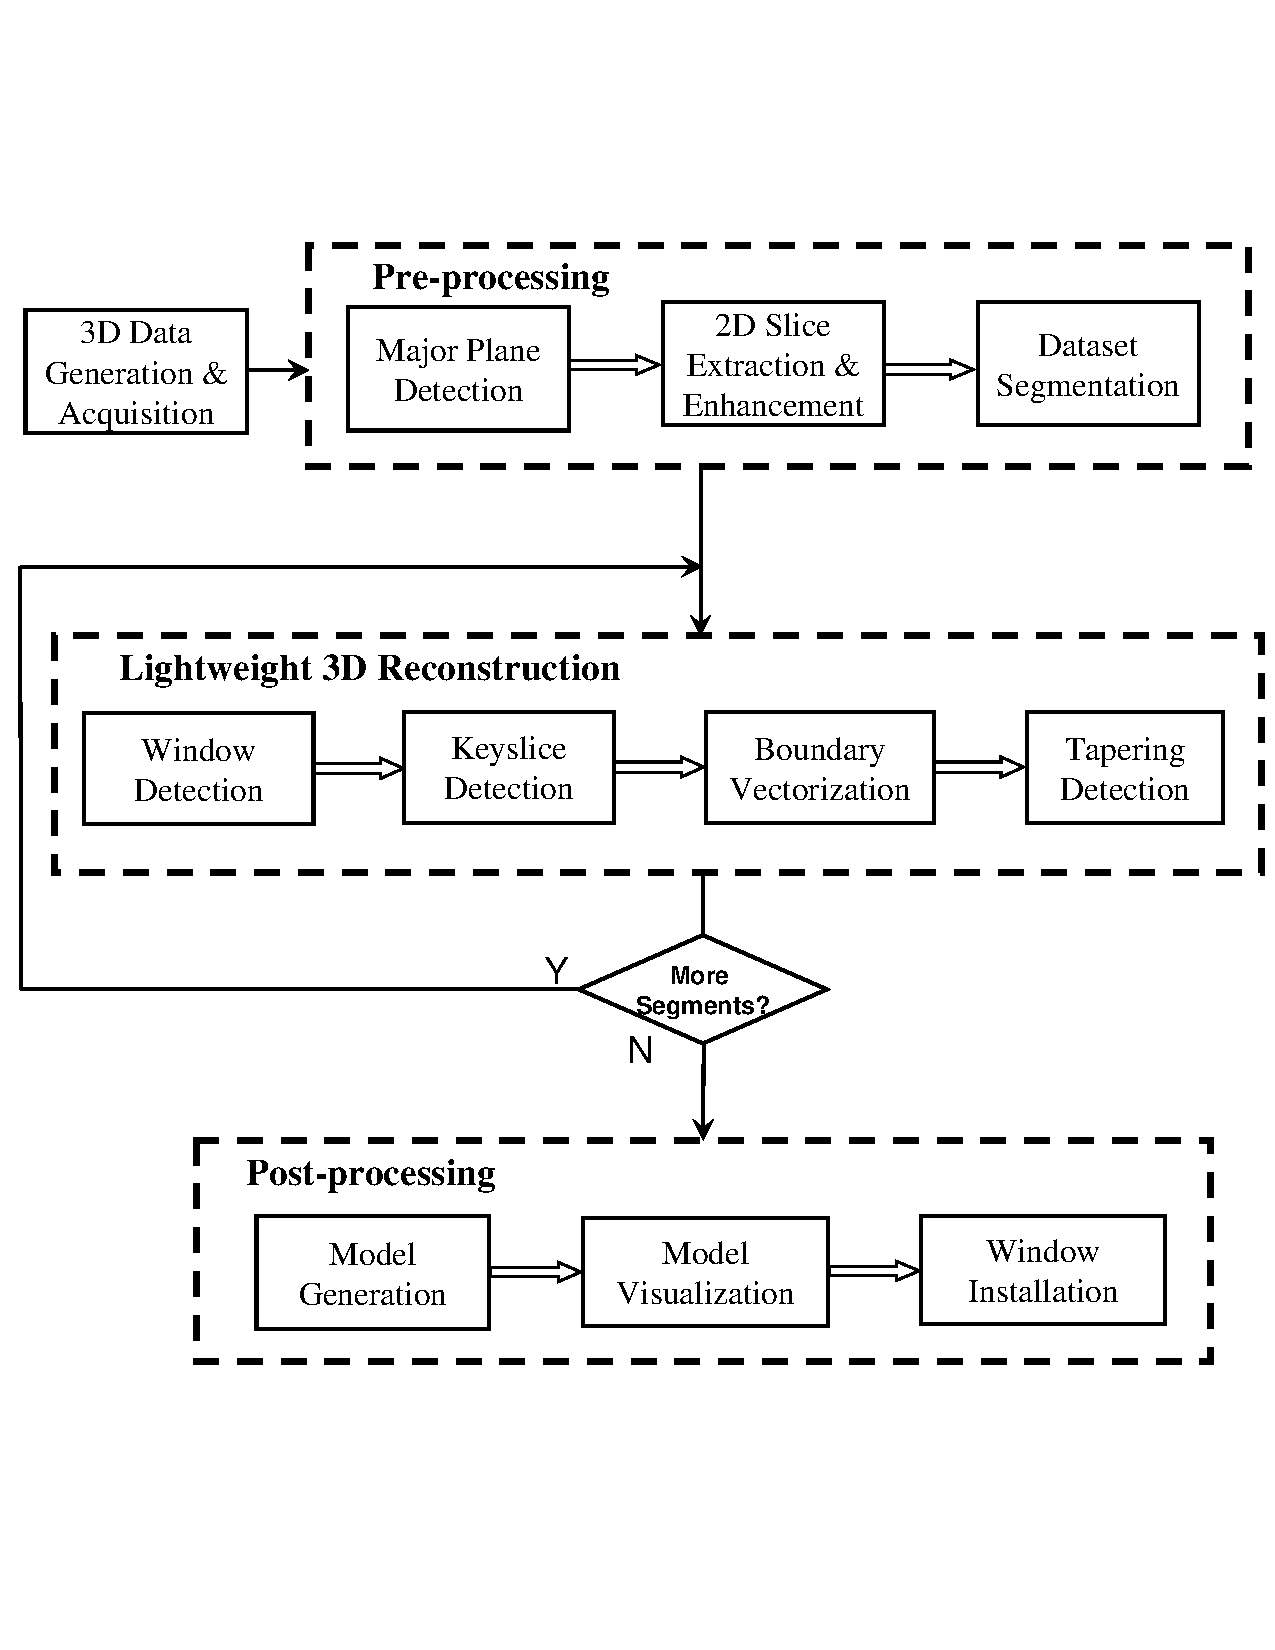
\includegraphics[width=\textwidth]{flow.pdf}
      \caption{Flow graph for proposed approach}
      \label{fig:flow}
\end{figure}

An overview of our approach, depicted in \Fig{ov}, begins with the
acquisition of a dense 3D point cloud $C$ of a building.
$C$ is then partitioned into a nonoverlapping set of volumetric slabs.
Each slab $S$ is associated with one projection plane $P$,
sitting at the base of $S$.
The purpose of partitioning $C$ is to establish a set of cross-sections,
or contour slices.
By examining the changes among these slices, we can identify the prominent
slices, or {\it keyslices}, as well as the necessary extrusion and
taper operations that must apply to them to generate the model.
By casting this 3D modeling task into a series of 2D operations, we
reduce the dimension of the problem to achieve a significant savings in
computational complexity.

To generate the 3D model of a building, all these key raster images need 
to be vectorized to represent the silhouette or boundary of the building. 
Couple of raster image vectorization approaches are
proposed in \cite{DP_AAKMT, DP_DP, DP_WM}. The Douglas-Peucker
algorithm tried to connect all the existed points to form a polygon. 
Although the implementation of
this approach is very efficient with the improvement in \cite{DP_HS},  this method cannot
handle the case where some extra interior points are existed as some outlier data.
To tackle this issue, Medeiros et al. \cite{BPA_MVL} applied ball-pivot algorithm (BPA)
\cite{BPA_BMRS}, which was original proposed on 3D point cloud data, on the 2D image to obtain
vectorized boundary. The key parameter for BPA to work successfully is to find the right size of
the ball for pivoting. We have proposed an adaptive BPA algorithm to solve this problem.

\begin{figure}[htbp]
\begin{center}
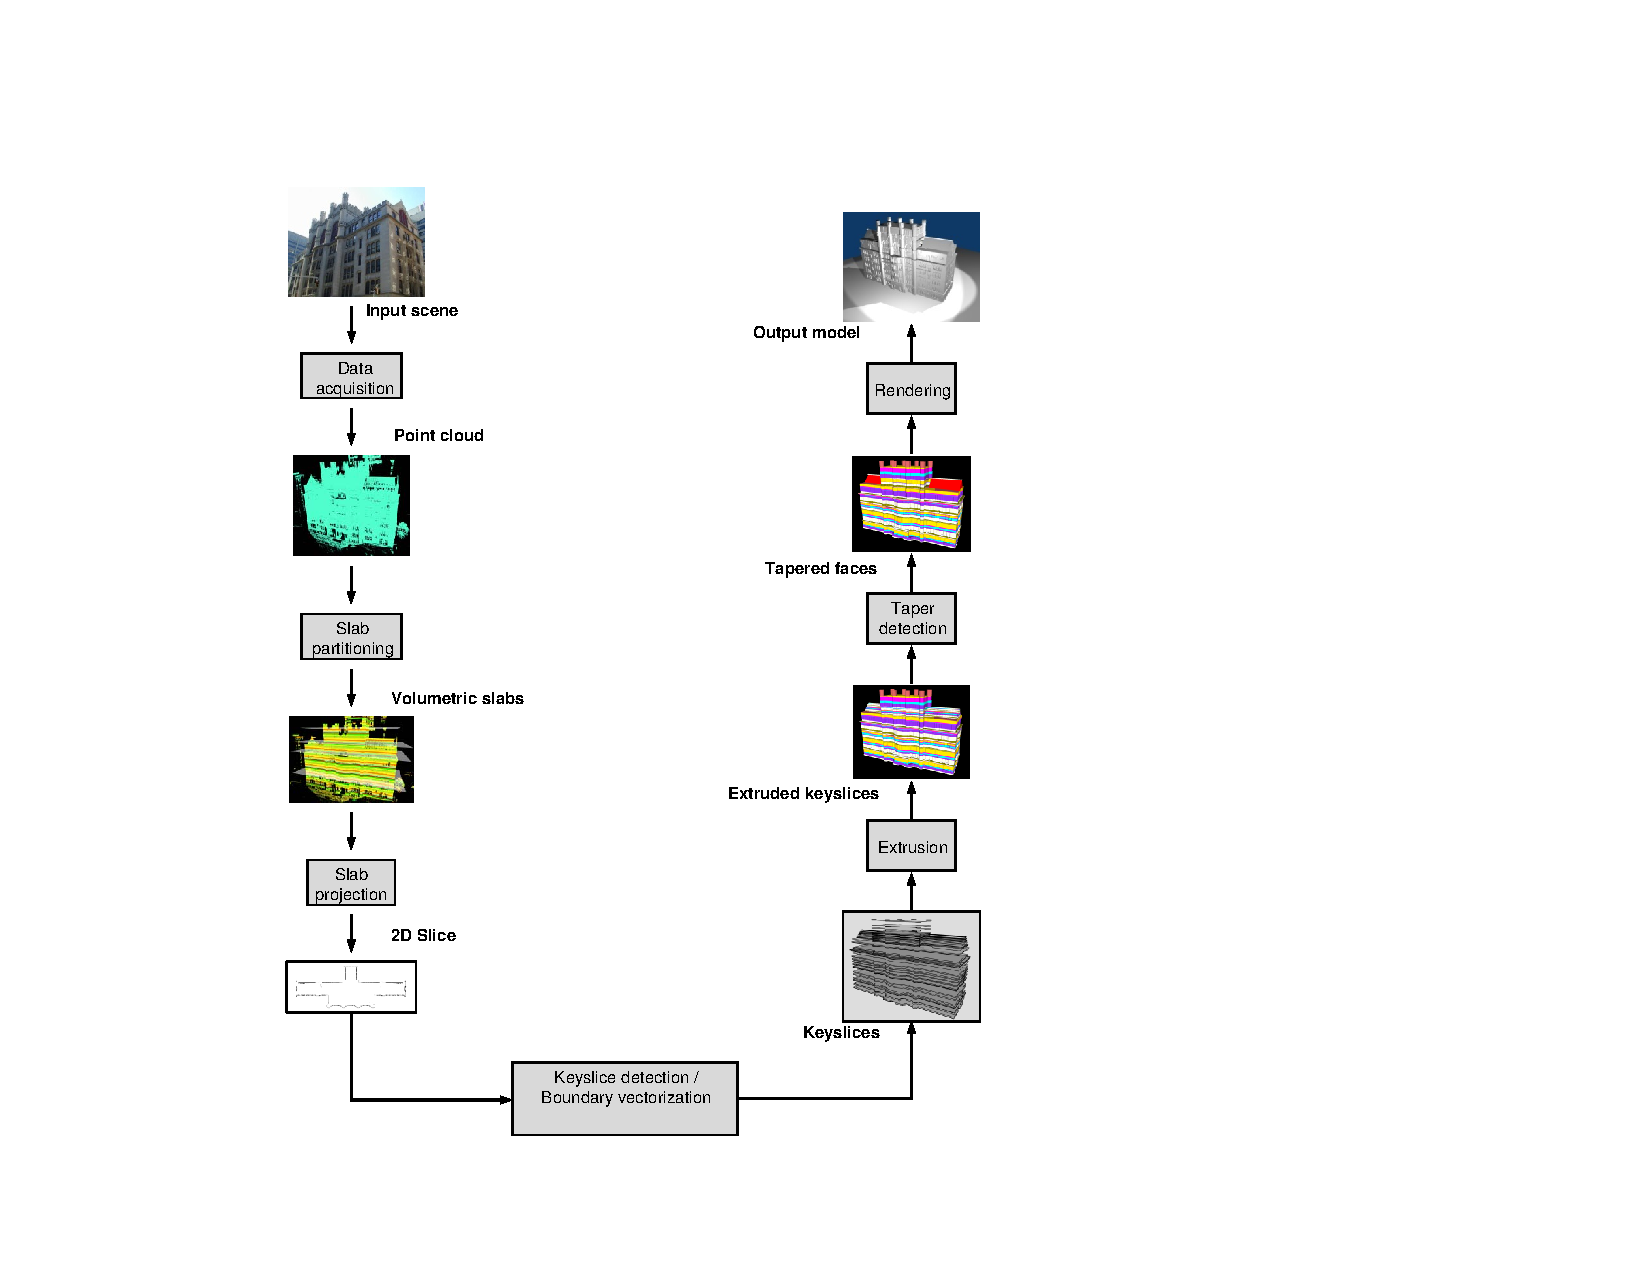
\includegraphics[width=1.0\textwidth]{overview.pdf}
\end{center}
\caption{Overview of the proposed approach.}
\label{fig:ov}
\end{figure}

Due to occlusion and material-dependent reflection problems off of glass
(e.g., windows), the input data is incomplete and noisy.
Therefore, noise removal and hole filling are carried out as a
preprocessing stage to generate the 3D model.
The next stage of the approach is to carry out fast image processing
techniques on the enhanced image slices to detect keyslices.
Boundary vectorization for these raster keyslices is then conducted to
transform these points into polygons.
Tapered structure detection is carried out to further reduce the model size.
Finally, 3D model generation is achieved by applying the extrusion/taper
operations to the keyslices to reconstruct lightweight 3D models of urban
buildings from range data.

\newchapt{Preprocessing on Range Data}{chapt2}{Preprocessing on Range Data}

%%%%%%%%%%%%%%%%%%%%%%%%%%%%%%%%
%%%%%%   PREPROCESSING  %%%%%%%%
%%%%%%%%%%%%%%%%%%%%%%%%%%%%%%%%
%\section{Preprocessing the Range Data}
\label{sec:prep}

The input to our system is range data assembled as a 3D point cloud.
Our data is obtained from a Leica Cyrax 2500 laser range scanner \cite{RDP_LRS},
which works by sweeping an eye-safe laser beam across the scene to collect
up to one million 3D depth points per frame.
All scene points that lie within 100 meters can be acquired with an accuracy
of 5mm in depth.
The basic algorithm that we use for registering the voluminous 3D data
acquired from multiple scans of buildings has been introduced in
\cite{RDP_LS}.
That same algorithm is also responsible for extracting the major axes
of the building in order to align it to the axes of the world coordinate
system.
This is necessary to properly infer the keyslices.
\Figb{IR_2_DXF} displays a properly aligned, {\it registered} 3D point cloud
consisting of 14 scans totalling 14 million points.

\begin{figure}[htbp]
\begin{center}
\begin{tabular}{c}
	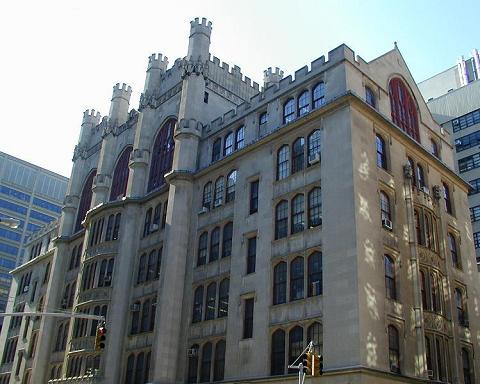
\includegraphics[width=0.6\textwidth]{HunterPhoto.jpg} \\
	(a)\\
	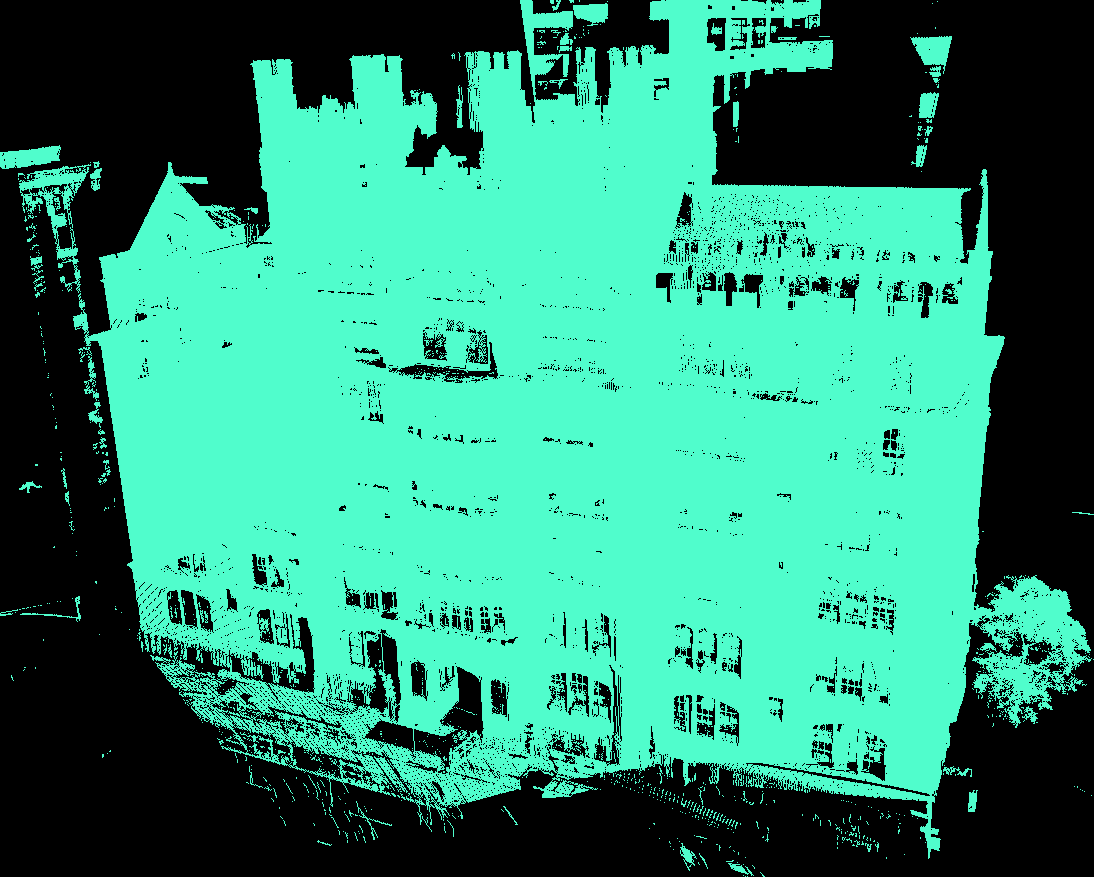
\includegraphics[width=0.6\textwidth]{point_cloud.png} \\
	(b)
\end{tabular}
\end{center}
\caption{
(a) Image of building to be modeled.
(b) 3D point cloud of building assembled by registering multiple scans.
}
\label{fig:IR_2_DXF}
\end{figure}

Due to occlusions and limited vantage points, the point cloud collected by the
laser scanner contains artifacts and holes.
In addition, computing directly on 3D data is time-consuming and
computationally complex.
To tackle these issues, we define inner and outer bounding boxes for the
building to clip away unrelated scene objects.
Then, we convert the 3D modeling problem into a set of 2D problems by
projecting the 3D data into a series of 2D cross-sectional contour images.
Noise removal, hole filling, and vectorization are all done in this
2D space.

%%%%%%%%%%%%%%%%%%%%%%%%%%%%%%%%
%%%%%% 3D Data Rectification %%%
%%%%%%%%%%%%%%%%%%%%%%%%%%%%%%%%
\section{Point Cloud Rectification}
\label{sec:rect}

%% Put the flow of the data rectification.
Although the multiple scans of point cloud data have been registered, 
they are not rectified as depicted in \Fig{pc_orig}. 
Please note the point cloud has been sub-sampling by a factor of 50.
This is not suitable for our further 3D modeling.
As one of the pre-processing steps, this registered data will be rotated
and translated to be aligned with world coordinates.

%% Put the image of rectfied data.
\begin{figure}[htbp]
\begin{center}
\begin{tabular}{c}
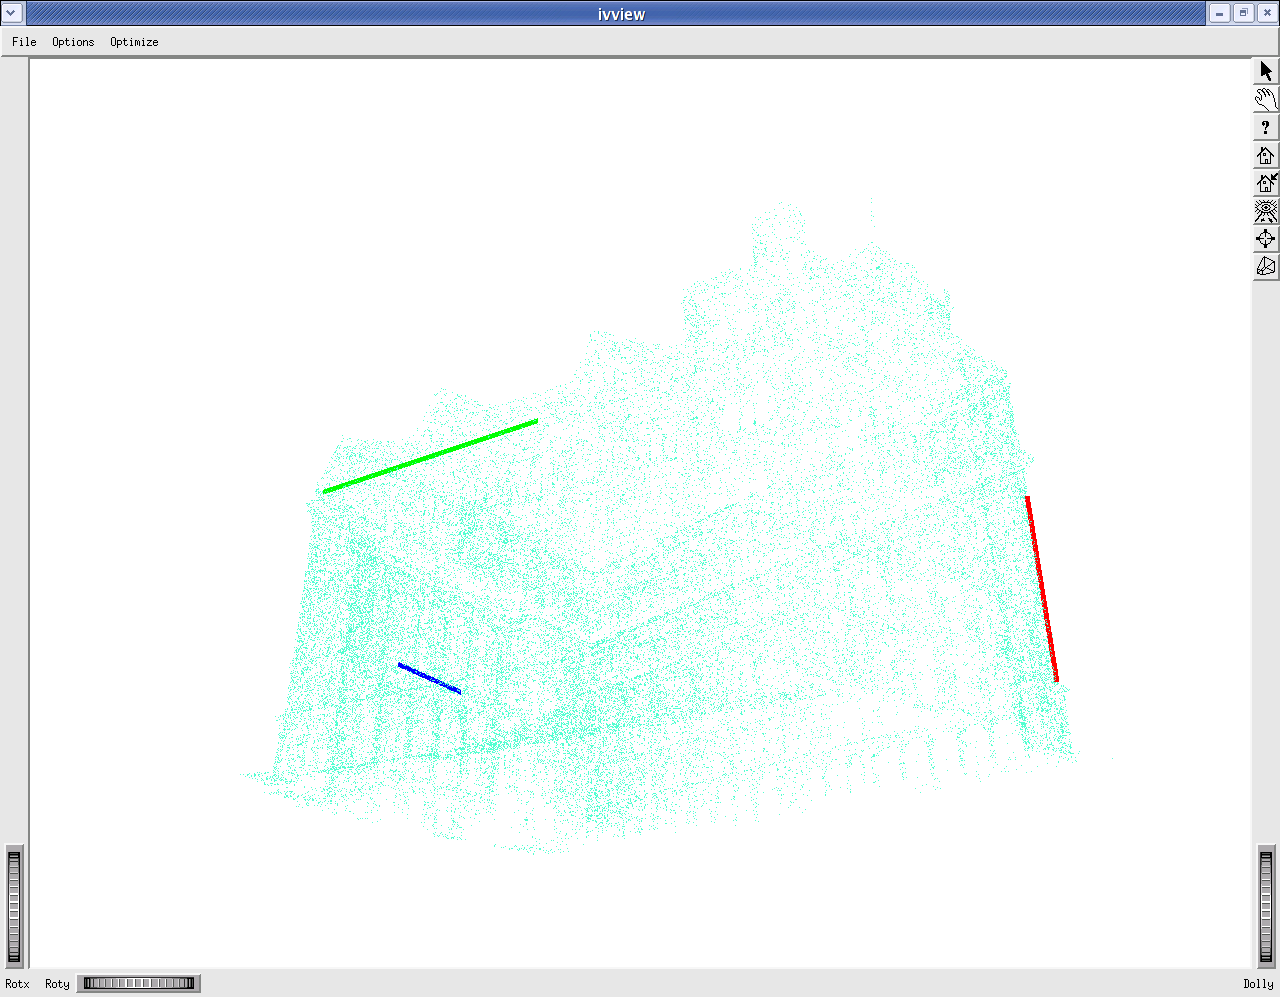
\includegraphics[width=\textwidth]{point_cloud_not_rect.png}
\end{tabular}
\end{center}
\caption{ The registered point cloud without rectification. }
\label{fig:pc_orig}
\end{figure}

As we know, there are a lot of line features existed in the point cloud, which
provides a good clue for rectifying the data. 
For each scan $s$ of the scene, we can obtain a set of line segments $L_s$. 
Assume $T_s$ is the transformation matrix for the scan $s$ to be registered with other scans.
In other words, for any point $P(x,y,z)$ in the scan $s$, $P*T_s$ will transform the
point $P$ into the final registered coordinate system as shown in \Fig{pc_orig}.

We can obtain the major axises by clustering these line segments $L_s$ from different
scans. The purpose of clustering is to group the lines whose direction are very close to each other.
To cluster these lines, we first transform the line segments in $L_s$ into world
coordinate system using $T_s$ as described above. After transformation, we will
get a larger line set $L = {l_1, l_2, \ldots, l_n}$. For each line $l_i$, we first
normalize it to a unit vector:
\begin{equation*}
\overline{l_i} = \frac{l_i}{\parallel l_i \parallel}
%% \bar --> \overline
\end{equation*}

The unit vector $\overline{l_i}$ has the unique length 1, which provides a good starting point 
for clustering since we do not need to worry about the length of the lines. 
An array of bins are used to hold the unit vectors.
As the initial step, the first line $\overline{l}$ is picked up and is insert into the 
first bin and set the counter of the bin to 1.
When a new unit vector $\overline{l_n}$ is observed, we try to see whether there is an
existed unit vector in the bins which has similar direction as $\overline{l_n}$. This is
done by computing the distance $d_{\pm}=\parallel \pm\overline{l_n} - \overline{l_i} \parallel$.
Because $\overline{l_n}$ can has two opposite directions, we can compute both of them and
choose the smaller value as the distance $d$. If $d$ is smaller enough, $\overline{l_n}$
is clustered with the line $\overline{l_i}$ and the counter of the bin holding $\overline{l_i}$
is increased by 1. On the other hand, if $d$ is big, we have to compare $\overline{l_n}$
with a line in the next bin. If $\overline{l_n}$ could not fit any line in the bins, we
will insert $\overline{l_n}$ into a new bin and set the counter of the bin to 1. 
To avoid the bias of the initial select, each unit vector $\overline{l_i}$ is
adjusted to be the mean of all unit vectors falling inside this bin. 

Once we go through all the lines in $L$, the clustering is complete. 
The next step is to choose the major axises from the clustering results. 
Essentially, this is to choose bins whose counters are among largest. 
Assume $u$, $v$, and $n$ represent the three largest bins. This is demonstrated in
\Fig{pc_orig} in red, green and blue respectively. To rectify the data,
we can refer to the following transformation matrix $\mathbf{M}$:
\begin{figure}[htbp]
\begin{center}
\begin{tabular}{c}
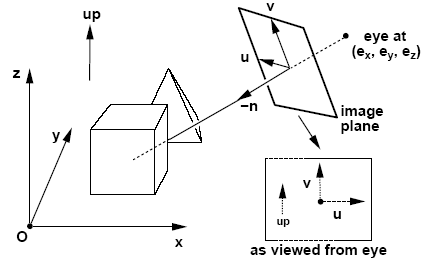
\includegraphics[width=0.5\textwidth]{point_cloud_rect_matrix.png}
\end{tabular}
\end{center}
\caption{ The transformation matrix. }
\label{fig:pc_rect_matrix}
\end{figure}

\begin{equation*}
\mathbf{M} = \left(
\begin{array}{cccc}
u_x & u_y & u_z & -e_x \\
v_x & v_y & v_z & -e_y \\
n_x & n_y & n_z & -e_z \\
  0 &   0 &   0 &    1 
\end{array} \right)
\end{equation*}

This is illustrated in \Fig{pc_rect_matrix}. $(x, y, z)$ is the world coordinate system.
The rectified coordinate system is represented using $(u, v, n)$. 
The vector $[-e_x, -e_y, -e_z]^T$ is the translation of the view point from the world origin.
After the transformation with $\mathbf{M}$, the new data set and the three major line segments are
shown in \Fig{pc_rect}.

%% rectified data
\begin{figure}[htbp]
\begin{center}
\begin{tabular}{c}
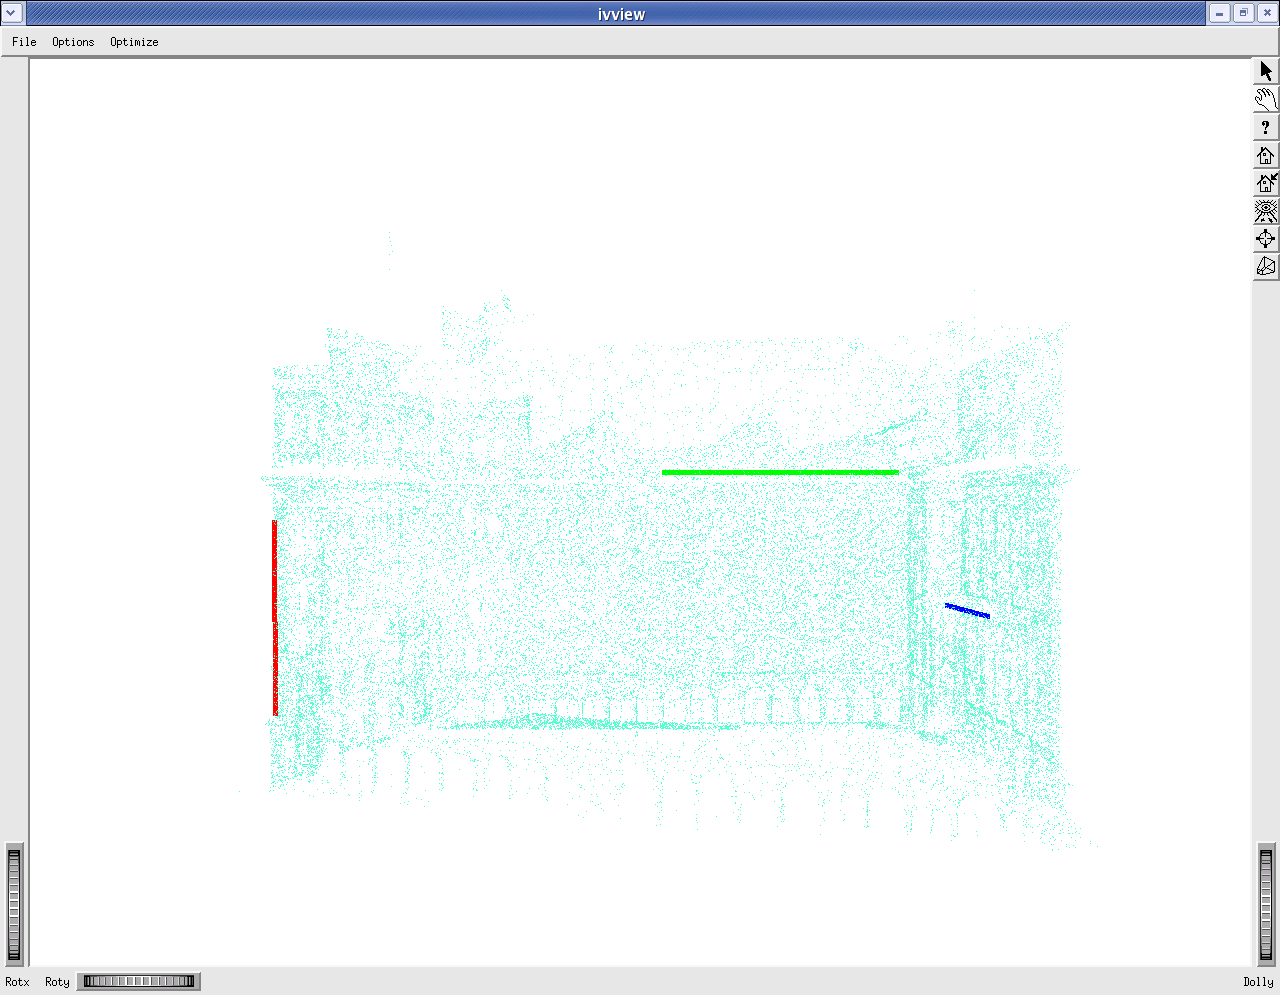
\includegraphics[width=\textwidth]{point_cloud_rectified.png}
\end{tabular}
\end{center}
\caption{ The rectified point cloud of \Fig{pc_orig}. }
\label{fig:pc_rect}
\end{figure}


\section{Extraction of 2D Slices}
\label{sec:image_slicing}

We consider the point cloud data as a large array of 3D points to be
sliced into horizontal volumetric slabs.
All 3D points within each slab are projected onto a horizontal projection
plane, or slice, at the base of the slab.
\Fig{slice_slab} shows the 3D point cloud in \Figb{IR_2_DXF} partitioned into
50 slabs.
The 3D points in each slab are projected onto a projection plane to
form cross-sectional contour slices.
\Fig{slicing} depicts four such slices, associated with the four displayed
projection planes of \Fig{slice_slab}.

\begin{figure} [htbp]
\begin{center}
\begin{tabular}{c}
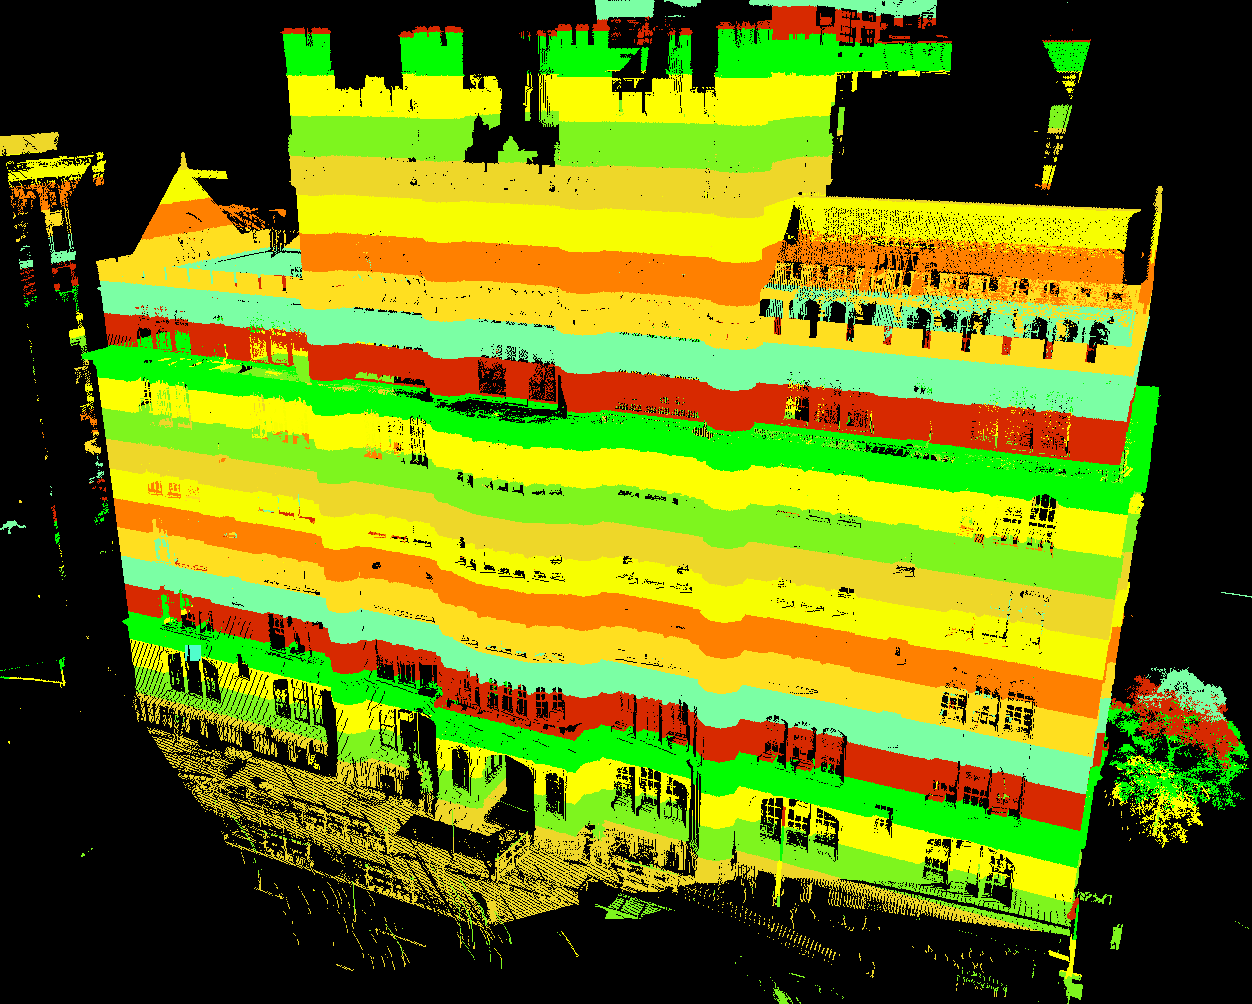
\includegraphics[width=0.6\textwidth]{slab_noplanar.png} \\
(a) \\
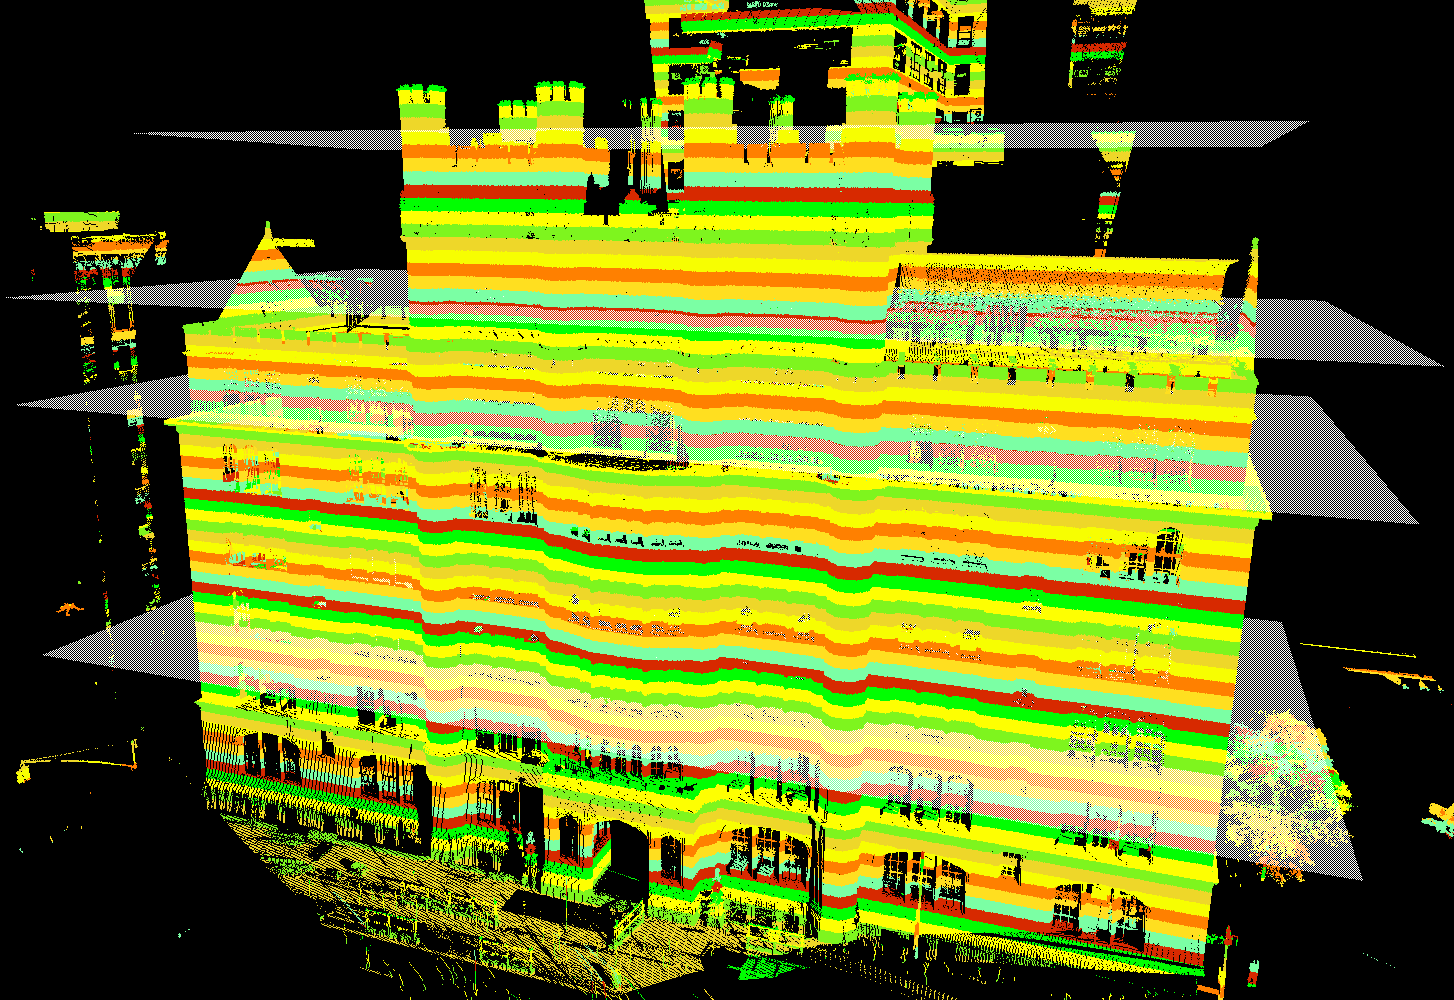
\includegraphics[width=0.6\textwidth]{slab_planar.png} \\
(b)
\end{tabular}
\end{center}
\caption{
(a) Slabs of the 3D point cloud data are used to determine prominent
cross-sections upon which extrusion/taper operations are applied.
(b)The 3D point cloud of \Figb{IR_2_DXF} partitioned into uniform
volumetric slabs.
The 3D points in each slab are projected onto a projection plane to
form cross-sectional slices. Four such planes are shown.}
\label{fig:slice_slab}
\end{figure}

The height of each slab is $\boldsymbol{\delta}$.
If $\boldsymbol{\delta}$ is held constant, each slice is generated from
equi-spaced slab intervals.
If $\boldsymbol{\delta}$ is allowed to vary, then we may
choose to allow for large values in parts of the structure that are similar,
and low values in regions that contain finer detail.
To avoid working on 3D data directly, a relatively small constant value
for $\boldsymbol{\delta}$ is chosen to generate 2D cross-sectional image slices.

\begin{figure} [htbp]
\begin{center}
\begin{tabular}{cc}
\fbox{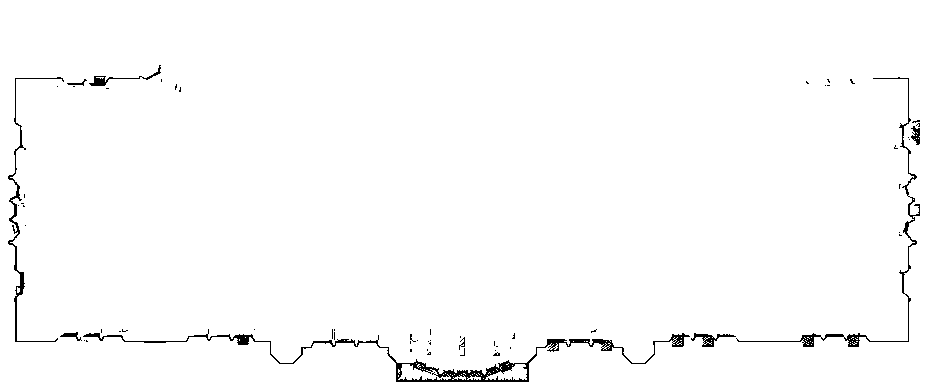
\includegraphics[width=0.45\textwidth]{image_slice_0190.png}} &
\fbox{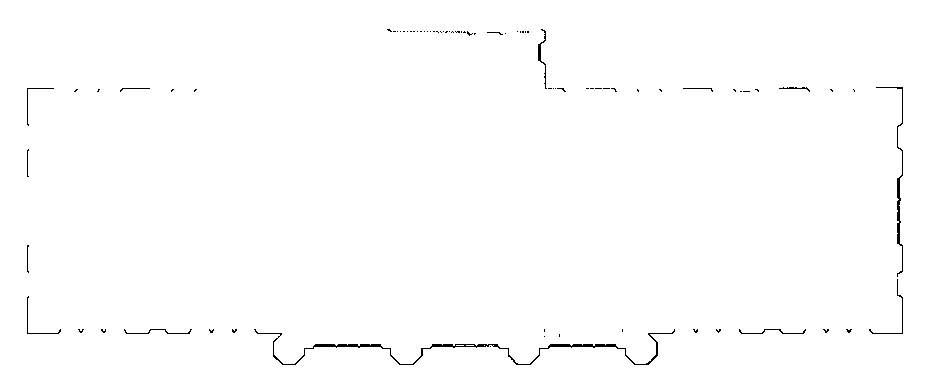
\includegraphics[width=0.45\textwidth]{image_slice_0600.png}} \\
(a) & (b) \\
\fbox{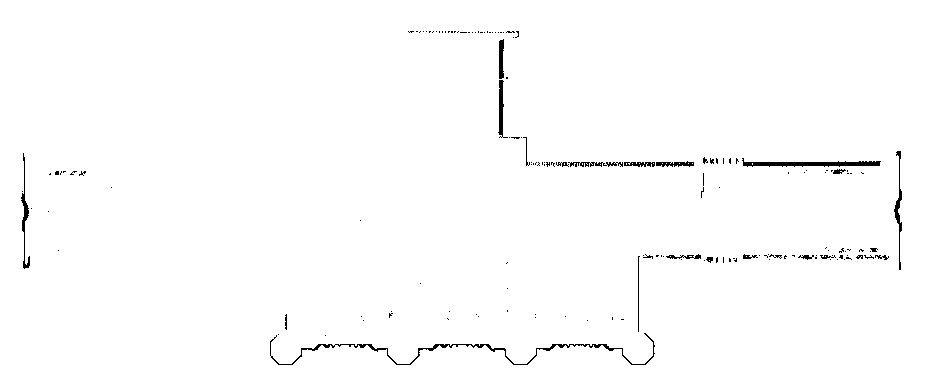
\includegraphics[width=0.45\textwidth]{image_slice_0714.png}} &
\fbox{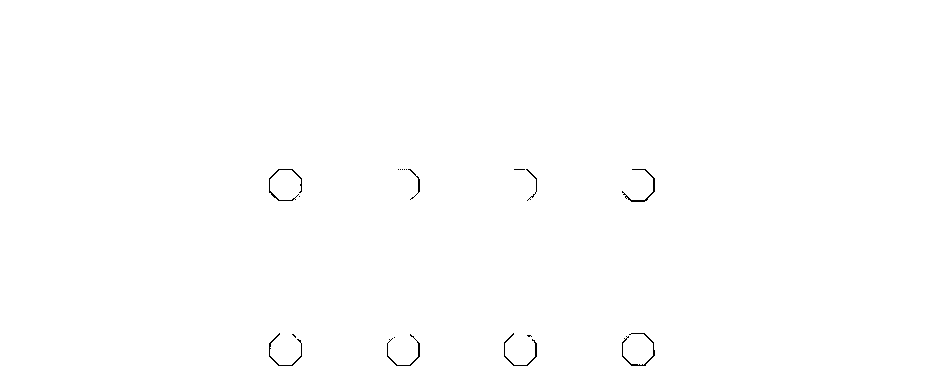
\includegraphics[width=0.45\textwidth]{image_slice_0951.png}} \\
(c) & (d)
\end{tabular}
\end{center}
\caption{The set of slices corresponding to the four projection planes in
\Fig{slice_slab}.}
\label{fig:slicing}
\end{figure}

Without loss of generality, the $y-$axis is used to represent the bottom-up
vertical direction.
Over each slab in height range $[H_{lo}, H_{hi})$,
we project the 3D data $\boldsymbol{P}(x,y,z)$, for $H_{lo} \leq y < H_{hi}$,
onto a 2D image slice.
The projection is normalized in the range $[0,W]$, where $W$ is the image width:
\begin{equation}
[\,x^{2D},\; y^{2D}\,]^T = \omega\cdot[\,x^{3D}_i - X_{MIN},\; z^{3D}_i - Z_{MIN}\,]^T
\label{eq:image_slicing}
\end{equation}
Note that $\omega = W/(X_{MAX} - X_{MIN})$, and that
the [$X_{MIN}$, $X_{MAX}$] and [$Z_{MIN}$, $Z_{MAX}$] pairs define the
3D bounding box, which can be obtained through user input and can be used
to clip away noise data.
\Fig{slicing}(a)-(d) show some examples of the 2D slices, where noise
and incomplete data are observed.

\newchapt{Slice Enhancement}{chapt3}{Slice Enhancement}

%%%%%%%%%%%%%%%%%%%%%%%%%%%%%%%%
%%%%%%   Slice Enhancement  %%%%
%%%%%%%%%%%%%%%%%%%%%%%%%%%%%%%%
\section{Hole Filling}
\label{sec:mdr}

The slices we extract above often have holes (i.e., missing data) due to
occlusion or other visibility issues.
Fortunately, most urban buildings have symmetry that we can exploit to
fill these holes.
Symmetry computation on 3D data is an active research topic, such as those in
\cite{Sym_PSGRF,Sym_ZPA,Sym_TW,Sym_MGP}, which has potentially numerous applications.
However, symmetry computation 3D data directly is expensive. 
Here, we only conduct this computation on the 2D image slices.
Since the 3D data has been already rectified \cite{RDP_LSYGS} 
and projected onto 2D slices, hence only 2D translation
is needed to be considered for symmetry computation.
Let $P(x,y)$ be a point on the original image $I$ and $P'(x',y')$ be the reflected
point of $P$ with respect to a symmetry line $L$.
The symmetry computation equation for $L$ is as follows:
\begin{equation}
L = \underset{x,y}{\operatorname{arg\,min}}\sum{d_{x,y}(P', I)}
\end{equation}
where the $d_{x,y}(P',I)$ is the distance between the self-reflected point
$P'$ and its nearest data point in image $I$.
The reflected point $P'$ of the original point $P$ is computed with
respect to a line along either the $x-$ or $y-$ axis.
Therefore, the symmetry line $L$ is obtained as the line with minimum
summation error over the reflected data points.
\Figa{sym} and \Figb{sym} depict the original input with holes, and
the output after hole filling using symmetry computation, respectively.

\begin{figure}[htbp]
\begin{center}
\begin{tabular}{c}
\fbox{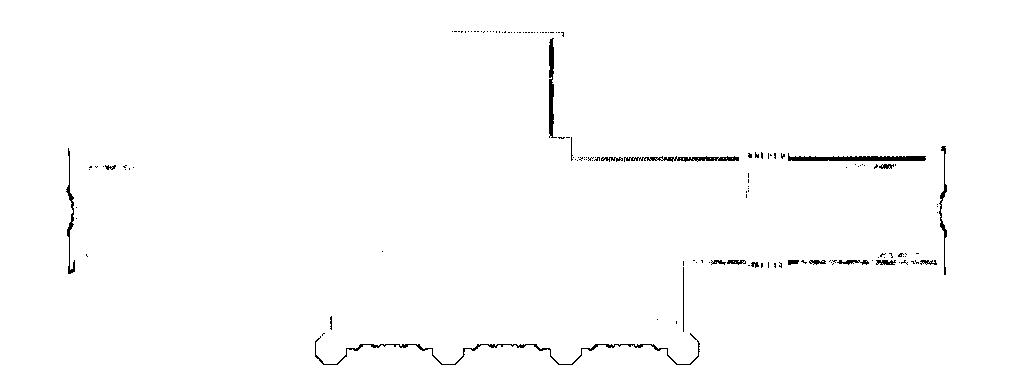
\includegraphics[width=0.6\textwidth]{image_slice_0705_0711.png}} \\
(a) \\
\fbox{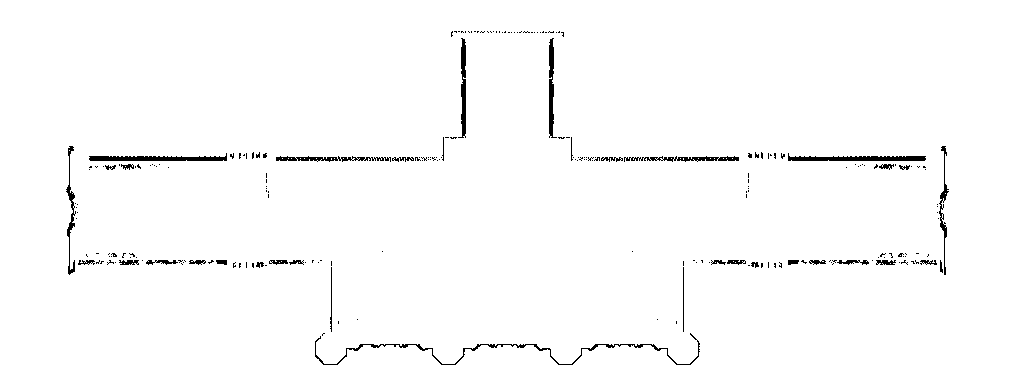
\includegraphics[width=0.6\textwidth]{image_slice_0705_0711_recoverd.png}} \\
(b)
\end{tabular}
\end{center}
\caption{ Symmetry-based hole filling. (a) Original 2D slice image and
(b) output image after hole filling.}
\label{fig:sym}
\end{figure}

\newchapt{Keyslice Detection}{chapt4}{Keyslice Detection}

%%%%%%%%%%%%%%%%%%%%%%%%%%%%%%%%
%%%%%%   3D Reconstruction  %%%%
%%%%%%%%%%%%%%%%%%%%%%%%%%%%%%%%
%\section{Lightweight 3D Reconstruction}
\label{sec:reconst}
Our 3D modeling algorithm is based on \emph{a priori} knowledge that
urban buildings can be created through a series of extrusion and taper
operations on the salient cross-sections contained in the keyslices.
\Fig{keyslices} depicts the keyslices derived from the uniform slices
given in \Fig{slice_slab}. 
The key step for successful modeling is identifying these salient cross
sections upon which the extrusion and taper operations will apply.

An intuitive way for key slice detection is to 
compute the similarity between the sliced images.
In other words, the sliced images are clustered into different groups 
based on the similarity among them.
There are two mainly research methods for similarity measurement of 2D images: 
area based method and feature based methods. 
The area based methods are computational efficient 
but they usually can only be applied on binary or gray-scale images. 
The feature based one is computational complex but more powerful 
and can be applied to images obtained using different sensors, 
such as multi-modal image registration.
% read similarity measure papers.
Because our goal is to develop light-weight efficient algorithm for model reconstruction, 
plus the input for similarity measure is pure binary images, 
the area based method is adopted for our approach.

The classical measurement for area based method is the normalized cross
correlation \cite{DIP_Pratt}:
\begin{equation*}
CC(i,j) = \frac{\sum_W(W - E(W))(I_{(i,j)}-E(I_{(i,j)}))}
{\sqrt{\sum_W(W - E(W))^2}\sqrt{\sum_{I_{(i,j)}}(I_{(i,j)} - E(I_{(i,j)}))^2}}
\end{equation*}
where $W$ is an image mask, $E(W)$ is the mean of the mask's pixels, 
and $E(I_{(i,j)})$ is the mean of the image pixels covered by the mask $W$.
However, this method is very time consuming and is a local window-based approach,
which could not capture the global relations between images. 
Therefore, we proposed a light-weighted global and efficient key image detection approach 
based on Hausdorff distance and curvatures computation.

\begin{figure}[hbtp]
\centering
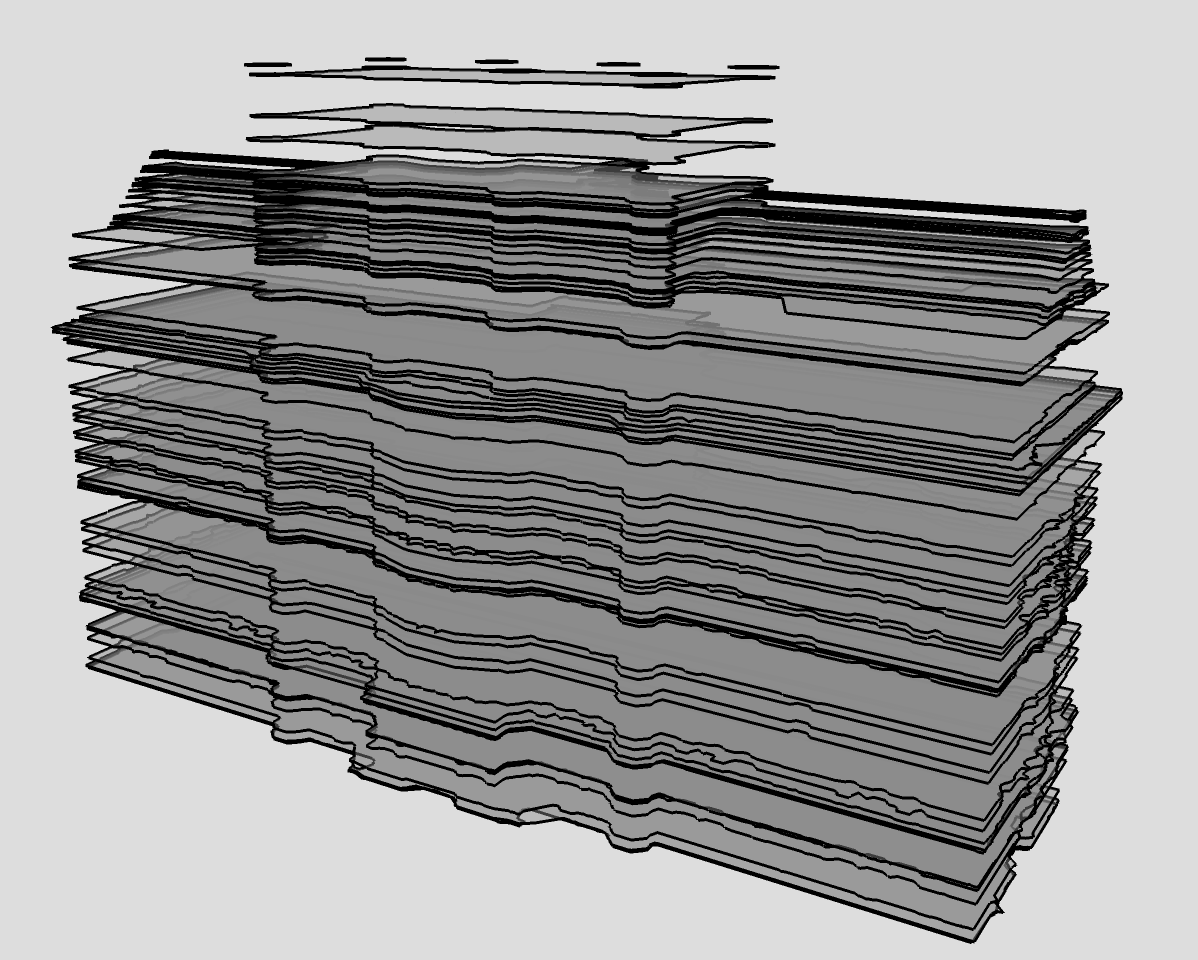
\includegraphics[width=0.8\textwidth]{figures/keyslice_wireframe.png}
\caption{Keyslices derived from the input in \Fig{slice_slab}.}
\label{fig:keyslices}
\end{figure}

\section{Hausdorff Distance Based}
\label{sec:ksd}
The 2D image slices of an extruded region are similar to each other.
Thus, to detect the keyslices that delimit extruded regions one only needs
to compute the similarity between adjacent slices.
We select the Hausdorff distance \cite{IR_HKR} as the similarity measurement.
Let $P_r(x_r, y_r)$ be a data point in a reference image and
let $P_i(x_i, y_i)$ be a data point in a new observed image $I$.
The Hausdorff distance of image $I$ to reference image $I_r$ is defined as:

\begin{equation}
d_H(I, I_r) = \sum_{i=0}^Nd_{min}(P_i, I_r)
\label{eq:hd}
\end{equation}

where $d_{min}(P_i, I_r)$ is the minimum distance from data point $P_i$
in image $I$ to the reference image $I_r$.
Alternatively, we can also define the Hausdorff distance, $d_H(I_r, I)$,
from reference image $I_r$ to a new observed image $I$, using \Eq{hd}.
These two distances are usually not equal to each other.
As a rule of thumb, one can choose
$d_{HD} = \text{MAX}\{d_H(I, I_r), d_H(I_r, I)\}$ as the Hausdorff distance.
To compute the keyslices, a threshold $\tau_{d}$ is used for the
Hausdorff distance $d_{HD}$.
If $d_{HD} < \tau_{d}$, the two images $I$ and $I_r$ are considered
similar to each other.
Otherwise, a keyslice image is found and $I_r$ is updated with $I$,
the new keyslice image.

\section{Curvature Based}
The accuracy of the keyslices detected by using the Hausdorff distance
is closely tied to threshold $\tau_d$.
Small $\tau_d$ leads to more accurate models and will require more time and
space to compute and store the result.
When the threshold $\tau_d$ is relatively large, potential keyslices which
contain salient structure may be missed.
Therefore, there is a trade-off between model accuracy and time-space
efficiency.
To address this problem, the curvature information is computed as a
complementary criteria for keyslice detection.

This idea is based on the observation that the keyslices are generally
located at large curvature changes along 2D slices extracted in the orthogonal
direction (e.g., side view), as shown in \Figa{HT_BPA_Curvature}.
Therefore, instead of computing the difference between two images directly,
we compute the curvature of orthogonal 2D slices, map the positions of
curvature extrema back to cross-sections in the original set of volumetric
slabs, and mark these cross-sections as keyslices.

\begin{figure}[htbp]
\begin{center}
\begin{tabular}{cc}
\fbox{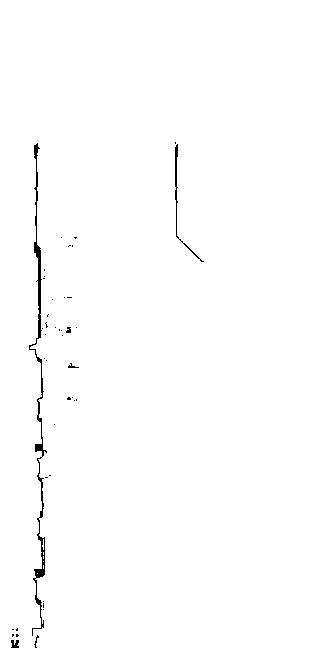
\includegraphics[width=0.3\textwidth]{image_slice_lr_0580_0590_half.jpg}}
\fbox{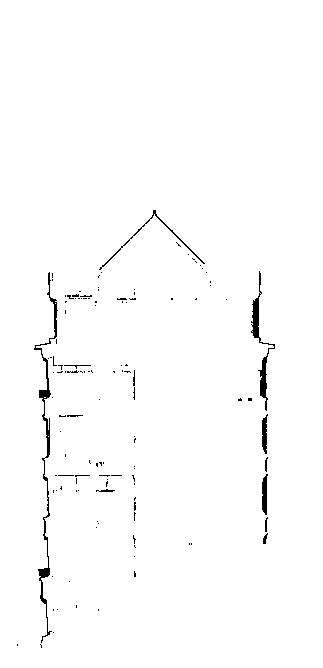
\includegraphics[width=0.3\textwidth]{image_slice_lr_0830_0842_half.jpg}} &
\fbox{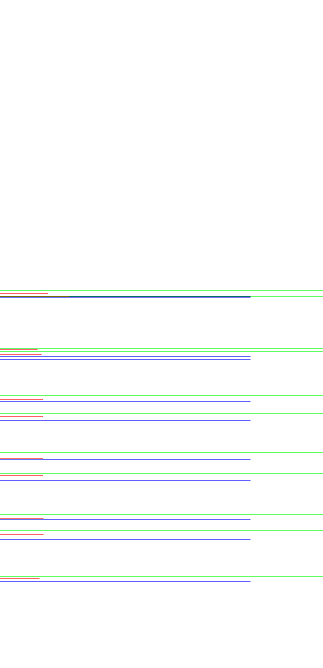
\includegraphics[width=0.3\textwidth]{curvature_center_lines_old_half.jpg}} \\
(a) & (b)
\end{tabular}
\end{center}
\caption{Curvature-based key slice detection.
(a) A partial set of two 2D sliced images from the orthogonal direction (side
view). The complete set will be used to extract the keyslices shown in
\Fig{keyslices}.
(b) The average curvatures detected over all of the sliced images along the
orthogonal direction.}
\label{fig:HT_BPA_Curvature}
\end{figure}

In the close-up view of a small region as shown in \Fig{KSD_Curv},
two curvatures, $c_1$ and $c_2$, are
computed in this small region. The red, blue and green lines indicate the locations
of the center, the starting and the ending of a curvature. 
As a matter of fact, there is a third curvature computed around the
black box sitting on top of the green line of the curvature $c_1$. 
However, this third one should not be consider as a real curvature 
in that the black box is due to an air conditioner during the data acquisition process, 
which means it is not a part of the building. We called this third curvature
{\it outlier curvature} which needs to be removed from the set of real curvatures.
Based on the fact that these outlier curvatures exist only in a few 2D slices,
we can exclude them by counting the number of appearance for each curvature.
Only those curvatures appears in most of the 2D slices are kept for further computation.

Once the real curvatures are obtained, they can be used as a complemental way of 
Hausdorff distance for keyslices detection. 
Each curvature $c$ is mapped to a set $s$ of original 2D cross-sectional
slices, $i,\ldots,j$, where $i$ and $j$ are corresponding to the starting and 
the ending locations of $c$. After this, the set $s$ is checked whether 
it contains any keyslice or not.
If a keyslice $k$ has been marked in $s$ by Hausdorff distance, 
nothing needs to be done and this curvature $c$ is discarded. 
On the other hand, if $s$ contains no keyslice, $i$ and $j$ will be marked as 
two new keyslices to keep the salient feature identified by this curvature $c$.
The combination of Hausdorff distance measurement and curvature inference
ensures that the salient structures of a building will be preserved.

%%% Figure of the tapered template.
\begin{figure}[htbp]
\begin{center}
\begin{tabular}{c}
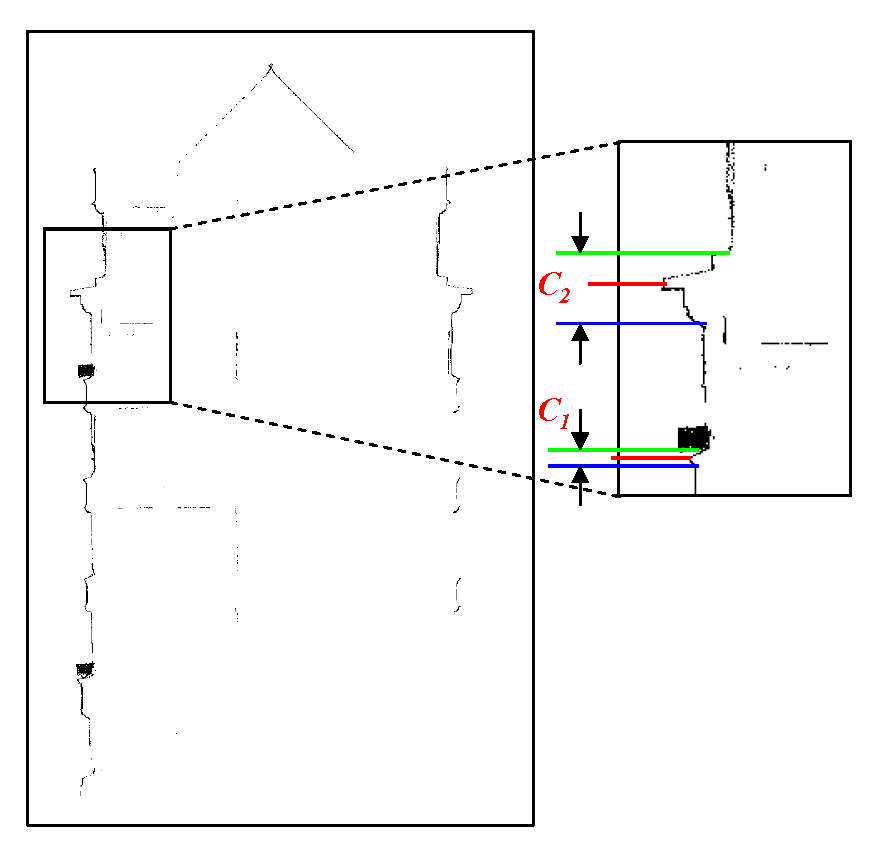
\includegraphics[width=0.60\textwidth]{curvature.png}
\end{tabular}
\end{center}
\caption{ Curvature based key slice detection. }
\label{fig:KSD_Curv}
\end{figure}
%%% End of Figure

To compute the curvature, we first apply the slice extraction algorithm
described in \Sec{image_slicing} to obtain a series of 2D cross-sectional
images in the orthogonal direction.
We then apply the ball-pivot algorithm described in \Sec{BPA} to
vectorize the boundary for each sliced image.
We locate those curvatures that appear in most of the sliced images as the
places where keyslices are found, as shown in \Figb{HT_BPA_Curvature}.
Note that the red lines indicate location of the center of the curvature,
and the blue and green lines indicate the entering and exiting of the
curvature structures, respectively.
The combination of Hausdorff distance measurement and curvature inference
ensures that the salient structures of a building will be preserved.

\section{Local Matching Based on Segmentation}

The keyslice detection described above are based on global information matching.
The strength of these methods lies on the effective of computation and they can
also produce good results on exterior scanning as depicted in %\Fig{keyslices}. 
However, when applied to interior scannings when the layout of the structures 
is complex, there may be some limitations on these methods. 
As depicted in %\Fig{ksd_gbl_bad}, the pillars inside the hall can be reconstructed
by simple extrusion of the base polygon. However, they are divided to 
excessive amount of keyslices because the dissimilarity of the outside window
structures in the same projection level. In other words, due to global matching
strategy, some independent objects which could be modeled using simple extrusion
operation are modeling using excessive keyslices. Although the reconstructed
models are still correct at this situation, they are not efficiency. That is, much
more keyslices are created to represent the simpled extruded parts. 

A more effective way for modeling the above structures is to model the different 
structures individually. By doing this, we can simply model the pillars using a
extrusion operation based on a base polygon. Certainly, for the complicate window
structures, more keyslices are still required but these keyslices would not contain
any pillar structures. To do this, segmentation is a necessary step to identify
all different parts of the scannings. 

There are a lot of literatures on image segmentation as in %\cite{segmentation}. 
% a little bit survey on image segmentation, especially binary image segmentation.
% why the graph-cut is well-fit for our purpose.

Our segmentation based keyslice detection approach is an iterative algorithm.
We first applied the graph cut
on the 2D sliced binary image. The initial input to graph cut is done as follows. 
First of all, a random data point $p$ was located in the binary image $I$. The data
point $p$ is then growing to form an region $r$ based on the connected components 
until it reaches a fix-point. That is, no more data point can be reached in $r$. $r$
is taken as input by graph cut algorithm to compute the segmentations. 
The segmented objects (non-background pixels) are then stored and their pixels are 
reset to background pixels for next iteration. The algorithm is depicted in %\Fig{alg_seg}.
To adjust the accuracy of the graph cut, the parameter ??? was used. To get more
accurate segments, which means more objects may be classified, enlarge/shrink its value.

For each new 2D image slice, there is a set of segmented objects $s$ is computed
by the above graph cut approach. Therefore, the keyslice detection problem is converted
into similarity measurement of the detected segments along the specified direction, 
e.g., vertical direction.
The similarity measurement is now among the segmented regions instead of the whole
contour of a sliced image. A global data structure, $T$, which contains all the current 
active segmented objects is maintained for matching. $T$ is initialized with the
detected segments from the first 2D slice which is regarded as reference slice. 

For each new observed 2D slice, we first compute a set of segmented objects $s$. 
After this, we are trying to search for a matched segmented object $o'$ in $s$ for 
each existed active segmented objects $o$ in $T$. This searching process again is 
based on the Hausdorff distance as described in \Sec{ksd}. If such a matched object $o'$
exists, $o$ will be kept in $T$ as an active segmented object for next round of
computation. Otherwise, $o$ is removed from $T$ and is treated as a completed part or
object in the range data. At the same time, for any object $o'$ in $s$, if it is 
not found to be a matched segments for active objects in $T$, $o'$ will be added
to $T$ as a starting slice of a new part in range data and will be taken into
account for next adjacent 2D slice computation. We keep doing this until the last
2D slice is visited and processed. Once the last slice is reached, all the active
segments in $T$ will be considered as the ending point of the objects in the range data.

The result obtained by the above local based keyslice detection is illustrated in 
%\Fig{ksd_lcl_good}. As we can see, the pillar structures of the hall are reconstructed
using the simple extrusion operations, which is much more efficient in terms of 
model size and representation.







\newchapt{Boundary Vectorization}{chapt5}{Boundary Vectorization}

After the keyslices are detected, $N_K$ keyslices will be identified
from a total of $N_A$ image slices.
Depending on the threshold $\tau_{d}$, $N_K$ is usually about one to two
orders of magnitude smaller than $N_A$, e.g., $N_K/N_A$ is 0.06 when
$\tau_d$ = 4.0 for the example in \Figb{IR_2_DXF}.
To generate the 3D model, these keyslice images need to be vectorized to
represent the contours of the building facade.
The difficulty of the problem lies in outliers and holes of non-perfect images.
We proposed a general framework based on an adaptive 2D ball-pivot algorithm (BPA) 
 to efficiently suppress the noisy, fill holes and generate contours for those images.

\section{Ball Pivot Algorithm (BPA)}
\label{sec:BPA}

STARTING POINT SELECTION
\\
\\
GAP DETECTION
\\
\\
RIGHT ANGLE RESHAPE
\\
\\


There exists numerous works on boundary vectorization,
such as those described in \cite{DP_RP,DP_LC,DP_AAKMT}.
However, these approaches
only consider the cases where perfect raster image data is provided.
For non-perfect data, these proposed methods were failed in various cases.
The problem considered here is to compute contours
for non-perfect binary images which may contain holes
along the boundary as well as noise or outliers
inside the boundary. Here, {\it boundary} refers to the
out-most region of any raster image and
{\it contour} refers to a vectorized boundary.


The Douglas-Peucker (DP) algorithm \cite{DP_DP} is widely used
to compute boundary vectorization for binary images.
Although  with the improvement of implementation described in \cite{DP_HS, DP_HS94},
the complexity of this approach is of $O(nlogn)$, this method cannot fill the
holes of the noisy data or handle the case
where spurious interior points are presented.
Agarwal et al. \cite{DP_AV} considered the problem of
approximating a polygon chain using another one to minimize the number of
vertices. However, for a raster image, the vertices
defining the contour were not known.
For example, \Figa{failed_case} shows a binary cross-section
image of a 3D point cloud data of a building. \Figb{failed_case} shows
the contour generated from DP algorithm. The problem is that there are
a lot of holes along the contour and the noise data inside of the
boundary are modeled inappropriately.
To tackle these issues, a general boundary vectorization framework is proposed
based on ball-pivoting algorithm (BPA) \cite{BPA_BMRS} which was used
originally on 3D point cloud data process to generate 3D mesh representation.
\Figc{failed_case} shows
the contour computed by the proposed framework which fills holes between gaps
and suppresses noise inside the boundary.


\begin{figure*}[hbtp]
\begin{center}
\begin{tabular}{c}
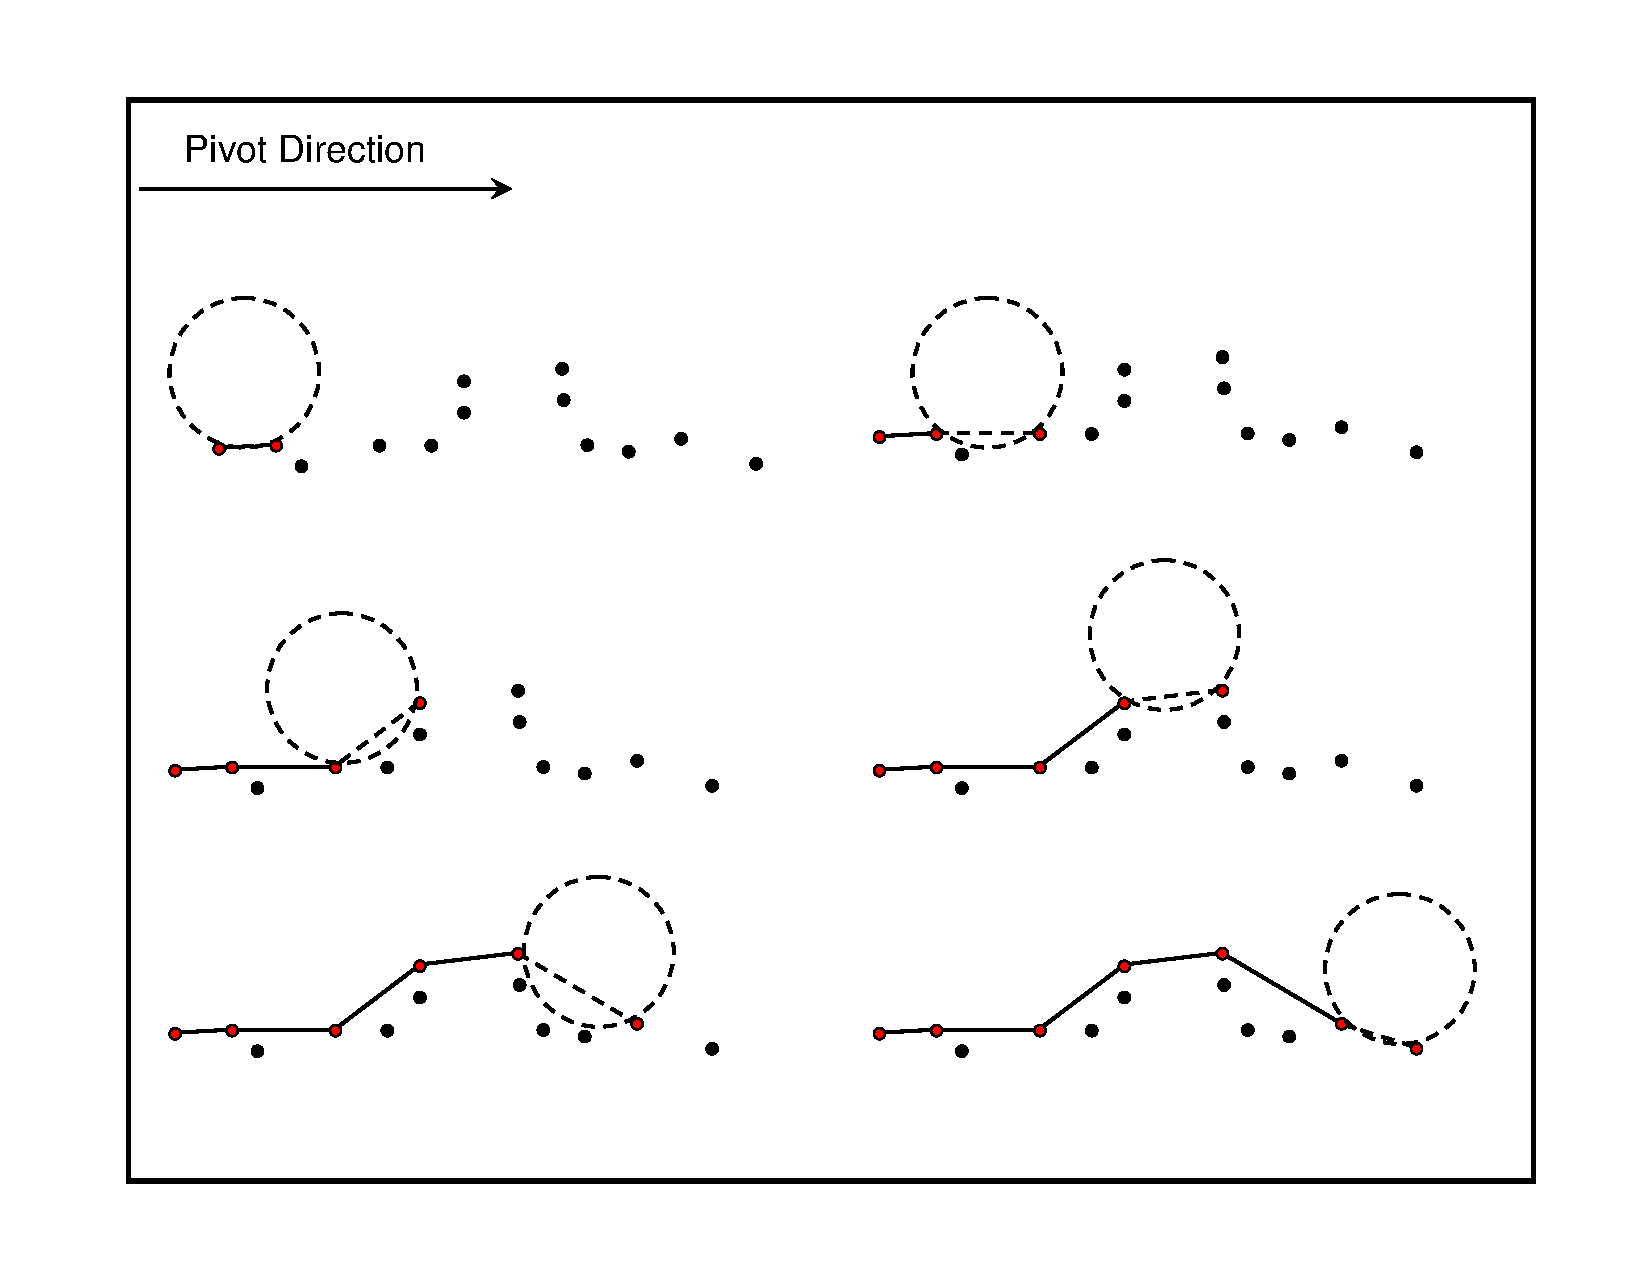
\includegraphics[width=0.8\textwidth]{BPA_init.pdf} \\
(a) \\
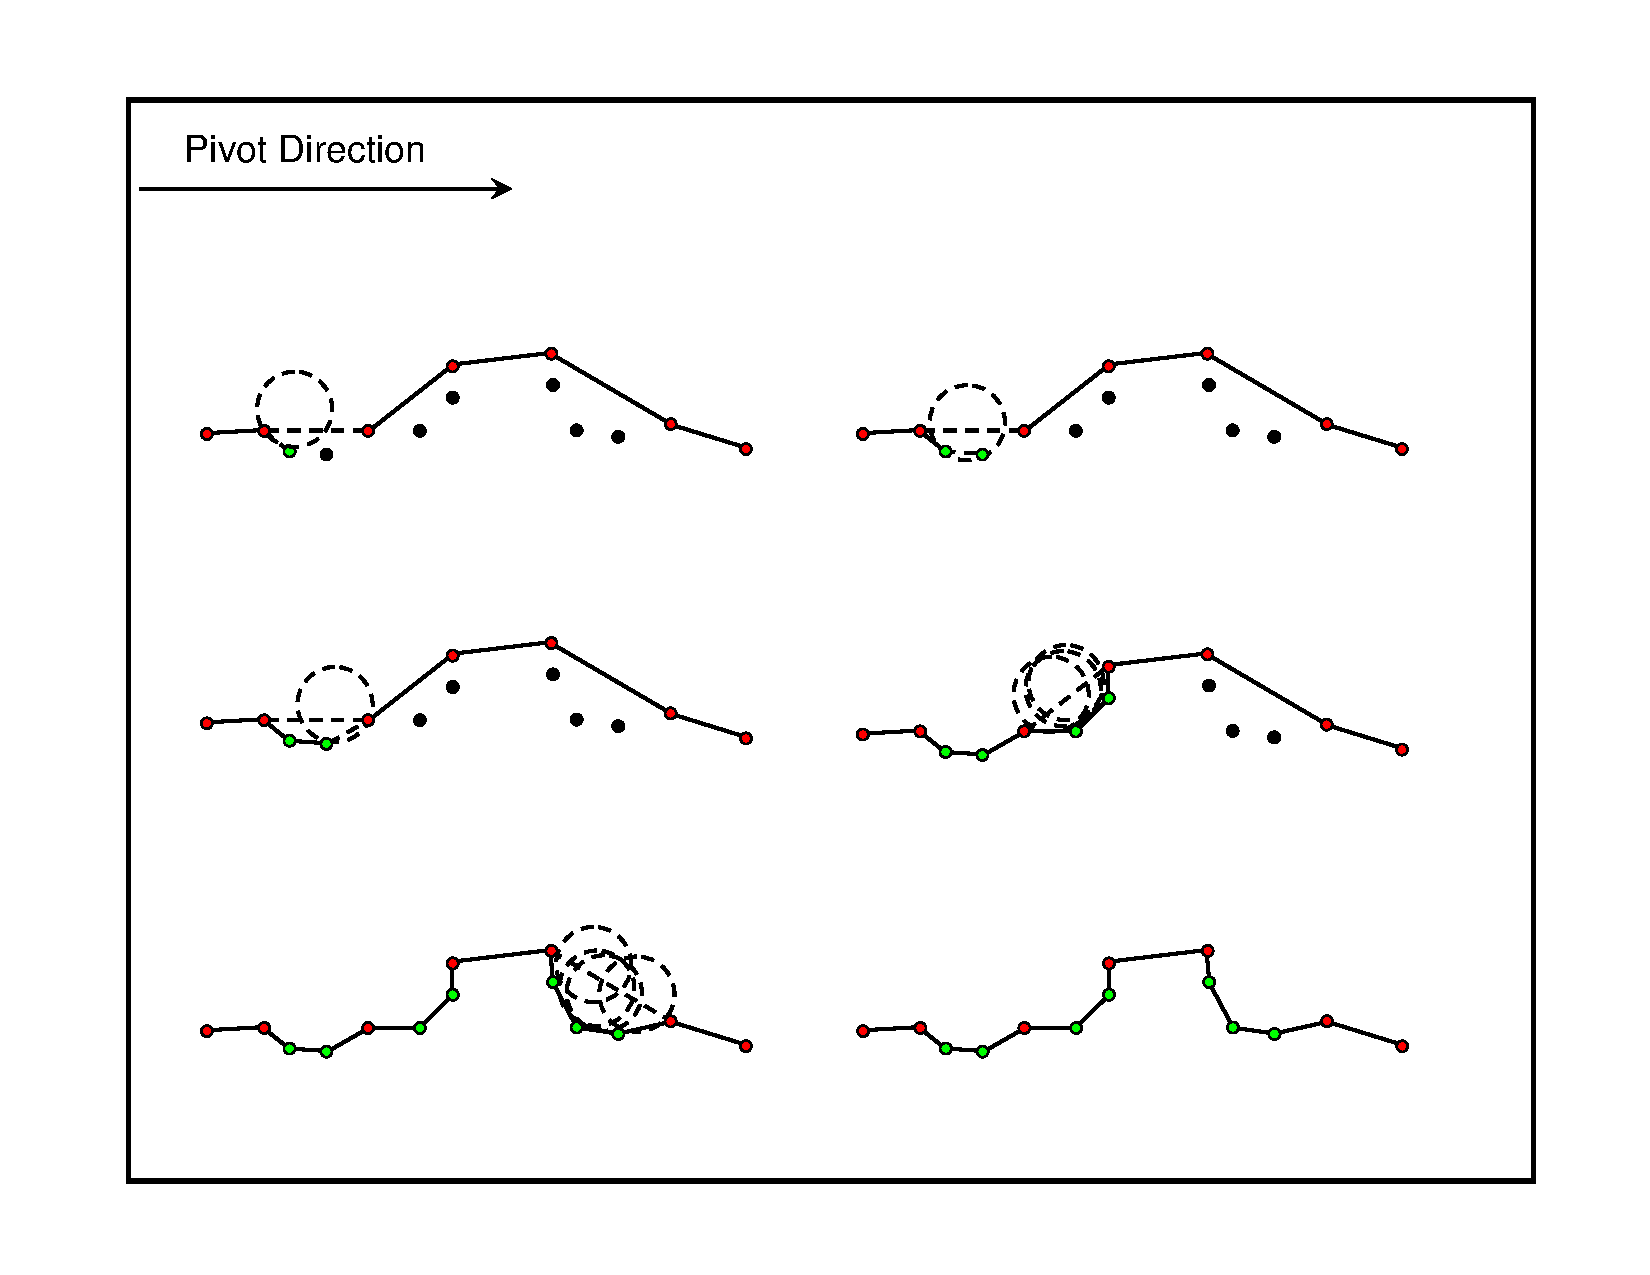
\includegraphics[width=0.8\textwidth]{BPA_refine.pdf} \\
(b)
\end{tabular}
\end{center}
\caption{Adaptive ball pivoting algorithm:
(a) Initial pivoting with a ball of radius 2$r$;
(b) Refinement with a ball of radius $r$.}
\label{fig:BPA}
\end{figure*}


The idea of the BPA is straight-forward:
pivot a ball on a starting point in the image
until it touches another data point as depicted in \Figa{BPA}.
Add the new touched
data point into an ordered list as the vertices of the contour polygon and
set it as the new pivoting point.
Keep doing this pivoting process until all data points are touched.

\section{Boundary Vectorization}
The basic idea behind the proposed framework for contour computation is as follows:
apply BPA on a selected starting point until
either the ball pivots back to the starting point 
which indicates a closed boundary is detected,
or the ball reaches a gap which means this contour is a non-closed
contour and one of the end points is reached.
Because the ball can start pivoting along either clock-wise direction 
or counter clock-wise direction,
another pivoting process at start pivoting from the other direction is conducted.
When both directions have been explored, a contour computation is done.
After this, the refinement process is carried out 
for each line segments using the same BPA algorithm.
For this refinement, the starting point is now the first end point of a line
and the stopping case is that the ball reaches the other point or it reaches a gap.

Here is more detailed description for the algorithm.
At the initial BPA stage, a relatively large radius $r$ is chosen 
as a coarse step to cover all gaps between data points.
The output of the initial BPA, $\boldsymbol{\Phi}$, 
contains an ordered list of the boundary data points $\boldsymbol{P}$ 
and their corresponding directions $\overrightarrow{\boldsymbol{R}}$ 
in which the ball $C$ starts pivoting.
The BPA refinement process applies a smaller radius, say $r' = r/2$,
to $\boldsymbol{\Phi}$ to get more accurate results, as shown in \Figb{BPA}.
For this stage, the length of each line segment formed by adjacent points is checked,
$\ell = \overline{P_0P_1}$, in $\boldsymbol{\Phi}$.
For long line segments, the BPA is applied between the two adjacent points.
When the ball reaches the second end point, a new list of ordered boundary points,
$\boldsymbol{\Phi'}$, is inserted into $\boldsymbol{\Phi}$ between $P_0$ and $P_1$.
This process continues until it finishes 
checking every adjacent point in $\boldsymbol{\Phi}$.
The refinement stops when $r'$ falls below threshold $\tau_r$.

The key parameter for the BPA algorithm to work successfully is finding
a good initial size of the ball for pivoting.
Here are some general guidances for choosing the radius. 
If a contour is known to be a closed polygon,
the initial radius should be big, e.g. the width of an image, 
to cover all gaps along the boundary.
Otherwise, if a boundary consists of sub-boundaries, 
one could select a relative small radius to start.

An example on the proposed framework is shown in \Fig{BPA_refinement}.
The initial BPA takes radius $\tau_r$ = 128,
which produced a coarse contour as shown in \Figa{BPA_refinement}.
\Figb{BPA_refinement} - \Figd{BPA_refinement} show that the contour is becoming more
accurate as the radius $\tau_r$ decreases from 32 to 2. Note that the original
image size is 1024x392 pixels as shown in \Figa{failed_case}.

\begin{figure}[htbp]
\begin{center}
\begin{tabular}{cc}
\fbox{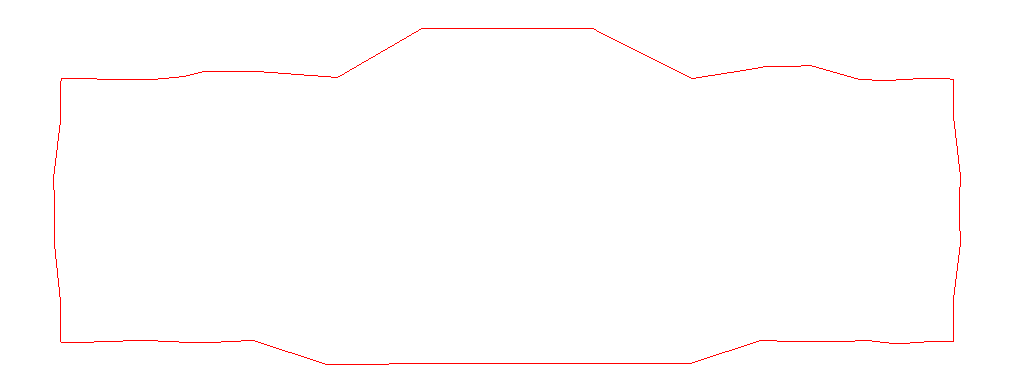
\includegraphics[width=0.45\textwidth]{global_init_refine_with_rad_128.png}} &
\fbox{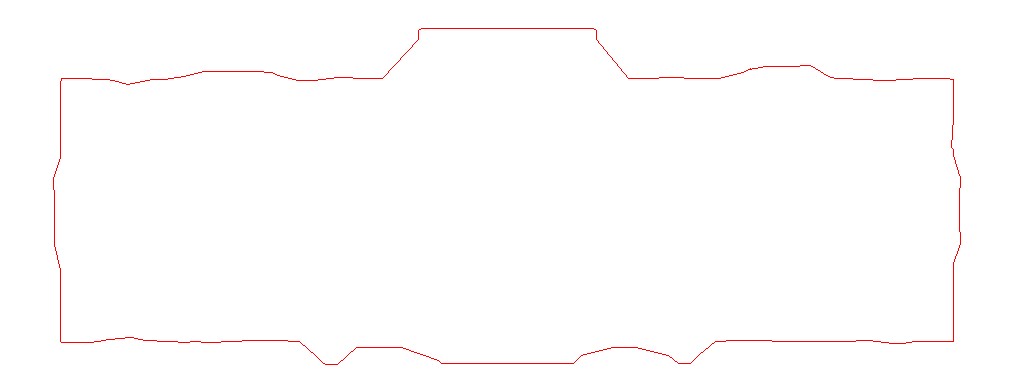
\includegraphics[width=0.45\textwidth]{global_init_refine_with_rad_32.png}} \\
(a) & (b) \\
\fbox{
\includegraphics[width=0.45\textwidth]{global_init_refine_with_rad_8.png}} &
\fbox{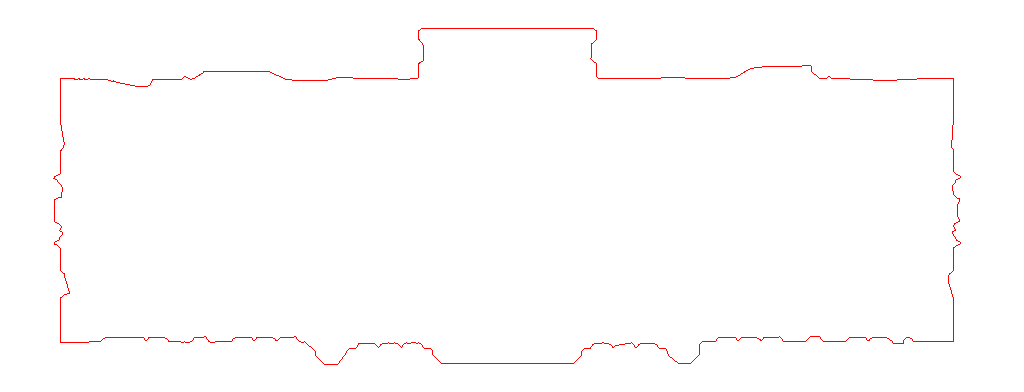
\includegraphics[width=0.45\textwidth]{global_init_refine_with_rad_1.png}} \\
(c) & (d)
\end{tabular}
\end{center}
\caption{Boundary vectorization of a binary image with (a) radius = 128
(b) radius = 32 (c) radius = 8 (d) radius = 2.}
\label{fig:BPA_refinement}
\end{figure}


\begin{figure*}[htbp]
\begin{center}
\begin{tabular}{c}
\fbox{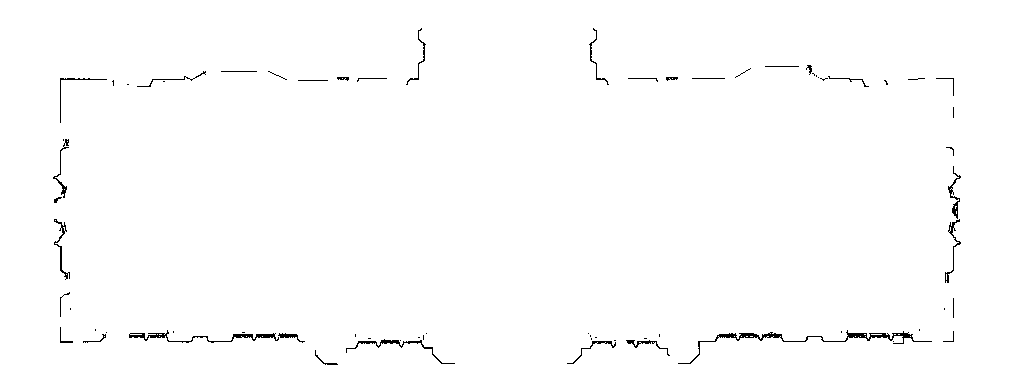
\includegraphics[width=0.7\textwidth]{failed_case.png}} \\
(a) \\
\fbox{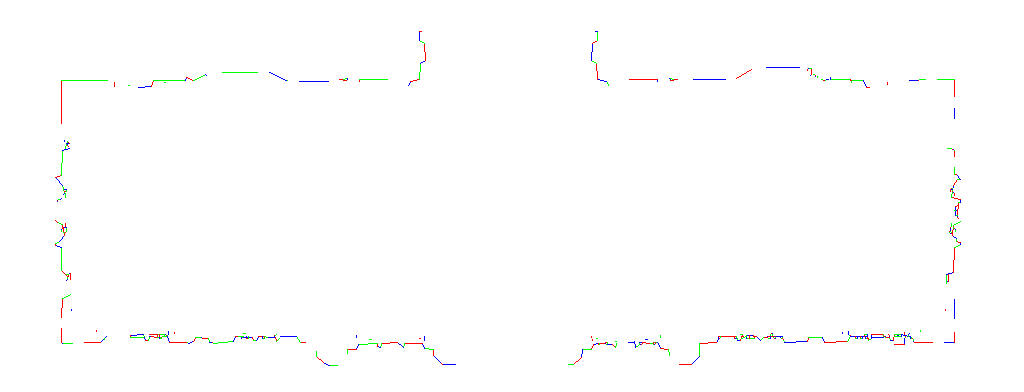
\includegraphics[width=0.7\textwidth]{failed_case_ply.png}} \\
(b) \\
\fbox{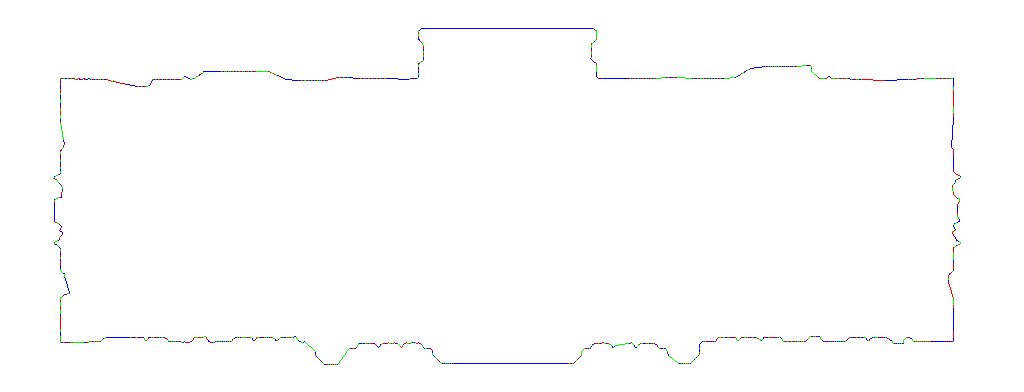
\includegraphics[width=0.7\textwidth]{failed_case_bpa.png}} \\
(c) 
\end{tabular}
\end{center}
\caption{(a) An example of binary image.
(b) The vectorization result based on DP algorithm and
(c) The vectorization result from proposed BPA algorithm.}
\label{fig:failed_case}
\end{figure*}

\begin{figure*}[htbp]
\begin{center}
\begin{tabular}{c}
\fbox{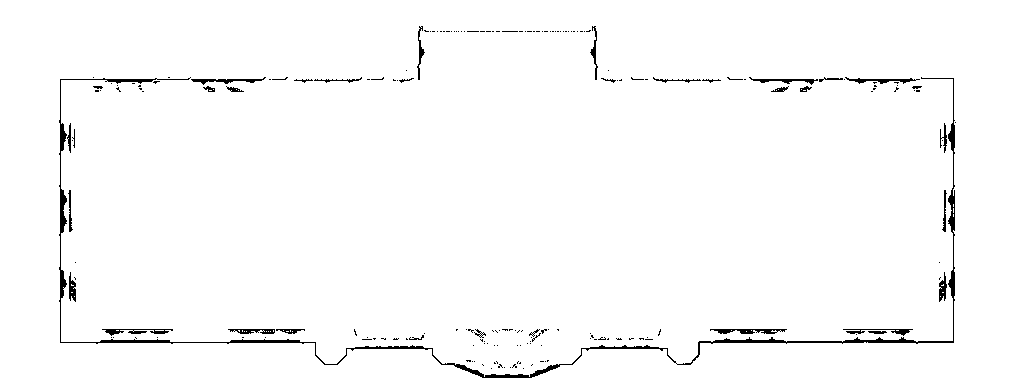
\includegraphics[width=0.7\textwidth]{aaa_image_slice_0529.png}} \\
(a) \\
\fbox{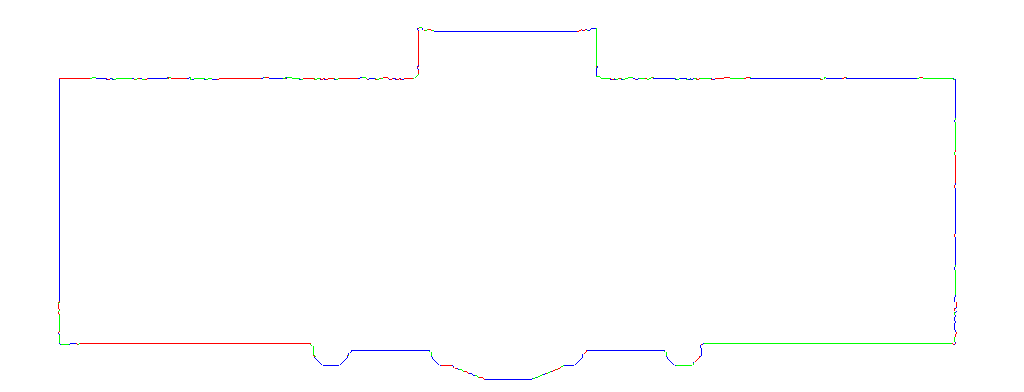
\includegraphics[width=0.7\textwidth]{bbb_image_slice_1024_392_0533_refine_with_rad_1_and_merged.png}} \\
(b) \\
\fbox{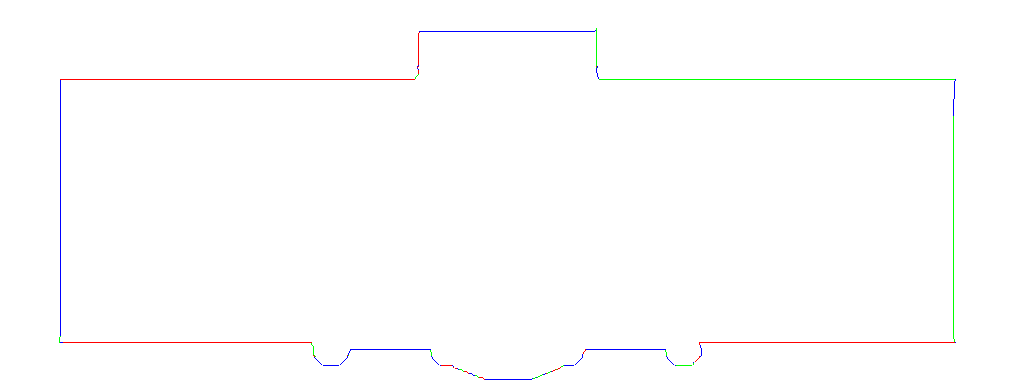
\includegraphics[width=0.7\textwidth]{bbb_image_slice_1024_392_0533_combine_HT_BPA_rad_32.png}} \\
(c)
\end{tabular}
\end{center}
\caption{Boundary vectorization of noisy binary image.
(a) the binary image to be processed.
(b) the contour computed by proposed method.
(c) the contour obtained by simplification with Hough transform.}
\label{fig:HT_BPA_figure}
\end{figure*}

\section{Contour Simplification}
\label{sec:BPA_HT}
%%% Adaptive BPA + HT %%%%

Although the proposed framework is an efficient and straightforward approach to
vectorize the contours of noisy images,
it might produce many short line segments for some special boundaries. 
An example is shown in the upper part of the contour in \Figb{HT_BPA_figure} 
(Please see this in zoomed-in mode). 
Here, each colored segment represents a contour edge.
One way to reduce the number of vertices of the polygon is to apply
the approximation polygon method in \cite{DP_AV}. 
The drawback of this method is that the topological structures, 
such as straight lines, would be lost.
To solve this issue, a Hough transform (HT) based method is proposed to replace
short line segments with long lines and potentially eliminate noisy
or outlier vertices around the boundary.

To combine the adaptive BPA with HT, 
one can first apply the HT algorithm on the original raster image $I$ 
to obtain all straight lines $\boldsymbol{L}$ and sort them by length.
The longer lines give higher confidence to the line structure of the underly images.
Then a dilation operation with 8-connected neighbors on $I$ 
can be used to get the dilation image, $I_d$.
The next step is to measure how well the lines in $\boldsymbol{L}$ match with
data in $I_d$, which determines whether a line in $\boldsymbol{L}$
should be used as a substitution or not.

If a line segment $L$ is found to be a good candidate, the next step is to
find the corresponding part of the BPA points in $\boldsymbol{\Phi}$ for
substitution. The first step is to compute the closest two points
$P_i$ and $P_j$ in $\boldsymbol{\Phi}$ to the two end points of $L$.
If the vertices in $\boldsymbol{\Phi}$ represent a polygon, they will have
a circle layout, i.e., $\boldsymbol{P} = \{ P_0,P_1,\ldots ,P_{n-1}, P_0 \}$.
Assuming $i < j$, there are two possible choices to replace
the series of the points, which are
$\boldsymbol{P_1} = \{ P_i,P_{i+1},\ldots,P_{j-1}, P_j \}$, and
$\boldsymbol{P_2} = \{ P_j,P_{j+1},\ldots,P_{i-1}, P_i \}$.
To determine which one is correct, one can compare the distance, $D$,
from the line $L$ to both set of the points $\boldsymbol{P_1}$ and
$\boldsymbol{P_2}$.
The point set with smaller $D$ is about to be substituted by the line $L$.
\begin{equation*}
D = \underset{\boldsymbol{P_1},\boldsymbol{P_2}}{\operatorname{arg\,min}}\sum{\lVert P_i - L \rVert}
\qquad P_i \in \boldsymbol{P_1} \ \text{or} \ P_i \in \boldsymbol{P_2}
\end{equation*}
where $\lVert P_i - L \rVert$ is the Euclidean distance from point $P_i$ to
line $L$.

After the integration of BPA contour with the Hough transform lines,
the beautified contour is shown in \Figc{HT_BPA_figure}.
Notice that the top part of the contour, which consisted of short line segments, 
was replaced with two long line segments.
As one can see, this process reduces the noise, simplifies the contour, 
and produces clean results for contours with straight line structures.

\begin{figure}[htbp]
\begin{center}
\begin{tabular}{ccc}
\fbox{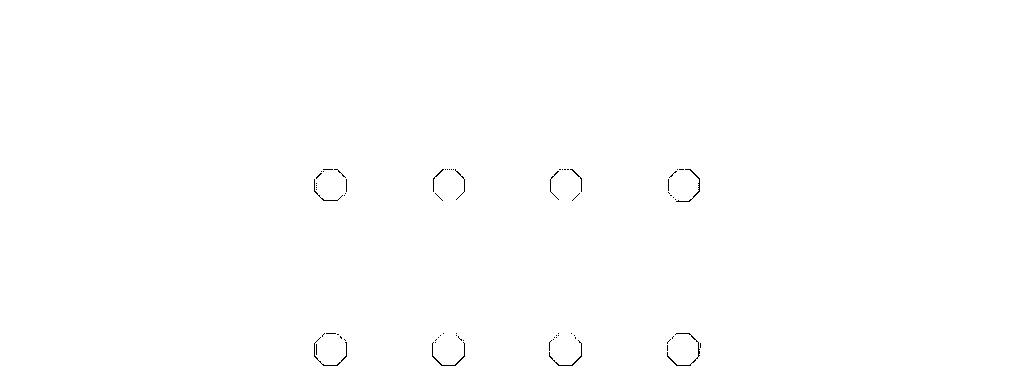
\includegraphics[width=0.3\textwidth]{image_slice_0954.png}} &
\fbox{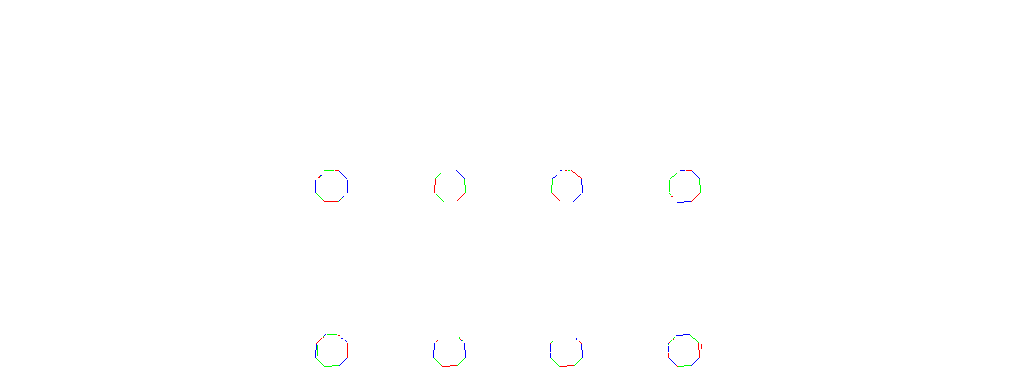
\includegraphics[width=0.3\textwidth]{image_slice_0954_ply.png}} &
\fbox{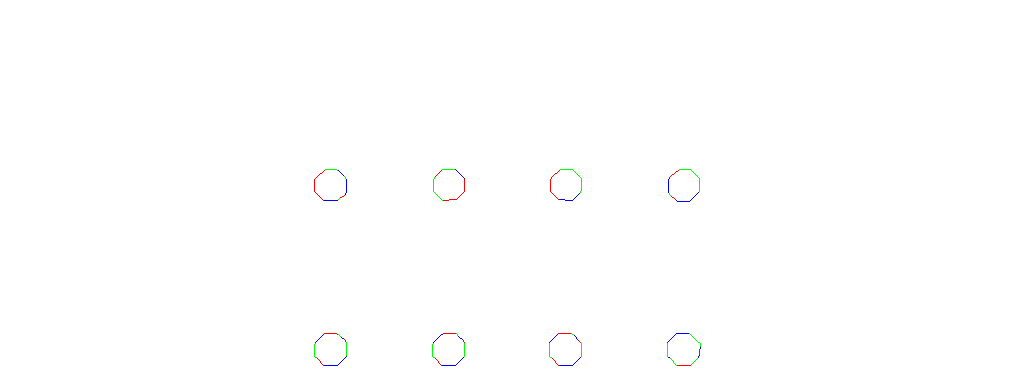
\includegraphics[width=0.3\textwidth]{image_slice_0954_rad_4_and_merged.png}} \\
(a) & (b) & (c) \\
\fbox{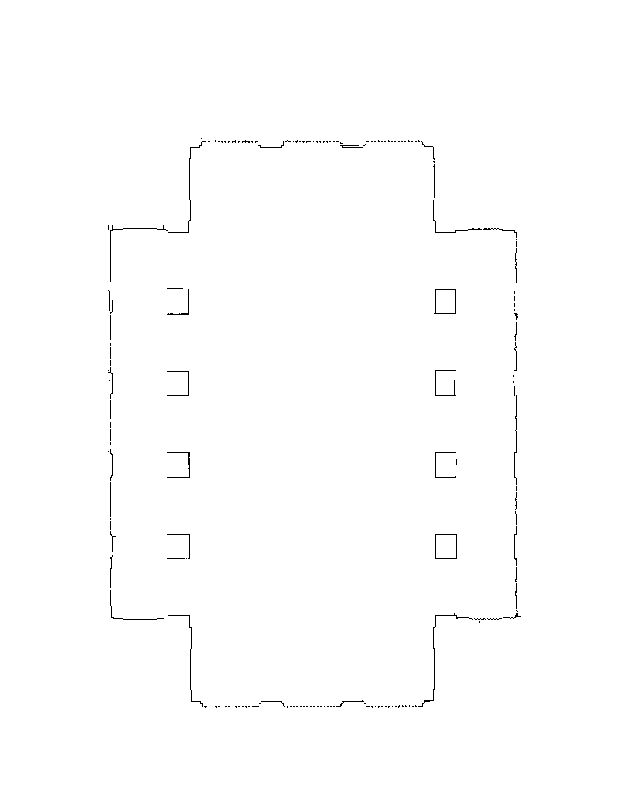
\includegraphics[width=0.3\textwidth]{image_slice_0491_p1.png}} &
\fbox{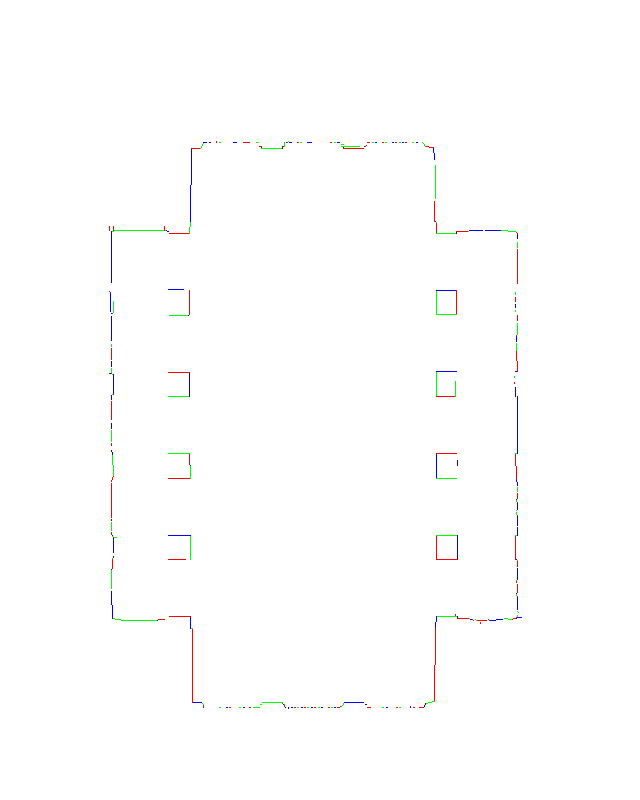
\includegraphics[width=0.3\textwidth]{image_slice_0491_p1_ply.png}} &
\fbox{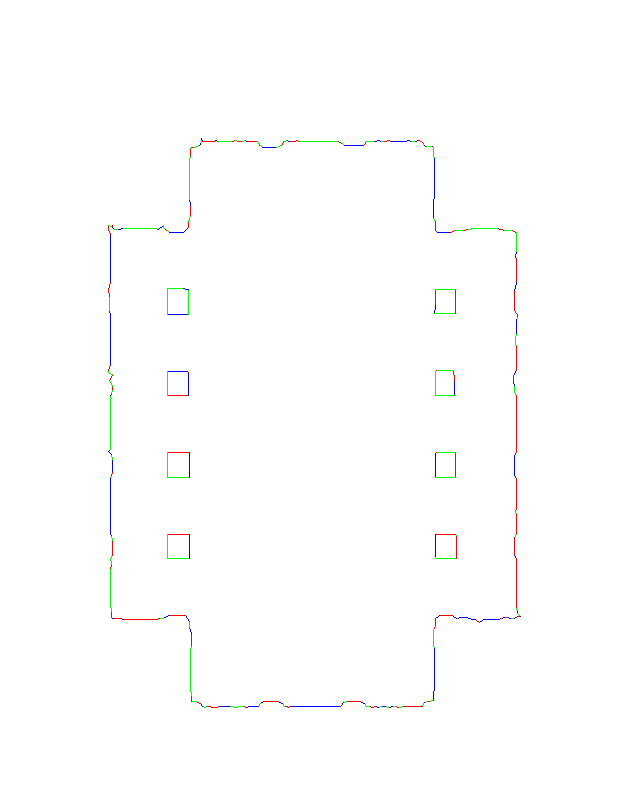
\includegraphics[width=0.3\textwidth]{image_slice_0491_p1_rad_4_and_merged.png}} \\
(d) & (e) & (f) \\
\fbox{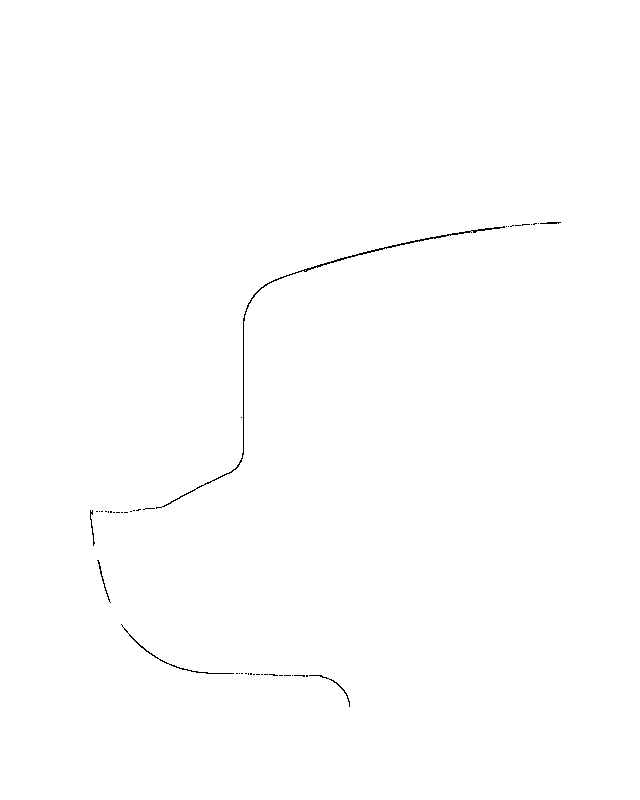
\includegraphics[width=0.3\textwidth]{image_slice_0341.png}} &
\fbox{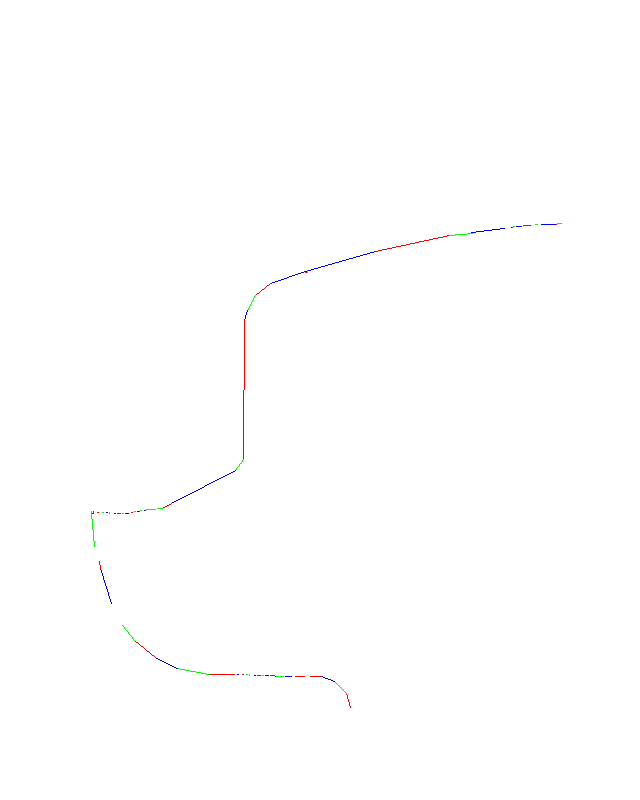
\includegraphics[width=0.3\textwidth]{image_slice_0341_ply.png}} &
\fbox{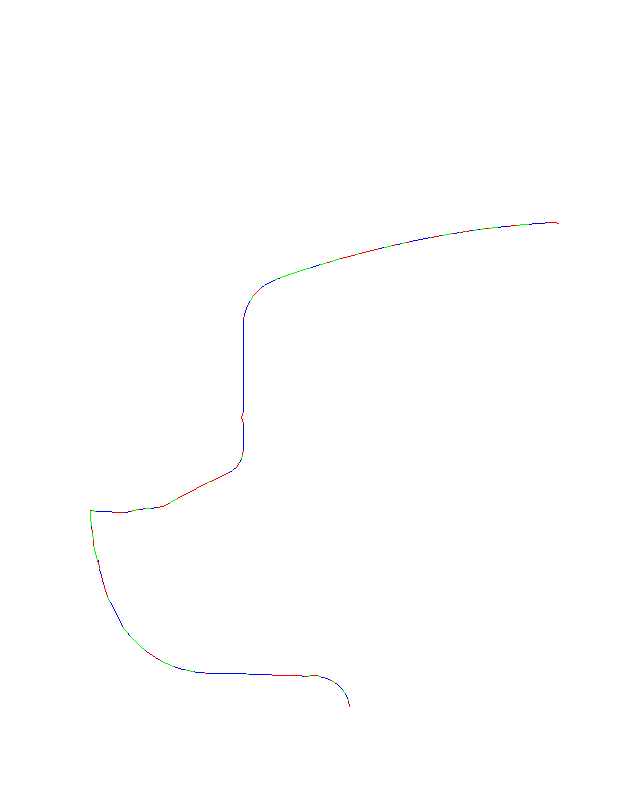
\includegraphics[width=0.3\textwidth]{image_slice_0341_rad_4_and_merged.png}} \\
(g) & (h) & (i) \\
\end{tabular}
\end{center}
\caption{
More experimental results: (a), (d) and (g) show the original noisy binary images.
(b), (e) and (h) show the vectorization results from DP algorithm.
(c), (f) and (i) show the vectorization results from proposed algorithm.}
\label{fig:results}
\end{figure}

In addition to the results shown in \Fig{failed_case} and \Fig{HT_BPA_figure}, more
experimental results are shown in \Fig{results}. In the first row of \Fig{results},
the input image is of size 1024x392 and contains multiple contours.
In the second row, the input image is 800x640 and contains nested contours.
In the third row, the input image is 800x640 and contains a curved contour.
As one can see, the proposed framework can handle all the cases properly 
and fill the holes as expected, which outperformed the standard DP algorithm.


\begin{figure}[htbp]
\begin{center}
\begin{tabular}{c}
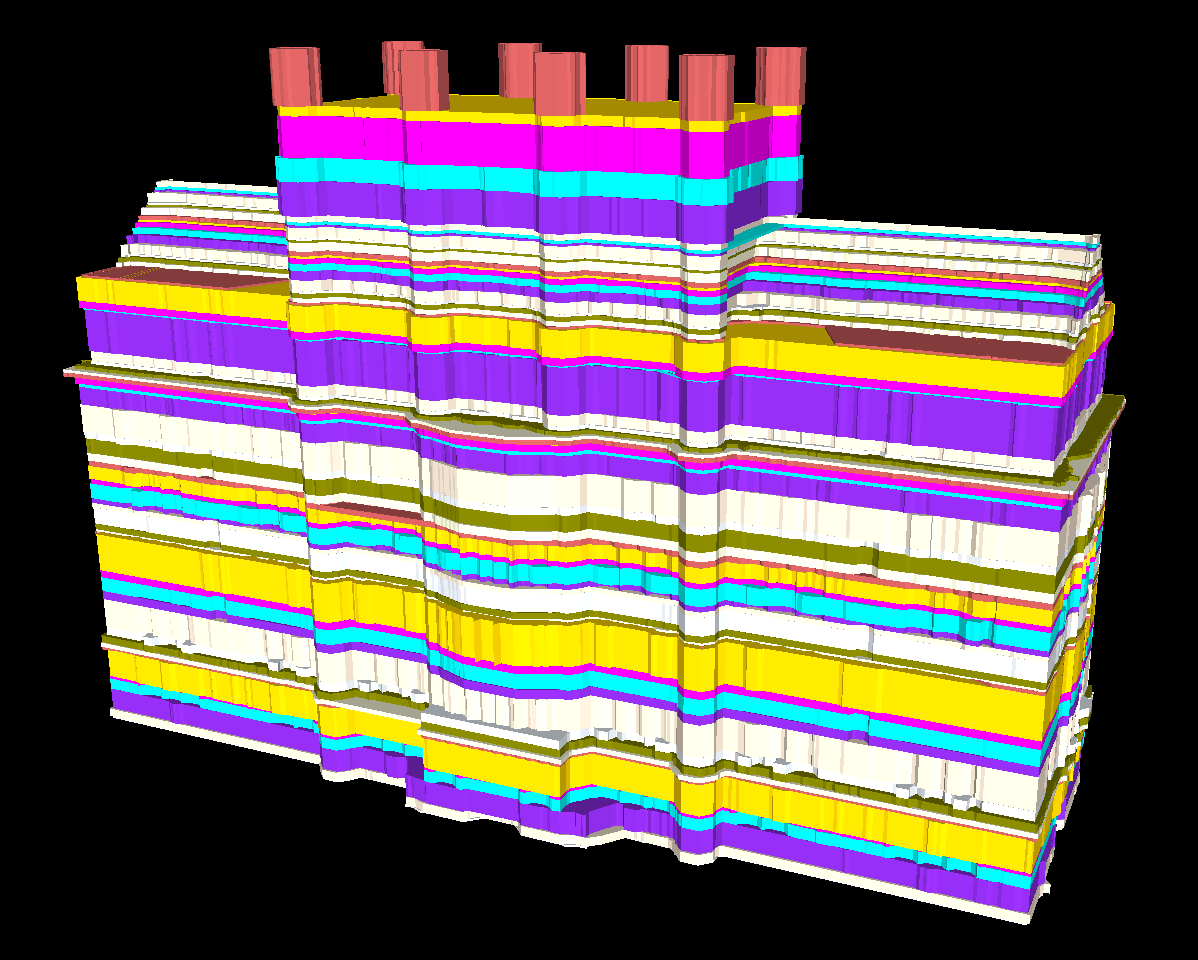
\includegraphics[width=0.8\textwidth]{notaper_8_4.png}
\end{tabular}
\end{center}
\caption{ The reconstructed model based on extrusion operation on keyslices. }
\label{fig:DXF_notaper_model}
\end{figure}

\newchapt{Tapered Structure Detection}{chapt6}{Tapered Structure Detection}

After the keyslices are detected and vectorized, the contours of
$N_K = \{I_{i}, i = 0, ..., K \}$ keyslices are used to represent
the building based on the extrusion operation.
That is, the space between each pair of keyslices, say $I_{i}$ and $I_{j}$,
can be interpolated by the lower keyslice, e.g., $I_{i}$ in this case.
This is valid due to the similarity between the intermediate slices
and the keyslice $I_{i}$.
By modeling a building using this series of keyslices $N_K$, we
significantly reduce the polygon count for urban buildings. 
An example of the reconstructed model is shown in \Fig{DXF_notaper_model}.
This helps make possible 3D web-based applications such as 3D city navigation.

In addition to the extrusion operation, we can further improve the model
and reduce the model size by observing that part of the keyslice images
belong to the same tapered structure, as demonstrated in \Fig{DXF_top}.
\Figa{DXF_top} shows the roof structure
of the reconstructed model based on a keyslice image extrusion operation with
almost half of the keyslice images dedicated to the structure.
After inferring the tapered structure, \Figb{DXF_top} shows the improvement
of the modeling, which is much smoother than the previous model.
In addition, the keyslices needed to represent the building, and its
associated storage, are reduced almost in half.

\begin{figure}[htbp]
\begin{center}
\begin{tabular}{c}
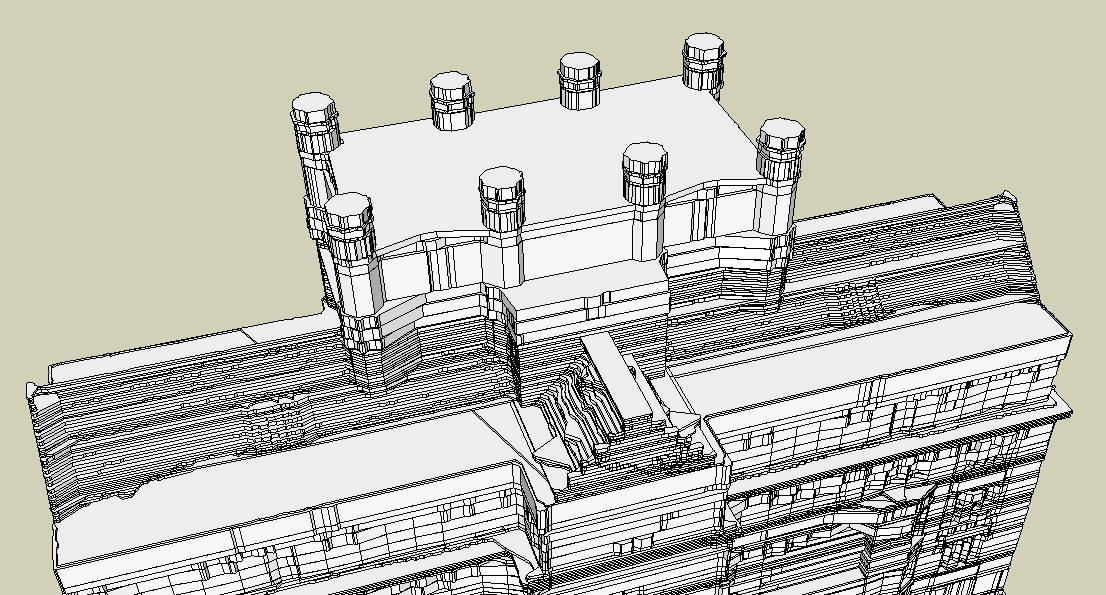
\includegraphics[width=0.7\textwidth]{extrude_1.png} \\
(a) \\
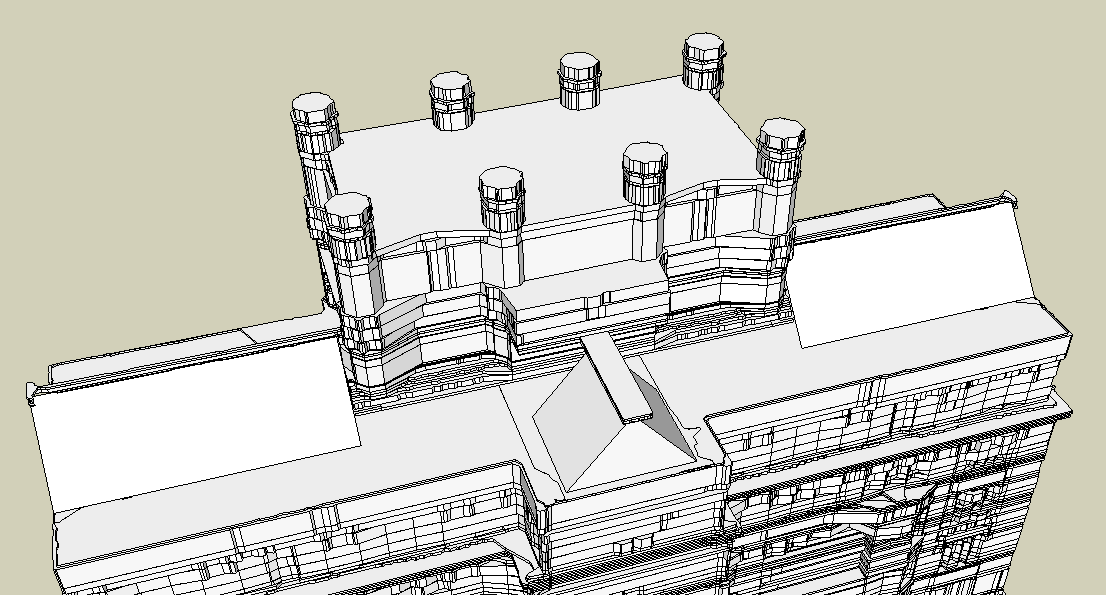
\includegraphics[width=0.7\textwidth]{extrude_2.png} \\
(b)
\end{tabular}
\end{center}
\caption{The top view of the 3D building shown (a) without tapered structures
and (b) with tapered structures.}
\label{fig:DXF_top}
\end{figure}

\section{Inferring Taper Structure}
\label{sec:tsd}

The difficulty in inferring tapered structures is tied to the complexity of
the building structure itself.
Let's assume that the height range for the roof structure is
$H_R = [H_{lo}, H_{hi}]$.
If this is the only existing structure between $H_R$, it is simple and
straight-forward to detect and infer this part.
However, for some complicated structures, such as a mixed layout
of tapered and extruded structures, as depicted in \Fig{taper_seg},
some special treatment is needed to obtain the desired results.
Our approach is based on the divide-and-conquer strategy:
the whole structure $\boldsymbol{U}$ is segmented into independent
sub-structure units, $U_0, U_1, \ldots, U_N$.
Any sub-structure unit $U_i$ is constrained to contain a unique structure,
i.e., either a tapered or an extruded one.
Once each unit $U_i$ is inferred, the whole structure can be modeled by a
union operation of these sub-structures, i.e.,
$\boldsymbol{U} = \bigcup{U_i\{ i = 1,\ldots,N\}}$.
Before segmentation, the potential height ranges $H_R$ containing the tapered
structures must be computed.
This can be done by checking the frequency of the keyslice images.
The structure containing tapered sub-structures will show a wide and uniform
distribution of keyslice images.
This is a very useful clue for $H_R$ detection.

\begin{figure}[htbp]
\begin{center}
\begin{tabular}{c}
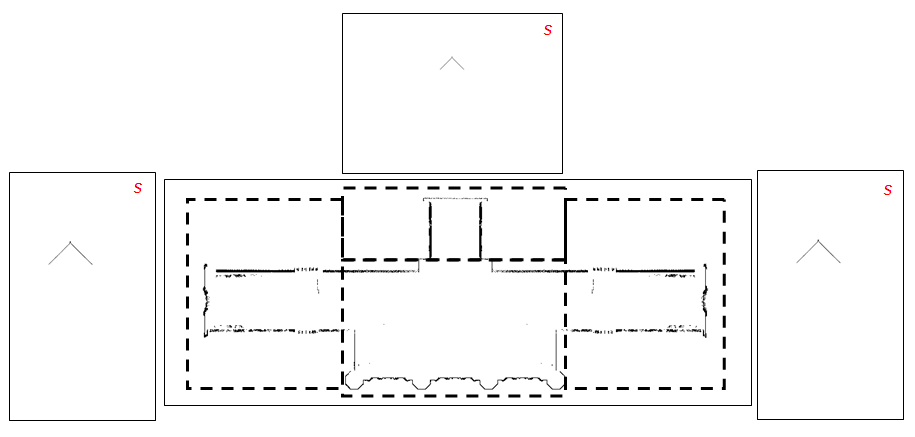
\includegraphics[width=0.8\textwidth]{extrude_3.png} \\
\end{tabular}
\end{center}
\caption{The top 2D slice of the 3D building. }
\label{fig:taper_seg}
\end{figure}

Once the potential height ranges $H_R$ is obtained, the next step is to
segment the whole structure $\boldsymbol{U}$ between $H_R$ into sub-structures,
$U_i, \; i = 0,\ldots,N$.
This is again done by applying the similarity measurement to sliced images
from orthogonal directions.
As before, the 3D data points inside the range of $H_R$ are projected
along both left-right ($X$ axis) and face-inside ($Z$ axis) directions.
Then, the keyslice detection is carried out based on the Hausdorff distance
similarity measurement for both directions.
These keyslices will segment the structure in $H_R$ into subunits of
$U_0, U_1, \ldots, U_N$.

For each subunit $U_i$, we must determine 
whether it represents an extruded or a tapered structure.
This is done by checking in keyslice image $I_k$ of $U_i$ whether there exists
a pattern where two lines intersect with some appropriate angle.
If such a pattern exists in $I_k$, such as the images marked with red $s$ in
\Fig{taper_seg}, the unit $U_i$ is considered to be a tapered sub-structure unit.
Otherwise, $U_i$ is treated as an extruded sub-structure unit.
If $U_i$ is an extruded unit, its contours from the $y-$ axis are vectorized
and is ready for the union operation to obtain $\boldsymbol{U}$.
On the other hand, if $U_i$ is a tapered unit, the bottom and top position
have to be computed so that it can be reconstructed.
To do this, all line segments $\boldsymbol{L}$ in $U_i$ are computed using
the Hough Transform and the intersection point $P_0$ of $\boldsymbol{L}$
indicates the top position of the tapered unit.
The other end points $P_i$ of $\boldsymbol{L}$ are also computed to infer
the bottom shape and position. 
The model enhanced by taper operation is shown in \Fig{DXF_taper_model}.

\begin{figure}[htbp]
\begin{center}
\begin{tabular}{c}
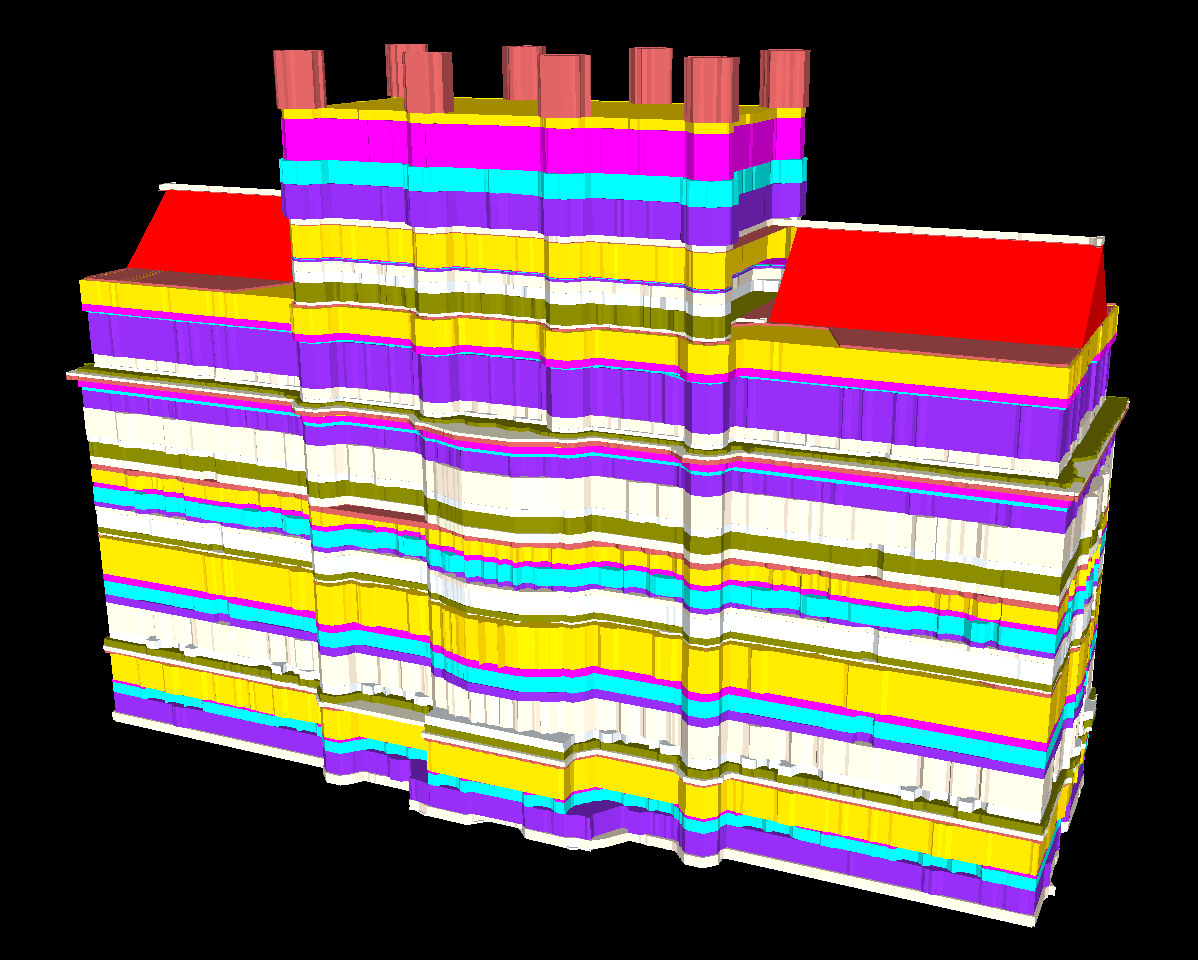
\includegraphics[width=0.8\textwidth]{taper_8_4.png}
\end{tabular}
\end{center}
\caption{ The reconstructed model enhanced by taper operation on roof structure. }
\label{fig:DXF_taper_model}
\end{figure}

\section{Taper-to-point Structure Inference}
\label{sec:tsd_ttp}
The approach we described and illustrated in the previous sections can only be
applied on the inference of taper-to-line structure. 
In addition to this, there is another
type of tapered structure, i.e. taper-to-point structure which appears frequently in 
Gothic architecture, such as churches.
Unlike the taper-to-line, this type of taper structures are not able to be inferred 
through the extruded structure from the orthogonal directions.
However, a nice characteristic of this type of taper structure is that
the vertices of the base geometry converge to a point, which is good clue for inference.
\Fig{DXF_taper_both} shows a synthetic data model consists of both taper-to-point (left)
and taper-to-line (right) structures. 

\begin{figure}[htbp]
\begin{center}
\begin{tabular}{c}
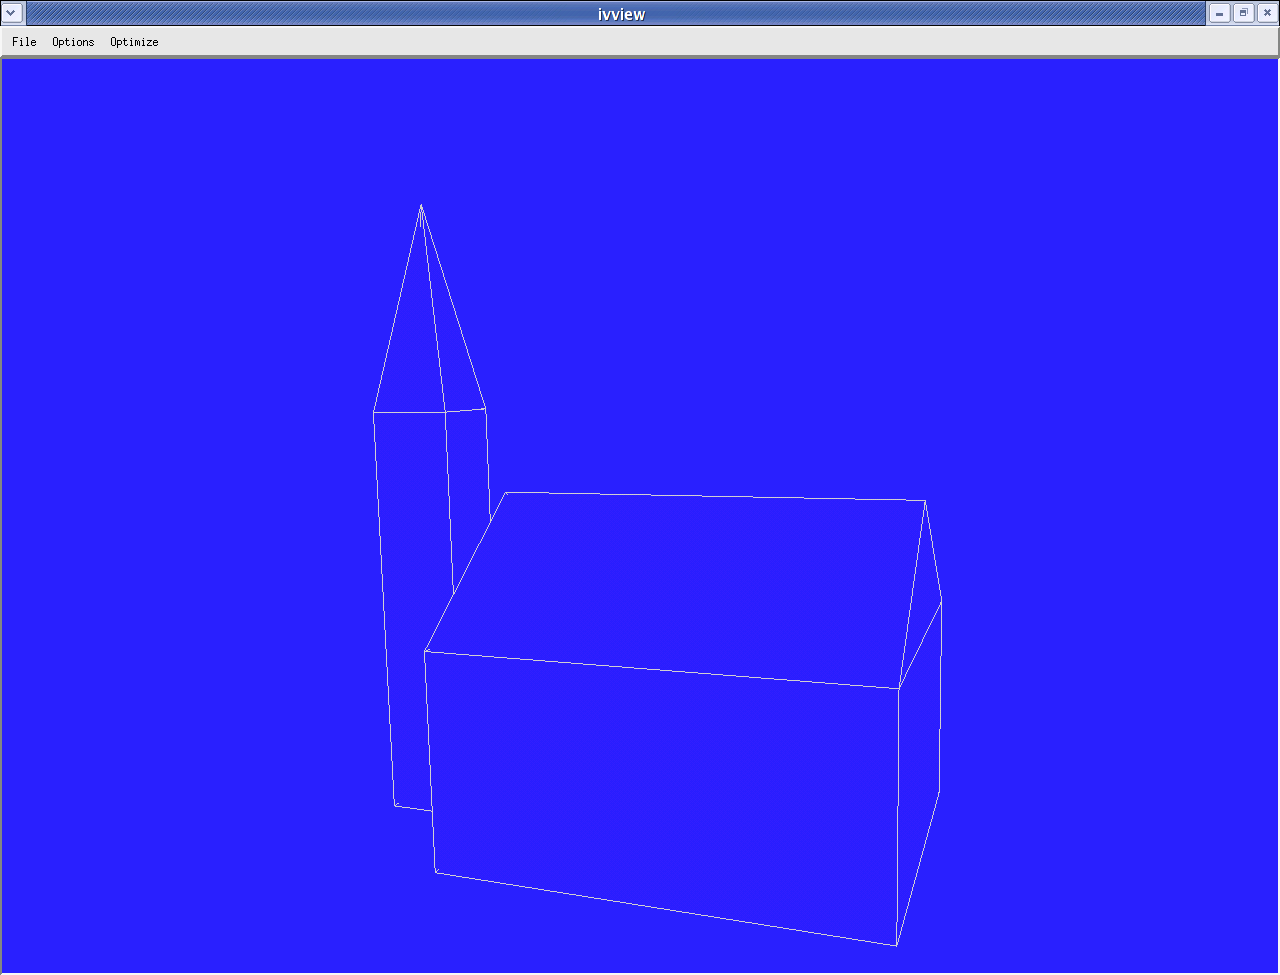
\includegraphics[width=0.8\textwidth]{taper_both_syn.png}
\end{tabular}
\end{center}
\caption{ The synthetic model consists of taper-to-point and taper-to-line structures. }
\label{fig:DXF_taper_both}
\end{figure}

Without loss of generality, we assume that the sliced images of this special structure
can be vectorized by a closed polygon.
Let $S_i$, $S_j$ be two consecutive sliced images and $S_i$
has a smaller boundary than $S_j$. Based on this special structure, $S_i$ will be growing up
to cover $S_j$ by iterative dilation operations. By doing this, we can quickly locate the
bottom and top (a small region representing a point) slices of this special geometry
structure and therefore reconstruct this sub-model using these two slices.
The difference between this structure and the structure of tapering to a line is whether
$S_i$ and $S_j$ have any overlapping or common parts, which is easy to check.




\newchapt{Algorithm Analysis}{chapt7}{Algorithm Analysis}

%%%%%%%%%%%%%%%%%%%%%%%%%%%%%%%%
%%%%%%  Algorithm Analsysis  %%%
%%%%%%%%%%%%%%%%%%%%%%%%%%%%%%%%
\section{Algorithm Analysis}
\label{sec:PE_AA}

\begin{algorithm}
\caption{The Adaptive Hough Transform Algorithm}
\label{alg.AHT}
\begin{algorithmic}[1]
\Procedure {AHTA}{$I$, $\boldsymbol{L}$}
\While {$true$}
\State $\bigcup{(\rho, \theta)} \leftarrow HT (I)$  \Comment{regular hough transform to get a set of lines}
\State $n \leftarrow 0 $
\For {each $(\rho, \theta) \in \bigcup{(\rho, \theta)} $}
     \State $c \leftarrow num(I, \rho, \theta)$  \Comment{compute \# of points falling onto line ($\rho, \theta$)}
     \If {$n < c$}
         \State $n \leftarrow c$
         \State $\rho_{max} \leftarrow \rho$
         \State $\theta_{max} \leftarrow \theta$
     \EndIf
\EndFor
\If {$n > \epsilon $}   \Comment{ sanity check for the line ($\rho_{max}, \theta_{max}$) }
\State $\boldsymbol{L} \leftarrow (\rho_{max}, \theta_{max})$
\State $update(I, \rho_{max}, \theta_{max})$ \Comment{ remove points falling onto line ($\rho_{max}, \theta_{max}$)}
\Else
\State $break$
\EndIf
\If {$\omega(I) < \epsilon$} \Comment{ check how many points left }
\State $break$
\EndIf
\EndWhile
\EndProcedure
\end{algorithmic}
\end{algorithm}

The Adaptive Hough Transform (AHT) algorithm stems from the original Hough transform algorithm.
The function $HT()$ is just a regular Hough Transform (HT), which is $O(L)$ for line detection. 
Here $L$ is the data point in 2D image.  The computation of the number of points covered by 
each line  ($\rho, \theta$) detected by $HT$ is of $O(L)$ complexity.
The sanity check and image update function $update()$ is most of query and comparison operation, which is
$O(1)$ complexity. Because we are dealing with bounded number of data points, and the data points
on the longest line of each iteration are removed for each iteration, the AHT will quickly converge.
Because the 3D point cloud data has been projected to 2D image, the worst case for 3D data points is
$O(N)$, where $N$ is the total number of 3D points.

The space complexity of AHT algorithm is bounded by the space complexity of the $HT()$ algorithm. 
Because we are only working on line detection of 2D images, the space complexity is $O(N_\rho * N_\theta)$, 
where $N_\rho$ and $N_\theta$ represents the number of bins for quantizing the value of $\rho$
and $\theta$ respectively. For example, for a image of size 300x400, if we quantize the length $\rho$
with one bin for each pixel, the $N_\rho$ would be 500. Also, if we quantize the the angle with one
bin for a degree, the $N_\theta$ would be 180. Based on this, the space complexity for this example 
can be easily obtained. The precise of the Hough transform algorithm is depend on the quantization 
of the parameters $\rho$ and $\theta$. The more bins are used for quantization, the more precise the
results will be, which implies more space are needed for the algorithm.


\begin{algorithm}
\caption{The 2D Adaptive Ball-Pivot Algorithm}
\label{alg.ABPA}
\begin{algorithmic}[1]
\Procedure {ABPA}{$I$, $\boldsymbol{L}$}
\State $L \leftarrow \emptyset$
\State $P, P_0 \leftarrow S(I) $ \Comment{compute the $seed$ point assigned to $P$ and $P_0$}
\State $r \leftarrow W$ \Comment{initialize radius $r$ with a large value $W$}
\While {$true$}  \Comment{initial BPA stage}
   \State $append(L, P)$ 
   \State $P_i \leftarrow BPA(P, I, r)$ \Comment{regular 2D BPA}
   \If { $P_i = P_0 $ } 
      \State $break$ \Comment { complete the initial BPA }
   \EndIf
   \State $P \leftarrow P_i$ \Comment { find a new vertex $P$ for the contour $L$}
\EndWhile

\State $r \leftarrow W'$ \Comment{a smaller radius $W'$ for refinement}
\While {$r > \epsilon$} \Comment {iterative BPA refinement}
   \For { each line $\overline{P_iP_j} \in \boldsymbol{L} $}
      \State $L' \leftarrow \emptyset$
      \State $P \leftarrow P_i$
      \While {$true$}
         \State $append(L', P)$ \Comment{construct a sub contour $L'$}
         \State $P_k \leftarrow BPA(P, I, r)$ 
	 \If { $P_k = P_j $ } \Comment{stop when reaching the other point}
	    \State $substitute(L, P_i, P_j, L')$ \Comment{refine $\overline{P_iP_j}$ with $L'$}
	    \State $break$
	 \ElsIf { $isGap(L', P_k)$ }  \Comment{stop when reaching a gap}
	    \State $break$
	 \EndIf
	 \State $P \leftarrow P_k$ \Comment { find a new vertex $P$ for $L'$}
      \EndWhile
   \EndFor
   \State $r \leftarrow r/2$  \Comment{reduce the radius for next iteration}
\EndWhile
\EndProcedure
\end{algorithmic}
\end{algorithm}

The 2D adaptive ball-pivot algorithm (ABPA) is summarized in Algorithm \ref{alg.ABPA}. 
The seed computation $S()$ is to randomly pick up a good starting point, which
is only $O(1)$ complexity. The $append()$ function is to concatenate the control 
points, which is only $O(1)$ complexity. The regular 2D ball-pivot algorithm, $BPA()$,
carries out the geometry computation on each control point based on the size of the
radius of the ball or circle. Basically, for each pivoting of the ball, the area 
in the image covered by this pivoting is checked. If there is a data point contained
by this area, the pivoting ends for this control point. 
The complexity for computing the whole potential pivoting area is $O(n)$???, the
complexity to pick up the minimum angle of the pivoting is $O(1)$, therefore, the 
complexity for the whole 2D $BPA()$ is $O(n)$. 

For the refinement process, each line $\overline{P_iP_j}$ of the boundary generated
in the previous iteration is checked using the same algorithm in $BPA()$. This only
takes $O(n)$ complexity. The $substitute()$ and $isGap()$ function is just to insert
a extra point or a simple algebra computation, the complexity for both operations is 
$O(1)$, Because the round of the refinement process is bounded by a predefined constant 
number, say $c$, the complexity of this refinement is also bounded by $O(c*n) = O(n)$. 

The implementation of the ABPA uses O(m) memory space, where m is the size of the 2D image.
This complexity includes the enqueue/dequeue the control points of the boundary, the 
pivoting geometry computation and the $substitute()$ and $isGap()$ computations. Since
the user can control the size of slices, memory requirements can be tailored to the
available hardware. 

\begin{algorithm}
\caption{The Keyslice Detection Algorithm}
\label{alg.KSD}
\begin{algorithmic}[1]
\Procedure {Hausdorff}{$I$, $N$}
  \State $K \leftarrow \emptyset$  \Comment{vector to store the indexes of keyslices}
  \State $I_r \leftarrow I_0$
  \For { $i \leftarrow 1, N-1 $}
    \State $d_1 \leftarrow dis(I_r, I_i) $
    \State $d_2 \leftarrow dis(I_i, I_r) $
    \State $d_{HD} \leftarrow avg(d_1, d_2) $ \Comment {average Hausdorff distance}
    \If { $d_{HD} > \epsilon $}
       \State $I_r \leftarrow I_i$  \Comment{update the reference image}
       \State $ append(K, i) $
    \EndIf
  \EndFor
  \State \textbf{return} $K$
\EndProcedure

\Procedure {Curvature}{$I$, $N$}
  \State $K \leftarrow \emptyset$  \Comment{vector to store the indexes of keyslices}
  \State $V \leftarrow 0$ \Comment {initialize the counter to 0}
  \For { $i \leftarrow 0, N-1 $}
     \State $\bigcup{C} \leftarrow curv(I_i)$ \Comment{curvature computation on image $I_i$}
     \State $\bigcup{c} \leftarrow mapping(\bigcup{C}) $ \Comment{mapping the curvature to indexes}
     \For {each $c \in \bigcup{c}$ }
        \State $V(c) \leftarrow V(c) + 1$ \Comment{increase the number of curvature observed}
     \EndFor
  \EndFor
  \For { each $c \in \bigcup{c}$ }
     \If { $V(c) > \epsilon $}  \Comment {validate the curvatures}
	\State $append(K, c)$
     \EndIf
  \EndFor
  \State \textbf{return} $K$
\EndProcedure

\Procedure {KSDA}{$I$, $S$}
\State $K_1 \leftarrow Hausdorff(I, S)$ \Comment{keyslices computed by Hausdorff distance}
\State $K_2 \leftarrow Curvature(I, S)$ \Comment{keyslices computed by Curvature}
\State $K \leftarrow merge(K_1, K_2)$
\EndProcedure
\end{algorithmic}
\end{algorithm}

The idea of keyslice detection is described in Algorithm \ref{alg.KSD}. 
Essentially, the algorithm consists of two independent procedures. 
The function $Hausdorff()$ is conducting Hausdorff distance based keyslice
detection. A lookup table $t$ is created for the implementation of $Hausdorff()$. 
This lookup table is created by computing for each pixel $p$ in the reference image $I_r$,
how far is $p$ to the nearest data point. If $p$ itself is a data point, the distance is 0.
The complexity of constructing $t$ bounded by $O(w*h)$, where $w$ and $h$ are the image
width and height respectively. Once $t$ is computed, the function $dis()$ is only
$O(1)$ complexity which basically doing queuing from $t$. Therefore, the function $Hausdorff()$
takes $O(n)$ complexity. 
For procedure $Curvature()$, the function $curv()$ which computes curvatures
in the orthogonal direction is of $O(n)$ complexity. The $mapping()$ function and
the remaining steps mainly consists of couple of algebra computation, which takes $O(1)$ complexity. 
Therefore the procedure $Curvature()$ is of $O(n)$. Overall, the algorithm $KSDA()$ takes
$O(n)$ computation complexity for keyslice detection. 

For the space complexity, the keyslice detection algorithm is similar to adaptive ball-pivot
algorithm and uses $O(m)$ memory for computation. Again, the memory usage can be tailored to 
available hardware based on user settings.


\newchapt{Performance Evaluation}{chapt8}{Performance Evaluation}


%%%%%%%%%%%%%%%%%%%%%%%%%%%%%%%%
%%%%%%   Experimental Results%%%
%%%%%%%%%%%%%%%%%%%%%%%%%%%%%%%%
\section{Experimental Results}
\label{sec:IR_OUT}

The results of the extrusion and tapered structures computation,
together with keyslice image vectorization, are stored in the 2D
image coordinate system. To generate the final 3D model, these
data need to be transformed back into the 3D world coordinate system.
Let $P(x,y)$ be a point in the 2D image coordinate system, and let $P'(x,y,z)$
be the 3D world coordinate of $P$, where $y$ is the depth coordinate.
For all points in the same contour, the points lie in the same plane and
hence have the same value of $y$.
The equation for transforming $P$ back to $P'$ is a reverse transformation
of $\boldsymbol{T_0}$ in \Eq{image_slicing}:
\begin{equation}
[\,x^{3D},\; y^{3D},\; z^{3D}\,]^T = [\,\eta\cdot x^{2D} + X_{MIN},\; \zeta + Y_{MIN},\; \eta\cdot z^{2D} + Z_{MIN}\,]^T
\label{eq:ir2dxf}
\end{equation}
where $\eta=1/\omega$ and $\zeta=\kappa\cdot\delta$. Here, $\kappa$ is the
index of the 2D slice and $\delta$ is the height of a slab, as described
in \Sec{image_slicing}.
\Figd{IR_2_DXF} shows an exterior 3D model generated by the above
transformation.

\begin{figure*}[htbp]
\begin{center}
\begin{tabular}{c}
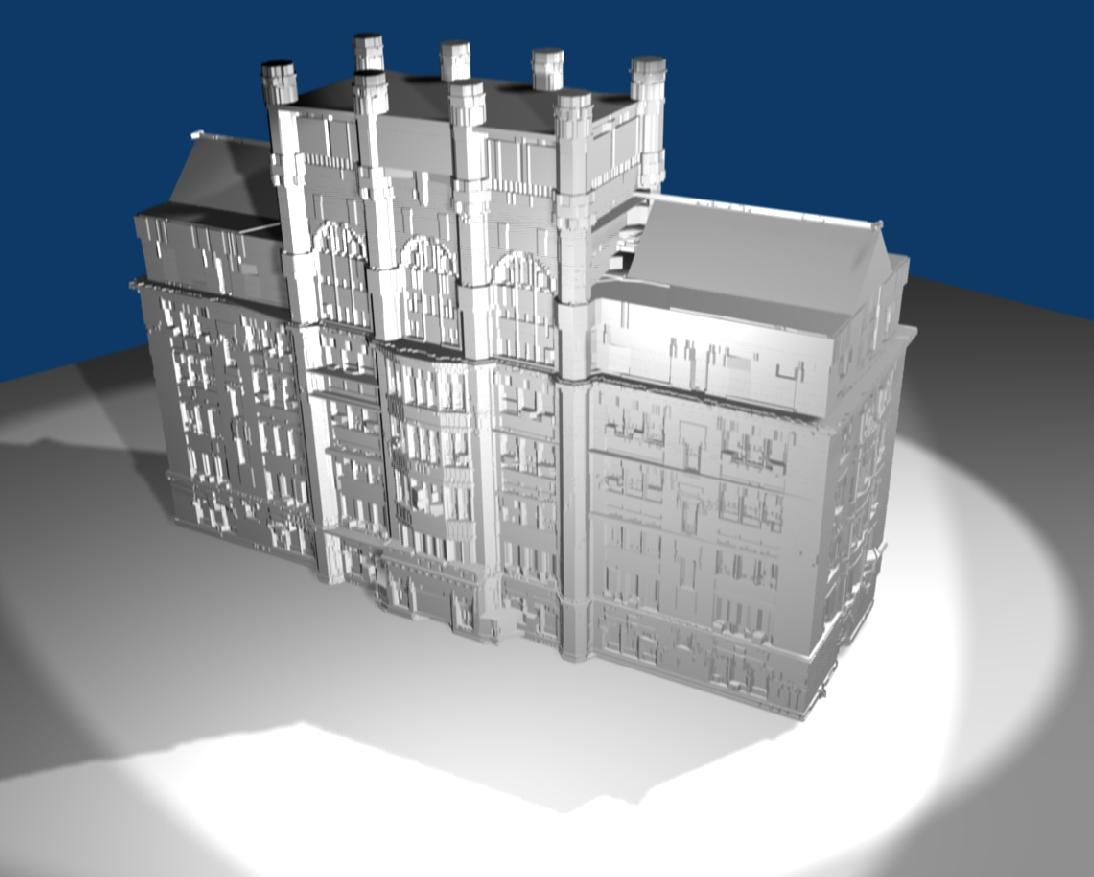
\includegraphics[width=0.8\textwidth]{HunterShaded.jpg} \\
(a) \\
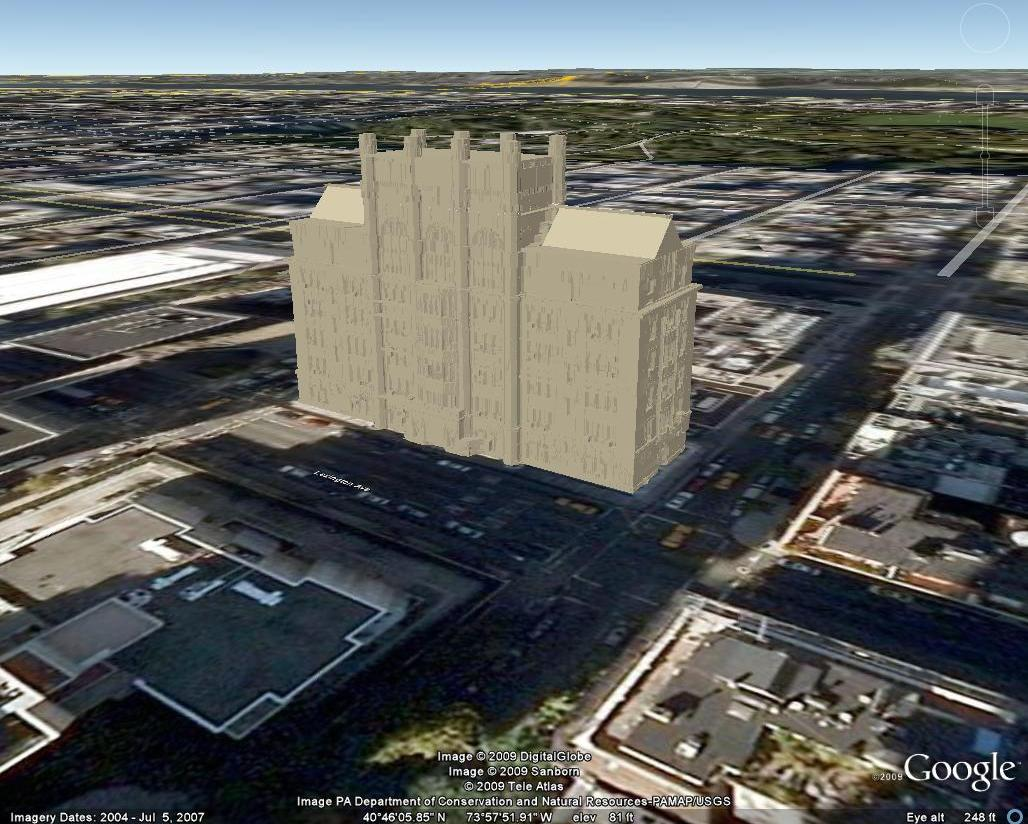
\includegraphics[width=0.8\textwidth]{HunterGE.jpg} \\
(b)
\end{tabular}
\end{center}
\caption{ (a) rendering of lightweight reconstructed model.
(b) The placement of the 3D model on Google Earth.}
\label{fig:OUT}
\end{figure*}

\begin{figure*}[htbp]
\begin{center}
\begin{tabular}{c}
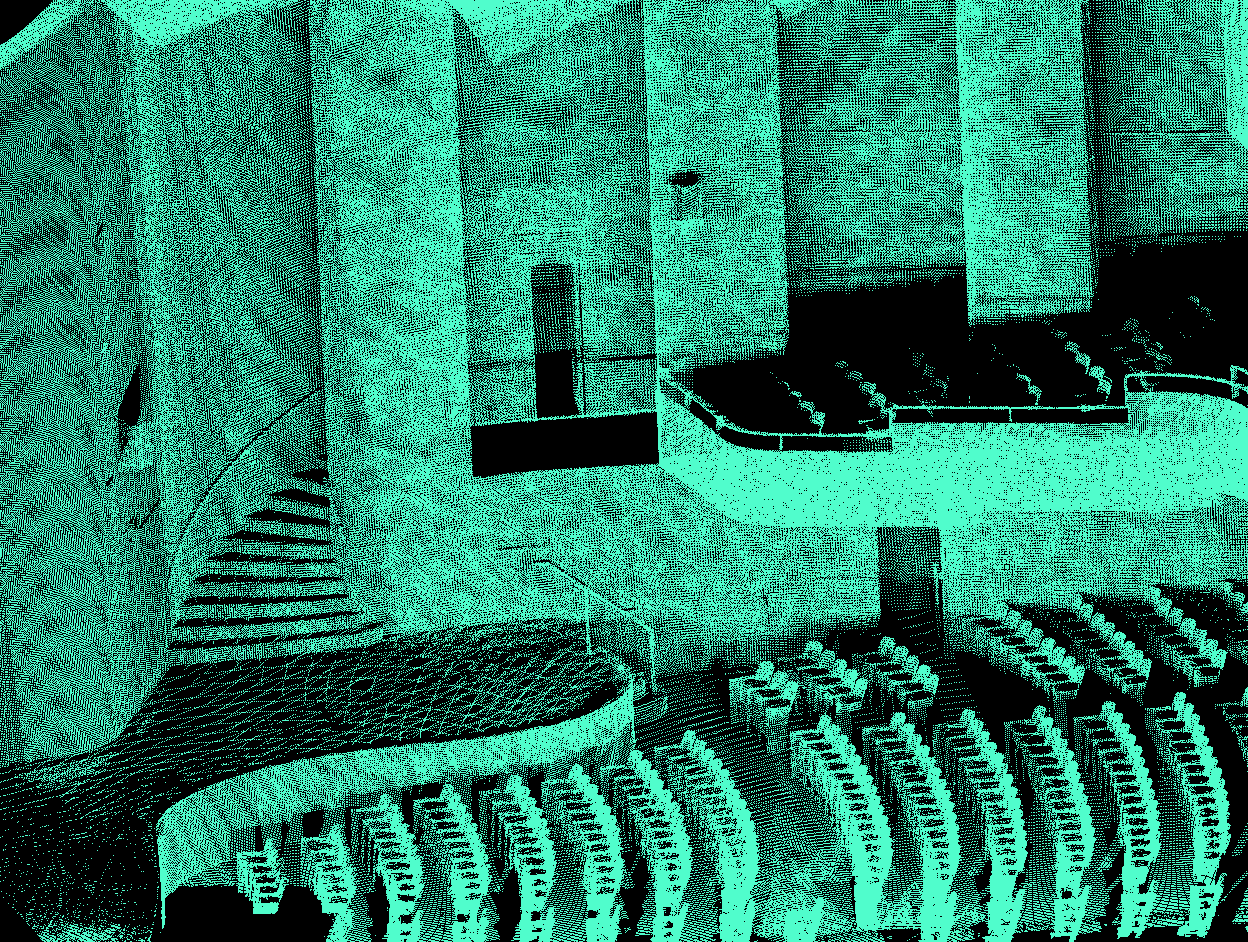
\includegraphics[width=0.8\textwidth]{range_crop.png} \\
(a) \\
\includegraphics[width=0.8\textwidth]{HunterTheatreShaded.jpg} \\
(b)
\end{tabular}
\end{center}
\caption{The model of an interior scan. (a) Point cloud data and the
(b) reconstructed lightweight 3D model.}
\label{fig:IN}
\end{figure*}

In addition to exterior models, we have also applied the lightweight
reconstruction algorithm to the range data of interior scans.
The snapshot of an interior scan is shown in \Figa{IN}
and its reconstructed 3D model is shown in \Figb{IN}.
This model is primarily reconstructed using the extrusion unit
upon the main structures of the interior.
The chairs and some other fine details were manually culled.
Please note that the model generated in \Figb{IN} is of low resolution.
Any lost detail may be recaptured by using a smaller threshold $\tau_d$
to obtain higher resolution models.

To measure the error of a reconstructed 3D model, we first transform it
to the 3D point cloud coordinate system.
The error $E$ is measured as the distance between the 3D points in the cloud
to their closest planes in the reconstructed model $M$:
\begin{equation}
E = \frac{1}{|X|}\sum_{x\in{X}}{d^2(x, M)}
\label{eq:em}
\end{equation}
where $X$ is the set of 3D points in the point cloud, and distance
$d(x, M) = \text{min}_{p \in M}\lVert x - p \lVert$ is the minimum
Euclidean distance from a 3D point $x$ to its closest face $p$ of $M$.

\begin{figure} [htbp]
\begin{center}
\begin{tabular}{c}
\includegraphics[width=0.8\textwidth]{error_1000_32_4.png} \\
(a) \\
\includegraphics[width=0.8\textwidth]{error_1000_4_1.png} \\
(b)
\end{tabular}
\end{center}
\caption{The deviation map of the 3D point cloud. (a) The result with $\tau_r$ = 4 and $\tau_d$ = 32.
(b) The result with $\tau_r$ = 1 and $\tau_d$ = 4. }
\label{fig:EM}
\end{figure}

To visualize the error between real 3D data and the inferred model,
we generate deviation map images.
Two such images are shown in \Fig{EM} for the point cloud data in
\Figb{IR_2_DXF}.
The deviation maps are constructed as follows.
For each face $p$ of $M$, a corresponding texture image is computed.
The intensity of each pixel in the texture image is determined by the error
of the corresponding 3D points computed by \Eq{em}.
The accuracy of the reconstructed model is controlled by Hausdorff distance
threshold $\tau_d$ and BPA refinement radius $\tau_r$.
Threshold $\tau_d$ determines the accuracy of keyslice detection and $\tau_r$
determines the accuracy of boundary vectorization.

\Tbl{em} lists the relationship among the $\tau_d$, errors,
number of faces, and model size for the input data in \Figb{IR_2_DXF}.
The units for $\tau_d$ and error is in pixels and millimeters, respectively.
The size of the original point cloud for the 3D building is more than 700 MB.
From the table, one can see that even for the most accurate model, the size
is dramatically reduced compared with the original 3D point cloud data.
This is a desirable property for web-based applications (\Figd{IR_2_DXF}).
The low resolution ($\tau_d = 64$) and high resolution ($\tau_d = 4$) models
were generated in 15 and 120 minutes, respectively,
on a laptop PC running an Intel Core 2 T7200 CPU at 2.0 GHz with 2.0 GB RAM.
Future work includes the optimization of the BPA vectorization module since
it consumes approximately 70\% of the computation time.

\setlength{\tabcolsep}{4pt}
\begin{table}[hbtp]
\begin{center}
\begin{tabular}[t]{||c||c|c|c|c||}
\hline
$\tau_{d} $(pixel) & Error (mm)& \# of faces & Size (KB) & time (s) \\ \hline \hline
64 & 0.658 & 1471  & 15  & 1977  (32'57'') \\ \hline 
32 & 0.294 & 3284  & 32  & 2353  (39'13'') \\ \hline
16 & 0.141 & 8574  & 86  & 3008  (50'08'') \\ \hline
8  & 0.131 & 13955 & 137 & 3696  (61'36'') \\ \hline
4  & 0.094 & 27214 & 261 & 5391  (89'51'') \\ \hline
2  & 0.088 & 31331 & 335 & 7586  (126'26'')\\ \hline
1  & 0.083 & 32187 & 337 & 10927 (182'07'')\\ \hline
\end{tabular}
\end{center}
\caption{Error measurements for reconstruction of Thomas Hunter dataset using
Hausdorff distance threshold $\tau_d$ and BPA radius threshold $\tau_r = 4$.}
\label{tbl:em}
\end{table}
\setlength{\tabcolsep}{1.4pt}


\setlength{\tabcolsep}{4pt}
\begin{table}[hbtp]
\begin{center}
\begin{tabular}[t]{||c||c|c|c|c||}
\hline
$\tau_{d} $(pixel) & Error (mm)& \# of faces & Size (KB) & time (s) \\ \hline \hline
64 & 0.085 & 5741   & 55  & 617  (10'17'') \\ \hline
32 & 0.063 & 8614   & 86  & 623  (10'23'') \\ \hline  % key slice 9'
16 & 0.052 & 9810   & 94  & 674  (11'14'') \\ \hline
8  & 0.028 & 15338  & 149 & 740  (12'20'') \\ \hline
4  & 0.022 & 42877  & 420 & 1042 (17'22'') \\ \hline
2  & 0.012 & 91736  & 988 & 1688 (28'08'') \\ \hline % key slice 9'
1  & 0.011 & 101466 & 990 & 1708 (28'28'') \\ \hline
\end{tabular}
\end{center}
\caption{Error measurements for reconstruction of Hunter Theater dataset using
Hausdorff distance threshold $\tau_d$ and BPA radius threshold $\tau_r = 4$.}
\label{tbl:em_theater}
\end{table}
\setlength{\tabcolsep}{1.4pt}

%%%%%%%%%%%%%%%%%%%%%%%%%%%%%%%%
%%%%%%   Model Comparison    %%%
%%%%%%%%%%%%%%%%%%%%%%%%%%%%%%%%
\section{Model Comparison}

Although models generated by 3D BPA are of high resolution, they usually
require excessive storage capacity.
The model in \Fig{TH_BPA}, for example, needs almost 400 MB of storage,
which prevents this solution from being applied to web-based applications.
One way to improve matters is to apply some approximation/decimation
technique to reduce the space required by these models.

The holes in the 3D BPA model in \Fig{TH_BPA} are present in the
original dataset.
They are due to the fact that the laser never reflected back to
the scanner after penetrating the glass windows.
The 3D BPA method is deficient in filling these holes.
We counter this problem by first applying a symmetry-based hole filling
algorithm on the 2D slices to create enhanced slices that are processed
by an adaptive 2D BPA method to fill gaps.
Finally, an extrusion operation is applied to create a watertight 3D model.

\begin{figure}[htbp]
\begin{center}
\includegraphics[width=0.8\textwidth]{BPA_TH.png}
\end{center}
\caption{Dense triangulated BPA mesh cropped from \Figb{IR_2_DXF}.}
\label{fig:TH_BPA}
\end{figure}

Among all mesh reduction techniques, {\it qslim} is one of the most
sophisticated and efficient algorithms.
We carried out a comparison between models generated by our proposed
method and those approximated by {\it qslim}.
The comparisons were conducted on models sharing the same number of faces.
It is worth noting that {\it qslim} ran out of memory on the 3D model data
generated by BPA in \Fig{TH_BPA}.
In order to reduce the size of the model for {\it qslim} to work, we had
to either down-sample the 3D model generated by BPA or split it into
sub-models which can be handled by {\it qslim}.

\begin{figure}[htbp]
\begin{center}
\begin{tabular}{cc}
\includegraphics[width=0.45\textwidth]{comp_32_2_qslim.png} &
\includegraphics[width=0.45\textwidth]{comp_4_2_qslim.png} \\
(a) & (b) \\
\includegraphics[width=0.45\textwidth]{comp_32_2.png} &
\includegraphics[width=0.45\textwidth]{comp_4_2.png} \\
(c) & (d)
\end{tabular}
\end{center}
\caption{
Models generated by {\it qslim} having (a) 2,000 and (b) 32,000 faces.
Models generated by our approach having (c) 2,000 and (d) 32,000 faces.}
\label{fig:TH_comp}
\end{figure}

\Figa{TH_comp} and \Figc{TH_comp} respectively depict the models generated
by {\it qslim} and our proposed method with approximately 2,000 faces each.
Higher resolution models with roughly 32,000 faces each are shown in
\Figb{TH_comp} and \Figd{TH_comp}.
Notice that the models approximated by {\it qslim} are inferior since they
do not preserve the sharpness of the original model and are replete with
holes. Our symmetry detector and extrusion operation guarantees no holes.

\newchapt{Future Work}{chapt9}{Future Work}


%%%%%%%%%%%%%%%%%%%%%%%%%%%%%%%%
%%%%%% Future Work           %%%
%%%%%%%%%%%%%%%%%%%%%%%%%%%%%%%%
\section{Conclusion and Future Work}

This paper has presented an efficient algorithm for lightweight 3D modeling
of urban buildings from range data.
Our work is based on the observation that buildings can be viewed as the
combination of two basic components: extrusion and tapering.
The range data is partitioned into volumetric slabs whose 3D points are
projected onto a series of uniform cross-sectional planes.
The points in those planes are vectorized using an adaptive BPA algorithm
to form a set of polygonal contour slices.
Prominent keyslices are extracted from this set.
Applying extrusion to these keyslices forms lightweight 3D models.
Experimental results on both exterior and interior urban building datasets
have been presented to validate the proposed approach.

We achieve further geometry compression by detecting a series of
slices that coincide with a taper operation.
In the current work, we demonstrate how to infer the taper-to-line
geometry structure.
In future work we will extend this to include the taper-to-point geometry
structure, which appears frequently in Gothic architecture (e.g., churches).
A nice characteristic of this structure is that the image slices will converge
to a point, which is a good inference cue.

Additional future work is to investigate the modeling of the ``follow-me''
geometry structure.
This is a more complicated geometry structure featured in Google SketchUp
that exists when the model can be reconstructed by moving a cross-sectional
unit along a curve trajectory.
We will track the slices to obtain the curve trajectory.
Finally, we will optimize the performance of the BPA vectorization module,
which consumes the bulk of the computation time.

\newchapt{The New Enhancement}{chapt10}{The New Enhancement}

%% \section{Major Plane Detection}
%% Given a point cloud dataset of a building, its major planes can be detected using plane based hough
%% transform method. Once the major planes are identified, we can rectify the dataset and project the
%% 3D data into 2D slices along the normals of those major planes.
%%
%% *. Major planeqs detection.
%%
%% *. Data Rectification.

\section{New Improvement Overview}

With the windows detection and segmentation improvement, the overview of the new enhancement is depicted 
in the \Fig{model_ov}. If there is no window or door detected at the window/door detection module, 
the window/door installation module would be skipped.

\begin{figure}[htbp]
  \centering
  \includegraphics
      [width=\textwidth]
      {model_overview.pdf}
      \caption{The flow diagram of the new enhancement.}
      \label{fig:model_ov}
\end{figure}


\section{Model Segmentation}

%% The main functionality of buildings is to provide a space for people to live or work.
%% Therefore, the main structure of them can be as simple as a box with windows.
%% On the other hand, buildings are the results of architectures, which can be considered as art.
%% This could make the structures of buildings extremely complicated.

Modeling a building as a whole structure from point cloud is complicated 
due to the natural complexity of buildings.
To tackle this issue, buildings should be split into simpler sub-structures for reconstruction.
We can utilize this divide and conquer strategy to segment the point cloud dataset of a building
and reconstruct each segmented dataset based on extrusion or tapered operations.
Once each segmentation is processed and modeled, they can be combined and merged into the whole final model.

%% (OPTION) We proposed a multi-resolution segmentation approach, that is separator based and keyslice based
%% segmentation. The idea is to first decompose the whole building using separator slices detected from
%% all major facades. This segmentation step is relative safe and precise in a sense that
%% the separators or salient planar feature generally separate parts from each other.
%% The segmentation consists of two steps; the first one is separate the data based on separators detected
%% in slices from all major directions. We shall obtain split data after the first step.
%% The second step is to further segment these split data if necessary.

As we know, different parts of a building are separated by walls, ledgers etc. 
These {\it ``separators''} provide clues for model segmentation. 
When projected onto 2D images, these separators have a common characteristic, 
that is a relative large {\it ``dark''} region representing a salient feature in black-white images.
For example, the roof and the body are divided by a ledger as shown in \Figc{MS_Fig1}.
\Figb{MS_Fig1} and \Figd{MS_Fig1} shows different parts of the roof are separated by walls.


\begin{figure}[htbp]
  \centering
  \includegraphics
      [width=\textwidth]
      {model_separate.pdf}
      \caption{The model segmentation: 
      (a) the original cooper union model.
      (b) the projected wall image from one face.
      (c) the projected wall image from another face.
      (d) the projected ledger image.}
      \label{fig:MS_Fig1}
\end{figure}

The model segmentation is carried out as follows:
First of all, for a given point cloud dataset, we'll compute separators from all major directions, 
including bottom-up and normals of facades. 
Because a building may have multiple facades with normals perpendicular to the bottom-up direction,
it is much easier to segment dataset in bottom-up direction if there is any separators detected.
The next step is to compute the segmentation image from the separators of those normals.
Finally, we segment the remaining dataset based on the segmentation image.

\subsection{Separator Detection}
\label{sec:sd}

We used a kernel based connected components (CC) method for separator detection. 
For each projected slice image $I_i$, the separator detector 
checks each data point $P_i$ using a 5x5 kernel $K$ centered at $P_i$.
Let $S_p$ be a set of points visited by the separator detector and $S_p$
is initialized to empty.
At the beginning, the point $P_i$ is checked against $S_p$ to 
determine whether it has been visited before. 
If not, $P_i$ is added into $S_p$ and the data points $N={P_j | P_j \neq P_i, P_j \in K}$ 
covered by $K$ are recorded.
If there are enough data points found in the neighbor, say $|N| > 12$, 
namely half of the kernel $K$, 
$P_i$ is considered as qualified point for a new connected component $C$.
For this case, $P_i$ is added to $C$. 
The same computation is applied to all new recorded data point in $N$, and 
qualified points are added into $C$. 
When there is no more new data point needs to be checked, the detector stops
and a new connected component, $C$, is detected.


The minimum and maximum coordinates, $x_{min}, x_{max}, y_{min}, y_{max}$, in $C$
are computed to obtain the rectangle boundary. 
To check whether $C$ represents a real separator, a testing is carried out:
\begin{equation*}
\left\{
\begin{array}{lr}
| x_{max} - x_{min} | > T_{size} \\
| y_{max} - y_{min} | > T_{size}
\end{array} \right.
\end{equation*}
where $T_{size}$ is a threshold representing the minimum size of the separator, 
usually a value of 16 is good enough to rule out all non-separators.
The above testing implies that a real separator CC should contains a big chunk of data
and its width and height should be at least $T_{size}$. 
If a connected component $C$ satisfies the above conditions, 
the slice index $i$ and the bounding information $x_{min}, x_{max}, y_{min}, y_{max}$, 
are logged down for further process.

\subsection{Dataset Segmentation}

The separators in all major directions computed in the previous section will be used for model segmentation.
If there are separators detected in bottom-up direction, the first step is to segment the dataset based on 
these separators. Because there is only one direction, the segmentation is straightforward.
The next step is to transform the separators in all other directions into the common coordinate.
As \Figa{DS_Fig1} shows, each separator is transformed into a line segment in the bottom-up 
projected image with the end points representing the bounding positions.
To divide the dataset, we need to know the exact boundary for each segmentation. 
This can be done by computing exact intersection point for each line segment with other line segments.


\begin{figure} [htbp]
\begin{center}
\begin{tabular}{cc}
\includegraphics[width=0.5\textwidth]{segment_roof_result.png} &
\includegraphics[width=0.5\textwidth]{segment_roof_regions.png} \\
(a) & (b) 
\end{tabular}
\end{center}
\caption{ Segmentation region computation:
      (a) the transformed image with line segment of the separators
      (b) the processed segment image}
\label{fig:DS_Fig1}
\end{figure}

Given a line segment $L_i = P_0P_1$, represented by two end points $P_0$, $P_1$, 
we can compute the intersection points of
$L_i$ with all other line segments. %[ with the equation of intersection computation of two planar lines].
If the result intersection point $P_i$ is falling outside of the image or 
is far away from either $P_0$ or $P_1$, $P_i$ can be skipped. 
When all the other line segments are checked, we can obtain two intersection points
, $P'_0$ and $P'_1$ which are the closest ones to $P_0$ or $P_1$ respectively. 
After intersection points are computed for all line segments, 
the segmentation image $I_s$ can be obtained as shown in \Figb{DS_Fig1}.

With the segmentation image $I_s$, the dataset segmentation is straightforward. 
We first build up a look-up table for each pixel in $I_s$ as shown in \Figb{DS_Fig1}. 
Different regions are marked in different colors and are assigned a unique region id $rid$. 
For any 3D point cloud data $P$, we can compute
its 2D projection location $(x, y)$ in the image $I_s$. %[ based on the equation [equation of the projection].
The region id for $P$ can be obtained from the look-up table based on $(x, y)$ coordinates.
In the example shown in \Figb{DS_Fig1}, 
totally 5 regions are identified and the original point dataset is split into 5 subsets for further process.

\section{Windows and Doors Detection}
\label{sec:wdd}

\begin{figure}[htbp]
  \centering
  \includegraphics
      [width=\textwidth]
      {model_win_comp.pdf}
      \caption{The thickness detection of the windows/doors:
      (a) the window on the original model
      (b) the projected slice viewing from bottom-up direction
      (c) the close-up view of the parallel lines and the distance $d_w$. }
      \label{fig:WD_Fig1}
\end{figure}

Windows and doors are important features for buildings to be modeled. 
%Furthermore, accurate computation of the extrusion structures requires these information.
%Without knowing the marked location as window part, 
%extra keyslices may be computed and hence lead to unnecessary extrusion operations. 
%[show a figure with unnecessary keyslice? how?]
The information we want to compute for windows and doors includes both the location and the thickness.
The thickness is computed based on the observation that two parallel lines can be detected
when viewing from the bottom-up direction as shown in \Figc{WD_Fig1} . 
For two parallel lines $L_1: y = mx + c_1$ and $L_2: y = mx + c_2$, 
% as shown in Fig1, http://www.askiitians.com/iit_jee-Straight_Line/Distance_between_two_parallel_lines
the distance $d_w$ is computed with the following equation,
\begin{equation*}
d_w = \frac{|c_1 - c_2|}{\sqrt{1 + m^2}}
\end{equation*}

%[Fig1: show the window thickness detection image, two parallel lines are drawn]
%[Fig2: show the projected windows/doors slice]

\begin{figure}[htbp]
  \centering
  \includegraphics
      [width=\textwidth]
      {window_result.pdf}
      \caption{The window information: (a)The projected windows slice
      (b) the most bottom-right window extracted from (a) with BPA contour in red. 
	(c) The contours of windows computed from (a).}
      \label{fig:WD_Fig2}
\end{figure}

Once the distance $d_w$ is computed, we can obtain the windows/doors image by projecting the data points
between $L_1$ and $L_2$ onto a slice image as shown in \Figa{WD_Fig2}. 
There are multiple window structures in the same projected slice image. 
We can use the same strategy as separator detection described in Section \ref{sec:sd}, that is,
kernel based connected component method, to isolate each window for processing. 
\Figb{WD_Fig2} shows a window extracted as a connected component and BPA algorithm was applied
to obtain the contour in red.
After walking through the image shown in \Figa{WD_Fig2} for all the connected components 
and applying BPA on them, 
the final results show all the detected window contours as depicted in \Figc{WD_Fig2}.
These contours will be used to add windows and doors onto the final model.

%% \subsection{Windows and Doors Mask Image Generation}
%% 
%% After computing the windows and doors structures for each facade, 
%% these information can be used for accurate keyslice detection. 
%% As we mentioned before, the keyslice detection based on Hausdorff distance criteria may
%% introduce unnecessary keyslice due to the data of windows or doors. 
%% To tackle this issue, we can construct a series of windows and doors mask images 
%% from the computed structures and therefore eliminate those unnecessary keyslices.
%% 
%% With the information computed on the windows, the mask image generation is straightforward.
%% For each window, we can obtain the 3D bounding box around it based on the $d_w$ and
%% the size of the window in 2D image. The task is to convert these 3D bounding box for each
%% window to corresponding rectangle in 2D slices for each direction. 
%% Once we get this rectangle box for a direction, say $X$, we can use it as a mask when
%% computing keyslices in $X$ direction.
%% 
%% [Figaxxx] shows that 4 projected window slices and the rectangle boxes in bottom-up direction
%% for all windows in all 4 directions are shown in [Figbxxx]. 
%% Likewise, we can generate similar mask image for other directions.
%% 


\section{Model Reconstruction}

When underline structures of all segmentations have been computed, we can start to reconstruct the whole model.
The reconstruction of a single segmentation is straightforward: transform the underline geometry polygon to
3D coordinate system; for an extrusion structure, it is a push-pull operation of the basic geometry;
for a tapered structure, it is a face constructions between the base line segment and the corresponding
converging point.

The reconstruction becomes more complicated when multiple segmentations need to be merged since
some segmentations may share the same vertices or edges. Therefore model merging needs to be done
for the reconstruction of the whole model.

\subsection{Model Merging}


\begin{figure}[htbp]
  \centering
  \includegraphics
      [width=\textwidth]
      {model_merge.pdf}
      \caption{Vertices adjustment for model merging
      (a) the two new points $Q_0$ and $Q_1$ are projected to an existed line as $Q'_0$ and $Q'_1$.
      (b) after (a), $Q'_1$ is merged with an existed point $P_1$.
      (c) after (a), both $Q'_0$ and $Q'_1$ are merged with existed point $P_0$ and $P_1$ respectively.
      (d) one of the point $Q_1$ is too far away for adjustment. }
      \label{fig:MR_Fig1}
\end{figure}

The first segmented part can be easily reconstructed without merging. 
Let ${\bf M}$ represent all lines or planes added into the final model so far. 
When adding a new line segment $Q_0Q_1$ to the model, 
we need to compute the closest line ${\bf L} = P_0P_1$ in ${\bf M}$ to $Q_0Q_1$.
Let $d = max(dist(Q_0, {\bf L}), dist(Q_1, {\bf L}))$, i.e., the larger distance 
between $Q_0$ to ${\bf L}$ and $Q_1$ to ${\bf L}$.
The distance from a point $Q$ to a line ${\bf L}$ can be computed using the equation:
\begin{equation*} % point to line equation
d(Q, { \bf L}) = | {\bf w - (w \cdot u) \, u} |
\end{equation*}
where ${\bf w} = (Q - P_0) $ and {\bf u} is the unit direction vector of {\bf L}.

There are several cases to be considered.
If $d <= \delta$, that is, both $Q_0$ and $Q_1$ are close enough to $L$, the projected point $Q'_0$ and $Q'_1$
are used to replace $Q_0$ and $Q_1$ respectively as shown in \Figa{MR_Fig1}. 
Furthermore, if one of the projected point, say $Q'_1$ is close to an end point of $L$, say $P_1$, 
$Q'_1$ would be merged with $P_1$ as shown in \Figb{MR_Fig1}. 
If both $Q'_0$ and $Q'_1$ are matched with $P_0$ and $P_1$, 
the line $Q_0Q_1$ would be merged totally with the line $L$, which was shown in \Figc{MR_Fig1}.
However, if $d > \delta$, no merging should be conducted as shown in \Figd{MR_Fig1}. 
\Figa{MR_Fig2} and \Figb{MR_Fig2} show the structures before and after model merge.


\begin{figure} [htbp]
\begin{center}
\begin{tabular}{cc}
\includegraphics[width=0.45\textwidth]{model_before_merge.png} &
\includegraphics[width=0.45\textwidth]{model_after_merge.png} \\
(a) & (b) 
\end{tabular}
\end{center}
\caption{ 
      (a) two structures inside red ellipse are separated before merge
      (b) new structures after merge}
\label{fig:MR_Fig2}
\end{figure}

\section{Windows and Doors Installation}

After the model merging, the whole reconstructed model has been generated. 
We call this {\it naked} model in that there is no windows or doors yet as shown in \Figa{WDR_Fig1}.
If the point cloud contains windows or doors, we need to add them onto the naked model.
The window and door structures have been computed as described in Section \ref{sec:wdd},
now we need to know on which face or plane should they be added.

\begin{figure} [htbp]
\begin{center}
\begin{tabular}{cc}
\includegraphics[width=0.45\textwidth]{model_naked.png} &
\includegraphics[width=0.45\textwidth]{model_windows.png} \\
(a) & (b) 
\end{tabular}
\end{center}
\caption{ Windows and doors reconstruction:
      (a) the reconstructed naked model.
      (b) the whole model with windows and doors added.}
\label{fig:WDR_Fig1}
\end{figure}

Let {\bf M} be the set of lines from a naked model.
Let $Q_0 = [X_{min}, Y_{min}], Q_1 = [X_{max}, Y_{max}]$ define the bounding box of a window $w$,
i.e., $[Q_0, Q_1]$ is the diagonal points for $w$.
Let $[Z_{min}, Z_{max}]$ be the height range of $w$.
The goal is to find the right face (closest line segment) for $w$ to be added.
For each line segment $L = P_0P_1 $ in ${\bf M}$, we first compute the projected points $Q'_0, Q'_1$
of $Q_0, Q_1$ on $L$ to check whether they are in between $[P_0, P_1]$. 
If not, $L$ is not eligible for adding $w$ since a window could not fall outside of a facade. 
Otherwise, the extruded range $L_{min}, L_{max}$ of $L$ is computed.
If $Z_{min} > L_{min}$ and $Z_{max} < L_{max}$, that is, the window $w$ is totally covered by the 
extruded face $F$ which is generated from $L$, $F$ is a potential face for adding $w$.
The distance $d_p = max(|Q_0Q'_0|, |Q_1Q'_1|)$ is used
to compare with global minimum distance $d_{p\_min}$ which was set to be a large value initially.
If $d_p < d_{p\_min}$, which means a closer face for $w$ is found, $d_{p\min}$ is updated to $d_p$ and
the corresponding line $L_{win}$ and its face $F_{win}$ are updated to $L$ and $F$ respectively. 

When all lines in ${\bf M}$ are checked, $F_{win}$ will give us the right face for adding $w$.
To add $w$ on $F_{win}$, we need to compute the projected point $P'$ for each vertex $P$ in $w$ on $F_{win}$.
Let $F_{win} = ax + by + cz + d$, the equation to compute $P(x_0, y_0, z_0)$ is
\begin{equation*} % projection point on a plane
P' = P - \frac{(ax_0+by_0+cz_0+d)}{a^2+b^2+c^2}\,{\bf n}
\end{equation*}
where {\bf n} is the normal of $F_{win}$.
This will generate a closed face $F_w$ on $F_{win}$. 
A simple push-pull operation on $F_w$ with the distance $d_w$ which was computed in the Section \ref{sec:wdd} 
will add the window $w$ onto $F_w$ of the naked model.
\Figb{WDR_Fig1} shows the entire model with windows and doors added for the model in \Figa{WDR_Fig1}.


\section{Experimental Results}

We have applied the proposed method on some synthetic datasets. The synthetic dataset were generated
from Sketchup models which were downloaded from Sketchup 3D warehouse. Essentially, the synthetic
dataset generator samples 3D point cloud data based on the face information extracted from the
Sketchup models. A parameter is used to control the sample rate of the face.

\Fig{ER_Fig1} through \Fig{ER_Fig10} shows the experimental results. For each set of the figures,
the original Sketchup model is shown in (a), the snapshot of the synthetic dataset sampled from (a)
is shown in (b). (c) and (d) shows the snapshots of the reconstructed model from different viewpoints.

However, there are some limitations on the proposed method. First of all, the error introduced in
early stages could be propagated to later stages, which could largely affect the final results.
For example, if the computation of the major faces introduces some errors and therefore the detected
the normals of the faces are not precise enough, the generation of the projected slices would be
problematic and the keyslices computation may be failed, which leads to the failure of the extrusion
structure detection.

Another limitation of the proposed method is that it could not handle the intersection of two
structures from different directions. For example, \Figa{ER_Lmt} shows a case where two extruded
structures intersect and \Figb{ER_Lmt} shows a case with intersection of a tapered structure and
an extruded structure. Both of them could not be handled by the proposed approach yet.

\begin{figure} [htbp]
\begin{center}
\begin{tabular}{cc}
\includegraphics[width=0.5\textwidth]{cu_1.png} &
\includegraphics[width=0.5\textwidth]{cu_2.png} \\
(a) & (b) \\
\includegraphics[width=0.5\textwidth]{cu_3.png} &
\includegraphics[width=0.5\textwidth]{cu_4.png} \\
(c) & (d)
\end{tabular}
\end{center}
\caption{Experimental Results of Cooper Union model:
      (a) original Sketchup model.
      (b) synthetic point cloud data generated from (a).
      (c) reconstructed model (I) .
      (d) reconstructed model (II).}
\label{fig:ER_Fig1}
\end{figure}

\begin{figure} [htbp]
\begin{center}
\begin{tabular}{cc}
\includegraphics[width=0.5\textwidth]{spitak_1.png} &
\includegraphics[width=0.5\textwidth]{spitak_2.png} \\
(a) & (b) \\
\includegraphics[width=0.5\textwidth]{spitak_3.png} &
\includegraphics[width=0.5\textwidth]{spitak_4.png} \\
(c) & (d)
\end{tabular}
\end{center}
\caption{Experimental Results of Spitak model:
      (a) original Sketchup model.
      (b) synthetic point cloud data generated from (a).
      (c) reconstructed model (I) .
      (d) reconstructed model (II).}
\label{fig:ER_Fig2}
\end{figure}

\begin{figure} [htbp]
\begin{center}
\begin{tabular}{cc}
\includegraphics[width=0.5\textwidth]{house_1.png} &
\includegraphics[width=0.5\textwidth]{house_2.png} \\
(a) & (b) \\
\includegraphics[width=0.5\textwidth]{house_3.png} &
\includegraphics[width=0.5\textwidth]{house_4.png} \\
(c) & (d)
\end{tabular}
\end{center}
\caption{Experimental Results of house model:
      (a) original Sketchup model.
      (b) synthetic point cloud data generated from (a).
      (c) reconstructed model (I) .
      (d) reconstructed model (II).}
\label{fig:ER_Fig3}
\end{figure}

\begin{figure} [htbp]
\begin{center}
\begin{tabular}{cc}
\includegraphics[width=0.5\textwidth]{branch_lib_1.png} &
\includegraphics[width=0.5\textwidth]{branch_lib_2.png} \\
(a) & (b) \\
\includegraphics[width=0.5\textwidth]{branch_lib_3.png} &
\includegraphics[width=0.5\textwidth]{branch_lib_4.png} \\
(c) & (d)
\end{tabular}
\end{center}
\caption{Experimental Results of Branch library model:
      (a) original Sketchup model.
      (b) synthetic point cloud data generated from (a).
      (c) reconstructed model (I) .
      (d) reconstructed model (II).}
\label{fig:ER_Fig4}
\end{figure}

\begin{figure} [htbp]
\begin{center}
\begin{tabular}{cc}
\includegraphics[width=0.5\textwidth]{clements_lib_1.png} &
\includegraphics[width=0.5\textwidth]{clements_lib_2.png} \\
(a) & (b) \\
\includegraphics[width=0.5\textwidth]{clements_lib_3.png} &
\includegraphics[width=0.5\textwidth]{clements_lib_4.png} \\
(c) & (d)
\end{tabular}
\end{center}
\caption{Experimental Results of Clements library model:
      (a) original Sketchup model.
      (b) synthetic point cloud data generated from (a).
      (c) reconstructed model (I) .
      (d) reconstructed model (II).}
\label{fig:ER_Fig5}
\end{figure}

\begin{figure} [htbp]
\begin{center}
\begin{tabular}{cc}
\includegraphics[width=0.5\textwidth]{doe_1.png} &
\includegraphics[width=0.5\textwidth]{doe_2.png} \\
(a) & (b) \\
\includegraphics[width=0.5\textwidth]{doe_3.png} &
\includegraphics[width=0.5\textwidth]{doe_4.png} \\
(c) & (d)
\end{tabular}
\end{center}
\caption{Experimental Results of Doe library model:
      (a) original Sketchup model.
      (b) synthetic point cloud data generated from (a).
      (c) reconstructed model (I) .
      (d) reconstructed model (II).}
\label{fig:ER_Fig6}
\end{figure}

\begin{figure} [htbp]
\begin{center}
\begin{tabular}{cc}
\includegraphics[width=0.5\textwidth]{health_town_1.png} &
\includegraphics[width=0.5\textwidth]{health_town_2.png} \\
(a) & (b) \\
\includegraphics[width=0.5\textwidth]{health_town_3.png} &
\includegraphics[width=0.5\textwidth]{health_town_4.png} \\
(c) & (d)
\end{tabular}
\end{center}
\caption{Experimental Results of Health Town library model:
      (a) original Sketchup model.
      (b) synthetic point cloud data generated from (a).
      (c) reconstructed model (I) .
      (d) reconstructed model (II).}
\label{fig:ER_Fig7}
\end{figure}

\begin{figure} [htbp]
\begin{center}
\begin{tabular}{cc}
\includegraphics[width=0.5\textwidth]{miami_1.png} &
\includegraphics[width=0.5\textwidth]{miami_2.png} \\
(a) & (b) \\
\includegraphics[width=0.5\textwidth]{miami_3.png} &
\includegraphics[width=0.5\textwidth]{miami_4.png} \\
(c) & (d)
\end{tabular}
\end{center}
\caption{Experimental Results of Miami Date Court model:
      (a) original Sketchup model.
      (b) synthetic point cloud data generated from (a).
      (c) reconstructed model (I) .
      (d) reconstructed model (II).}
\label{fig:ER_Fig8}
\end{figure}

\begin{figure} [htbp]
\begin{center}
\begin{tabular}{cc}
\includegraphics[width=0.5\textwidth]{simple_1.png} &
\includegraphics[width=0.5\textwidth]{simple_2.png} \\
(a) & (b) \\
\includegraphics[width=0.5\textwidth]{simple_3.png} &
\includegraphics[width=0.5\textwidth]{simple_4.png} \\
(c) & (d)
\end{tabular}
\end{center}
\caption{Experimental Results of simple model:
      (a) original Sketchup model.
      (b) synthetic point cloud data generated from (a).
      (c) reconstructed model (I) .
      (d) reconstructed model (II).}
\label{fig:ER_Fig9}
\end{figure}

\begin{figure} [htbp]
\begin{center}
\begin{tabular}{cc}
\includegraphics[width=0.5\textwidth]{michael_1.png} &
\includegraphics[width=0.5\textwidth]{michael_2.png} \\
(a) & (b) \\
\includegraphics[width=0.5\textwidth]{michael_3.png} &
\includegraphics[width=0.5\textwidth]{michael_4.png} \\
(c) & (d)
\end{tabular}
\end{center}
\caption{Experimental Results of St Michael church model:
      (a) original Sketchup model.
      (b) synthetic point cloud data generated from (a).
      (c) reconstructed model (I) .
      (d) reconstructed model (II).}
\label{fig:ER_Fig10}
\end{figure}

\begin{figure} [htbp]
\begin{center}
\begin{tabular}{cc}
\includegraphics[width=0.5\textwidth]{limitation_1.png} &
\includegraphics[width=0.5\textwidth]{limitation_2.png}
\end{tabular}
\end{center}
\caption{Examples of failed cases:
      (a) intersection of two extruded structures.
      (b) intersection of a taper structure with an extruded structure.}
\label{fig:ER_Lmt}
\end{figure}

%% We need to consider keyslice detection and segmentation.
%%
%% 0. major direction/normal detection. (Hadi's planar HT)
%%
%% 1. exam keyslices from all possible directions, including bottom-up, normals of facades.
%%
%% 2. pick up a direction based on the number of keyslices:
%%
%%   2.1. If there is only one keyslice found in a particular direction, stop.
%%   2.2. If a separator (big trunk data) is detected, mark this slice for segmentation.
%%   2.3. If high frequency keyslices starting from a keyslice $k_i$, mark $k_i$.
%%   2.4. For bottom up direction, segment the data based on 2.2 and 2.3.
%%   2.5. For facade direction, where normals(unit) fall into the same plane, construct an image with inputs of all marked pages.
%%
%% 3. for each segmented point cloud $R_i$, go back to 1.
%%
%% 4. only consider separator as segmentation mark, ignore the extrusion with taper without separator.
%%
%% LIMITATION:
%% *. Could not handle sub-component with extrusion coupled with tapered structure where the separation direction is not
%%    the same as the tapered direction.
%% *. Could not handle intersection of two extrusions from different directions.



% LocalWords:  chapt keyslice fixpoint lr DS keyslices mx WD BPA vertices htbp
% LocalWords:  WDR Sketchup Lmt Spitak pdf CC CCs png downloaded

%   \newchapt{Introduction}{chapt1}{Introduction}

The 3D modeling of urban buildings is an area of active research
with increasing attention drawn from the computer graphics and
computer vision communities.
Current state-of-the-art algorithms include procedural modeling,
3D laser scanning, and image-based approaches.
In addition, conventional modeling tools are commonly used for this purpose.
The most accurate input source for modeling {\it existing} buildings, though,
remains laser range scanners.
They provide high geometric detail by collecting range data from hundreds
of meters away with an accuracy on the order of a few millimeters.
This fidelity is appropriate for construction, architecture, cultural
heritage, and forensics applications.
Unfortunately, laser range scanning can produce an overwhelming amount of data,
which poses great challenges to visualization software that require lightweight
3D models for interactive use.
Polygonal data generated from range scans are therefore too dense for use in
web-based applications such as Google Earth and Microsoft Virtual Earth.
These applications work best with lightweight models consisting of only
hundreds of polygons.

The goal of this work is to automatically produce high-quality
lightweight models of urban buildings from large-scale 3D range data.
The proposed solution is inspired by the simple paradigm embedded in
procedural modeling as well as interactive tools such as Google SketchUp.
The core of these methods is that a simple set of extrusion and taper
operations applied to 2D contours can grow a wide array of complex 3D urban
models.
We propose a reverse engineering approach to infer key cross-sectional
planar contours along with a set of extrusion and taper operations to derive
lightweight models that conform to the 3D range data.

The proposed algorithm can generate models across a wide spectrum of
resolutions.
A particularly useful feature of the algorithm is that it outperforms
existing approximation techniques by preserving the sharpness of the raw
data, even at low resolution.
The contribution of this work is that it combines the benefits of
\emph{a priori} knowledge of urban buildings and fast 2D image
processing techniques to perform 3D modeling of urban buildings directly
from point cloud data.
This offers the benefit of a cost-effective geometry compression
approach for voluminous range data within the domain of urban structures.
It can be applied to boost web-based 3D applications, virtual city touring,
and online gaming.

\section{Related Work}

In an attempt to steer clear of tedious and expensive hand-made models,
procedural modeling of buildings in \cite{PMB_MWH,PMB_WWS,PMB_PM} has been proposed.
By using an effective description language, buildings and streets of a virtual
city can be generated automatically.
The strength of this approach is that the description language can generate
a huge number of buildings and streets quickly and beautifully.
This is particularly useful for gaming and other computer graphics applications.
However, since the parameters used to generate the buildings are randomly
generated, the city generated with these buildings and streets is a virtual one.
This approach is not useful for attempting to model an {\it existing} building.
In order to do so, one has to manually specify the parameters of the building,
which is very cumbersome.
Our goal is to automatically infer the contours and extrusion/taper parameters
of an existing building directly from dense range data.

Reconstruction of 3D models from range data has been addressed in
\cite{RE_Fisher,RE_CLF,RE_CD} with applications in numerous research areas,
including computer-aided design (CAD), computer vision, architectural modeling,
and medical image processing.
In \cite{DP_OWYC}, the authors proposed a 3D building reconstruction from a
2D floorplan image.
With the help of a 2D floorplan image, both the interior and exterior of a
building can be reconstructed accordingly.
A survey on methods for generating 3D building models from architectural
floor plans is given in \cite{YIN09}.
However, reliance on 2D floor plans makes this approach too limiting for
most applications, including our project.
In \cite{RE_TOGSH}, known manufacturing features were used to infer the
3D structure of mechanical parts.
Their method benefits from the domain knowledge that most of the mechanical
parts consist of predefined structures, such as holes, bosses, and grooves.
Our work is partially motivated by this idea since it also incorporates
{\it a priori} knowledge about the construction of urban buildings for further
inference.
However, their method is based on predefined simple geometry structures and
the assumption that the input 3D data has no holes.
This hinders their approach for those applications with incomplete data.

Medical image processing techniques are usually dealing with low SNR data.
There has been a lot of work on the medical 3D image reconstruction as in
\cite{MIR_FJS, MIR_BMMNB, MIR_KL, MIR_SKJ, MIR_SMHC, MIR_BVC}.
The basic ideas behind these approaches
are 3D reconstruction from sliced or histologic images using interpolation techniques.
The statistical inference are also intensively used to infer the low SNR images. For example,
In \cite{MIR_FJS}, Sigworth tried to deal with low SNR image data using maximum-likehood approach.
Because most of the statistical processes are computational intensity,
these approaches usually are heavy-duty approaches in order to obtain accurate, high resolution models.

Multimodal data fusion is another approach for large-scale urban
environment modeling.
In \cite{UM_Zakhor,UM_HYN}, both air and ground data are fused, including
laser scans, camera images, and aerial images.
The LIDAR scans are used to create the models and the camera images are used
for texture mapping.
Citing the cumbersome and expensive use of laser scanners, the researchers
in \cite{AKBARZADEH06} propose an approach that relies solely on passive
sensors (cameras) mounted on a moving vehicle.
Dense 3D point cloud measurements are derived using their multiview stereo
module based on multiple plane sweeping directions.
In an attempt to compress the voluminous data produced in the method of
\cite{AKBARZADEH06}, Xiao et al. \cite{UM_XFTQ} introduced an alternate
approach for modeling facades along a street using prior knowledge about
the buildings.
They achieve geometry compression and deliver a clean approximation of the
facades by applying a combination of plane fitting and window detection.
Their method, however, relies on limited assumptions about the planarity of
the buildings.
The method introduced in this paper, however, places no such limitations.
We can handle facades of any shape that exploit extrusion and taper operations.

The ball-pivoting algorithm (BPA) \cite{BPA_BMRS} is an efficient technique
for meshing 3D point clouds to produce polygonal models.
The generated meshes, however, constitute heavyweight models,
with the number of vertices nearly approaching the number of points in the
3D point cloud.
This limits its usefulness for web-based applications.
Although a BPA model can be simplified using approximation techniques such as
{\it qslim} \cite{BPA_GH}, the sharp detail of the original model is not
preserved.

In addition to the aforementioned research projects carried on in academia, 
some commercial products are developed in start-up companies. 
In \cite{IND_YC}, the buildings in Manhanttan are modeled to enhance
the virtual reality of social network. The buildings are accurately modeled via
aerial LIDAR data and were associated with address and related social information.
The most related commercial product is EdgeWise\textsuperscript{\texttrademark}, 
a new developed product by ClearEdge\textsuperscript{3D} \cite{IND_EW}.
In EdgeWise integrated development environment (IDE), the 3D point data 
(in pts or ptz format) can be loaded and visualized. And then, as an initial step,
ground extraction is applied to classify the point cloud data. 
Essentially, the point cloud in the same planar are marked. 
The next step is to infer the polygons from the scan data based on the classification. 
Once the polygons are inferred, the model is
exported to CAD format (dxf) and can be edited in Google SchetchUp. 
As a matter of fact, the CAD model it produced contains a lot of noisy and spikes. 
Basically, this commercial tool provides a good starting point for editing. 
It can only handle planar at this point in time and 
the resolution of the model it generated is not adjustable.


%%%%%%%%%%%%%%%%%%%%%%%%%%%%%%%%
%%%%%%   Overview  %%%%%%%%
%%%%%%%%%%%%%%%%%%%%%%%%%%%%%%%%
\section{Overview}

We propose an efficient way to reconstruct 3D models from range data by
partitioning the data into thin cross-sectional volumetric slabs.
For each slab, all range data in that slab is projected onto a 2D
cross-sectional contour slice.
Producing this array of slices permits us to avoid costly computation directly
on 3D data.
A similarity measure \cite{IR_Brown, IR_ZF, RE_WWLZ} is used to 
cluster the sliced images together into {\it keyslices}.
This term is analogous to the use of ``keyframes'' in computer animation,
which denotes important snapshots in the animation sequence from which
intermediate results can be derived.
In essence, each keyframe is a slice in the spatiotemporal volume of
an animation.
Similarly, each keyslice is a 2D image which contains a {\it transitional}
cross-section of the building, encapsulating major contours in the facade.
The model is then generated by applying basic extrusion and taper
operations from one keyslice to the next.
This produces a lightweight representation consisting of only a few
hundred polygons.

\begin{figure}[htb]
  \centering
  \includegraphics[width=\textwidth]{flow.pdf}
      \caption{Flow graph for proposed approach}
      \label{fig:flow}
\end{figure}

An overview of our approach, depicted in \Fig{ov}, begins with the
acquisition of a dense 3D point cloud $C$ of a building.
$C$ is then partitioned into a nonoverlapping set of volumetric slabs.
Each slab $S$ is associated with one projection plane $P$,
sitting at the base of $S$.
The purpose of partitioning $C$ is to establish a set of cross-sections,
or contour slices.
By examining the changes among these slices, we can identify the prominent
slices, or {\it keyslices}, as well as the necessary extrusion and
taper operations that must apply to them to generate the model.
By casting this 3D modeling task into a series of 2D operations, we
reduce the dimension of the problem to achieve a significant savings in
computational complexity.

To generate the 3D model of a building, all these key raster images need 
to be vectorized to represent the silhouette or boundary of the building. 
Couple of raster image vectorization approaches are
proposed in \cite{DP_AAKMT, DP_DP, DP_WM}. The Douglas-Peucker
algorithm tried to connect all the existed points to form a polygon. 
Although the implementation of
this approach is very efficient with the improvement in \cite{DP_HS},  this method cannot
handle the case where some extra interior points are existed as some outlier data.
To tackle this issue, Medeiros et al. \cite{BPA_MVL} applied ball-pivot algorithm (BPA)
\cite{BPA_BMRS}, which was original proposed on 3D point cloud data, on the 2D image to obtain
vectorized boundary. The key parameter for BPA to work successfully is to find the right size of
the ball for pivoting. We have proposed an adaptive BPA algorithm to solve this problem.

\begin{figure}[htbp]
\begin{center}
\includegraphics[width=1.0\textwidth]{overview.pdf}
\end{center}
\caption{Overview of the proposed approach.}
\label{fig:ov}
\end{figure}

Due to occlusion and material-dependent reflection problems off of glass
(e.g., windows), the input data is incomplete and noisy.
Therefore, noise removal and hole filling are carried out as a
preprocessing stage to generate the 3D model.
The next stage of the approach is to carry out fast image processing
techniques on the enhanced image slices to detect keyslices.
Boundary vectorization for these raster keyslices is then conducted to
transform these points into polygons.
Tapered structure detection is carried out to further reduce the model size.
Finally, 3D model generation is achieved by applying the extrusion/taper
operations to the keyslices to reconstruct lightweight 3D models of urban
buildings from range data.

\newchapt{Preprocessing on Range Data}{chapt2}{Preprocessing on Range Data}

%%%%%%%%%%%%%%%%%%%%%%%%%%%%%%%%
%%%%%%   PREPROCESSING  %%%%%%%%
%%%%%%%%%%%%%%%%%%%%%%%%%%%%%%%%
%\section{Preprocessing the Range Data}
\label{sec:prep}

The input to our system is range data assembled as a 3D point cloud.
Our data is obtained from a Leica Cyrax 2500 laser range scanner \cite{RDP_LRS},
which works by sweeping an eye-safe laser beam across the scene to collect
up to one million 3D depth points per frame.
All scene points that lie within 100 meters can be acquired with an accuracy
of 5mm in depth.
The basic algorithm that we use for registering the voluminous 3D data
acquired from multiple scans of buildings has been introduced in
\cite{RDP_LS}.
That same algorithm is also responsible for extracting the major axes
of the building in order to align it to the axes of the world coordinate
system.
This is necessary to properly infer the keyslices.
\Figb{IR_2_DXF} displays a properly aligned, {\it registered} 3D point cloud
consisting of 14 scans totalling 14 million points.

\begin{figure}[htbp]
\begin{center}
\begin{tabular}{c}
	\includegraphics[width=0.6\textwidth]{HunterPhoto.jpg} \\
	(a)\\
	\includegraphics[width=0.6\textwidth]{point_cloud.png} \\
	(b)
\end{tabular}
\end{center}
\caption{
(a) Image of building to be modeled.
(b) 3D point cloud of building assembled by registering multiple scans.
}
\label{fig:IR_2_DXF}
\end{figure}

Due to occlusions and limited vantage points, the point cloud collected by the
laser scanner contains artifacts and holes.
In addition, computing directly on 3D data is time-consuming and
computationally complex.
To tackle these issues, we define inner and outer bounding boxes for the
building to clip away unrelated scene objects.
Then, we convert the 3D modeling problem into a set of 2D problems by
projecting the 3D data into a series of 2D cross-sectional contour images.
Noise removal, hole filling, and vectorization are all done in this
2D space.

%%%%%%%%%%%%%%%%%%%%%%%%%%%%%%%%
%%%%%% 3D Data Rectification %%%
%%%%%%%%%%%%%%%%%%%%%%%%%%%%%%%%
\section{Point Cloud Rectification}
\label{sec:rect}

%% Put the flow of the data rectification.
Although the multiple scans of point cloud data have been registered, 
they are not rectified as depicted in \Fig{pc_orig}. 
Please note the point cloud has been sub-sampling by a factor of 50.
This is not suitable for our further 3D modeling.
As one of the pre-processing steps, this registered data will be rotated
and translated to be aligned with world coordinates.

%% Put the image of rectfied data.
\begin{figure}[htbp]
\begin{center}
\begin{tabular}{c}
\includegraphics[width=\textwidth]{BPA_TH.png}
\end{tabular}
\end{center}
\caption{ The registered point cloud without rectification. }
\label{fig:pc_orig}
\end{figure}

As we know, there are a lot of line features existed in the point cloud, which
provides a good clue for rectifing the data. 
For each scan $s$ of the scene, we can obtain a set of line segments $L_s$. 
Assume $T_s$ is the transformation matrix for the scan $s$ to be registered with other scans.
In other words, for any point $P(x,y,z)$ in the scan $s$, $P*T_s$ will transform the
point $P$ into the final registered coordinate system as shown in \Fig{pc_orig}.

We can obtain the major axises by clustering these line segemetns $L_s$ from different
scans. The purpose of clustering is to group the lines whose direction are very close to each other.
To cluster these lines, we first transform the line segments in $L_s$ into world
corrdinate system using $T_s$ as described above. After transformation, we will
get a larger line set $L = {l_1, l_2, \ldots, l_n}$. For each line $l_i$, we first
normalize it to a unit vector:
\begin{equation*}
\bar{l_i} = \frac{l_i}{\parallel l_i \parallel}
\end{equation*}

The unit vector $\bar{l_i}$ has the unique length 1, which provides a good starting point 
for clustering since we do not need to worry the length of the lines. 
An array of bins are used to hold the unit vectors.
As the initial step, the first line $\bar{l}$ is picked up and is insert into the 
first bin and set the counter of the bin to 1.
When a new unit vector $\bar{l_n}$ is observed, we try to see whether there is an
existed unit vector in the bins which has similar direction as $\bar{l_n}$. This is
done by computing the distance $d_{\pm}=\parallel \pm\bar{l_n} - \bar{l_i} \parallel$.
Because $\bar{l_n}$ can has two opposite directions, we can compute both of them and
choose the smaller value as the distance $d$. If $d$ is smaller enough, $\bar{l_n}$
is clusterd with the line $\bar{l_i}$ and the counter of the bin holding $\bar{l_i}$
is increased by 1. On the other hand, if $d$ is big, we have to compare $\bar{l_n}$
with a line in the next bin. If $\bar{l_n}$ could not fit any line in the bins, we
will insert $\bar{l_n}$ into a new bin and set the counter of the bin to 1. 
To avoid the bias of the initial select, each unit vector $\bar{l_i}$ is
adjusted to be the mean of all unit vectors falling inside this bin. 

Once we go through all the lines in $L$, the clustering is complete. 
The next step is to choose the major axises from the clustering results. 
Essentially, this is to choose bins whose counters are among largest. 
Assume $u$, $v$, and $n$ represent the three largest bins. This is demonstrated in
\Fig{pc_orig} in red, green and blue respectively. To rectify the data,
we can refer to the following transformation matrix $\mathbf{M}$:
\begin{figure}[htbp]
\begin{center}
\begin{tabular}{c}
\includegraphics[width=0.5\textwidth]{point_cloud_rect_matrix.png}
\end{tabular}
\end{center}
\caption{ The transformation matrix. }
\label{fig:pc_rect_matrix}
\end{figure}

\begin{equation*}
\mathbf{M} = \left(
\begin{array}{cccc}
u_x & u_y & u_z & -e_x \\
v_x & v_y & v_z & -e_y \\
n_x & n_y & n_z & -e_z \\
  0 &   0 &   0 &    1 
\end{array} \right)
\end{equation*}

This is illustrated in \Fig{pc_rect_matrix}. $(x, y, z)$ is the world coordinate system.
The rectified coordinate system is represented using $(u, v, n)$. 
The vector $[-e_x, -e_y, -e_z]^T$ is the translation of the view point from the world origin.
After the transformation with $\mathbf{M}$, the new data set and the three major line segments are
shown in \Fig{pc_rect}.

%% rectified data
\begin{figure}[htbp]
\begin{center}
\begin{tabular}{c}
\includegraphics[width=\textwidth]{BPA_TH.png}
\end{tabular}
\end{center}
\caption{ The rectified point cloud of \Fig{pc_orig}. }
\label{fig:pc_rect}
\end{figure}


\section{Extraction of 2D Slices}
\label{sec:image_slicing}

We consider the point cloud data as a large array of 3D points to be
sliced into horizontal volumetric slabs.
All 3D points within each slab are projected onto a horizontal projection
plane, or slice, at the base of the slab.
\Fig{slice_slab} shows the 3D point cloud in \Figb{IR_2_DXF} partitioned into
50 slabs.
The 3D points in each slab are projected onto a projection plane to
form cross-sectional contour slices.
\Fig{slicing} depicts four such slices, associated with the four displayed
projection planes of \Fig{slice_slab}.

\begin{figure} [htbp]
\begin{center}
\begin{tabular}{c}
\includegraphics[width=0.6\textwidth]{slab_noplanar.png} \\
(a) \\
\includegraphics[width=0.6\textwidth]{slab_planar.png} \\
(b)
\end{tabular}
\end{center}
\caption{
(a) Slabs of the 3D point cloud data are used to determine prominent
cross-sections upon which extrusion/taper operations are applied.
(b)The 3D point cloud of \Figb{IR_2_DXF} partitioned into uniform
volumetric slabs.
The 3D points in each slab are projected onto a projection plane to
form cross-sectional slices. Four such planes are shown.}
\label{fig:slice_slab}
\end{figure}

The height of each slab is $\boldsymbol{\delta}$.
If $\boldsymbol{\delta}$ is held constant, each slice is generated from
equi-spaced slab intervals.
If $\boldsymbol{\delta}$ is allowed to vary, then we may
choose to allow for large values in parts of the structure that are similar,
and low values in regions that contain finer detail.
To avoid working on 3D data directly, a relatively small constant value
for $\boldsymbol{\delta}$ is chosen to generate 2D cross-sectional image slices.

\begin{figure} [htbp]
\begin{center}
\begin{tabular}{cc}
\fbox{\includegraphics[width=0.45\textwidth]{image_slice_0190.png}} &
\fbox{\includegraphics[width=0.45\textwidth]{image_slice_0600.png}} \\
(a) & (b) \\
\fbox{\includegraphics[width=0.45\textwidth]{image_slice_0714.png}} &
\fbox{\includegraphics[width=0.45\textwidth]{image_slice_0951.png}} \\
(c) & (d)
\end{tabular}
\end{center}
\caption{The set of slices corresponding to the four projection planes in
\Fig{slice_slab}.}
\label{fig:slicing}
\end{figure}

Without loss of generality, the $y-$axis is used to represent the bottom-up
vertical direction.
Over each slab in height range $[H_{lo}, H_{hi})$,
we project the 3D data $\boldsymbol{P}(x,y,z)$, for $H_{lo} \leq y < H_{hi}$,
onto a 2D image slice.
The projection is normalized in the range $[0,W]$, where $W$ is the image width:
\begin{equation}
[\,x^{2D},\; y^{2D}\,]^T = \omega\cdot[\,x^{3D}_i - X_{MIN},\; z^{3D}_i - Z_{MIN}\,]^T
\label{eq:image_slicing}
\end{equation}
Note that $\omega = W/(X_{MAX} - X_{MIN})$, and that
the [$X_{MIN}$, $X_{MAX}$] and [$Z_{MIN}$, $Z_{MAX}$] pairs define the
3D bounding box, which can be obtained through user input and can be used
to clip away noise data.
\Fig{slicing}(a)-(d) show some examples of the 2D slices, where noise
and incomplete data are observed.


%   \newchapt{Slice Enhancement}{chapt3}{Slice Enhancement}

%%%%%%%%%%%%%%%%%%%%%%%%%%%%%%%%
%%%%%%   Slice Enhancement  %%%%
%%%%%%%%%%%%%%%%%%%%%%%%%%%%%%%%
\section{Hole Filling}
\label{sec:mdr}

The slices we extract above often have holes (i.e., missing data) due to
occlusion or other visibility issues.
Fortunately, most urban buildings have symmetry that we can exploit to
fill these holes.
Symmetry computation on 3D data is an active research topic, such as those in
\cite{Sym_PSGRF,Sym_ZPA,Sym_TW,Sym_MGP}, which has potentially numerous applications.
However, symmetry computation 3D data directly is expensive. 
Here, we only conduct this computation on the 2D image slices.
Since the 3D data has been already rectified \cite{RDP_LSYGS} and projected onto 2D slices, hence only 2D translation
is needed to be considered for symmetry computation.
Let $P(x,y)$ be a point on the original image $I$ and $P'(x',y')$ be the reflected
point of $P$ with respect to a symmetry line $L$.
The symmetry computation equation for $L$ is as follows:
\begin{equation}
L = \underset{x,y}{\operatorname{arg\,min}}\sum{d_{x,y}(P', I)}
\end{equation}
where the $d_{x,y}(P',I)$ is the distance between the self-reflected point
$P'$ and its nearest data point in image $I$.
The reflected point $P'$ of the original point $P$ is computed with
respect to a line along either the $x-$ or $y-$ axis.
Therefore, the symmetry line $L$ is obtained as the line with minimum
summation error over the reflected data points.
\Figa{sym} and \Figb{sym} depict the original input with holes, and
the output after hole filling using symmetry computation, respectively.

\begin{figure}[htbp]
\begin{center}
\begin{tabular}{c}
\fbox{\includegraphics[width=0.6\textwidth]{image_slice_0705_0711.png}} \\
(a) \\
\fbox{\includegraphics[width=0.6\textwidth]{image_slice_0705_0711_recoverd.png}} \\
(b)
\end{tabular}
\end{center}
\caption{ Symmetry-based hole filling. (a) Original 2D slice image and
(b) output image after hole filling.}
\label{fig:sym}
\end{figure}


%   \newchapt{Keyslice Detection}{chapt4}{Keyslice Detection}

%%%%%%%%%%%%%%%%%%%%%%%%%%%%%%%%
%%%%%%   3D Reconstruction  %%%%
%%%%%%%%%%%%%%%%%%%%%%%%%%%%%%%%
%\section{Lightweight 3D Reconstruction}
\label{sec:reconst}
Our 3D modeling algorithm is based on \emph{a priori} knowledge that
urban buildings can be created through a series of extrusion and taper
operations on the salient cross-sections contained in the keyslices.
\Fig{keyslices} depicts the keyslices derived from the uniform slices
given in \Fig{slice_slab}. 
The key step for successful modeling is identifying these salient cross
sections upon which the extrusion and taper operations will apply.

An intuitive way for key slice detection is to compute the similarity between the sliced images.
In other words, the sliced images are clustered into different groups based on the similarity among them.
There are two mainly research methods for similarity measurement of 2D images: area based method and feature based
methods. The area based methods are computational efficient but they usually can only be applied on
binary or gray-scale images. The feature based one is computational complex but more powerful and can be applied
to images obtained using different sensors, such as multi-modal image registration.
% read similarity measure papers.
Because our goal is to develop light-weight efficient algorithm for model reconstruction, plus
the input for similarity measure is pure binary images, the area based method is adopted for our approach.

The classical measure for area based method is the normalized cross
correlation \cite{DIP_Pratt}:
\begin{equation*}
CC(i,j) = \frac{\sum_W(W - E(W))(I_{(i,j)}-E(I_{(i,j)}))}
{\sqrt{\sum_W(W - E(W))^2}\sqrt{\sum_{I_{(i,j)}}(I_{(i,j)} - E(I_{(i,j)}))^2}}
\end{equation*}
where $W$ is an image mask, $E(W)$ is the mean of the mask's pixels, and $E(I_{(i,j)})$
is the mean of the image pixels covered by the mask $W$.
However, this method is very time consuming and is a local window-based approach,
which could not capture the global relations between images. Therefore, we proposed a
light-weighted global and efficient key image detection approach based on Hausdorff distance 
and curvatures computation.

\begin{figure}[hbtp]
\centering
\includegraphics[width=0.8\textwidth]{figures/keyslice_wireframe.png}
\caption{Keyslices derived from the input in \Fig{slice_slab}.}
\label{fig:keyslices}
\end{figure}

\section{Hausdorff Distance Based}
\label{sec:ksd}
The 2D image slices of an extruded region are similar to each other.
Thus, to detect the keyslices that delimit extruded regions one only needs
to compute the similarity between adjacent slices.
We select the Hausdorff distance \cite{IR_HKR} as the similarity measure.
Let $P_r(x_r, y_r)$ be a data point in a reference image and
let $P_i(x_i, y_i)$ be a data point in a new observed image $I$.
The Hausdorff distance of image $I$ to reference image $I_r$ is defined as:

\begin{equation}
d_H(I, I_r) = \sum_{i=0}^Nd_{min}(P_i, I_r)
\label{eq:hd}
\end{equation}

where $d_{min}(P_i, I_r)$ is the minimum distance from data point $P_i$
in image $I$ to the reference image $I_r$.
Alternatively, we can also define the Hausdorff distance, $d_H(I_r, I)$,
from reference image $I_r$ to a new observed image $I$, using \Eq{hd}.
These two distances are usually not equal to each other.
As a rule of thumb, one can choose
$d_{HD} = \text{MAX}\{d_H(I, I_r), d_H(I_r, I)\}$ as the Hausdorff distance.
To compute the keyslices, a threshold $\tau_{d}$ is used for the
Hausdorff distance $d_{HD}$.
If $d_{HD} < \tau_{d}$, the two images $I$ and $I_r$ are considered
similar to each other.
Otherwise, a keyslice image is found and $I_r$ is updated with $I$,
the new keyslice image.

\section{Curvature Based}
The accuracy of the keyslices detected by using the Hausdorff distance
is closely tied to threshold $\tau_d$.
Small $\tau_d$ leads to more accurate models and will require more time and
space to compute and store the result.
When the threshold $\tau_d$ is relatively large, potential keyslices which
contain salient structure may be missed.
Therefore, there is a trade-off between model accuracy and time-space
efficiency.
To address this problem, the curvature information is computed as a
complementary criteria for keyslice detection.

This idea is based on the observation that the keyslices are generally
located at large curvature changes along 2D slices extracted in the orthogonal
direction (e.g., side view), as shown in \Figa{HT_BPA_Curvature}.
Therefore, instead of computing the difference between two images directly,
we compute the curvature of orthogonal 2D slices, map the positions of
curvature extrema back to cross-sections in the original set of volumetric
slabs, and mark these cross-sections as keyslices.

\begin{figure}[htbp]
\begin{center}
\begin{tabular}{cc}
\fbox{\includegraphics[width=0.3\textwidth]{image_slice_lr_0580_0590_half.jpg}}
\fbox{\includegraphics[width=0.3\textwidth]{image_slice_lr_0830_0842_half.jpg}} &
\fbox{\includegraphics[width=0.3\textwidth]{curvature_center_lines_old_half.jpg}} \\
(a) & (b)
\end{tabular}
\end{center}
\caption{Curvature-based key slice detection.
(a) A partial set of two 2D sliced images from the orthogonal direction (side
view). The complete set will be used to extract the keyslices shown in
\Fig{keyslices}.
(b) The average curvatures detected over all of the sliced images along the
orthogonal direction.}
\label{fig:HT_BPA_Curvature}
\end{figure}

In the close-up view of a small region as shown in \Fig{KSD_Curv},
two curvatures, $c_1$ and $c_2$, are
computed in this small region. The red, blue and green lines indicate the locations
of the center, the starting and the ending of a curvature. 
As a matter of fact, there is a third curvature computed around the
black box sitting on top of the green line of the curvature $c_1$. 
However, this third one should not be consider as a real curvature 
in that the black box is due to an air conditioner during the data acquisition process, 
which means it is not a part of the building. We called this third curvature
{\it outlier curvature} which needs to be removed from the set of real curvatures.
Based on the fact that these outlier curvatures exist only in a few 2D slices,
we can exclude them by counting the number of appearance for each curvature.
Only those curvatures appears in most of the 2D slices are kept for further computation.

Once the real curvatures are obtained, they can be used as a complemental way of 
Hausdorff distance for keyslices detection. 
Each curvature $c$ is mapped to a set $s$ of original 2D cross-sectional
slices, $i,\ldots,j$, where $i$ and $j$ are corresponding to the starting and 
the ending locations of $c$. After this, the set $s$ is checked whether 
it contains any keyslice or not.
If a keyslice $k$ has been marked in $s$ by Hausdorff distance, 
nothing needs to be done and this curvature $c$ is discarded. 
On the other hand, if $s$ contains no keyslice, $i$ and $j$ will be marked as 
two new keyslices to keep the salient feature identified by this curvature $c$.
The combination of Hausdorff distance measurement and curvature inference
ensures that the salient structures of a building will be preserved.

%%% Figure of the tapered template.
\begin{figure}[htbp]
\begin{center}
\begin{tabular}{c}
\includegraphics[width=0.60\textwidth]{curvature.png}
\end{tabular}
\end{center}
\caption{ Curvature based key slice detection. }
\label{fig:KSD_Curv}
\end{figure}
%%% End of Figure

To compute the curvature, we first apply the slice extraction algorithm
described in \Sec{image_slicing} to obtain a series of 2D cross-sectional
images in the orthogonal direction.
We then apply the ball-pivot algorithm described in \Sec{BPA} to
vectorize the boundary for each sliced image.
We locate those curvatures that appear in most of the sliced images as the
places where keyslices are found, as shown in \Figb{HT_BPA_Curvature}.
Note that the red lines indicate location of the center of the curvature,
and the blue and green lines indicate the entering and exiting of the
curvature structures, respectively.
The combination of Hausdorff distance measurement and curvature inference
ensures that the salient structures of a building will be preserved.

\section{Loal Matching Based on Segmentation}

The keyslice detection described above are based on global information matching.
The strength of these methods lies on the effective of computation and they can
also produce good results on exterior scanning as depicted in \Fig{keyslices}. 
However, when applied to interior scannings when the layout of the structures 
is complex, there may be some limitations on these methods. 
As depicted in \Fig{ksd_gbl_bad}, the pillars inside the hall can be reconstructed
by simple extrusion of the base polygon. However, they are divided to 
excessive amount of keyslices because the dissimilarity of the outside window
structures in the same projection level. In other words, due to global matching
strategy, some independent objects which could be modeled using simple extrusion
operation are modeling using excessive keyslices. Although the reconstructed
models are still correct at this situation, they are not efficiency. That is, much
more keyslices are created to represent the simpled extruded parts. 

A more effective way for modeling the above structures is to model the different 
structures individually. By doing this, we can simply model the pillars using a
extrusion operation based on a base polygon. Certainly, for the complicate window
structures, more keyslices are still required but these keyslices would not contain
any pillar structures. To do this, segmentation is a necessary step to identify
all different parts of the scannings. 

There are a lot of literatures on image segmentation as in \cite{segmentation}. 
% a little bit survey on image segmentation, especially binary image segmentation.
% why the graph-cut is well-fit for our purpose.

Our segmentation based keyslice detection approach is an iterative algorithm.
We first applied the graph cut
on the 2D sliced binary image. The initial input to graph cut is done as follows. 
First of all, a random data point $p$ was located in the binary image $I$. The data
point $p$ is then growing to form an region $r$ based on the connected components 
until it reaches a fix-point. That is, no more data point can be reached in $r$. $r$
is taken as input by graph cut algorithm to compute the segmentations. 
The segmented objects (non-background pixels) are then stored and their pixels are 
reset to background pixels for next iteration. The algorithm is depicted in \Fig{alg_seg}.
To adjust the accuracy of the graph cut, the parameter ??? was used. To get more
accurate segments, which means more objects may be classified, enlarge/shrink its value.

For each new 2D image slice, there is a set of segmented objects $s$ is computed
by the above graph cut approach. Therefore, the keyslice detection problem is converted
into similarity measurement of the detected segments along the specified direction, 
e.g., vertical direction.
The similarity measurement is now among the segmented regions instead of the whole
contour of a sliced image. A global data structure, $T$, which contains all the current 
active segmented objects is maintained for matching. $T$ is initialized with the
detected segments from the first 2D slice which is regared as reference slice. 

For each new observed 2D slice, we first compute a set of segmented objects $s$. 
After this, we are trying to search for a matched segmented object $o'$ in $s$ for 
each existed active segmented objects $o$ in $T$. This searching process again is 
based on the Hausdorff distance described in \ref{ksd}. If such a matched object $o'$
exists, $o$ will be kept in $T$ as an active segmented object for next round of
computation. Otherwise, $o$ is removed from $T$ and is treated as a completed part or
object in the range data. At the same time, for any object $o'$ in $s$, if it is 
not found to be a matched segments for active objects in $T$, $o'$ will be added
to $T$ as a starting slice of a new part in range data and will be taken into
account for next adjance 2D slice computation. We keep doing this until the last
2D slice is visited and processed. Once the last slice is reached, all the active
segments in $T$ will be considered as the ending point of the objects in the range data.

The result obtained by the aboved local based keyslice detection is illustrated in 
\Fig{ksd_lcl_good}. As we can see, the pillar structures of the hall are reconstructed
using the simple extrusion operations, which is much more efficienct in terms of 
model size and representation.








%   \newchapt{Boundary Vectorization}{chapt5}{Boundary Vectorization}

After the keyslices are detected, $N_K$ keyslices will be identified
from a total of $N_A$ image slices.
Depending on the threshold $\tau_{d}$, $N_K$ is usually about one to two
orders of magnitude smaller than $N_A$, e.g., $N_K/N_A$ is 0.06 when
$\tau_d$ = 4.0 for the example in \Figb{IR_2_DXF}.
To generate the 3D model, these keyslice images need to be vectorized to
represent the contours of the building facade.
The difficulty of the problem lies in outliers and holes of non-perfect images.
We proposed a general framework based on an adaptive 2D ball-pivot algorithm (BPA) 
 to efficiently suppress the noisy, fill holes and generate contours for those images.

\section{Ball Pivot Algorithm (BPA)}
\label{sec:BPA}

STARTING POINT SELECTION
\\
\\
GAP DETECTION
\\
\\
RIGHT ANGLE RESHAPE
\\
\\


There exists numerous works on boundary vectorization,
such as those described in \cite{DP_RP,DP_LC,DP_AAKMT}.
However, these approaches
only consider the cases where perfect raster image data is provided.
For non-perfect data, these proposed methods were failed in various cases.
The problem considered here is to compute contours
for non-perfect binary images which may contain holes
along the boundary as well as noise or outliers
inside the boundary. Here, {\it boundary} refers to the
out-most region of any raster image and
{\it contour} refers to a vectorized boundary.


The Douglas-Peucker (DP) algorithm \cite{DP_DP} is widely used
to compute boundary vectorization for binary images.
Although  with the improvement of implementation described in \cite{DP_HS, DP_HS94},
the complexity of this approach is of $O(nlogn)$, this method cannot fill the
holes of the noisy data or handle the case
where spurious interior points are presented.
Agarwal et al. \cite{DP_AV} considered the problem of
approximating a polygon chain using another one to minimize the number of
vertices. However, for a raster image, the vertices
defining the contour were not known.
For example, \Figa{failed_case} shows a binary cross-section
image of a 3D point cloud data of a building. \Figb{failed_case} shows
the contour generated from DP algorithm. The problem is that there are
a lot of holes along the contour and the noise data inside of the
boundary are modeled inappropriately.
To tackle these issues, a general boundary vectorization framework is proposed
based on ball-pivoting algorithm (BPA) \cite{BPA_BMRS} which was used
originally on 3D point cloud data process to generate 3D mesh representation.
\Figc{failed_case} shows
the contour computed by the proposed framework which fills holes between gaps
and suppresses noise inside the boundary.


\begin{figure*}[hbtp]
\begin{center}
\begin{tabular}{c}
\includegraphics[width=0.8\textwidth]{BPA_init.pdf} \\
(a) \\
\includegraphics[width=0.8\textwidth]{BPA_refine.pdf} \\
(b)
\end{tabular}
\end{center}
\caption{Adaptive ball pivoting algorithm:
(a) Initial pivoting with a ball of radius 2$r$;
(b) Refinement with a ball of radius $r$.}
\label{fig:BPA}
\end{figure*}


The idea of the BPA is straight-forward:
pivot a ball on a starting point in the image
until it touches another data point as depicted in \Figa{BPA}.
Add the new touched
data point into an ordered list as the vertices of the contour polygon and
set it as the new pivoting point.
Keep doing this pivoting process until all data points are touched.

\section{Boundary Vectorization}
The basic idea behind the proposed framework for contour computation is as follows:
apply BPA on a selected starting point until
either the ball pivots back to the starting point which indicates a closed boundary is detected,
or the ball reaches a gap which means this contour is a non-closed
contour and one of the end points is reached.
Because the ball can start pivoting along either clock-wise direction or counter clock-wise direction,
another pivoting process at start pivoting from the other direction is conducted.
When both directions have been explored, a contour computation is done.
After this, the refinement process is carried out for each line segments using the same BPA algorithm.
For this refinement, the starting point is now the first end point of a line
and the stopping case is that the ball reaches the other point or it
reaches a gap.

Here is more detailed description for the algorithm.
At the initial BPA stage, a relatively large radius $r$ is chosen as a coarse step to cover all gaps between data points.
The output of the initial BPA, $\boldsymbol{\Phi}$, contains an ordered list of the boundary data
points $\boldsymbol{P}$ and their corresponding directions $\overrightarrow{\boldsymbol{R}}$ in which
the ball $C$ starts pivoting.
The BPA refinement process applies a smaller radius, say $r' = r/2$,
to $\boldsymbol{\Phi}$ to get more accurate results, as shown in \Figb{BPA}.
For this stage, the length of each line segment formed by adjacent points is checked,
$\ell = \overline{P_0P_1}$, in $\boldsymbol{\Phi}$.
For long line segments, the BPA is applied between the two adjacent points.
When the ball reaches the second end point, a new list of ordered boundary points,
$\boldsymbol{\Phi'}$, is inserted into $\boldsymbol{\Phi}$ between $P_0$ and
$P_1$.
This process continues until it finishes checking every adjacent point in $\boldsymbol{\Phi}$.
The refinement stops when $r'$ falls below threshold $\tau_r$.

The key parameter for the BPA algorithm to work successfully is finding
a good initial size of the ball for pivoting.
Here are some general guidances for choosing the radius. If a contour is known to be a closed polygon,
the initial radius should be big, e.g. the width of an image, to cover all gaps along the boundary.
Otherwise, if a boundary consists of sub-boundaries, one could select a relative small radius to start.

An example on the proposed framework is shown in \Fig{BPA_refinement}.
The initial BPA takes radius $\tau_r$ = 128,
which produced a coarse contour as shown in \Figa{BPA_refinement}.
\Figb{BPA_refinement} - \Figd{BPA_refinement} show that the contour is becoming more
accurate as the radius $\tau_r$ decreases from 32 to 2. Note that the original
image size is 1024x392 pixels as shown in \Figa{failed_case}.

\begin{figure}[htbp]
\begin{center}
\begin{tabular}{cc}
\fbox{\includegraphics[width=0.45\textwidth]{BPA_TH.png}} &
\fbox{\includegraphics[width=0.45\textwidth]{BPA_TH.png}} \\
(a) & (b) \\
\fbox{\includegraphics[width=0.45\textwidth]{BPA_TH.png}} &
\fbox{\includegraphics[width=0.45\textwidth]{BPA_TH.png}} \\
(c) & (d)
\end{tabular}
\end{center}
\caption{Boundary vectorization of a binary image with (a) radius = 128
(b) radius = 32 (c) radius = 8 (d) radius = 2.}
\label{fig:BPA_refinement}
\end{figure}


\begin{figure*}[htbp]
\begin{center}
\begin{tabular}{c}
\fbox{\includegraphics[width=0.7\textwidth]{BPA_TH.png}} \\
(a) \\
\fbox{\includegraphics[width=0.7\textwidth]{BPA_TH.png}} \\
(b) \\
\fbox{\includegraphics[width=0.7\textwidth]{BPA_TH.png}} \\
(c) 
\end{tabular}
\end{center}
\caption{(a) An example of binary image.
(b) The vectorization result based on DP algorithm and
(c) The vectorization result from proposed BPA algorithm.}
\label{fig:failed_case}
\end{figure*}

\begin{figure*}[htbp]
\begin{center}
\begin{tabular}{c}
\fbox{\includegraphics[width=0.7\textwidth]{aaa_image_slice_0529.png}} \\
(a) \\
\fbox{\includegraphics[width=0.7\textwidth]{bbb_image_slice_1024_392_0533_refine_with_rad_1_and_merged.png}} \\
(b) \\
\fbox{\includegraphics[width=0.7\textwidth]{bbb_image_slice_1024_392_0533_combine_HT_BPA_rad_32.png}} \\
(c)
\end{tabular}
\end{center}
\caption{Boundary vectorization of noisy binary image.
(a) the binary image to be processed.
(b) the contour computed by proposed method.
(c) the contour obtained by simplification with Hough transform.}
\label{fig:HT_BPA_figure}
\end{figure*}

\section{Contour Simplification}
\label{sec:BPA_HT}
%%% Adaptive BPA + HT %%%%

Although the proposed framework is an efficient and straightforward approach to
vectorize the contours of noisy images,
it might produce many short line segments for some special boundaries. An example
is shown in the upper part of the contour in \Figb{HT_BPA_figure} (Please see this
in zoomed-in mode). Here, each colored segment represents a contour edge.
One way to reduce the number of vertices of the polygon is to apply
the approximation polygon method in \cite{DP_AV}. The drawback of this
method is that the topological structures, such as straight lines, would be lost.
To solve this issue, a Hough transform (HT) based method is proposed to replace
short line segments with long lines and potentially eliminate noisy
or outlier vertices around the boundary.

To combine the adaptive BPA with HT, one can first apply the HT algorithm on the
original raster image $I$ to obtain all straight lines $\boldsymbol{L}$ and sort them by length.
The longer lines give higher confidence to the line structure of the underly images.
Then a dilation operation with 8-connected neighbors on $I$ can be used to get the dilation image, $I_d$.
The next step is to measure how well the lines in $\boldsymbol{L}$ match with
data in $I_d$, which determines whether a line in $\boldsymbol{L}$
should be used as a substitution or not.

If a line segment $L$ is found to be a good candidate, the next step is to
find the corresponding part of the BPA points in $\boldsymbol{\Phi}$ for
substitution. The first step is to compute the closest two points
$P_i$ and $P_j$ in $\boldsymbol{\Phi}$ to the two end points of $L$.
If the vertices in $\boldsymbol{\Phi}$ represent a polygon, they will have
a circle layout, i.e., $\boldsymbol{P} = \{ P_0,P_1,\ldots ,P_{n-1}, P_0 \}$.
Assuming $i < j$, there are two possible choices to replace
the series of the points, which are
$\boldsymbol{P_1} = \{ P_i,P_{i+1},\ldots,P_{j-1}, P_j \}$, and
$\boldsymbol{P_2} = \{ P_j,P_{j+1},\ldots,P_{i-1}, P_i \}$.
To determine which one is correct, one can compare the distance, $D$,
from the line $L$ to both set of the points $\boldsymbol{P_1}$ and
$\boldsymbol{P_2}$.
The point set with smaller $D$ is about to be substituted by the line $L$.
\begin{equation*}
D = \underset{\boldsymbol{P_1},\boldsymbol{P_2}}{\operatorname{arg\,min}}\sum{\lVert P_i - L \rVert}
\qquad P_i \in \boldsymbol{P_1} \ \text{or} \ P_i \in \boldsymbol{P_2}
\end{equation*}
where $\lVert P_i - L \rVert$ is the Euclidean distance from point $P_i$ to
line $L$.

After the integration of BPA contour with the Hough transform lines,
the beautified contour is shown in \Figc{HT_BPA_figure}.
Notice that the top part of the contour, which consisted of short line
segments, was replaced with two long line segments.
As one can see, this process reduces the noise, simplifies the contour, and produces clean results
for contours with straight line structures.

\begin{figure}[htbp]
\begin{center}
\begin{tabular}{ccc}
\fbox{\includegraphics[width=0.3\textwidth]{BPA_TH.png}} &
\fbox{\includegraphics[width=0.3\textwidth]{BPA_TH.png}} &
\fbox{\includegraphics[width=0.3\textwidth]{BPA_TH.png}} \\
(a) & (b) & (c) \\
\fbox{\includegraphics[width=0.3\textwidth]{BPA_TH.png}} &
\fbox{\includegraphics[width=0.3\textwidth]{BPA_TH.png}} &
\fbox{\includegraphics[width=0.3\textwidth]{BPA_TH.png}} \\
(d) & (e) & (f) \\
\fbox{\includegraphics[width=0.3\textwidth]{BPA_TH.png}} &
\fbox{\includegraphics[width=0.3\textwidth]{BPA_TH.png}} &
\fbox{\includegraphics[width=0.3\textwidth]{BPA_TH.png}} \\
(g) & (h) & (i) \\
\end{tabular}
\end{center}
\caption{
More experimental results: (a), (d) and (g) show the original noisy binary images.
(b), (e) and (h) show the vectorization results from DP algorithm.
(c), (f) and (i) show the vectorization results from proposed algorithm.}
\label{fig:results}
\end{figure}

In addition to the results shown in \Fig{failed_case} and \Fig{HT_BPA_figure}, more
experimental results are shown in \Fig{results}. In the first row of \Fig{results},
the input image is of size 1024x392 and contains multiple contours.
In the second row, the input image is 800x640 and contains nested contours.
In the third row, the input image is 800x640 and contains a curved contour.
As one can see, the proposed framework can handle all the cases properly and fill the holes as expected, which
outperformed the standard DP algorithm.

%Several raster image vectorization approaches are proposed in
%\cite{DP_AAKMT,DP_DP}.
%The Douglas-Peucker algorithm attempts to connect all of the existing points
%to form a polygon.
%Although the implementation of this approach is very efficient with the
%improvement described in \cite{DP_HS}, this method cannot handle the case
%where spurious interior points are present, which contributes to outlier data.
%To tackle this issue, we adapted the ball-pivoting algorithm (BPA)
%\cite{BPA_BMRS} from its original use on 3D point cloud data to use on
%2D keyslice images where it produces vectorized boundaries.
%The key parameter for the BPA algorithm to work successfully is to
%find the right size of the ball for pivoting.
%We propose a coarse-to-fine adaptive BPA algorithm, described below,
%to solve this problem.
%
%\begin{figure}[hbtp]
%\centering
%\includegraphics[width=0.8\textwidth]{figures/BPA.pdf}
%\caption{Adaptive ball pivoting algorithm:
%(a) Initial pivoting with circle of radius 2$r$;
%(b) Refinement with circle of radius $r$.}
%\label{fig:BPA}
%\end{figure}
%
%Due to the gap between data points, a relatively large radius $r$ is chosen
%as a coarse step to ensure that the ball will travel across all boundary
%data before turning back or reaching any existing boundary points.
%\Figa{BPA} shows an initial ball-pivoting process on 2D data points.
%The output of the initial BPA $\boldsymbol{\Phi}$ contains an ordered list of the boundary data
%points $\boldsymbol{P}$ and their corresponding directions $\overrightarrow{\boldsymbol{R}}$ in which
%the circle $C$ starts pivoting.
%The iterative BPA refinement process applies a smaller radius $r' = r/2$
%to $\boldsymbol{\Phi}$ to get more accurate results, as shown in \Figb{BPA}.
%The length of each line segment formed by adjacent points is checked,
%$\ell = \overline{P_0P_1}$, in $\boldsymbol{\Phi}$.
%If this line is long enough, the BPA is applied between the two adjacent points.
%When the ball reaches the second point, a new list of ordered boundary points,
%$\boldsymbol{\Phi'}$, is inserted into $\boldsymbol{\Phi}$ between $P_0$ and
%$P_1$.
%This process continues until it finishes checking every adjacent point in $\boldsymbol{\Phi}$.
%The refinement stops when $r'$ falls below threshold $\tau_r$.
%
%%%% Adaptive BPA + HT %%%%
%
%Although the adaptive BPA is a very efficient and straightforward approach to
%vectorize the contours of the building facade in the keyslice images,
%it produces many short line segments and is sensitive to noise, as shown
%in the upper part of the vectorized image in \Figa{HT_BPA_figure}.
%Based on the observation that the boundaries of man-made buildings are replete
%with lines, we can improve the adaptive BPA results by line fitting using the
%Hough transform (HT).
%
%\begin{figure}[htbp]
%\begin{center}
%\begin{tabular}{c}
%\fbox{\includegraphics[width=0.6\textwidth]{bbb_image_slice_1024_392_0533_refine_with_rad_1_and_merged.png}} \\
%(a) \\
%\fbox{\includegraphics[width=0.6\textwidth]{bbb_image_slice_1024_392_0533_combine_HT_BPA_rad_32.png}} \\
%(b)
%\end{tabular}
%\end{center}
%\caption{Boundary vectorization of keyslice image with (a) adaptive BPA
%and (b) adaptive BPA / Hough transform.}
%\label{fig:HT_BPA_figure}
%\end{figure}
%
%To combine the adaptive BPA with HT, we first apply the HT algorithm on the
%keyslice image to obtain all lines $\boldsymbol{L}$ and sort them by length. 
%The longer lines give more confidence to the line structure of the building.
%We integrate the BPA and HT methods by first applying a dilation operation on
%$I$ using 8-connected neighbors to get the dilation image, $I_d$.
%The next step is to measure how well the lines in $\boldsymbol{L}$ match the
%data in $I_d$, which determines whether a line in $\boldsymbol{L}$
%should be used as a substitution or not.
%
%If a line segment $L$ is found to be a good candidate, the next step is to
%find the corresponding part of the BPA points in $\boldsymbol{\Phi}$ for
%substitution. To do this, we first compute the closest two points
%$P_i$ and $P_j$ in $\boldsymbol{\Phi}$ to the two end points of $L$.
%The points in $\boldsymbol{\Phi}$ represent a polygon and therefore form
%a circle layout, i.e., $\boldsymbol{P} = \{ P_0,P_1,\ldots ,P_{n-1}, P_0 \}$.
%Assuming $i < j$, there are two possible choices to replace
%the series of the points, which are
%$\boldsymbol{P_1} = \{ P_i,P_{i+1},\ldots,P_{j-1}, P_j \}$, and
%$\boldsymbol{P_2} = \{ P_j,P_{j+1},\ldots,P_{i-1}, P_i \}$.
%To determine which one is correct, one can compare the distance, $D$,
%from the line $L$ to both set of the points $\boldsymbol{P_1}$ and
%$\boldsymbol{P_2}$.
%The point set with smaller $D$ is about to be substituted by the line $L$.
%\begin{equation*}
%D = \underset{\boldsymbol{P_1},\boldsymbol{P_2}}{\operatorname{arg\,min}}\sum{\lVert P_i - L \rVert}
%\qquad P_i \in \boldsymbol{P_1} \ \text{or} \ P_i \in \boldsymbol{P_2}
%\end{equation*}
%where $\lVert P_i - L \rVert$ is the Euclidean distance from point $P_i$ to
%line $L$.
%
%After being replaced with line structures detected by the Hough transform,
%the beautified contour is shown in \Figb{HT_BPA_figure}.
%Notice that the top part of the contour, which consisted of short line
%segments, was refined with two long line segments.
%This reduces the noise, simplifies the contour, and produces clean models.
%
%

\begin{figure}[htbp]
\begin{center}
\begin{tabular}{c}
\includegraphics[width=0.8\textwidth]{notaper_8_4.png}
\end{tabular}
\end{center}
\caption{ The reconstructed model based on extrusion operation on keyslices. }
\label{fig:DXF_notaper_model}
\end{figure}


%   \newchapt{Tapered Structure Detection}{chapt6}{Tapered Structure Detection}

After the keyslices are detected and vectorized, the contours of
$N_K = \{I_{i}, i = 0, ..., K \}$ keyslices are used to represent
the building based on the extrusion operation.
That is, the space between each pair of keyslices, say $I_{i}$ and $I_{j}$,
can be interpolated by the lower keyslice, e.g., $I_{i}$ in this case.
This is valid due to the similarity between the intermediate slices
and the keyslice $I_{i}$.
By modeling a building using this series of keyslices $N_K$, we
significantly reduce the polygon count for urban buildings. 
An example of the reconstructed model is shown in \Fig{DXF_notaper_model}.
This helps make possible 3D web-based applications such as 3D city navigation.

In addition to the extrusion operation, we can further improve the model
and reduce the model size by observing that part of the keyslice images
belong to the same tapered structure, as demonstrated in \Fig{DXF_top}.
\Figa{DXF_top} shows the roof structure
of the reconstructed model based on a keyslice image extrusion operation with
almost half of the keyslice images dedicated to the structure.
After inferring the tapered structure, \Figb{DXF_top} shows the improvement
of the modeling, which is much smoother than the previous model.
In addition, the keyslices needed to represent the building, and its
associated storage, are reduced almost in half.

\begin{figure}[htbp]
\begin{center}
\begin{tabular}{c}
\includegraphics[width=0.7\textwidth]{extrude_1.png} \\
(a) \\
\includegraphics[width=0.7\textwidth]{extrude_2.png} \\
(b)
\end{tabular}
\end{center}
\caption{The top view of the 3D building shown (a) without tapered structures
and (b) with tapered structures.}
\label{fig:DXF_top}
\end{figure}

\section{Infering Taper Structure}
\label{sec:tsd}

The difficulty in inferring tapered structures is tied to the complexity of
the building structure itself.
Let's assume that the height range for the roof structure is
$H_R = [H_{lo}, H_{hi}]$.
If this is the only existing structure between $H_R$, it is simple and
straight-forward to detect and infer this part.
However, for some complicated structures, such as a mixed layout
of tapered and extruded structures, as depicted in \Fig{taper_seg},
some special treatment is needed to obtain the desired results.
Our approach is based on the divide-and-conquer strategy:
the whole structure $\boldsymbol{U}$ is segmented into independent
sub-structure units, $U_0, U_1, \ldots, U_N$.
Any sub-structure unit $U_i$ is constrained to contain a unique structure,
i.e., either a tapered or an extruded one.
Once each unit $U_i$ is inferred, the whole structure can be modeled by a
union operation of these sub-structures, i.e.,
$\boldsymbol{U} = \bigcup{U_i\{ i = 1,\ldots,N\}}$.
Before segmentation, the potential height ranges $H_R$ containing the tapered
structures must be computed.
This can be done by checking the frequency of the keyslice images.
The structure containing tapered sub-structures will show a wide and uniform
distribution of keyslice images.
This is a very useful clue for $H_R$ detection.

\begin{figure}[htbp]
\begin{center}
\begin{tabular}{c}
\includegraphics[width=0.8\textwidth]{extrude_3.png} \\
\end{tabular}
\end{center}
\caption{The top 2D slice of the 3D building. }
\label{fig:taper_seg}
\end{figure}

Once the potential height ranges $H_R$ is obtained, the next step is to
segment the whole structure $\boldsymbol{U}$ between $H_R$ into sub-structures,
$U_i, \; i = 0,\ldots,N$.
This is again done by applying the similarity measurement to sliced images
from orthogonal directions.
As before, the 3D data points inside the range of $H_R$ are projected
along both left-right ($X$ axis) and face-inside ($Z$ axis) directions.
Then, the keyslice detection is carried out based on the Hausdorff distance
similarity measurement for both directions.
These keyslices will segment the structure in $H_R$ into subunits of
$U_0, U_1, \ldots, U_N$.

For each subunit $U_i$, we must determine whether it represents an extruded or
a tapered structure.
This is done by checking in keyslice image $I_k$ of $U_i$ whether there exists
a pattern where two lines intersect with some appropriate angle.
If such a pattern exists in $I_k$, such as the images marked with red $s$ in
\Fig{taper_seg}, the unit $U_i$ is considered to be a tapered sub-structure unit.
Otherwise, $U_i$ is treated as an extruded sub-structure unit.
If $U_i$ is an extruded unit, its contours from the $y-$ axis are vectorized
and is ready for the union operation to obtain $\boldsymbol{U}$.
On the other hand, if $U_i$ is a tapered unit, the bottom and top position
have to be computed so that it can be reconstructed.
To do this, all line segments $\boldsymbol{L}$ in $U_i$ are computed using
the Hough Transform and the intersection point $P_0$ of $\boldsymbol{L}$
indicates the top position of the tapered unit.
The other end points $P_i$ of $\boldsymbol{L}$ are also computed to infer
the bottom shape and position. 
The model enhanced by taper operation is shown in \Fig{DXF_taper_model}.

\begin{figure}[htbp]
\begin{center}
\begin{tabular}{c}
\includegraphics[width=0.8\textwidth]{taper_8_4.png}
\end{tabular}
\end{center}
\caption{ The reconstructed model enhanced by taper operation on roof structure. }
\label{fig:DXF_taper_model}
\end{figure}

\section{Taper-to-point Structure Inference}
\label{sec:tsd_ttp}
The approach we described and illustrated in the previous sections can only be
applied on the inference of taper-to-line structure. 
In addition to this, there is another
type of tapered structure, i.e. taper-to-point structure which appears frequently in 
Gothic architecture, such as churches.
Unlike the taper-to-line, this type of taper structures are not able to be inferred 
through the extruded structure from the orthogonal directions.
However, a nice characteristic of this type of taper structure is that
the vertices of the base geometry converge to a point, which is good clue for inference.
\Fig{DXF_taper_both} shows a synthetic data model consists of both taper-to-point (left)
and taper-to-line (right) structures. 

\begin{figure}[htbp]
\begin{center}
\begin{tabular}{c}
\includegraphics[width=0.8\textwidth]{BPA_TH.png}
\end{tabular}
\end{center}
\caption{ The synthetic model consists of taper-to-point and taper-to-line structures. }
\label{fig:DXF_taper_both}
\end{figure}

Without loss of generality, we assume that the sliced images of this special structure
can be vectorized by a closed polygon.
Let $S_i$, $S_j$ be two consecutive sliced images and $S_i$
has a smaller boundary than $S_j$. Based on this special structure, $S_i$ will be growing up
to cover $S_j$ by iterative dilation operations. By doing this, we can quickly locate the
bottom and top (a small region representing a point) slices of this special geometry
structure and therefore reconstruct this sub-model using these two slices.
The difference between this structure and the structure of tapering to a line is whether
$S_i$ and $S_j$ have any overlapping or common parts, which is easy to check.





%   \newchapt{Algorithm Analysis}{chapt7}{Algorithm Analysis}

%%%%%%%%%%%%%%%%%%%%%%%%%%%%%%%%
%%%%%%  Algorithm Analsysis  %%%
%%%%%%%%%%%%%%%%%%%%%%%%%%%%%%%%
\section{Algorithm Analysis}
\label{sec:PE_AA}

\begin{algorithm}
\caption{The Adaptive Hough Transform Algorithm}
\label{alg.AHT}
\begin{algorithmic}[1]
\Procedure {AHTA}{$I$, $\boldsymbol{L}$}
\While {$true$}
\State $\bigcup{(\rho, \theta)} \leftarrow HT (I)$  \Comment{regular hough transform to get a set of lines}
\State $n \leftarrow 0 $
\For {each $(\rho, \theta) \in \bigcup{(\rho, \theta)} $}
     \State $c \leftarrow num(I, \rho, \theta)$  \Comment{compute \# of points falling onto line ($\rho, \theta$)}
     \If {$n < c$}
         \State $n \leftarrow c$
         \State $\rho_{max} \leftarrow \rho$
         \State $\theta_{max} \leftarrow \theta$
     \EndIf
\EndFor
\If {$n > \epsilon $}   \Comment{ sanity check for the line ($\rho_{max}, \theta_{max}$) }
\State $\boldsymbol{L} \leftarrow (\rho_{max}, \theta_{max})$
\State $update(I, \rho_{max}, \theta_{max})$ \Comment{ remove points falling onto line ($\rho_{max}, \theta_{max}$)}
\Else
\State $break$
\EndIf
\If {$\omega(I) < \epsilon$} \Comment{ check how many points left }
\State $break$
\EndIf
\EndWhile
\EndProcedure
\end{algorithmic}
\end{algorithm}

The Adaptive Hough Transform (AHT) algorithm stems from the original Hough transform algorithm.
The function $HT()$ is just a regular Hough Transform (HT), which is $O(L)$ for line detection. 
Here $L$ is the data point in 2D image.  The computation of the number of points covered by 
each line  ($\rho, \theta$) detected by $HT$ is of $O(L)$ complexity.
The sanity check and image update function $update()$ is most of query and comparison operation, which is
$O(1)$ complexity. Because we are dealing with bounded number of data points, and the data points
on the longest line of each iteration are removed for each iteration, the AHT will quickly converge.
Because the 3D point cloud data has been projected to 2D image, the worst case for 3D data points is
$O(N)$, where $N$ is the total number of 3D points.

The space complexity of AHT algorithm is bounded by the space complexity of the $HT()$ algorithm. 
Because we are only working on line detection of 2D images, the space complexity is $O(N_\rho * N_\theta)$, 
where $N_\rho$ and $N_\theta$ represents the number of bins for quantizing the value of $\rho$
and $\theta$ respectively. For example, for a image of size 300x400, if we quantize the length $\rho$
with one bin for each pixel, the $N_\rho$ would be 500. Also, if we quantize the the angle with one
bin for a degree, the $N_\theta$ would be 180. Based on this, the space complexity for this example 
can be easily obtained. The precise of the Hough transform algorithm is depend on the quantization 
of the parameters $\rho$ and $\theta$. The more bins are used for quantization, the more precise the
results will be, which implies more space are needed for the algorithm.


\begin{algorithm}
\caption{The 2D Adaptive Ball-Pivot Algorithm}
\label{alg.ABPA}
\begin{algorithmic}[1]
\Procedure {ABPA}{$I$, $\boldsymbol{L}$}
\State $L \leftarrow \emptyset$
\State $P, P_0 \leftarrow S(I) $ \Comment{compute the $seed$ point assigned to $P$ and $P_0$}
\State $r \leftarrow W$ \Comment{initialize radius $r$ with a large value $W$}
\While {$true$}  \Comment{inital BPA stage}
   \State $append(L, P)$ 
   \State $P_i \leftarrow BPA(P, I, r)$ \Comment{regular 2D BPA}
   \If { $P_i = P_0 $ } 
      \State $break$ \Comment { complete the initial BPA }
   \EndIf
   \State $P \leftarrow P_i$ \Comment { find a new vertex $P$ for the contour $L$}
\EndWhile

\State $r \leftarrow W'$ \Comment{a smaller radius $W'$ for refinement}
\While {$r > \epsilon$} \Comment {iterative BPA refinement}
   \For { each line $\overline{P_iP_j} \in \boldsymbol{L} $}
      \State $L' \leftarrow \emptyset$
      \State $P \leftarrow P_i$
      \While {$true$}
         \State $append(L', P)$ \Comment{construct a sub contour $L'$}
         \State $P_k \leftarrow BPA(P, I, r)$ 
	 \If { $P_k = P_j $ } \Comment{stop when reaching the other point}
	    \State $substitute(L, P_i, P_j, L')$ \Comment{refine $\overline{P_iP_j}$ with $L'$}
	    \State $break$
	 \ElsIf { $isGap(L', P_k)$ }  \Comment{stop when reaching a gap}
	    \State $break$
	 \EndIf
	 \State $P \leftarrow P_k$ \Comment { find a new vertex $P$ for $L'$}
      \EndWhile
   \EndFor
   \State $r \leftarrow r/2$  \Comment{reduce the radius for next iteration}
\EndWhile
\EndProcedure
\end{algorithmic}
\end{algorithm}

The 2D adaptive ball-pivot algorithm (ABPA) is summarized in Algorithm \ref{alg.ABPA}. 
The seed computation $S()$ is to randomly pick up a good starting point, which
is only $O(1)$ complexity. The $append()$ function is to concatenate the control 
points, which is only $O(1)$ complexity. The regular 2D ball-pivot algorithm, $BPA()$,
carries out the geometry computation on each control point based on the size of the
radius of the ball or circle. Basically, for each pivoting of the ball, the area 
in the image covered by this pivoting is checked. If there is a data point contained
by this area, the pivoting ends for this control point. 
The complexity for computing the whole potential pivoting area is $O(n)$???, the
complexity to pick up the mininue angle of the pivoting is $O(1)$, therefore, the 
complexity for the whole 2D $BPA()$ is $O(n)$. 

For the refinement process, each line $\overline{P_iP_j}$ of the boundary generated
in the previous iteration is checked using the same algorithm in $BPA()$. This only
takes $O(n)$ complexity. The $substitute()$ and $isGap()$ function is just to insert
a extra point or a simple algebra computation, the complexity for both operations is 
$O(1)$, Because the round of the refinement process is bounded by a predefined constant 
number, say $c$, the complexity of this refinement is also bounded by $O(c*n) = O(n)$. 

The implementation of the ABPA uses O(m) memory space, where m is the size of the 2D image.
This complexity includes the enque/dequue the control points of the boundary, the 
pivoting geomerty computation and the $substittue()$ and $isGap()$ computations. Since
the user can control the size of slices, memory requirements can be tailored to the
available hardware. 

\begin{algorithm}
\caption{The Keyslice Detection Algorithm}
\label{alg.KSD}
\begin{algorithmic}[1]
\Procedure {Hausdorff}{$I$, $N$}
  \State $K \leftarrow \emptyset$  \Comment{vector to store the indices of keyslices}
  \State $I_r \leftarrow I_0$
  \For { $i \leftarrow 1, N-1 $}
    \State $d_1 \leftarrow dis(I_r, I_i) $
    \State $d_2 \leftarrow dis(I_i, I_r) $
    \State $d_{HD} \leftarrow avg(d_1, d_2) $ \Comment {average Hausdorff distance}
    \If { $d_{HD} > \epsilon $}
       \State $I_r \leftarrow I_i$  \Comment{update the reference image}
       \State $ append(K, i) $
    \EndIf
  \EndFor
  \State \textbf{return} $K$
\EndProcedure

\Procedure {Curvature}{$I$, $N$}
  \State $K \leftarrow \emptyset$  \Comment{vector to store the indices of keyslices}
  \State $V \leftarrow 0$ \Comment {initialize the counter to 0}
  \For { $i \leftarrow 0, N-1 $}
     \State $\bigcup{C} \leftarrow curv(I_i)$ \Comment{curvature computation on image $I_i$}
     \State $\bigcup{c} \leftarrow mapping(\bigcup{C}) $ \Comment{mapping the curvature to indices}
     \For {each $c \in \bigcup{c}$ }
        \State $V(c) \leftarrow V(c) + 1$ \Comment{increase the number of curvature observed}
     \EndFor
  \EndFor
  \For { each $c \in \bigcup{c}$ }
     \If { $V(c) > \epsilon $}  \Comment {validate the curvatures}
	\State $append(K, c)$
     \EndIf
  \EndFor
  \State \textbf{return} $K$
\EndProcedure

\Procedure {KSDA}{$I$, $S$}
\State $K_1 \leftarrow Hausdorff(I, S)$ \Comment{keyslices computed by Hausdorff distance}
\State $K_2 \leftarrow Curvature(I, S)$ \Comment{keyslices computed by Curvature}
\State $K \leftarrow merge(K_1, K_2)$
\EndProcedure
\end{algorithmic}
\end{algorithm}

The idea of keyslice detection is described in Algorithm \ref{alg.KSD}. 
Essentailly, the algorithm consists of two independent procedures. 
The function $Hausdorff()$ is conducting Hausdorff distance based keyslice
detection. A lookup table $t$ is created for the implementation of $Hausdorff()$. 
This lookup table is created by computing for each pixel $p$ in the reference image $I_r$,
how far is $p$ to the nearest data point. If $p$ iteself is a data point, the distance is 0.
The complexity of constructing $t$ bounded by $O(w*h)$, where $w$ and $h$ are the image
width and height respectively. Once $t$ is computed, the function $dis()$ is only
$O(1)$ complexity which basically doing queuing from $t$. Therefore, the function $Hausdorff()$
takes $O(n)$ complexity. 
For procedure $Curvature()$, the function $curv()$ which computes curvatures
in the orthogonal direction is of $O(n)$ complexity. The $mapping()$ funciton and
the remaining steps mainly consists of couple of algebra computation, which takes $O(1)$ complexity. 
Therefore the procedure $Curvature()$ is of $O(n)$. Overall, the algorithm $KSDA()$ takes
$O(n)$ computation complexity for keyslice detection. 

For the space complexity, the keyslice detection algorithm is similar to adaptive ball-pivot
algorithm and uses $O(m)$ memory for computation. Again, the memory usage can be tailored to 
available hardware based on user settings.



%   \newchapt{Performance Evaluation}{chapt8}{Performance Evaluation}


%%%%%%%%%%%%%%%%%%%%%%%%%%%%%%%%
%%%%%%   Experimental Results%%%
%%%%%%%%%%%%%%%%%%%%%%%%%%%%%%%%
\section{Experimental Results}
\label{sec:IR_OUT}

The results of the extrusion and tapered structures computation,
together with keyslice image vectorization, are stored in the 2D
image coordinate system. To generate the final 3D model, these
data need to be transformed back into the 3D world coordinate system.
Let $P(x,y)$ be a point in the 2D image coordinate system, and let $P'(x,y,z)$
be the 3D world coordinate of $P$, where $y$ is the depth coordinate.
For all points in the same contour, the points lie in the same plane and
hence have the same value of $y$.
The equation for transforming $P$ back to $P'$ is a reverse transformation
of $\boldsymbol{T_0}$ in \Eq{image_slicing}:
\begin{equation}
[\,x^{3D},\; y^{3D},\; z^{3D}\,]^T = [\,\eta\cdot x^{2D} + X_{MIN},\; \zeta + Y_{MIN},\; \eta\cdot z^{2D} + Z_{MIN}\,]^T
\label{eq:ir2dxf}
\end{equation}
where $\eta=1/\omega$ and $\zeta=\kappa\cdot\delta$. Here, $\kappa$ is the
index of the 2D slice and $\delta$ is the height of a slab, as described
in \Sec{image_slicing}.
\Figd{IR_2_DXF} shows an exterior 3D model generated by the above
transformation.

\begin{figure*}[htbp]
\begin{center}
\begin{tabular}{c}
\includegraphics[width=0.8\textwidth]{HunterShaded.jpg} \\
(a) \\
\includegraphics[width=0.8\textwidth]{HunterGE.jpg} \\
(b)
\end{tabular}
\end{center}
\caption{ (a) rendering of lightweight reconstructed model.
(b) The placement of the 3D model on Google Earth.}
\label{fig:OUT}
\end{figure*}

\begin{figure*}[htbp]
\begin{center}
\begin{tabular}{c}
\includegraphics[width=0.8\textwidth]{range_crop.png} \\
(a) \\
\includegraphics[width=0.8\textwidth]{HunterTheatreShaded.jpg} \\
(b)
\end{tabular}
\end{center}
\caption{The model of an interior scan. (a) Point cloud data and the
(b) reconstructed lightweight 3D model.}
\label{fig:IN}
\end{figure*}

In addition to exterior models, we have also applied the lightweight
reconstruction algorithm to the range data of interior scans.
The snapshot of an interior scan is shown in \Figa{IN}
and its reconstructed 3D model is shown in \Figb{IN}.
This model is primarily reconstructed using the extrusion unit
upon the main structures of the interior.
The chairs and some other fine details were manually culled.
Please note that the model generated in \Figb{IN} is of low resolution.
Any lost detail may be recaptured by using a smaller threshold $\tau_d$
to obtain higher resolution models.

To measure the error of a reconstructed 3D model, we first transform it
to the 3D point cloud coordinate system.
The error $E$ is measured as the distance between the 3D points in the cloud
to their closest planes in the reconstructed model $M$:
\begin{equation}
E = \frac{1}{|X|}\sum_{x\in{X}}{d^2(x, M)}
\label{eq:em}
\end{equation}
where $X$ is the set of 3D points in the point cloud, and distance
$d(x, M) = \text{min}_{p \in M}\lVert x - p \lVert$ is the minimum
Euclidean distance from a 3D point $x$ to its closest face $p$ of $M$.

\begin{figure} [htbp]
\begin{center}
\begin{tabular}{c}
\includegraphics[width=0.8\textwidth]{error_1000_32_4.png} \\
(a) \\
\includegraphics[width=0.8\textwidth]{error_1000_4_1.png} \\
(b)
\end{tabular}
\end{center}
\caption{The deviation map of the 3D point cloud. (a) The result with $\tau_r$ = 4 and $\tau_d$ = 32.
(b) The result with $\tau_r$ = 1 and $\tau_d$ = 4. }
\label{fig:EM}
\end{figure}

To visualize the error between real 3D data and the inferred model,
we generate deviation map images.
Two such images are shown in \Fig{EM} for the point cloud data in
\Figb{IR_2_DXF}.
The deviation maps are constructed as follows.
For each face $p$ of $M$, a corresponding texture image is computed.
The intensity of each pixel in the texture image is determined by the error
of the corresponding 3D points computed by \Eq{em}.
The accuracy of the reconstructed model is controlled by Hausdorff distance
threshold $\tau_d$ and BPA refinement radius $\tau_r$.
Threshold $\tau_d$ determines the accuracy of keyslice detection and $\tau_r$
determines the accuracy of boundary vectorization.

\Tbl{em} lists the relationship among the $\tau_d$, errors,
number of faces, and model size for the input data in \Figb{IR_2_DXF}.
The units for $\tau_d$ and error is in pixels and millimeters, respectively.
The size of the original point cloud for the 3D building is more than 700 MB.
From the table, one can see that even for the most accurate model, the size
is dramatically reduced compared with the original 3D point cloud data.
This is a desirable property for web-based applications (\Figd{IR_2_DXF}).
The low resolution ($\tau_d = 64$) and high resolution ($\tau_d = 4$) models
were generated in 15 and 120 minutes, respectively,
on a laptop PC running an Intel Core 2 T7200 CPU at 2.0 GHz with 2.0 GB RAM.
Future work includes the optimization of the BPA vectorization module since
it consumes approximately 70\% of the computation time.

\setlength{\tabcolsep}{4pt}
\begin{table}[hbtp]
\begin{center}
\begin{tabular}[t]{||c||c|c|c|c||}
\hline
$\tau_{d} $(pixel) & Error (mm)& \# of faces & Size (KB) & time (s) \\ \hline \hline
64 & 0.658 & 1471  & 15  & 1977  (32'57'') \\ \hline 
32 & 0.294 & 3284  & 32  & 2353  (39'13'') \\ \hline
16 & 0.141 & 8574  & 86  & 3008  (50'08'') \\ \hline
8  & 0.131 & 13955 & 137 & 3696  (61'36'') \\ \hline
4  & 0.094 & 27214 & 261 & 5391  (89'51'') \\ \hline
2  & 0.088 & 31331 & 335 & 7586  (126'26'')\\ \hline
1  & 0.083 & 32187 & 337 & 10927 (182'07'')\\ \hline
\end{tabular}
\end{center}
\caption{Error measurements for reconstruction of Thomas Hunter dataset using
Hausdorff distance threshold $\tau_d$ and BPA radius threshold $\tau_r = 4$.}
\label{tbl:em}
\end{table}
\setlength{\tabcolsep}{1.4pt}


\setlength{\tabcolsep}{4pt}
\begin{table}[hbtp]
\begin{center}
\begin{tabular}[t]{||c||c|c|c|c||}
\hline
$\tau_{d} $(pixel) & Error (mm)& \# of faces & Size (KB) & time (s) \\ \hline \hline
64 & 0.085 & 5741   & 55  & 617  (10'17'') \\ \hline
32 & 0.063 & 8614   & 86  & 623  (10'23'') \\ \hline  % key slice 9'
16 & 0.052 & 9810   & 94  & 674  (11'14'') \\ \hline
8  & 0.028 & 15338  & 149 & 740  (12'20'') \\ \hline
4  & 0.022 & 42877  & 420 & 1042 (17'22'') \\ \hline
2  & 0.012 & 91736  & 988 & 1688 (28'08'') \\ \hline % key slice 9'
1  & 0.011 & 101466 & 990 & 1708 (28'28'') \\ \hline
\end{tabular}
\end{center}
\caption{Error measurements for reconstruction of Hunter Theater dataset using
Hausdorff distance threshold $\tau_d$ and BPA radius threshold $\tau_r = 4$.}
\label{tbl:em_theater}
\end{table}
\setlength{\tabcolsep}{1.4pt}

%%%%%%%%%%%%%%%%%%%%%%%%%%%%%%%%
%%%%%%   Model Comparison    %%%
%%%%%%%%%%%%%%%%%%%%%%%%%%%%%%%%
\section{Model Comparison}

Although models generated by 3D BPA are of high resolution, they usually
require excessive storage capacity.
The model in \Fig{TH_BPA}, for example, needs almost 400 MB of storage,
which prevents this solution from being applied to web-based applications.
One way to improve matters is to apply some approximation/decimation
technique to reduce the space required by these models.

The holes in the 3D BPA model in \Fig{TH_BPA} are present in the
original dataset.
They are due to the fact that the laser never reflected back to
the scanner after penetrating the glass windows.
The 3D BPA method is deficient in filling these holes.
We counter this problem by first applying a symmetry-based hole filling
algorithm on the 2D slices to create enhanced slices that are processed
by an adaptive 2D BPA method to fill gaps.
Finally, an extrusion operation is applied to create a watertight 3D model.

\begin{figure}[htbp]
\begin{center}
\includegraphics[width=0.8\textwidth]{BPA_TH.png}
\end{center}
\caption{Dense triangulated BPA mesh cropped from \Figb{IR_2_DXF}.}
\label{fig:TH_BPA}
\end{figure}

Among all mesh reduction techniques, {\it qslim} is one of the most
sophisticated and efficient algorithms.
We carried out a comparison between models generated by our proposed
method and those approximated by {\it qslim}.
The comparisons were conducted on models sharing the same number of faces.
It is worth noting that {\it qslim} ran out of memory on the 3D model data
generated by BPA in \Fig{TH_BPA}.
In order to reduce the size of the model for {\it qslim} to work, we had
to either downsample the 3D model generated by BPA or split it into
sub-models which can be handled by {\it qslim}.

\begin{figure}[htbp]
\begin{center}
\begin{tabular}{cc}
\includegraphics[width=0.45\textwidth]{comp_32_2_qslim.png} &
\includegraphics[width=0.45\textwidth]{comp_4_2_qslim.png} \\
(a) & (b) \\
\includegraphics[width=0.45\textwidth]{comp_32_2.png} &
\includegraphics[width=0.45\textwidth]{comp_4_2.png} \\
(c) & (d)
\end{tabular}
\end{center}
\caption{
Models generated by {\it qslim} having (a) 2,000 and (b) 32,000 faces.
Models generated by our approach having (c) 2,000 and (d) 32,000 faces.}
\label{fig:TH_comp}
\end{figure}

\Figa{TH_comp} and \Figc{TH_comp} respectively depict the models generated
by {\it qslim} and our proposed method with approximately 2,000 faces each.
Higher resolution models with roughly 32,000 faces each are shown in
\Figb{TH_comp} and \Figd{TH_comp}.
Notice that the models approximated by {\it qslim} are inferior since they
do not preserve the sharpness of the original model and are replete with
holes. Our symmetry detector and extrusion operation guarantees no holes.


%   \newchapt{Future Work}{chapt9}{Future Work}


%%%%%%%%%%%%%%%%%%%%%%%%%%%%%%%%
%%%%%% Future Work           %%%
%%%%%%%%%%%%%%%%%%%%%%%%%%%%%%%%
\section{Conclusion and Future Work}

This paper has presented an efficient algorithm for lightweight 3D modeling
of urban buildings from range data.
Our work is based on the observation that buildings can be viewed as the
combination of two basic components: extrusion and tapering.
The range data is partitioned into volumetric slabs whose 3D points are
projected onto a series of uniform cross-sectional planes.
The points in those planes are vectorized using an adaptive BPA algorithm
to form a set of polygonal contour slices.
Prominent keyslices are extracted from this set.
Applying extrusion to these keyslices forms lightweight 3D models.
Experimental results on both exterior and interior urban building datasets
have been presented to validate the proposed approach.

We achieve further geometry compression by detecting a series of
slices that coincide with a taper operation.
In the current work, we demonstrate how to infer the taper-to-line
geometry structure.
In future work we will extend this to include the taper-to-point geometry
structure, which appears frequently in Gothic architecture (e.g., churches).
A nice characteristic of this structure is that the image slices will converge
to a point, which is a good inference cue.

Additional future work is to investigate the modeling of the ``follow-me''
geometry structure.
This is a more complicated geometry structure featured in Google SketchUp
that exists when the model can be reconstructed by moving a cross-sectional
unit along a curve trajectory.
We will track the slices to obtain the curve trajectory.
Finally, we will optimize the performance of the BPA vectorization module,
which consumes the bulk of the computation time.


%   \newchapt{The New Enhancement}{chapt10}{The New Enhancement}

%% \section{Major Plane Detection}
%% Given a point cloud dataset of a building, its major planes can be detected using plane based hough
%% transform method. Once the major planes are identified, we can rectify the dataset and project the
%% 3D data into 2D slices along the normals of those major planes.
%%
%% *. Major planeqs detection.
%%
%% *. Data Rectification.

\section{New Improvement Overview}

With the windows detection and segmentation improvement, the overview of the new enhancement is depicted 
in the \Fig{model_ov}. If there is no window or door detected at the window/door detection module, 
the window/door installation module would be skipped.

\begin{figure}[htbp]
  \centering
  \includegraphics
      [width=\textwidth]
      {model_overview.pdf}
      \caption{The flow diagram of the new enhancement.}
      \label{fig:model_ov}
\end{figure}


\section{Model Segmentation}

%% The main functionality of buildings is to provide a space for people to live or work.
%% Therefore, the main structure of them can be as simple as a box with windows.
%% On the other hand, buildings are the results of architectures, which can be considered as art.
%% This could make the structures of buildings extremely complicated.

Modeling a building as a whole structure from point cloud is complicated 
due to the natural complexity of buildings.
To tackle this issue, buildings should be split into simpler sub-structures for reconstruction.
We can utilize this divide and conquer strategy to segment the point cloud dataset of a building
and reconstruct each segmented dataset based on extrusion or tapered operations.
Once each segmentation is processed and modeled, they can be combined and merged into the whole final model.

%% (OPTION) We proposed a multi-resolution segmentation approach, that is separator based and keyslice based
%% segmentation. The idea is to first decompose the whole building using separator slices detected from
%% all major facades. This segmentation step is relative safe and precise in a sense that
%% the separators or salient planar feature generally separate parts from each other.
%% The segmentation consists of two steps; the first one is separate the data based on separators detected
%% in slices from all major directions. We shall obtain split data after the first step.
%% The second step is to further segment these split data if necessary.

As we know, different parts of a building are separated by walls, ledgers etc. 
These {\it ``separators''} provide clues for model segmentation. 
When projected onto 2D images, these separators have a common characteristic, 
that is a relative large {\it ``dark''} region representing a salient feature in black-white images.
For example, the roof and the body are divided by a ledger as shown in \Figc{MS_Fig1}.
\Figb{MS_Fig1} and \Figd{MS_Fig1} shows different parts of the roof are separated by walls.


\begin{figure}[htbp]
  \centering
  \includegraphics
      [width=\textwidth]
      {model_separate.pdf}
      \caption{The model segmentation: 
      (a) the original cooper union model.
      (b) the projected wall image from one face.
      (c) the projected wall image from another face.
      (d) the projected ledger image.}
      \label{fig:MS_Fig1}
\end{figure}

The model segmentation is carried out as follows:
First of all, for a given point cloud dataset, we'll compute separators from all major directions, 
including bottom-up and normals of facades. 
Because a building may have multiple facades with normals perpendicular to the bottom-up direction,
it is much easier to segment dataset in bottom-up direction if there is any separators detected.
The next step is to compute the segmentation image from the separators of those normals.
Finally, we segment the remaining dataset based on the segmentation image.

\subsection{Separator Detection}
\label{sec:sd}

We used a kernel based connected components (CC) method for separator detection. 
For each projected slice image $I_i$, the separator detector 
checks each data point $P_i$ using a 5x5 kernel $K$ centered at $P_i$.
Let $S_p$ be a set of points visited by the separator detector and $S_p$
is initialized to empty.
At the beginning, the point $P_i$ is checked against $S_p$ to 
determine whether it has been visited before. 
If not, $P_i$ is added into $S_p$ and the data points $N={P_j | P_j \neq P_i, P_j \in K}$ 
covered by $K$ are recorded.
If there are enough data points found in the neighbor, say $|N| > 12$, 
namely half of the kernel $K$, 
$P_i$ is considered as qualified point for a new connected component $C$.
For this case, $P_i$ is added to $C$. 
The same computation is applied to all new recorded data point in $N$, and 
qualified points are added into $C$. 
When there is no more new data point needs to be checked, the detector stops
and a new connected component, $C$, is detected.


The minimum and maximum coordinates, $x_{min}, x_{max}, y_{min}, y_{max}$, in $C$
are computed to obtain the rectangle boundary. 
To check whether $C$ represents a real separator, a testing is carried out:
\begin{equation*}
\left\{
\begin{array}{lr}
| x_{max} - x_{min} | > T_{size} \\
| y_{max} - y_{min} | > T_{size}
\end{array} \right.
\end{equation*}
where $T_{size}$ is a threshold representing the minimum size of the separator, 
usually a value of 16 is good enough to rule out all non-separators.
The above testing implies that a real separator CC should contains a big chunk of data
and its width and height should be at least $T_{size}$. 
If a connected component $C$ satisfies the above conditions, 
the slice index $i$ and the bounding information $x_{min}, x_{max}, y_{min}, y_{max}$, 
are logged down for further process.

\subsection{Dataset Segmentation}

The separators in all major directions computed in the previous section will be used for model segmentation.
If there are separators detected in bottom-up direction, the first step is to segment the dataset based on 
these separators. Because there is only one direction, the segmentation is straightforward.
The next step is to transform the separators in all other directions into the common coordinate.
As \Figa{DS_Fig1} shows, each separator is transformed into a line segment in the bottom-up 
projected image with the end points representing the bounding positions.
To divide the dataset, we need to know the exact boundary for each segmentation. 
This can be done by computing exact intersection point for each line segment with other line segments.


\begin{figure} [htbp]
\begin{center}
\begin{tabular}{cc}
\includegraphics[width=0.5\textwidth]{segment_roof_result.png} &
\includegraphics[width=0.5\textwidth]{segment_roof_regions.png} \\
(a) & (b) 
\end{tabular}
\end{center}
\caption{ Segmentation region computation:
      (a) the transformed image with line segment of the separators
      (b) the processed segment image}
\label{fig:DS_Fig1}
\end{figure}

Given a line segment $L_i = P_0P_1$, represented by two end points $P_0$, $P_1$, 
we can compute the intersection points of
$L_i$ with all other line segments. %[ with the equation of intersection computation of two planar lines].
If the result intersection point $P_i$ is falling outside of the image or 
is far away from either $P_0$ or $P_1$, $P_i$ can be skipped. 
When all the other line segments are checked, we can obtain two intersection points
, $P'_0$ and $P'_1$ which are the closest ones to $P_0$ or $P_1$ respectively. 
After intersection points are computed for all line segments, 
the segmentation image $I_s$ can be obtained as shown in \Figb{DS_Fig1}.

With the segmentation image $I_s$, the dataset segmentation is straightforward. 
We first build up a look-up table for each pixel in $I_s$ as shown in \Figb{DS_Fig1}. 
Different regions are marked in different colors and are assigned a unique region id $rid$. 
For any 3D point cloud data $P$, we can compute
its 2D projection location $(x, y)$ in the image $I_s$. %[ based on the equation [equation of the projection].
The region id for $P$ can be obtained from the look-up table based on $(x, y)$ coordinates.
In the example shown in \Figb{DS_Fig1}, 
totally 5 regions are identified and the original point dataset is split into 5 subsets for further process.

\section{Windows and Doors Detection}
\label{sec:wdd}

\begin{figure}[htbp]
  \centering
  \includegraphics
      [width=\textwidth]
      {model_win_comp.pdf}
      \caption{The thickness detection of the windows/doors:
      (a) the window on the original model
      (b) the projected slice viewing from bottom-up direction
      (c) the close-up view of the parallel lines and the distance $d_w$. }
      \label{fig:WD_Fig1}
\end{figure}

Windows and doors are important features for buildings to be modeled. 
%Furthermore, accurate computation of the extrusion structures requires these information.
%Without knowing the marked location as window part, 
%extra keyslices may be computed and hence lead to unnecessary extrusion operations. 
%[show a figure with unnecessary keyslice? how?]
The information we want to compute for windows and doors includes both the location and the thickness.
The thickness is computed based on the observation that two parallel lines can be detected
when viewing from the bottom-up direction as shown in \Figc{WD_Fig1} . 
For two parallel lines $L_1: y = mx + c_1$ and $L_2: y = mx + c_2$, 
% as shown in Fig1, http://www.askiitians.com/iit_jee-Straight_Line/Distance_between_two_parallel_lines
the distance $d_w$ is computed with the following equation,
\begin{equation*}
d_w = \frac{|c_1 - c_2|}{\sqrt{1 + m^2}}
\end{equation*}

%[Fig1: show the window thickness detection image, two parallel lines are drawn]
%[Fig2: show the projected windows/doors slice]

\begin{figure}[htbp]
  \centering
  \includegraphics
      [width=\textwidth]
      {window_result.pdf}
      \caption{The window information: (a)The projected windows slice
      (b) the most bottom-right window extracted from (a) with BPA contour in red. 
	(c) The contours of windows computed from (a).}
      \label{fig:WD_Fig2}
\end{figure}

Once the distance $d_w$ is computed, we can obtain the windows/doors image by projecting the data points
between $L_1$ and $L_2$ onto a slice image as shown in \Figa{WD_Fig2}. 
There are multiple window structures in the same projected slice image. 
We can use the same strategy as separator detection described in Section \ref{sec:sd}, that is,
kernel based connected component method, to isolate each window for processing. 
\Figb{WD_Fig2} shows a window extracted as a connected component and BPA algorithm was applied
to obtain the contour in red.
After walking through the image shown in \Figa{WD_Fig2} for all the connected components 
and applying BPA on them, 
the final results show all the detected window contours as depicted in \Figc{WD_Fig2}.
These contours will be used to add windows and doors onto the final model.

%% \subsection{Windows and Doors Mask Image Generation}
%% 
%% After computing the windows and doors structures for each facade, 
%% these information can be used for accurate keyslice detection. 
%% As we mentioned before, the keyslice detection based on Hausdorff distance criteria may
%% introduce unnecessary keyslice due to the data of windows or doors. 
%% To tackle this issue, we can construct a series of windows and doors mask images 
%% from the computed structures and therefore eliminate those unnecessary keyslices.
%% 
%% With the information computed on the windows, the mask image generation is straightforward.
%% For each window, we can obtain the 3D bounding box around it based on the $d_w$ and
%% the size of the window in 2D image. The task is to convert these 3D bounding box for each
%% window to corresponding rectangle in 2D slices for each direction. 
%% Once we get this rectangle box for a direction, say $X$, we can use it as a mask when
%% computing keyslices in $X$ direction.
%% 
%% [Figaxxx] shows that 4 projected window slices and the rectangle boxes in bottom-up direction
%% for all windows in all 4 directions are shown in [Figbxxx]. 
%% Likewise, we can generate similar mask image for other directions.
%% 


\section{Model Reconstruction}

When underline structures of all segmentations have been computed, we can start to reconstruct the whole model.
The reconstruction of a single segmentation is straightforward: transform the underline geometry polygon to
3D coordinate system; for an extrusion structure, it is a push-pull operation of the basic geometry;
for a tapered structure, it is a face constructions between the base line segment and the corresponding
converging point.

The reconstruction becomes more complicated when multiple segmentations need to be merged since
some segmentations may share the same vertices or edges. Therefore model merging needs to be done
for the reconstruction of the whole model.

\subsection{Model Merging}


\begin{figure}[htbp]
  \centering
  \includegraphics
      [width=\textwidth]
      {model_merge.pdf}
      \caption{Vertices adjustment for model merging
      (a) the two new points $Q_0$ and $Q_1$ are projected to an existed line as $Q'_0$ and $Q'_1$.
      (b) after (a), $Q'_1$ is merged with an existed point $P_1$.
      (c) after (a), both $Q'_0$ and $Q'_1$ are merged with existed point $P_0$ and $P_1$ respectively.
      (d) one of the point $Q_1$ is too far away for adjustment. }
      \label{fig:MR_Fig1}
\end{figure}

The first segmented part can be easily reconstructed without merging. 
Let ${\bf M}$ represent all lines or planes added into the final model so far. 
When adding a new line segment $Q_0Q_1$ to the model, 
we need to compute the closest line ${\bf L} = P_0P_1$ in ${\bf M}$ to $Q_0Q_1$.
Let $d = max(dist(Q_0, {\bf L}), dist(Q_1, {\bf L}))$, i.e., the larger distance 
between $Q_0$ to ${\bf L}$ and $Q_1$ to ${\bf L}$.
The distance from a point $Q$ to a line ${\bf L}$ can be computed using the equation:
\begin{equation*} % point to line equation
d(Q, { \bf L}) = | {\bf w - (w \cdot u) \, u} |
\end{equation*}
where ${\bf w} = (Q - P_0) $ and {\bf u} is the unit direction vector of {\bf L}.

There are several cases to be considered.
If $d <= \delta$, that is, both $Q_0$ and $Q_1$ are close enough to $L$, the projected point $Q'_0$ and $Q'_1$
are used to replace $Q_0$ and $Q_1$ respectively as shown in \Figa{MR_Fig1}. 
Furthermore, if one of the projected point, say $Q'_1$ is close to an end point of $L$, say $P_1$, 
$Q'_1$ would be merged with $P_1$ as shown in \Figb{MR_Fig1}. 
If both $Q'_0$ and $Q'_1$ are matched with $P_0$ and $P_1$, 
the line $Q_0Q_1$ would be merged totally with the line $L$, which was shown in \Figc{MR_Fig1}.
However, if $d > \delta$, no merging should be conducted as shown in \Figd{MR_Fig1}. 
\Figa{MR_Fig2} and \Figb{MR_Fig2} show the structures before and after model merge.


\begin{figure} [htbp]
\begin{center}
\begin{tabular}{cc}
\includegraphics[width=0.45\textwidth]{model_before_merge.png} &
\includegraphics[width=0.45\textwidth]{model_after_merge.png} \\
(a) & (b) 
\end{tabular}
\end{center}
\caption{ 
      (a) two structures inside red ellipse are separated before merge
      (b) new structures after merge}
\label{fig:MR_Fig2}
\end{figure}

\section{Windows and Doors Installation}

After the model merging, the whole reconstructed model has been generated. 
We call this {\it naked} model in that there is no windows or doors yet as shown in \Figa{WDR_Fig1}.
If the point cloud contains windows or doors, we need to add them onto the naked model.
The window and door structures have been computed as described in Section \ref{sec:wdd},
now we need to know on which face or plane should they be added.

\begin{figure} [htbp]
\begin{center}
\begin{tabular}{cc}
\includegraphics[width=0.45\textwidth]{model_naked.png} &
\includegraphics[width=0.45\textwidth]{model_windows.png} \\
(a) & (b) 
\end{tabular}
\end{center}
\caption{ Windows and doors reconstruction:
      (a) the reconstructed naked model.
      (b) the whole model with windows and doors added.}
\label{fig:WDR_Fig1}
\end{figure}

Let {\bf M} be the set of lines from a naked model.
Let $Q_0 = [X_{min}, Y_{min}], Q_1 = [X_{max}, Y_{max}]$ define the bounding box of a window $w$,
i.e., $[Q_0, Q_1]$ is the diagonal points for $w$.
Let $[Z_{min}, Z_{max}]$ be the height range of $w$.
The goal is to find the right face (closest line segment) for $w$ to be added.
For each line segment $L = P_0P_1 $ in ${\bf M}$, we first compute the projected points $Q'_0, Q'_1$
of $Q_0, Q_1$ on $L$ to check whether they are in between $[P_0, P_1]$. 
If not, $L$ is not eligible for adding $w$ since a window could not fall outside of a facade. 
Otherwise, the extruded range $L_{min}, L_{max}$ of $L$ is computed.
If $Z_{min} > L_{min}$ and $Z_{max} < L_{max}$, that is, the window $w$ is totally covered by the 
extruded face $F$ which is generated from $L$, $F$ is a potential face for adding $w$.
The distance $d_p = max(|Q_0Q'_0|, |Q_1Q'_1|)$ is used
to compare with global minimum distance $d_{p\_min}$ which was set to be a large value initially.
If $d_p < d_{p\_min}$, which means a closer face for $w$ is found, $d_{p\min}$ is updated to $d_p$ and
the corresponding line $L_{win}$ and its face $F_{win}$ are updated to $L$ and $F$ respectively. 

When all lines in ${\bf M}$ are checked, $F_{win}$ will give us the right face for adding $w$.
To add $w$ on $F_{win}$, we need to compute the projected point $P'$ for each vertex $P$ in $w$ on $F_{win}$.
Let $F_{win} = ax + by + cz + d$, the equation to compute $P(x_0, y_0, z_0)$ is
\begin{equation*} % projection point on a plane
P' = P - \frac{(ax_0+by_0+cz_0+d)}{a^2+b^2+c^2}\,{\bf n}
\end{equation*}
where {\bf n} is the normal of $F_{win}$.
This will generate a closed face $F_w$ on $F_{win}$. 
A simple push-pull operation on $F_w$ with the distance $d_w$ which was computed in the Section \ref{sec:wdd} 
will add the window $w$ onto $F_w$ of the naked model.
\Figb{WDR_Fig1} shows the entire model with windows and doors added for the model in \Figa{WDR_Fig1}.


\section{Experimental Results}

We have applied the proposed method on some synthetic datasets. The synthetic dataset were generated
from Sketchup models which were downloaded from Sketchup 3D warehouse. Essentially, the synthetic
dataset generator samples 3D point cloud data based on the face information extracted from the
Sketchup models. A parameter is used to control the sample rate of the face.

\Fig{ER_Fig1} through \Fig{ER_Fig10} shows the experimental results. For each set of the figures,
the original Sketchup model is shown in (a), the snapshot of the synthetic dataset sampled from (a)
is shown in (b). (c) and (d) shows the snapshots of the reconstructed model from different viewpoints.

However, there are some limitations on the proposed method. First of all, the error introduced in
early stages could be propagated to later stages, which could largely affect the final results.
For example, if the computation of the major faces introduces some errors and therefore the detected
the normals of the faces are not precise enough, the generation of the projected slices would be
problematic and the keyslices computation may be failed, which leads to the failure of the extrusion
structure detection.

Another limitation of the proposed method is that it could not handle the intersection of two
structures from different directions. For example, \Figa{ER_Lmt} shows a case where two extruded
structures intersect and \Figb{ER_Lmt} shows a case with intersection of a tapered structure and
an extruded structure. Both of them could not be handled by the proposed approach yet.

%% \begin{figure}[htbp]
%%   \centering
%%   \includegraphics
%%       [width=\textwidth]
%%       {expr_result1.pdf}
%%       \caption{Experimental Results of Cooper Union model:
%%       (a) original sketchup model.
%%       (b) synthetic point cloud data generated from (a).
%%       (c) reconstructed model (I) .
%%       (d) reconstructed model (II).}
%%       \label{fig:ER_Fig1}
%% \end{figure}
%%
%% \begin{figure}[htbp]
%%   \centering
%%   \includegraphics
%%       [width=\textwidth]
%%       {expr_result2.pdf}
%%       \caption{Experimental Results Spitak model:
%%       (a) original sketchup model.
%%       (b) synthetic point cloud data generated from (a).
%%       (c) reconstructed model (I) .
%%       (d) reconstructed model (II).}
%%       \label{fig:ER_Fig2}
%% \end{figure}
%%
%% \begin{figure}[htbp]
%%   \centering
%%   \includegraphics
%%       [width=\textwidth]
%%       {expr_result3.pdf}
%%       \caption{Experimental Results of house model:
%%       (a) original sketchup model.
%%       (b) synthetic point cloud data generated from (a).
%%       (c) reconstructed model (I) .
%%       (d) reconstructed model (II).}
%%       \label{fig:ER_Fig3}
%% \end{figure}
%%
%% \begin{figure}[htbp]
%%   \centering
%%   \includegraphics
%%       [width=\textwidth]
%%       {expr_result4.pdf}
%%       \caption{Experimental Results of Branch library model:
%%       (a) original sketchup model.
%%       (b) synthetic point cloud data generated from (a).
%%       (c) reconstructed model (I) .
%%       (d) reconstructed model (II).}
%%       \label{fig:ER_Fig4}
%% \end{figure}
%%
%% \begin{figure}[htbp]
%%   \centering
%%   \includegraphics
%%       [width=\textwidth]
%%       {expr_result5.pdf}
%%       \caption{Experimental Results of Clements library model:
%%       (a) original sketchup model.
%%       (b) synthetic point cloud data generated from (a).
%%       (c) reconstructed model (I) .
%%       (d) reconstructed model (II).}
%%       \label{fig:ER_Fig5}
%% \end{figure}
%%
%% \begin{figure}[htbp]
%%   \centering
%%   \includegraphics
%%       [width=\textwidth]
%%       {expr_result6.pdf}
%%       \caption{Experimental Results of Doe library model:
%%       (a) original sketchup model.
%%       (b) synthetic point cloud data generated from (a).
%%       (c) reconstructed model (I) .
%%       (d) reconstructed model (II).}
%%       \label{fig:ER_Fig6}
%% \end{figure}
%%
%% \begin{figure}[htbp]
%%   \centering
%%   \includegraphics
%%       [width=\textwidth]
%%       {expr_result7.pdf}
%%       \caption{Experimental Results of Health Town library model:
%%       (a) original sketchup model.
%%       (b) synthetic point cloud data generated from (a).
%%       (c) reconstructed model (I) .
%%       (d) reconstructed model (II).}
%%       \label{fig:ER_Fig7}
%% \end{figure}
%%
%% \begin{figure}[htbp]
%%   \centering
%%   \includegraphics
%%       [width=\textwidth]
%%       {expr_result8.pdf}
%%       \caption{Experimental Results of Miami Date Court model:
%%       (a) original sketchup model.
%%       (b) synthetic point cloud data generated from (a).
%%       (c) reconstructed model (I) .
%%       (d) reconstructed model (II).}
%%       \label{fig:ER_Fig8}
%% \end{figure}
%%
%% \begin{figure}[htbp]
%%   \centering
%%   \includegraphics
%%       [width=\textwidth]
%%       {expr_result9.pdf}
%%       \caption{Experimental Results of simple model:
%%       (a) original sketchup model.
%%       (b) synthetic point cloud data generated from (a).
%%       (c) reconstructed model (I) .
%%       (d) reconstructed model (II).}
%%       \label{fig:ER_Fig9}
%% \end{figure}
%%
%% \begin{figure}[htbp]
%%   \centering
%%   \includegraphics
%%       [width=\textwidth]
%%       {expr_result10.pdf}
%%       \caption{Experimental Results of St Michael church model:
%%       (a) original sketchup model.
%%       (b) synthetic point cloud data generated from (a).
%%       (c) reconstructed model (I) .
%%       (d) reconstructed model (II).}
%%       \label{fig:ER_Fig10}
%% \end{figure}

\begin{figure} [htbp]
\begin{center}
\begin{tabular}{cc}
\includegraphics[width=0.5\textwidth]{cu_1.png} &
\includegraphics[width=0.5\textwidth]{cu_2.png} \\
(a) & (b) \\
\includegraphics[width=0.5\textwidth]{cu_3.png} &
\includegraphics[width=0.5\textwidth]{cu_4.png} \\
(c) & (d)
\end{tabular}
\end{center}
\caption{Experimental Results of Cooper Union model:
      (a) original Sketchup model.
      (b) synthetic point cloud data generated from (a).
      (c) reconstructed model (I) .
      (d) reconstructed model (II).}
\label{fig:ER_Fig1}
\end{figure}

\begin{figure} [htbp]
\begin{center}
\begin{tabular}{cc}
\includegraphics[width=0.5\textwidth]{spitak_1.png} &
\includegraphics[width=0.5\textwidth]{spitak_2.png} \\
(a) & (b) \\
\includegraphics[width=0.5\textwidth]{spitak_3.png} &
\includegraphics[width=0.5\textwidth]{spitak_4.png} \\
(c) & (d)
\end{tabular}
\end{center}
\caption{Experimental Results of Spitak model:
      (a) original Sketchup model.
      (b) synthetic point cloud data generated from (a).
      (c) reconstructed model (I) .
      (d) reconstructed model (II).}
\label{fig:ER_Fig2}
\end{figure}

\begin{figure} [htbp]
\begin{center}
\begin{tabular}{cc}
\includegraphics[width=0.5\textwidth]{house_1.png} &
\includegraphics[width=0.5\textwidth]{house_2.png} \\
(a) & (b) \\
\includegraphics[width=0.5\textwidth]{house_3.png} &
\includegraphics[width=0.5\textwidth]{house_4.png} \\
(c) & (d)
\end{tabular}
\end{center}
\caption{Experimental Results of house model:
      (a) original Sketchup model.
      (b) synthetic point cloud data generated from (a).
      (c) reconstructed model (I) .
      (d) reconstructed model (II).}
\label{fig:ER_Fig3}
\end{figure}

\begin{figure} [htbp]
\begin{center}
\begin{tabular}{cc}
\includegraphics[width=0.5\textwidth]{branch_lib_1.png} &
\includegraphics[width=0.5\textwidth]{branch_lib_2.png} \\
(a) & (b) \\
\includegraphics[width=0.5\textwidth]{branch_lib_3.png} &
\includegraphics[width=0.5\textwidth]{branch_lib_4.png} \\
(c) & (d)
\end{tabular}
\end{center}
\caption{Experimental Results of Branch library model:
      (a) original Sketchup model.
      (b) synthetic point cloud data generated from (a).
      (c) reconstructed model (I) .
      (d) reconstructed model (II).}
\label{fig:ER_Fig4}
\end{figure}

\begin{figure} [htbp]
\begin{center}
\begin{tabular}{cc}
\includegraphics[width=0.5\textwidth]{clements_lib_1.png} &
\includegraphics[width=0.5\textwidth]{clements_lib_2.png} \\
(a) & (b) \\
\includegraphics[width=0.5\textwidth]{clements_lib_3.png} &
\includegraphics[width=0.5\textwidth]{clements_lib_4.png} \\
(c) & (d)
\end{tabular}
\end{center}
\caption{Experimental Results of Clements library model:
      (a) original Sketchup model.
      (b) synthetic point cloud data generated from (a).
      (c) reconstructed model (I) .
      (d) reconstructed model (II).}
\label{fig:ER_Fig5}
\end{figure}

\begin{figure} [htbp]
\begin{center}
\begin{tabular}{cc}
\includegraphics[width=0.5\textwidth]{doe_1.png} &
\includegraphics[width=0.5\textwidth]{doe_2.png} \\
(a) & (b) \\
\includegraphics[width=0.5\textwidth]{doe_3.png} &
\includegraphics[width=0.5\textwidth]{doe_4.png} \\
(c) & (d)
\end{tabular}
\end{center}
\caption{Experimental Results of Doe library model:
      (a) original Sketchup model.
      (b) synthetic point cloud data generated from (a).
      (c) reconstructed model (I) .
      (d) reconstructed model (II).}
\label{fig:ER_Fig6}
\end{figure}

\begin{figure} [htbp]
\begin{center}
\begin{tabular}{cc}
\includegraphics[width=0.5\textwidth]{health_town_1.png} &
\includegraphics[width=0.5\textwidth]{health_town_2.png} \\
(a) & (b) \\
\includegraphics[width=0.5\textwidth]{health_town_3.png} &
\includegraphics[width=0.5\textwidth]{health_town_4.png} \\
(c) & (d)
\end{tabular}
\end{center}
\caption{Experimental Results of Health Town library model:
      (a) original Sketchup model.
      (b) synthetic point cloud data generated from (a).
      (c) reconstructed model (I) .
      (d) reconstructed model (II).}
\label{fig:ER_Fig7}
\end{figure}

\begin{figure} [htbp]
\begin{center}
\begin{tabular}{cc}
\includegraphics[width=0.5\textwidth]{miami_1.png} &
\includegraphics[width=0.5\textwidth]{miami_2.png} \\
(a) & (b) \\
\includegraphics[width=0.5\textwidth]{miami_3.png} &
\includegraphics[width=0.5\textwidth]{miami_4.png} \\
(c) & (d)
\end{tabular}
\end{center}
\caption{Experimental Results of Miami Date Court model:
      (a) original Sketchup model.
      (b) synthetic point cloud data generated from (a).
      (c) reconstructed model (I) .
      (d) reconstructed model (II).}
\label{fig:ER_Fig8}
\end{figure}

\begin{figure} [htbp]
\begin{center}
\begin{tabular}{cc}
\includegraphics[width=0.5\textwidth]{simple_1.png} &
\includegraphics[width=0.5\textwidth]{simple_2.png} \\
(a) & (b) \\
\includegraphics[width=0.5\textwidth]{simple_3.png} &
\includegraphics[width=0.5\textwidth]{simple_4.png} \\
(c) & (d)
\end{tabular}
\end{center}
\caption{Experimental Results of simple model:
      (a) original Sketchup model.
      (b) synthetic point cloud data generated from (a).
      (c) reconstructed model (I) .
      (d) reconstructed model (II).}
\label{fig:ER_Fig9}
\end{figure}

\begin{figure} [htbp]
\begin{center}
\begin{tabular}{cc}
\includegraphics[width=0.5\textwidth]{michael_1.png} &
\includegraphics[width=0.5\textwidth]{michael_2.png} \\
(a) & (b) \\
\includegraphics[width=0.5\textwidth]{michael_3.png} &
\includegraphics[width=0.5\textwidth]{michael_4.png} \\
(c) & (d)
\end{tabular}
\end{center}
\caption{Experimental Results of St Michael church model:
      (a) original Sketchup model.
      (b) synthetic point cloud data generated from (a).
      (c) reconstructed model (I) .
      (d) reconstructed model (II).}
\label{fig:ER_Fig10}
\end{figure}

\begin{figure} [htbp]
\begin{center}
\begin{tabular}{cc}
\includegraphics[width=0.5\textwidth]{limitation_1.png} &
\includegraphics[width=0.5\textwidth]{limitation_2.png}
\end{tabular}
\end{center}
\caption{Examples of failed cases:
      (a) intersection of two extruded structures.
      (b) intersection of a taper structure with an extruded structure.}
\label{fig:ER_Lmt}
\end{figure}

%% We need to consider keyslice detection and segmentation.
%%
%% 0. major direction/normal detection. (Hadi's planar HT)
%%
%% 1. exam keyslices from all possible directions, including bottom-up, normals of facades.
%%
%% 2. pick up a direction based on the number of keyslices:
%%
%%   2.1. If there is only one keyslice found in a particular direction, stop.
%%   2.2. If a separator (big trunk data) is detected, mark this slice for segmentation.
%%   2.3. If high frequency keyslices starting from a keyslice $k_i$, mark $k_i$.
%%   2.4. For bottom up direction, segment the data based on 2.2 and 2.3.
%%   2.5. For facade direction, where normals(unit) fall into the same plane, construct an image with inputs of all marked pages.
%%
%% 3. for each segmented point cloud $R_i$, go back to 1.
%%
%% 4. only consider separator as segmentation mark, ignore the extrusion with taper without separator.
%%
%% LIMITATION:
%% *. Could not handle sub-component with extrusion coupled with tapered structure where the separation direction is not
%%    the same as the tapered direction.
%% *. Could not handle intersection of two extrusions from different directions.



% LocalWords:  chapt keyslice fixpoint lr DS keyslices mx WD BPA vertices htbp
% LocalWords:  WDR Sketchup Lmt Spitak pdf CC CCs png downloaded

\fi

\ifall
   % Also note that the "draftcls" or "draftclsnofoot", not "draft", option
% should be used if it is desired that the figures are to be displayed in
% draft mode.
%
% The Computer Society usually requires 10pt for submissions.
%
\documentclass[10pt,journal,cspaper,compsoc]{IEEEtran}
%
% If IEEEtran.cls has not been installed into the LaTeX system files,
% manually specify the path to it like:
% \documentclass[12pt,journal,compsoc]{../sty/IEEEtran}

\usepackage{epsfig}
\usepackage{graphicx}
\usepackage{amsmath}
\usepackage{amssymb}
\usepackage{algorithm}
\usepackage{algorithmicx}
\usepackage{algpseudocode}
\graphicspath{{figures/}}

% correct bad hyphenation here
\hyphenation{op-tical net-works semi-conduc-tor}

\newcommand{\Eq}[1] {Eq.~(\ref{eq:#1})}
\newcommand{\Fig}[1]{Fig.~\ref{fig:#1}}
\newcommand{\Sec}[1]{Sec.~\ref{sec:#1}}
\newcommand{\Eqs}   {Eqs.~}
\newcommand{\Figs}  {Figs.~}
\newcommand{\Tbl}[1]{Table~\ref{tbl:#1}}
\newcommand{\Etal}  {{\it et al.}}
\newcommand{\Figa}[1]{Fig.~\ref{fig:#1}(a)}
\newcommand{\Figb}[1]{Fig.~\ref{fig:#1}(b)}
\newcommand{\Figc}[1]{Fig.~\ref{fig:#1}(c)}
\newcommand{\Figd}[1]{Fig.~\ref{fig:#1}(d)}

\begin{document}
\title{Lightweight 3D Modeling of Urban Buildings from Point Clouds}

\author{
Weihong~Li,~\IEEEmembership{Member,~IEEE,}
George~Wolberg,~\IEEEmembership{Senior Member,~IEEE,}
and~Siavash~Zokai,~\IEEEmembership{Member,~IEEE}% <-this % stops a space
\IEEEcompsocitemizethanks{
\IEEEcompsocthanksitem W. Li is with NEC Laboratories America, Princeton, NJ 08540.
% note need leading \protect in front of \\ to get a newline within \thanks as
% \\ is fragile and will error, could use \hfil\break instead.
\IEEEcompsocthanksitem G. Wolberg is with the Department of Computer Science,
City College of New York / CUNY, New York, NY 10031.\protect\\
E-mail: wolberg@cs.ccny.cuny.edu
\IEEEcompsocthanksitem S. Zokai is with Brainstorm Technology LLC, New York, NY 10001.}% <-this % stops a space
\thanks{}}

% note the % following the last \IEEEmembership and also \thanks - 
% these prevent an unwanted space from occurring between the last author name
% and the end of the author line. i.e., if you had this:
% 
% \author{....lastname \thanks{...} \thanks{...} }
%                     ^------------^------------^----Do not want these spaces!
%
% a space would be appended to the last name and could cause every name on that
% line to be shifted left slightly. This is one of those "LaTeX things". For
% instance, "\textbf{A} \textbf{B}" will typeset as "A B" not "AB". To get
% "AB" then you have to do: "\textbf{A}\textbf{B}"
% \thanks is no different in this regard, so shield the last } of each \thanks
% that ends a line with a % and do not let a space in before the next \thanks.
% Spaces after \IEEEmembership other than the last one are OK (and needed) as
% you are supposed to have spaces between the names. For what it is worth,
% this is a minor point as most people would not even notice if the said evil
% space somehow managed to creep in.



% The paper headers
\markboth{IEEE Transaction on Visualization and Computer Graphics}
{Shell \MakeLowercase{\textit{et al.}}: Bare Demo of IEEEtran.cls for Computer Society Journals}
% The only time the second header will appear is for the odd numbered pages
% after the title page when using the twoside option.
% 
% *** Note that you probably will NOT want to include the author's ***
% *** name in the headers of peer review papers.                   ***
% You can use \ifCLASSOPTIONpeerreview for conditional compilation here if
% you desire.



% The publisher's ID mark at the bottom of the page is less important with
% Computer Society journal papers as those publications place the marks
% outside of the main text columns and, therefore, unlike regular IEEE
% journals, the available text space is not reduced by their presence.
% If you want to put a publisher's ID mark on the page you can do it like
% this:
%\IEEEpubid{0000--0000/00\$00.00~\copyright~2007 IEEE}
% or like this to get the Computer Society new two part style.
%\IEEEpubid{\makebox[\columnwidth]{\hfill 0000--0000/00/\$00.00~\copyright~2007 IEEE}%
%\hspace{\columnsep}\makebox[\columnwidth]{Published by the IEEE Computer Society\hfill}}
% Remember, if you use this you must call \IEEEpubidadjcol in the second
% column for its text to clear the IEEEpubid mark (Computer Society jorunal
% papers don't need this extra clearance.)




% for Computer Society papers, we must declare the abstract and index terms
% PRIOR to the title within the \IEEEcompsoctitleabstractindextext IEEEtran
% command as these need to go into the title area created by \maketitle.
\IEEEcompsoctitleabstractindextext{%
\begin{abstract}
%\boldmath
Laser range scanners are widely used to acquire accurate scene measurements.
The massive point clouds they generate, however, present challenges to
efficient modeling and visualization.
State-of-the-art techniques for generating 3D models from voluminous
range data is well-known to demand large computational and storage requirements.
In this paper, attention is directed to the modeling of urban buildings
directly from range data.
We present an efficient modeling algorithm that exploits \emph{a priori}
knowledge that buildings can be modeled from cross-sectional contours
using extrusion and taper operations.
Inspired by this simple workflow, we identify key cross-sectional slices among
the point cloud.
These slices capture changes across the building facade along the principal axes.
Standard image processing algorithms are used to remove noise, fill missing
data, and vectorize the projected points into planar contours.
Applying extrusion and taper operations to these contours
permits us to achieve dramatic geometry compression, making the resulting
models suitable for web-based applications such as Google Earth
or Microsoft Virtual Earth.
This work has applications in architecture, urban design, virtual city
touring, and online gaming.
We present experimental results on synthetic and real urban building
datasets to validate the proposed algorithm.

\end{abstract}

% Note that keywords are not normally used for peer review papers.
\begin{keywords}
3D Modeling, Point Cloud, Laser Scanning, Range Data, Segmentation, Google SketchUp, Vectorization
\end{keywords}}

% make the title area
\maketitle
\IEEEdisplaynotcompsoctitleabstractindextext
% \IEEEdisplaynotcompsoctitleabstractindextext has no effect when using
% compsoc under a non-conference mode.


% For peer review papers, you can put extra information on the cover
% page as needed:
% \ifCLASSOPTIONpeerreview
% \begin{center} \bfseries EDICS Category: 3-BBND \end{center}
% \fi
%
% For peerreview papers, this IEEEtran command inserts a page break and
% creates the second title. It will be ignored for other modes.
\IEEEpeerreviewmaketitle

\section{Introduction}
\IEEEPARstart{T}{he}
3D modeling of urban buildings is an area of active research
with increasing attention drawn from the computer graphics and
computer vision communities.
Current state-of-the-art algorithms include procedural modeling,
3D laser scanning, and image-based approaches.
In addition, conventional modeling tools are commonly used for this purpose.
The most accurate input source for modeling {\it existing} buildings, though,
remains laser range scanners.
They provide high geometric detail by collecting range data from hundreds
of meters away with an accuracy on the order of a few millimeters.
This fidelity is appropriate for construction, architecture, cultural
heritage, and forensics applications.
Unfortunately, laser range scanning can produce an overwhelming amount of data,
which poses great challenges to visualization software that require lightweight
3D models for interactive use.
Polygonal data generated from range scans are therefore too dense for use in
web-based applications such as Google Earth and Microsoft Virtual Earth.
These applications work best with lightweight models consisting of only
hundreds of polygons.

The goal of this work is to automatically produce high-quality
lightweight models of urban buildings from large-scale 3D range data.
The proposed solution is inspired by the simple paradigm embedded in
procedural modeling as well as interactive tools such as Google SketchUp.
A key idea is that a simple set of extrusion and taper
operations applied to 2D contours can grow a wide array of complex 3D urban
models.
We propose a reverse engineering approach to infer key cross-sectional
planar contours along with a set of extrusion and taper operations to derive
lightweight models that conform to the 3D range data.

The proposed algorithm can generate models across a wide spectrum of
resolutions.
A particularly useful feature of the algorithm is that it outperforms
existing approximation techniques by preserving the sharpness of the raw
data, even at low resolution.
The contribution of this work is that it combines the benefits of
\emph{a priori} knowledge of urban buildings and fast 2D image
processing techniques to perform 3D modeling of urban buildings directly
from point cloud dataset (PCD).
This offers the benefit of a cost-effective geometry compression
approach for voluminous range data within the domain of urban structures.
It can be applied to boost web-based 3D applications, virtual city touring,
and online gaming.

\section{Related Work}

In an attempt to steer clear of tedious and expensive hand-made models,
procedural modeling of buildings in \cite{PMB_MWH} has been proposed.
By using an effective description language, buildings and streets of a virtual
city can be generated automatically.
The strength of this approach is that the description language can generate
a huge number of buildings and streets quickly and beautifully \cite{PMB_PM}.
This is particularly useful for gaming and other computer graphics applications.
However, since the parameters used to generate the buildings are randomly
generated, the city generated with these buildings and streets is a virtual one.
This approach is not useful for attempting to model an {\it existing} building.
In order to do so, one has to manually specify the parameters of the building,
which is very cumbersome.
Our goal is to automatically infer the contours and extrusion/taper parameters
of an existing building directly from dense range data.

Reconstruction of 3D models from range data has been addressed in
\cite{RE_Fisher,RE_CLF,RE_CD} with applications in numerous research areas,
including computer-aided design (CAD), computer vision, architectural modeling,
and medical image processing.
The authors in \cite{Okorn10} use a histogram of height data to detect floors
and ceilings for creating accurate floor plan models of building interiors.
In \cite{DP_OWYC}, the authors proposed a 3D building reconstruction from a
2D floorplan image.
With the help of a 2D floorplan image, both the interior and exterior of a
building can be reconstructed accordingly.
A survey on methods for generating 3D building models from architectural
floor plans is given in \cite{YIN09}.
However, reliance on 2D floor plans makes these approaches too limiting for
most applications, including our project.
In \cite{RE_TOGSH}, known manufacturing features were used to infer the
3D structure of mechanical parts.
Their method benefits from the domain knowledge that most of the mechanical
parts consist of predefined structures, such as holes, bosses, and grooves.
Our work is partially motivated by this idea since it also incorporates
{\it a priori} knowledge about the construction of urban buildings for further
inference.
However, their method is based on predefined simple geometry structures and
the assumption that the input 3D data has no holes.
This hinders their approach for those applications with incomplete data.

% Medical image processing techniques are usually dealing 
% with low Signal-to-Noise Ratio (SNR) data.
% There has been a lot of work on the medical 3D image reconstruction as in
% \cite{MIR_BMMNB, MIR_SMHC, MIR_BVC}.
% The basic ideas behind these approaches
% are 3D reconstruction from sliced or histologic images using interpolation techniques.
% The statistical inference are also intensively used to infer the low SNR images. 
% In \cite{MIR_FJS}, Sigworth tried to deal with low SNR image data 
% using maximum-likehood approach.
% Because most of the statistical processes are computational intensity,
% these approaches usually are heavy-duty approaches 
% in order to obtain accurate, high resolution models.

Multimodal data fusion is another approach for large-scale urban environment modeling 
where the LIght Detection And Ranging (LIDAR) scans are widely used \cite{UM_HYN}.
In \cite{UM_Zakhor}, both air and ground data are fused, 
where LIDAR scans are used to create the models 
and the camera images are used for texture mapping.
Citing the cumbersome and expensive use of laser scanners, the researchers
in \cite{AKBARZADEH06} propose an approach that relies solely on passive
sensors (cameras) mounted on a moving vehicle.
Dense 3D point cloud measurements are derived using their multiview stereo
module based on multiple plane sweeping directions.
In an attempt to compress the voluminous data produced in the method of
\cite{AKBARZADEH06}, 
Xiao {\it et al.} introduced an approach for modeling facades along a street 
using {\it a priori} knowledge about the buildings based on images \cite{UM_XFTQ}.
They achieve geometry compression and deliver a clean approximation of the
facades by applying a combination of plane fitting and window detection.
However, their automatic depth reconstruction based on images may fail
when modeling highly reflective mirror-like buildings.

Toshev {\it et al.} proposed grammar based method for detecting and parsing 
buildings from unorganized street-level point clouds \cite{RW_TMT} .
Despite its efficiency on modeling, the results could not generate 
enough level of details for the buildings. 
For example, the windows and doors are missing in the final models.
The same situation appears in \cite{RW_HDP}, where only building footprints 
are extracted from the range data.
Johnston and Zakhor developed a method to generate
interior building floor plans from the exterior of the structure \cite{RW_JZ}.
They use a laser scanner to measure the range of
hundreds of thousands of points on interior walls of the building, 
exploiting the fact that the laser can go through unobstructed windows.
The issue is when there are obstructed windows or many objects behind the windows, 
the inferred floor plans become much less accurate.
Vanegas {\it et al.} presented a work that examines the changes in
building geometry from principle directions and reconstructs the models 
using Manhattan-World grammars \cite{RW_VAB}. 
This work produces models with much higher resolutions from 
multiple calibrated aerial images, instead of 3D point clouds.
However, this method is not able to model tapered structures 
which exist widely in buildings and can be handled by our approach.

% The ball-pivoting algorithm (BPA) is an efficient technique
% for meshing 3D point clouds to produce polygonal models \cite{BPA_BMRS}.
% The generated meshes, however, constitute heavyweight models,
% with the number of vertices nearly approaching the number of points in the
% 3D point cloud.
% This limits its usefulness for web-based applications.
% Although a BPA model can be simplified using approximation techniques such as
% {\it qslim} \cite{BPA_GH}, 
% the sharp detail of the original model is not preserved.

Simplification of 3D buildings is also an active research topic in
laser scanning research community \cite{LS_GAL,WDD_BBH,LS_BH}.
Gonzalvez {\it et al.} proposed an automatic approach to convert 
a laser scanner point cloud into a realistic 3D polygonal model \cite{LS_GAL}.
They first segmented the unstructured point cloud into sections 
based on vertical walls which are the 
mainly characteristic of the shapes of the buildings.
Afterwards, sections and profiles are simplified automatically
based on Douglas-Peucker algorithm followed by a clustering process 
which groups all related sections to extract partial primitives.
Finally, a growing clustering of each partial primitive is conducted
to obtain a global primitive.
The main issues in their method is that a number of thresholds
have to be tested by users before obtaining good results,
and the underlying buildings to be modeled must be linear 
in order to apply the proposed approach.

% In addition to the aforementioned research projects carried on in academia, 
% some commercial products are developed in start-up companies. 
% In \cite{IND_YC}, the buildings in Manhanttan are modeled to enhance
% the virtual reality of social network. 
% The buildings are accurately modeled via aerial LIDAR data 
% and were associated with address and related social information.
% Another commercial product is EdgeWise\textsuperscript{\texttrademark}, 
% a new developed product by ClearEdge\textsuperscript{3D} \cite{IND_EW}.
% They first apply ground extraction to classify the point cloud data.
% And then the polygons are inferred for each classified data points 
% and are exported to be edited in Google SchetchUp. 
% Essentially, this commercial tool only provides 
% a good starting point for interactive editing. 

%%%%%%%%%%%%%%%%%%%%%%%%%%%%%%%%
%%%%%%   Overview  %%%%%%%%
%%%%%%%%%%%%%%%%%%%%%%%%%%%%%%%%
\section{Overview}

\begin{figure*}[htbp]
\begin{center}
\includegraphics[width=7in]{overview.pdf}
\end{center}
\caption{The basic concept of the proposed method, which only models from bottom-up direction.}
\label{fig:ov}
\end{figure*}

We propose an efficient way to reconstruct 3D models from range data by
partitioning the data into thin cross-sectional volumetric slabs.
For each slab, all range data in that slab is projected onto a 2D
cross-sectional contour slice.
Producing this array of slices permits us to avoid costly computation directly
on 3D data.
A similarity measure is used to cluster the sliced images
together into {\it keyslices}.
This term is analogous to the use of ``keyframes'' in computer animation,
which denote important snapshots in the animation sequence from which
intermediate results can be derived.
In essence, each keyframe is a slice in the spatiotemporal volume of
an animation.
Similarly, each keyslice is a 2D image which contains a {\it transitional}
cross-section of the building, encapsulating major contours in the facade.
The model is then generated by applying basic extrusion and taper
operations from one keyslice to the next.
This produces a lightweight representation consisting of only a few
hundred polygons.

\begin{figure} [htbp]
\begin{center}
\begin{tabular}{c}
\fbox{\includegraphics[width=0.45\textwidth]{flow.pdf}}
\end{tabular}
\end{center}
\caption{
The flow diagram of the system, which consists of three stages of processing.
}
\label{fig:flow}
\end{figure}

\Fig{ov} depicts the basic concept of our algorithm. 
We begin with the
acquisition of a dense 3D point cloud $C$ of a building.
$C$ is then partitioned into a nonoverlapping set of volumetric slabs.
Each slab $S$ is associated with one projection plane $P$,
sitting at the base of $S$.
The purpose of partitioning $C$ is to establish a set of cross-sections,
or contour slices.
By examining the changes among these slices, we can identify the prominent
slices, or {\it keyslices}, as well as the necessary extrusion and
taper operations that must apply to them to generate the model.
By casting this 3D modeling task into a series of 2D operations, we
reduce the dimension of the problem to achieve a significant savings in
computational complexity.

The modular flow diagram for our system is shown in \Fig{flow}.
The whole system consists of three stages of computation.
In the first pre-processing stage,
2D slices are extracted from the heavy 3D range data and 
are enhanced by noise removal and the filling of missing data.
The segmentation module is then carried out to divide the complicated
3D dataset into simpler segments.
The second stage is iteratively applied to each segment,
including window detection, keyslice detection, boundary vectorization,
and taper detection.
The final stage is to reconstruct each segment and assemble them into a
whole model.

\subsection{3D Input Data}

The point cloud datasets in our experiments consist of synthetic and real ones. 
The synthetic datasets are generated from 3D building models 
with no noise introduced
and are used for proof of concept. 
These 3D building models which were downloaded from Google SketchUp 3D warehouse 
contain 3D faces and their normals.
The synthetic point cloud can be sampled from these 3D faces as shown in \Figb{syn_data}, 
which consists of approximately 10 million points from the 3D model shown in \Figa{syn_data}.
Because we have the grand truth of reconstructed models, 
that is, the original models, 
the synthetic datasets can also be used to check the correctness and 
measure the errors for reconstructed models. 
On the other hand, the real datasets are acquired from laser scanners.
Due to the nature of buildings (with windows, doors) and blocking, the real 
datasets also contain all kind of noise
and they are only used to validate the proposed approach.


% some key APIs are ..... describe how to download the faces.
\setlength{\tabcolsep}{1.4pt}

\begin{figure}[htbp]
\begin{center}
\begin{tabular}{cc}
        \includegraphics[width=0.2\textwidth]{cu_1.png} &
	\includegraphics[width=0.2\textwidth]{cu_2.png} \\
	(a) & (b)
\end{tabular}
\end{center}
\caption{
(a) The snapshot of a 3D model.
(b) The snapshot of the synthetic 3D point cloud of for (a).
}
\label{fig:syn_data}
\end{figure}

The real datasets are assembled from range data obtained from 
a Leica Cyrax 2500 laser range scanner \cite{RDP_LRS},
which works by sweeping an eye-safe laser beam across the scene to collect
up to one million 3D depth points per frame.
All scene points that lie within 100 meters can be acquired with an accuracy
of 5mm in depth.
The basic algorithm that we use for registering the voluminous 3D data
acquired from multiple scans of buildings has been introduced in
\cite{RDP_LS}.
That same algorithm is also responsible for extracting the major axes
of the building in order to align it to the axes of the world coordinate
system \cite{RDP_LSYGS}.
This is necessary to properly infer the keyslices.
\Figb{IR_2_DXF} displays a properly aligned, {\it registered} 3D point cloud
consisting of 14 scans totalling 14 million points
collected from \Figa{IR_2_DXF}.

\begin{figure}[htbp]
\begin{center}
\begin{tabular}{cc}
	\includegraphics[width=0.22\textwidth]{HunterPhoto.jpg} &
	\includegraphics[width=0.22\textwidth]{point_cloud.png} \\
	(a) & (b) \\
\end{tabular}
\end{center}
\caption{
(a) Input scene.
(b) 3D point cloud of scene assembled by registering 14 scans, each having
one million points.
}
\label{fig:IR_2_DXF}
\end{figure}

%%%%%%%%%%%%%%%%%%%%%%%%%%%%%%%%
%%%%%%   PREPROCESSING  %%%%%%%%
%%%%%%%%%%%%%%%%%%%%%%%%%%%%%%%%
\section{Preprocessing the Range Data}
\label{sec:prep}

Due to occlusions and limited vantage points, the point cloud collected by the
laser scanner contains artifacts and holes.
In addition, computing directly on 3D data is time-consuming and
computationally complex.
To tackle these issues, we define inner and outer bounding boxes for the
building to clip away unrelated scene objects.
Then, we convert the 3D modeling problem into a set of 2D problems by
projecting the 3D data into a series of 2D cross-sectional contour images.
Noise removal, hole filling, and vectorization are all done in this
2D space.


\subsection{Major Plane Detection}
\label{sec:major_plane}

The input to our system are unorganized 3D point clouds.
We need to know the major planes in that
these are sweeping direction for extracting 2D slices which
are the starting point for segmentation and window detection.
We used moving least squares (MLS) for deriving a smooth plane from a set
of neighboring data points in space for normal computation.
After the normal is computed for each 3D point, the Hough transform was used
to identify the major plane normals based on voting \cite{MLS01}.
These normals will determine the orientation of the cross-sections that
sweep through the PCD.

\subsection{Extraction of 2D Slices}
\label{sec:image_slicing}

We consider the PCD as a large array of 3D points to be
sliced into parallel volumetric slabs.
All 3D points within each slab are projected onto a projection plane, or slice,
at the base of the slab.
\Fig{slice_slab} shows the 3D point cloud in \Figb{IR_2_DXF} partitioned into
50 slabs.
The projected 3D points in each slab form cross-sectional contour slices.
\Fig{slicing} depicts four such slices, associated with the four displayed
projection planes of \Fig{slice_slab}.

\begin{figure} [htbp]
\begin{center}
\begin{tabular}{c}
\includegraphics[width=0.35\textwidth]{slab_planar.png} 
\end{tabular}
\end{center}
\caption{The 3D point cloud of \Figb{IR_2_DXF} partitioned into uniform
volumetric slabs.
The 3D points in each slab are projected onto a projection plane to
form cross-sectional slices. Four such planes are shown;
}
\label{fig:slice_slab}
\end{figure}

The height of each slab is $\boldsymbol{\delta}$.
If $\boldsymbol{\delta}$ is held constant, each slice is generated from
equi-spaced slab intervals.
If $\boldsymbol{\delta}$ is allowed to vary, then we may
choose to allow for large values in parts of the structure that are similar,
and low values in regions that contain finer detail.

\begin{figure} [htbp]
\begin{center}
\begin{tabular}{cc}
\fbox{\includegraphics[width=0.22\textwidth]{image_slice_0190.png}} &
\fbox{\includegraphics[width=0.22\textwidth]{image_slice_0600.png}} \\
(a) & (b) \\
\fbox{\includegraphics[width=0.22\textwidth]{image_slice_0714.png}} &
\fbox{\includegraphics[width=0.22\textwidth]{image_slice_0951.png}} \\
(c) & (d)
\end{tabular}
\end{center}
\caption{The set of slices corresponding to the four projection planes in
\Fig{slice_slab}.}
\label{fig:slicing}
\end{figure}

Without loss of generality, the $y-$axis is used to represent the bottom-up
vertical direction.
Over each slab in height range $[H_{lo}, H_{hi})$,
we project the 3D data $\boldsymbol{P}(x,y,z)$, for $H_{lo} \leq y < H_{hi}$,
onto a 2D image slice.
The projection is normalized in the range $[0,W]$, where $W$ is the image width:
\begin{equation}
[\,x^{2D},\; y^{2D}\,]^T = \omega\cdot[\,x^{3D}_i - X_{MIN},\; z^{3D}_i - Z_{MIN}\,]^T
\label{eq:image_slicing}
\end{equation}
Note that $\omega = W/(X_{MAX} - X_{MIN})$, and that
the [$X_{MIN}$, $X_{MAX}$] and [$Z_{MIN}$, $Z_{MAX}$] pairs define the
3D bounding box, which can be obtained through user input and can be used
to clip away noise data.
\Fig{slicing}(a)-(d) show some examples of the 2D slices, where noise
and incomplete data are observed.
We repeatedly sweep through the volume to extract parallel volumetric slabs
along the directions of the major plane normals computed in \Sec{major_plane}.
\Fig{HT_BPA_Curvature}, for example, depicts slices extracted from the side view.

\subsection{Filling Missing Data}
\label{sec:mdr}

The slices we extract above often have missing data due to
occlusion or other visibility issues.
Fortunately, most urban buildings have symmetry that we can exploit to
fill these gaps.
Symmetry computation on 3D data is expensive \cite{Sym_PSGRF},
so we conduct this computation on the 2D image slices.
Since the 3D data has been already rectified during the registration process
and projected onto 2D slices \cite{Stamos08},
symmetry computation now only needs 2D translation.
Let $P(x,y)$ be a point on the original image $I$ and $P'(x',y')$ be the reflected
point of $P$ with respect to a symmetry line $L$.
The symmetry computation equation for $L$ is as follows:
\begin{equation}
L = \underset{x,y}{\operatorname{arg\,min}}\sum{d_{x,y}(P', I)}
\end{equation}
where $d_{x,y}(P',I)$ is the distance between the self-reflected point
$P'$ and its nearest data point in image $I$.
The reflected point $P'$ of the original point $P$ is computed with
respect to a line along either the $x-$ or $y-$ axis.
Therefore, the symmetry line $L$ is obtained as the line with minimum
summation error over the reflected data points.
\Figa{sym} and \Figb{sym} depict the original input with missing data, and
the output after gap filling using symmetry computation, respectively.

\begin{figure}[htbp]
\begin{center}
\begin{tabular}{cc}
\fbox{\includegraphics[width=0.22\textwidth]{image_slice_0705_0711.png}} &
\fbox{\includegraphics[width=0.22\textwidth]{image_slice_0705_0711_recoverd.png}} \\
(a) & (b)
\end{tabular}
\end{center}
\caption{ Symmetry-based gap filling. (a) Original 2D slice image and
(b) output image after gap filling.}
\label{fig:sym}
\end{figure}

\subsection{Dataset Segmentation}
\label{sec:mseg}

Modeling the PCD of a building as a whole structure simultaneously 
is complicated due to the natural complexity of buildings.
To simplify this problem, we utilize the divide and conquer strategy 
to segment the whole PCD into simpler parts.
We propose an efficient segmentation approach based on the observation 
that different parts of a building are usually separated by walls, ledges,
and other architectural elements.
These {\it ``separators''} provide segmentation clues.
For example, the roof and the body are divided by a ledger as shown in \Figc{MS_Fig1}.
\Figb{MS_Fig1} and \Figd{MS_Fig1} shows different parts of the roof are separated by walls.

\begin{figure}[htbp]
  \centering
  \includegraphics
      [width=0.45\textwidth]
      {model_separate.pdf}
      \caption{The dataset segmentation: 
      (a) the original cooper union model.
      (b) the projected wall image from one face.
      (c) the projected ledger image.
      (d) the projected wall image from another face.}
      \label{fig:MS_Fig1}
\end{figure}

We used a kernel based connected components (CC) method for separators detection.
For each slice image $I_i$, the separator detector
checks each data point $P_i$ using a $5$x$5$ kernel $K$ centered at $P_i$.
Let $S_p$ be a set of points that have been visited by the separator detector.
$S_p$ is initialized to be empty.
The point $P_i$ is checked against $S_p$ to
determine whether it has been visited previously.
If not, $P_i$ is added into $S_p$ and
the data points $N=\{P_j | P_j \neq P_i, P_j \in K\}$
covered by the kernel $K$ are recorded.
If there are enough data points found in the neighbor,
say $|N| > 12$, namely half of the kernel $K$,
$P_i$ is considered as qualified point for the connected component
and is added to $C$.
The same computation is applied to all new recorded data point in $N$,
and qualified points are added into $C$.
When there is no more new data point needs to be checked, the detector stops
and a new connected component, $C$, is detected.

However, for real dataset, separators might be detected in adjacent or
neighboring sliced images as shown in \Figa{segment_merged} - \Figc{segment_merged}.
This is usually caused by imperfect major plane detection
or point cloud data registration introduced in earlier stages.
To cope with this case automatically,
we integrate all the neighboring sliced images
with separators detected into a new image $I$ as shown in \Figd{segment_merged}.
And the same separator detection algorithm is applied on $I$.
The index for this integrated image is set to be the mean
of the indices of those neighboring images.

\begin{figure}[htbp]
\begin{center}
\begin{tabular}{cc}
\fbox{\includegraphics[width=0.2\textwidth]{segment_slice_0091.png}} &
\fbox{\includegraphics[width=0.2\textwidth]{segment_slice_0092.png}} \\
(a) & (b) \\
\fbox{\includegraphics[width=0.2\textwidth]{segment_slice_0093.png}} &
\fbox{\includegraphics[width=0.2\textwidth]{segment_merged_slice_all.png}} \\
(c) & (d) \\
\end{tabular}
\end{center}
\caption{The adjacent slices with separators detected:
(a) the first slice;
(b) the second consecutive slice;
(c) the third consecutive slice;
(d) the merged slice from (a) to (c).
}
\label{fig:segment_merged}
\end{figure}


%%%%
Once we obtain the separators, we can segment the original dataset based on
the intersections of these separator planes.
First, we need to transform the separators in all directions 
into the common coordinate (with $y$-axis as the bottom-up direction).
Because the separators detected in bottom-up direction
are already in the common coordinate,
no transformation is needed for these separators.
For the example in \Figb{syn_data},
The only detected separator (the ledger) as shown in \Figc{MS_Fig1}
divides the whole dataset into top (roof structure) and
bottom (body structure).

%% other directions
For other directions, each separator is transformed into 
a line segment in the bottom-up projected image.
The roof and body projected images are shown in 
\Figa{DS_Fig1} and \Figb{DS_Fig1} respectively.
To compute the boundary for each segment,
the intersection points 
for each line segment with other line segments are computed.
After intersection points are computed for all line segments, 
the segmentation image $I_s$ can be obtained.
\Figc{DS_Fig1} and \Figd{DS_Fig1} illustrate the computed segmentation images
for both body and roof sections.
Different regions are marked in different colors 
and are assigned a unique region id. 

\begin{figure} [htbp]
\begin{center}
\begin{tabular}{cccc}
\fbox{\includegraphics[width=0.1\textwidth]{segment_body_result.png}} &
\fbox{\includegraphics[width=0.1\textwidth]{segment_roof_result.png}} &
\fbox{\includegraphics[width=0.1\textwidth]{segment_body_regions.png}} &
\fbox{\includegraphics[width=0.1\textwidth]{segment_roof_regions.png}} \\
(a) & (b) & (c) & (d) 
\end{tabular}
\end{center}
\caption{ Segmentation region computation:
      (a) the transformed image with line segment of the separators for body,
      (b) the transformed image with line segment of the separators for roof,
      (c) the processed segment image regions for body,
      (d) the processed segment image regions for roof. }
\label{fig:DS_Fig1}
\end{figure}

For each 3D data point ${\bf P}(x, y, z)$, 
we first compute its group in bottom-up direction
by comparing ${\bf P}$'s $y$ value (bottom-up direction) and 
those heights from range indices.
Once the group is computed, with the segmentation image $I_s$, 
we can further compute the region id for ${\bf P}$ by
obtaining its 2D projection point $P(x, y)$ in the image $I_s$. 
The region id for $P$ can be obtained from the look-up table $T$.
\Fig{results} column (c) show the 3D segmentation results,
where different segments are labeled with different colors.

%%%%%%%%%%%%%%%%%%%%%%%%%%%%%%%%
%%%%%%   3D Reconstruction  %%%%
%%%%%%%%%%%%%%%%%%%%%%%%%%%%%%%%
\section{Lightweight 3D Reconstruction}
\label{sec:reconst}
Our 3D modeling algorithm is based on \emph{a priori} knowledge that
urban buildings can be created through a series of extrusion and taper
operations on the salient cross-sections contained in the keyslices.
The main step for successful modeling is identifying these salient cross
sections upon which the extrusion and taper operations apply.

\subsection{Window Detection}
\label{sec:wdd}
Windows and doors are important features for buildings to be modeled.
Without knowing the locations of the windows, extra keyslices may be computed 
hence leading to excessive extrusion operations on windows.
Image-based windows and doors detection has been widely conducted in 
\cite{WDD_LN,WDD_TKKJ}.
Essentially, the 2D window regions are extracted by exploiting the properties
of building structures, such as shape and symmetry. 
The estimation of the depth for the extracted 2D windows is computed 
by using matches for the linear features within the extracted
window in two or more ground views.
However, the estimation is not reliable due to perspective projection.
Some window detection methods on 3D data have also been proposed in
\cite{WDD_SV,WDD_BBH}.
A constrained surface fitting and a genetic algorithm 
is proposed to fit parametric models of doors on point cloud in \cite{WDD_FF}.
This method assumes that the data have been segmented 
and requires relatively high density data around the window area.
Pu and Vosselman use a triangulation-based method 
to detect the boundaries of sparse regions within a building facade 
and then fit rectangles to the resulting region to compute windows \cite{WDD_PV}.
Our window computation is based on the work presented in \cite{WDD_PV}.

Following this, we can generate mask images based on the boundaries of the
detected windows to discard those points for keyslice computation.
The mask images can be generated by fusing all the window information. 
\Fig{WD_Fig3} shows couple of mask image examples 
for different height range of the cross-sectional slices.
Note that the regions circled in red illustrate the major differences
between mask images, which are caused by the different cross-sectional
structures viewed from different locations.

\begin{figure}[htbp]
\begin{center}
\begin{tabular}{cc}
\fbox{\includegraphics[width=0.20\textwidth]{window_mask_1.jpg}} &
\fbox{\includegraphics[width=0.20\textwidth]{window_mask_2.jpg}} \\
(a) & (b)
\end{tabular}
\end{center}
\caption{The window mask images: 
         (a) The mask image corresponding to height range of bottom windows.
	 (b) The mask image corresponding to height range of upper windows.}
\label{fig:WD_Fig3}
\end{figure}

\subsection{Keyslice Detection}
\label{sec:ksd}

The 2D image slices of an extruded region are similar to each other.
To detect the keyslices that delimit extruded regions one only needs
to compute the similarity between adjacent slices.
We select the Hausdorff distance as the similarity measure.
Let $P_r(x_r, y_r)$ and $P_i(x_i, y_i)$ be a data point in 
a reference image and a new observed image $I$, respectively.
The Hausdorff distance of image $I$ to reference image $I_r$ is defined as:
\begin{equation}
d_H(I, I_r) = \sum_{i=0}^Nd_{min}(P_i, I_r)
\label{eq:hd}
\end{equation}
where $d_{min}(P_i, I_r)$ is the minimum distance from $P_i$ in image $I$
to the reference image $I_r$.
Alternatively, we can also define the Hausdorff distance, $d_H(I_r, I)$,
from $I_r$ to a new observed image $I$, using \Eq{hd}.
These two distances are usually not equal to each other.
As a rule of thumb, one can choose
$d_{HD} = \text{MAX}\{d_H(I, I_r), d_H(I_r, I)\}$ as the Hausdorff distance.
To compute the keyslices, a threshold $\tau_{d}$ is used for the
Hausdorff distance $d_{HD}$.
If $d_{HD} < \tau_{d}$, the two images $I$ and $I_r$ are considered
similar to each other.
Otherwise, a keyslice image is found and $I_r$ is updated with $I$,
the new keyslice image.

The accuracy of the keyslices detected by using the Hausdorff distance
is closely tied to threshold $\tau_d$.
Small $\tau_d$ leads to more accurate models and will require more time and
space to compute and store the result.
When the threshold $\tau_d$ is relatively large, potential keyslices which
contain salient structure may be missed.
Therefore, there is a trade-off between model accuracy and time-space
efficiency.
To address this problem, the curvature information is computed as a
complementary criteria for keyslice detection.

This idea is based on the observation that the keyslices are generally
located at large curvature changes along 2D slices extracted in the orthogonal
direction (e.g., side view), as shown in \Figa{HT_BPA_Curvature}.
Therefore, instead of computing the difference between two images directly,
we compute the curvature of orthogonal 2D slices, map the positions of
curvature extrema back to cross-sections in the original set of volumetric
slabs, and mark these cross-sections as keyslices.

\begin{figure}[htbp]
\centerline{\includegraphics[width=.5\textwidth]{curvature_comp.pdf}}
\caption{Curvature-based key slice detection.
(a,b) Two 2D sliced images from the orthogonal direction (side view).
A plot of the curvature of each slice is displayed alongside.
(c) A plot of the average curvatures detected over all of the sliced
images along the orthogonal direction.
Thresholding the curvature yields the location of keyslices, displayed
alongside the plot.
Red lines along the average curvature plot indicate local maxima.
Blue and green lines, respectively, indicate zero-crossings in the
average curvature.
This delineates the keyslice positions.
}
\label{fig:HT_BPA_Curvature}
\end{figure}

To compute the curvature, we first apply the slice extraction algorithm
described in \Sec{image_slicing} to obtain a series of 2D cross-sectional
images in the orthogonal direction.
We then apply the ball-pivoting algorithm described in \Sec{BPA} to
vectorize the boundary for each sliced image.
We locate those curvatures that appear in most of the sliced images as the
places where keyslices are found, as shown in \Figb{HT_BPA_Curvature}.
Note that the red lines indicate the location of the center of the curvature,
and the blue and green lines indicate the entering and exiting of the
curvature structures, respectively.
The combination of Hausdorff distance measurement and curvature inference
ensures that the salient structures of a building will be preserved.

\subsection{Boundary Vectorization}
\label{sec:BPA}

After the keyslices are detected, 
$N_K$ keyslices will be identified from a total of $N_A$ image slices.
Depending on the threshold $\tau_d$, 
$N_K$ is usually about one to two orders of magnitude smaller than $N_A$, 
e.g., $N_K/N_A$ is 0.06 when $\tau_d$ = 4.0 
for the example in \Figb{IR_2_DXF}.
To generate the 3D model, 
these keyslice images need to be vectorized to
represent the contours of the building facade.
The difficulty of the problem lies in outliers and holes of non-perfect images.
We proposed a general framework based on an adaptive 2D ball-pivot algorithm (BPA) 
 to efficiently suppress the noisy, 
fill holes and 
generate contours for those images.

\subsubsection{Ball Pivot Algorithm}

Raster image vectorization has been an active research topic
and some classical methods are widely used 
in digital image processing for years, 
such as those described in \cite{DP_RP}.
However, these approaches only consider 
the cases where perfect raster image data is provided.
For non-perfect data, these proposed methods were failed in various cases.
The problem considered here is to compute contours
for non-perfect binary images which may contain holes
along the boundary as well as noise or outliers
inside the boundary. Here, {\it boundary} refers to the
out-most region of any raster image and
{\it contour} refers to a vectorized boundary.


\begin{figure}[htbp]
\begin{center}
\begin{tabular}{cc}
\fbox{\includegraphics[width=0.22\textwidth]{failed_case_ply.png}} &
\fbox{\includegraphics[width=0.22\textwidth]{failed_case_bpa.png}} \\
(a) & (b) 
\end{tabular}
\end{center}
\caption{
(a) The vectorization result based on DP algorithm and
(b) The vectorization result from proposed BPA algorithm.}
\label{fig:failed_case}
\end{figure}


The Douglas-Peucker (DP) algorithm \cite{DP_DP} is widely used
to compute boundary vectorization for binary images.
Although the complexity of this approach is $O(nlogn)$ after 
the improvement of implementation described in \cite{DP_HS94},
this method cannot fill the holes of the noisy data or 
handle the case where spurious interior points are presented.
For example, \Figb{failed_case} shows the contour 
generated from DP algorithm from a binary cross-sectional image. 
The problem is that there are
a lot of holes along the contour and the noise inside of the
boundary are modeled inappropriately.

\begin{figure}[hbtp]
\begin{center}
\begin{tabular}{cc}
\includegraphics[width=0.24\textwidth]{BPA_init.pdf} &
\includegraphics[width=0.24\textwidth]{BPA_refine.pdf} \\
(a) & (b)
\end{tabular}
\end{center}
\caption{Adaptive ball pivoting algorithm:
(a) Initial pivoting with a ball of radius 2$r$;
(b) Refinement with a ball of radius $r$.}
\label{fig:BPA}
\end{figure}


The original Ball Pivot Algorithm (BPA) was proposed to efficiently 
generate 3D mesh representation on 3D point cloud data.
The 2D BPA algorithm works well and efficiently on 
computing contours with appropriate parameters.
The key parameter for BPA to work successfully is 
the size of the ball for pivoting.
We have proposed an adaptive BPA to address this problem.
\Figb{failed_case} shows
the contour computed by the proposed method which fills holes between gaps
and suppresses noise inside the boundary.

The idea of the BPA is straight-forward:
pivot a ball on a starting point in the image
until it touches another data point as depicted in \Figa{BPA}.
Add the new touched
data point into an ordered list as the vertices of the contour polygon and
set it as the new pivoting point.
Keep doing this pivoting process until all data points are touched.

\subsubsection{Boundary Vectorization}

The basic idea behind the proposed framework 
for contour computation is as follows:
apply BPA on a selected starting point until
either the ball pivots back to the starting point 
which indicates a closed boundary is detected,
or the ball reaches a gap which means this contour is a non-closed
contour and one of the end points is reached.
Because the ball can start pivoting along either clock-wise direction 
or counter clock-wise direction,
another pivoting process at start pivoting from 
the alternative direction is conducted.
When both directions have been explored, 
a contour computation is done.
After this, a {\it refinement} process is carried out 
for each line segments using the same BPA algorithm.
For this refinement, the starting point is now 
the first end point of a line
and the stopping case is that the ball reaches the other point 
or it reaches a gap as depicted in \Figb{BPA}.

\subsubsection{Contour Simplification}
\label{sec:BPA_HT}
%%% Adaptive BPA + HT %%%%

Although the proposed framework is an efficient and straightforward 
approach to vectorize the contours of noisy images,
it produces many short line segments which can be merged.
In particular, when the underlying boundary is a straight line structure,
the BPA produces excessive un-necessary short lines due to its way 
of generating the contour.
An example is shown in the upper part of the contour in \Figa{HT_BPA_figure}
where each colored segment represents a contour edge.
One way to reduce the number of vertices of the polygon is to apply
the approximation polygon method in \cite{DP_AV}. 
The drawback of this method is that the topological structures, 
such as straight lines, would be lost.
Therefore, we combined the proposed 2D BPA and the Hough transform
to replace short line segments with long lines and eliminate noisy
or outlier vertices around the boundary.

\begin{figure}[htbp]
\begin{center}
\begin{tabular}{cc}
\fbox{\includegraphics[width=0.22\textwidth]
{bbb_image_slice_1024_392_0533_refine_with_rad_1_and_merged.png}} &
\fbox{\includegraphics[width=0.22\textwidth]
{bbb_image_slice_1024_392_0533_combine_HT_BPA_rad_32.png}} \\
(a) & (b)
\end{tabular}
\end{center}
\caption{Boundary vectorization of noisy binary image.
(a) the contour computed by ABPA method only.
(b) the contour obtained by simplification with Hough transform.}
\label{fig:HT_BPA_figure}
\end{figure}

After the integration of BPA contour with the Hough transform lines,
the beautified contour is shown in \Figb{HT_BPA_figure}.
Notice that the top part of the contour, 
which consists of short line segments, 
was replaced with two long line segments.
As one can see, this process reduces the noise, 
simplifies the contour, 
and produces clean results 
for contours with straight line structures.

\subsection{Extrusion and Taper Detection}
\label{sec:tsd}

After the keyslices are detected and vectorized, the contours of
${\bf N_K} = \{I_i | i = 0, ..., K \}$ keyslices are used to represent
the building based on the extrusion operation.
That is, the space between each pair of keyslices, say $I_{i}$ and $I_{j}$,
can be interpolated by the lower keyslice, e.g., $I_{i}$ in this case.
This is valid because of the similarity between the intermediate slices
and the keyslice $I_{i}$.
By modeling a building using this series of keyslices ${\bf N_K}$, 
we significantly reduce the number of polygons for urban buildings. 

In addition to the extrusion operation, we can further improve
the model and reduce the model size based on the observation
that part of the keyslice images may belong to the same tapered structure.
\Figa{DXF_top} shows the roof structure of the reconstructed model 
from a keyslice image extrusion operation with
almost half of the keyslices dedicated to the tapered structure.
After inferring the tapered structure, 
\Figb{DXF_top} shows the improvement of the modeling, 
which is much smoother than the previous model.
In addition, the keyslices needed to represent the building, 
and its associated storage, are largely reduced by almost a half.

\begin{figure}[htbp]
\begin{center}
\begin{tabular}{cc}
\includegraphics[width=0.22\textwidth]{extrude_1.png} &
\includegraphics[width=0.22\textwidth]{extrude_2.png} \\
(a) & (b)
\end{tabular}
\end{center}
\caption{The top view of the 3D building shown 
(a) without tapered structures
and (b) with tapered structures.}
\label{fig:DXF_top}
\end{figure}

The difficulty in inferring tapered structures is tied to 
the complexity of a building structure itself.
Fortunately, the dataset segmentation module introduced in \Sec{mseg} 
has segmented the complicated structures into simpler parts.
%The majority of tapered structures in a building are due to
%{\it linear tapering}.
%This includes cone-shape geometry due to a {\it taper to point} (TTP)
%operation, as illustrated in \Figa{taper_cases}, and
%wedge-shape geometry due to a {\it taper to line} (TTL) operation,
%as shown in \Figb{taper_cases}.
%Tapered structures may also include dome-shape geometry due to complicated
%{\it non-linear tapering} operations, as depicted in \Figc{taper_cases}.
%Furthermore, a structure may look like a tapered structure, 
%but it is actually not a real one.
%For example, a series of small extruded structures 
%form a tapered-like shape in \Figd{taper_cases}.
Although the majority of building tapering structures are {\it linear tapering},
such as {\it tapering to point} (TTP), a cone shape geometry,
and {\it tapering to line} (TTL), a wedge shape,
it could also be a complicated {\it non-linear tapering},
such as a dome shape.
Furthermore, a structure may look like a tapering structure,
but it is actually not a real one.
For example, a series of small extruded structures
form a tapering-like shape.

We introduced a two-step workflow to accomplish the above goal.
The first step is to locate the potential tapering keyslices
and infer the structure by making an assumption that
the underlying tapering structure is either a TTP or a TTL.
A verification step is conducted to check the correctness
of the inferred shape by measuring the error between the model and
the corresponding 3D PCD.
If the error is small, the inferred shape is confirmed
and the underlying keyslices are not rendered.
Otherwise, we can choose to model this special structure by fitting a
triangular mesh to the underlying 3D point cloud to produce a polygonal model.
This algorithm cannot model a sphere or a dome because such structure
cannot be linearly interpolated as a taper operation.

% We first check whether it is necessary to do taper detection by
% examining the keyslices computed from all major sweeping directions. 
% If the segment under analysis can be interpreted by a few keyslices
% from certain sweeping directions, we mark this segment as an extruded
% structure and therefore skip the taper detection for it.
% Otherwise, taper detection will be conducted in the standard bottom-up direction.
% 
% We introduced a two-step workflow to accomplish taper detection.
% The first step is to locate the potential tapered keyslices
% and infer the structure by making an assumption that 
% the underlying tapered structure is either a TTP or a TTL.
% Then a verification step is carried out to check the correctness 
% of the inferred shape by measuring the error between the model and
% the corresponding 3D PCD.
% If the error is small, the inferred shape is confirmed
% and the underlying keyslices are not rendered.
% Otherwise, we can choose to model this special structure by fitting a
% triangular mesh to the underlying 3D point cloud to produce a polygonal model.
% This algorithm cannot model a sphere or a dome because such structures
% cannot be linearly interpolated as a taper operation.
% 
% \begin{figure}[htbp]
% \begin{center}
% \begin{tabular}{cc}
% \includegraphics[width=0.18\textwidth]{tapering_case1.png} &
% \includegraphics[width=0.18\textwidth]{tapering_case2.png} \\
% (a) & (b) \\
% \includegraphics[width=0.18\textwidth]{tapering_case3.png} &
% \includegraphics[width=0.18\textwidth]{tapering_case4.png} \\
% (c) & (d) 
% \end{tabular}
% \end{center}
% \caption{The component of (a) tapering to a point (b) tapering to a line 
% (c) non-linear tapering (d) non-tapered structures. }
% \label{fig:taper_cases}
% \end{figure}
% 
The assumption of linear tapering to a line or point makes inferring
tapered structures much simpler and more efficient. 
For a keyslice set ${\bf N_K} = \{I_i | 0 \le i \le N \}$, 
where $i$ is the projected slice index, we first compute
the sets of keyslices for potential tapered structures.
This is based on the observation that for tapering structures,
the underlying keyslices indices form nearly an arithmetic progression. 
The keyslice set ${\bf N_T}$ indicates a potential section of a
tapered structure in the projected range.
${\bf N_T}$ also provides a very important information for inferring the
underlying structure: based on the assumption, the first element, $I_0$,
in ${\bf N_T}$ is the base geometry shape for the linear tapered structure.
And the last element, $I_f$, of ${\bf N_T}$ 
is the converged or partially converged geometry shape.
If $I_f$ contains either a line segment or a point structure,
this indicates that the underlying tapered structure of ${\bf N_T}$
is completely converged.

\begin{figure}[htbp]
\begin{center}
\begin{tabular}{cc}
\includegraphics[width=0.2\textwidth]{taper_dome_0.png} &
\includegraphics[width=0.2\textwidth]{taper_dome_4.png} \\
(a) & (b)
\end{tabular}
\end{center}
\caption{The verification of the inferred tapered structure:
(a) the original model;
(b) the computed keyslices (in white) and inferred tapering to point structure (in blue).
}
\label{fig:taper_taper_dome}
\end{figure}

The basic idea for the verification stage is to measure the error 
for the new inferred tapered structure. 
The error is defined as the distance $d_e$ between a 3D point $p$ and 
the inferred model $M$.
If $d_e$ is smaller than a threshold, $t$, the tapered structure is approved and 
the corresponding keyslices are substituted to further compress the model.
Otherwise, the underlying tapered structure is rejected,
and we can choose to model this special structure by its keyslices or
by fitting a triangular mesh to the underlying 3D point cloud
to produce a polygonal model.
\Fig{taper_taper_dome} shows a dome model which was first modeled
as a taper to a point structure (in blue)
but later on was rejected by the verification process.
We chose $t = \tau_d/2$ as the threshold, 
and it worked well on our synthetic and real datasets.
Here, $\tau_d$ is the threshold for keyslice detection 
as introduced in \Sec{ksd}.

%%%%%%%%%%%%%%%%%%%%%%%%%%%%%%%%
%%%%%%   Model Reconstruction  %
%%%%%%%%%%%%%%%%%%%%%%%%%%%%%%%%
\section{Model Generation}
To generate the final 3D model, the control
points of the 2D contours can be transformed back into 3D world coordinate system
using the reverse matrix $T$ in equation \Eq{image_slicing}.
For each segment, we first exam whether it can be modeled 
by simple keyslices along any major plane.
If so, the push-pull operation is applied to the keyslice contours to
generate the extruded model.
If a tapered structure is detected, we construct the faces
based on the control points of the 2D base geometry polygon 
and their corresponding converged points to create the tapered model.

\subsection{Model Merging}

The reconstruction becomes more complicated when multiple segments 
need to be assembled since some segments may share the same vertices or edges. 
Therefore model merging needs to be done
for the reconstruction of the whole final model.

\begin{figure}[htbp]
  \centering
  \includegraphics
      [width=0.35\textwidth]
      {model_merge.pdf}
      \caption{Vertices adjustment for model merging
      (a) the two new points $Q_0$ and $Q_1$ are projected to 
          an existed line as $Q'_0$ and $Q'_1$.
      (b) after (a), $Q'_1$ is merged with an existed point $P_1$.
      (c) after (a), both $Q'_0$ and $Q'_1$ are merged with 
          existed point $P_0$ and $P_1$ respectively.
      (d) one of the point $Q_1$ is too far away for adjustment. }
      \label{fig:MR_Fig1}
\end{figure}

The first segmented part can be easily reconstructed without merging. 
Let ${\bf M}$ represent all lines or planes added into the final model so far. 
When adding a new line segment $Q_0Q_1$ to the model, 
we need to compute the closest line ${\bf L} = P_0P_1$ in ${\bf M}$ to $Q_0Q_1$.
Let $d = max(dist(Q_0, {\bf L}), dist(Q_1, {\bf L}))$, i.e., the larger distance 
between $Q_0$ to ${\bf L}$ and $Q_1$ to ${\bf L}$.
The distance from a point $Q$ to a line ${\bf L}$ can be computed using the equation:
\begin{equation*} % point to line equation
d(Q, { \bf L}) = | {\bf w - (w \cdot u) \, u} |
\end{equation*}
where ${\bf w} = (Q - P_0) $ and {\bf u} is the unit direction vector of {\bf L}.

There are several cases to be considered.
If $d <= \delta$, that is, both $Q_0$ and $Q_1$ are close enough to $L$, 
the projected point $Q'_0$ and $Q'_1$
are used to replace $Q_0$ and $Q_1$ respectively as shown in \Figa{MR_Fig1}. 
Furthermore, if one of the projected point, 
say $Q'_1$ is close to an end point of $L$, say $P_1$, 
$Q'_1$ would be merged with $P_1$ as shown in \Figb{MR_Fig1}. 
If both $Q'_0$ and $Q'_1$ are matched with $P_0$ and $P_1$, 
the line $Q_0Q_1$ would be merged totally with the line $L$, 
which was shown in \Figc{MR_Fig1}.
However, if $d > \delta$, no merging should be conducted as shown in \Figd{MR_Fig1}. 
\Figa{MR_Fig2} and \Figb{MR_Fig2} show the structures before and after model merge.


\begin{figure} [htbp]
\begin{center}
\begin{tabular}{cc}
\includegraphics[width=0.22\textwidth]{model_before_merge.png} &
\includegraphics[width=0.22\textwidth]{model_after_merge.png} \\
(a) & (b) 
\end{tabular}
\end{center}
\caption{ 
      (a) two structures inside red ellipse are separated before merge
      (b) new structures after merge}
\label{fig:MR_Fig2}
\end{figure}

\subsection{Window Installation}

After the model merging, the whole reconstructed model has been generated. 
We call this {\it naked} model in that there is no windows or doors yet 
as shown in \Figa{WDR_Fig1}.
If the point cloud contains windows or doors, 
we need to add them onto the naked model.
The window and door structures have been computed in \Sec{wdd}.
The idea is to find the closest face, $F_{win}$, in the final model
for a window $w$ to be added.
To add $w$ on $F_{win}$, we only need to compute the projected point $P'$ 
for each vertex $P$ in $w$ onto $F_{win}$.
A simple push-pull operation on $F_w$ with the distance of window depth
will add the window $w$ onto $F_w$ of the naked model.
\Figb{WDR_Fig1} shows the entire model 
with windows and doors added for the model in \Figa{WDR_Fig1}.

\begin{figure} [htbp]
\begin{center}
\begin{tabular}{cc}
\includegraphics[width=0.22\textwidth]{model_naked.png} &
\includegraphics[width=0.22\textwidth]{model_windows.png} \\
(a) & (b) 
\end{tabular}
\end{center}
\caption{ Windows and doors reconstruction:
      (a) the reconstructed naked model.
      (b) the whole model with windows and doors added.}
\label{fig:WDR_Fig1}
\end{figure}


%%%%%%%%%%%%%%%%%%%%%%%%%%%%%%%%
%%%%%%   Experimental Results%%%
%%%%%%%%%%%%%%%%%%%%%%%%%%%%%%%%
\section{Experimental Results}
\label{sec:IR_OUT}

\Fig{results} shows the experimental results for both synthetic and 
real datasets (in the last two rows).
Each row shows a reconstruction of a building. 
The snapshot of the original model or the image of the real building
is shown in (a), followed by the snapshot of 3D PCD in (b).
Columns (c)-(e) respectively depict the segmentation result,
the vectorized keyslices, and the snapshot of the extruded model.
If the model tapers to a point or contains windows, 
the updated final model is shown in (f).

\begin{figure*}[htbp]
\begin{center}
\begin{tabular}{cccccc}
\includegraphics[width=0.15\textwidth]{cu_1.png} &
\includegraphics[width=0.15\textwidth]{cu_2.png} &
\includegraphics[width=0.15\textwidth]{cu_7.png} &
\includegraphics[width=0.15\textwidth]{cu_9.png} &
\includegraphics[width=0.15\textwidth]{cu_11.png} &
\includegraphics[width=0.15\textwidth]{cu_3.png} \\
% (a) & (b) & (c) & (d) & (e) & (f) \\
\includegraphics[width=0.15\textwidth]{health_town_1.png} &
\includegraphics[width=0.15\textwidth]{health_town_2.png} &
\includegraphics[width=0.15\textwidth]{health_town_7.png} &
\includegraphics[width=0.15\textwidth]{health_town_9.png} &
\includegraphics[width=0.15\textwidth]{health_town_11.png} &
\includegraphics[width=0.15\textwidth]{health_town_3.png} \\
% (a) & (b) & (c) & (d) & (e) & (f) \\
\includegraphics[width=0.15\textwidth]{spitak_1.png} &
\includegraphics[width=0.15\textwidth]{spitak_2.png} &
\includegraphics[width=0.15\textwidth]{spitak_7.png} &
\includegraphics[width=0.15\textwidth]{spitak_9.png} &
\includegraphics[width=0.15\textwidth]{spitak_11.png} &
\includegraphics[width=0.15\textwidth]{spitak_3.png} \\
% (a) & (b) & (c) & (d) & (e) & (f) \\
%\includegraphics[width=0.15\textwidth]{branch_lib_1.png} &
%\includegraphics[width=0.15\textwidth]{branch_lib_2.png} &
%\includegraphics[width=0.15\textwidth]{branch_lib_7.png} &
%\includegraphics[width=0.15\textwidth]{branch_lib_9.png} &
%\includegraphics[width=0.15\textwidth]{branch_lib_11.png} &
%\includegraphics[width=0.15\textwidth]{branch_lib_3.png} \\
% (a) & (b) & (c) & (d) & (e) & (f) \\
\includegraphics[width=0.15\textwidth]{doe_1.png} &
\includegraphics[width=0.15\textwidth]{doe_2.png} &
\includegraphics[width=0.15\textwidth]{doe_7.png} &
\includegraphics[width=0.15\textwidth]{doe_9.png} &
\includegraphics[width=0.15\textwidth]{doe_11.png} &
\includegraphics[width=0.15\textwidth]{doe_3.png} \\
% (a) & (b) & (c) & (d) & (e) & (f) \\
\includegraphics[width=0.15\textwidth]{GCT_1.jpg} &
\includegraphics[width=0.15\textwidth]{GCT_2.png} &
\includegraphics[width=0.15\textwidth]{GCT_7.png} &
\includegraphics[width=0.15\textwidth]{GCT_9.png} &
\includegraphics[width=0.15\textwidth]{GCT_10.png} &
\includegraphics[width=0.15\textwidth]{GCT_3.png} \\
% (a) & (b) & (c) & (d) & (e) \\
\includegraphics[width=0.15\textwidth]{HunterPhoto.jpg} &
\includegraphics[width=0.15\textwidth]{point_cloud.png} &
\includegraphics[width=0.15\textwidth]{TH_7.png} &
\includegraphics[width=0.15\textwidth]{TH_9.png} &
\includegraphics[width=0.15\textwidth]{TH_10.png} &
\includegraphics[width=0.15\textwidth]{TH_3.png} \\
% (a) & (b) & (c) & (d) & (e) \\
\includegraphics[width=0.15\textwidth]{real_cu_1.jpg} &
\includegraphics[width=0.15\textwidth]{real_cu_2.png} &
\includegraphics[width=0.15\textwidth]{real_cu_7.png} &
\includegraphics[width=0.15\textwidth]{real_cu_9.png} &
\includegraphics[width=0.15\textwidth]{real_cu_10.png} &
\includegraphics[width=0.15\textwidth]{real_cu_3.png} \\
% (a) & (b) & (c) & (d) & (e) \\
\includegraphics[width=0.15\textwidth]{opernhaus_1.png} &
\includegraphics[width=0.15\textwidth]{opernhaus_2.png} &
\includegraphics[width=0.15\textwidth]{opernhaus_3.png} &
\includegraphics[width=0.15\textwidth]{opernhaus_4.png} &
\includegraphics[width=0.15\textwidth]{opernhaus_5.png} &
\includegraphics[width=0.15\textwidth]{opernhaus_6.png} \\
(a) & (b) & (c) & (d) & (e) & (f)
\end{tabular}
\end{center}
\caption{The experimental results. The snapshot of 
(a) original model / picture, 
(b) 3D point cloud of (a),
(c) the segmentation,
(d) the keyslices,
(e) the extrusion model,
(f) the enhanced model of (e) with tapered and window installed.
The data of the Opernhaus Hannover in the bottom row is provided courtesy of 
the Institute of Cartography and Geoinformatics, University of Hannover.
}
\label{fig:results}
\end{figure*}

%\section{Performance Evaluation}
%
To measure the error of a reconstructed 3D model, we first transform it
to the 3D point cloud coordinate system.
The error $E$ is measured as the distance between the 3D points in the cloud
to their closest planes in the reconstructed model $M$:
\begin{equation}
E = \frac{1}{|X|}\sum_{x\in{X}}{d(x, M)}
\label{eq:em}
\end{equation}
where $X$ is the set of 3D points, and distance
$d(x, M) = \text{min}_{p \in M}\lVert x - p \lVert$ is the minimum
Euclidean distance from a 3D point $x$ to its closest face $p$ of $M$.

\begin{figure} [htbp]
\begin{center}
\begin{tabular}{cc}
\includegraphics[width=0.24\textwidth]{error_1000_32_4.png} &
\includegraphics[width=0.24\textwidth]{error_1000_4_1.png} \\
(a) & (b)
\end{tabular}
\end{center}
\caption{The deviation map of the 3D point cloud. 
(a) The result with $\tau_r$ = 4 and $\tau_d$ = 32.
(b) The result with $\tau_r$ = 1 and $\tau_d$ = 4. }
\label{fig:EM}
\end{figure}

To visualize the error between real 3D data and the inferred model,
we generate deviation map images.
Two such images are shown in \Fig{EM} for the PCD in
\Figb{IR_2_DXF}.
The deviation maps are constructed as follows.
For each face $p$ of $M$, a corresponding texture image is computed.
The intensity of each pixel in the texture image is determined by the error
of the corresponding 3D points computed by \Eq{em}.
The accuracy of the reconstructed model is controlled by Hausdorff distance
threshold $\tau_d$ and BPA refinement radius $\tau_r$.
Threshold $\tau_d$ determines the accuracy of keyslice detection and $\tau_r$
determines the accuracy of boundary vectorization.

\Tbl{em} lists the relationship among the $\tau_d$, errors,
number of faces, and model size for the input data in \Figb{IR_2_DXF}.
The unit for $\tau_d$ is in pixels and the unit for error is in meters.
The size of the original point cloud for the 3D building is more than 700 MB.
From the table, we can see that even for the most accurate model, 
the size is dramatically reduced compared with the original 3D PCD.
This is a desirable property for web-based applications.
The low resolution ($\tau_d = 64$) and high resolution ($\tau_d = 4$) models
were generated in 15 and 120 minutes, respectively,
on a laptop PC using an Intel Core 2 T7200 CPU at 2.0 GHz with 2.0 GB RAM.
Future work includes the optimization of the BPA vectorization module since
it consumes approximately 70\% of the computation time.

%\setlength{\tabcolsep}{4pt}
\begin{table}[hbtp]
\begin{center}
\begin{tabular}[t]{||c||c|c|c|c||}
\hline
$\tau_d $(pixel) & Error (m)& \# of faces & Size (KB) & time (s) \\ \hline \hline
64 & .658 $\pm$ .158 & 1471  & 15  & 1977 \\ \hline 
32 & .294 $\pm$ .103 & 3284  & 32  & 2353 \\ \hline
16 & .141 $\pm$ .058 & 8574  & 86  & 3008 \\ \hline
8  & .131 $\pm$ .074 & 13955 & 137 & 3696 \\ \hline
4  & .094 $\pm$ .068 & 27214 & 261 & 5391 \\ \hline
2  & .088 $\pm$ .036 & 31331 & 335 & 7586 \\ \hline
1  & .083 $\pm$ .041 & 32187 & 337 & 10927\\ \hline
\end{tabular}
\end{center}
\caption{Error measurements for reconstruction of Thomas Hunter with $\tau_r = 4$.}
\label{tbl:em}
\end{table}
%\setlength{\tabcolsep}{1.4pt}

\subsection{Model Comparison}

Although models generated by 3D BPA are of high resolution, they usually
require excessive storage capacity.
The model in \Fig{TH_BPA}, for example, needs almost 400 MB of storage,
which prevents this solution from being applied to web-based applications.
One way to improve matters is to apply some approximation/decimation
technique to reduce the space required by these models.

The holes in the 3D BPA model in \Fig{TH_BPA} are present in the
original dataset.
They are due to the fact that the laser never reflected back to
the scanner after penetrating the glass windows.
The 3D BPA method is deficient in filling these holes.
We counter this problem by first applying a symmetry-based hole filling
algorithm on the 2D slices to create enhanced slices that are processed
by an adaptive 2D BPA method to fill gaps.
Finally, an extrusion operation is applied to create a watertight 3D model.
\begin{figure}[htbp]
\begin{center} 
\begin{tabular}{cc}
\includegraphics[width=.22\textwidth]{BPA_TH.png} &
\includegraphics[width=.22\textwidth]{BPA_TH_1.png}
\end{tabular}
\end{center}
\caption{Dense triangulated BPA mesh cropped from \Figb{IR_2_DXF}.}
\label{fig:TH_BPA}
\end{figure}
Among all mesh reduction techniques, {\it qslim} is one of the most
sophisticated and efficient algorithms \cite{BPA_GH}.
We carried out a comparison between models generated by our proposed
method and those approximated by {\it qslim}.
The comparisons were conducted on models sharing the same number of faces.
It is worth noting that {\it qslim} ran out of memory on the 3D model data
generated by BPA in \Fig{TH_BPA}.
To reduce the size of the model for {\it qslim} to work, we had
to either downsample the 3D model generated by BPA or split it into
sub-models which can be handled by {\it qslim}.

\begin{figure}[htbp]
\begin{center}
\begin{tabular}{cc}
\includegraphics[width=0.22\textwidth]{comp_32_2_qslim.png} &
\includegraphics[width=0.22\textwidth]{comp_4_2_qslim.png} \\
(a) & (b) \\
\includegraphics[width=0.22\textwidth]{comp_32_2.png} &
\includegraphics[width=0.22\textwidth]{comp_4_2.png} \\
(c) & (d)
\end{tabular}
\end{center}
\caption{
Models generated by {\it qslim} having (a) 2,000 and (b) 32,000 faces.
Models generated by our approach having (c) 2,000 and (d) 32,000 faces.}
\label{fig:TH_comp}
\end{figure}

\Figa{TH_comp} and \Figc{TH_comp} respectively depict the models generated
by {\it qslim} and our proposed method with approximately 2,000 faces each.
Higher resolution models with roughly 32,000 faces each are shown in
\Figb{TH_comp} and \Figd{TH_comp}.
Notice that the models approximated by {\it qslim} are inferior since they
do not preserve the sharpness of the original model and are replete with
holes. Our symmetry detector and extrusion operation guarantees no holes.

%%%%%%%%%%%%%%%%%%%%%%%%%%%%%%%%
%%%%%%   Conclusion and Future Work%%%
%%%%%%%%%%%%%%%%%%%%%%%%%%%%%%%%
\section{Conclusion}

This paper has presented an efficient algorithm for lightweight 3D modeling
of urban buildings from range data.
Our work is based on the observation that buildings can be viewed as the
combination of two basic operations: extrusion and taper.
The range data is partitioned into volumetric slabs whose 3D points are
projected onto a series of uniform cross-sectional planes.
The points in those planes are vectorized using an adaptive BPA algorithm
to form a set of polygonal contour slices.
Prominent keyslices are extracted from this set.
Applying extrusion to these keyslices forms lightweight 3D models.
We achieve further geometry compression by detecting a series of
slices that coincide with a linear tapering operation.

\begin{figure} [htbp]
\begin{center}
\begin{tabular}{cc}
\includegraphics[width=0.22\textwidth]{limitation_1.png} &
\includegraphics[width=0.22\textwidth]{limitation_2.png}
\end{tabular}
\end{center}
\caption{Examples of failed cases:
      (a) intersection of two extruded structures.
      (b) intersection of a tapered structure with an extruded structure.}
\label{fig:ER_Lmt}
\end{figure}

One limitation of the proposed method is that 
it could not handle the intersection of two structures from different directions. 
For example, \Figa{ER_Lmt} shows a case where two extruded structures 
intersect and \Figb{ER_Lmt} shows one with intersection 
of a tapered structure and an extruded structure. 
Therefore, one direction of our work is to expand our system to handle them.
Additional future work is to investigate the modeling of the ``follow-me''
geometry structure.
This is a more complicated geometry structure featured in Google SketchUp
that exists when the model can be reconstructed by moving a cross-sectional
unit along a curve trajectory.
Finally, we will optimize the performance of the BPA vectorization module,
which consumes the bulk of the computation time.

% Can use something like this to put references on a page
% by themselves when using endfloat and the captionsoff option.
\ifCLASSOPTIONcaptionsoff
  \newpage
\fi

% trigger a \newpage just before the given reference
% number - used to balance the columns on the last page
% adjust value as needed - may need to be readjusted if
% the document is modified later
%\IEEEtriggeratref{8}
% The "triggered" command can be changed if desired:
%\IEEEtriggercmd{\enlargethispage{-5in}}

% references section
\bibliographystyle{IEEEtran}
\bibliography{paper}

% biography section
% 
% If you have an EPS/PDF photo (graphicx package needed) extra braces are
% needed around the contents of the optional argument to biography to prevent
% the LaTeX parser from getting confused when it sees the complicated
% \includegraphics command within an optional argument. (You could create
% your own custom macro containing the \includegraphics command to make things
% simpler here.)
%\begin{biography}[{\includegraphics[width=1in,height=1.25in,clip,keepaspectratio]{mshell}}]{Michael Shell}
% or if you just want to reserve a space for a photo:

\begin{IEEEbiography}[{\includegraphics[width=1in,height=1.25in,clip,keepaspectratio]{authors/li.jpg}}]{Weihong Li}
received his B.S. degree in Computer Science from Peking University in 1998
and his M.S. degree in Computer Science from the City College of New York in 2007. 
He obtained his Ph.D. degree in Computer Science from the Graduate Center of
the City University of New York in 2011. 
His research interests include image processing, computer vision, 
natural language processing, and formal verification.
He now works as an associate research staff member at 
NEC Laboratories America in Princeton, NJ.

\end{IEEEbiography}

\vspace{-0.2in}
\begin{IEEEbiography}[{\includegraphics[width=1in,height=1.25in,clip,keepaspectratio]{authors/wolberg.jpg}}]{George Wolberg}
is a Professor of Computer Science at the City College of New York.
He received his B.S. and M.S. degrees in Electrical Engineering
from Cooper Union in 1985, and his Ph.D. degree in Computer
Science from Columbia University in 1990.
His research interests include image processing, computer graphics,
and computer vision.
He was an early pioneer of image morphing, and has conducted research on
warping, interpolation, registration, 3D reconstruction, and structure
from motion.
His recent work on PhotoSketch, a photo-centric urban 3D modeling plugin
for Google SketchUp, can be found on www.brainstormllc.com.
Prof. Wolberg is the recipient of a 1991 NSF Presidential Young
Investigator Award, the 1997 CCNY Outstanding Teaching Award,
and the 2000 NYC Mayor's Award for Excellence in Science and Technology.
He is the author of {\it Digital Image Warping}
(IEEE Computer Society Press, 1990),
the first comprehensive monograph on image warping and morphing.

\end{IEEEbiography}
% insert where needed to balance the two columns on the last page with
% biographies
%\newpage

\vspace{-0.4in}
\begin{IEEEbiography}[{\includegraphics[width=1in,height=1.25in,clip,keepaspectratio]{authors/zokai.jpg}}]{Siavash Zokai}
received the B.S. degree in electrical
engineering from the Sharif University of Technology
in 1990 and the M.S. and Ph.D. degrees in
computer science from the City College of New
York in 1997 and 2004, respectively.
During 2002 and 2003, he was an intern and
Consultant in the Imaging and Visualization Department,
Siemens Corporate Research, Princeton, NJ.
He is currently a Research Scientist at Brainstorm
Technology LLC, New York. His research interests
include image registration, 3-D photography, and
augmented reality.
\end{IEEEbiography}
\vspace{-0.2in}

% You can push biographies down or up by placing
% a \vfill before or after them. The appropriate
% use of \vfill depends on what kind of text is
% on the last page and whether or not the columns
% are being equalized.

%\vfill

% Can be used to pull up biographies so that the bottom of the last one
% is flush with the other column.
%\enlargethispage{-5in}

% that's all folks
\end{document}

\else
   %%%%% New Chapter %%%%%
%%%%% New Chapter %%%%%
%\newchapt{Dataset Segmentation}{chapt_segment}{Model Segmentation}
\section{Dataset Segmentation}
\label{sec:mseg}

Modeling a building PCD as a whole structure simultaneously 
is complicated due to the natural complexity of buildings.
To simplify this problem, 
We utilize the divide and conquer strategy 
to segment the whole PCD of a building into simpler ones.
Following this, we reconstruct each segmented 
part based on extrusion or tapering operations.
Once each segment is processed and modeled, 
the whole PCD can be combined and merged into the final model.

3D point cloud data segmentation has been an active research topic for years,
and Hoover {\it et al.} compared a variety of methods 
for finding planar segments in range images \cite{MS_HOO}.
Essentially, segmentation is the process of labeling each data point
so that the points belonging to the same structure are grouped together.
Based on the techniques used for segmentation, 
the proposed algorithms can be roughly categorized into two groups.

\begin{enumerate}

\item {\bf Edge based method:}

Edge based methods first apply edge detector to
extract the boundary edges of different regions.
The edges are detected based on the local surface properties, 
such as surface normals, gradients, principal curvatures, 
or higher order derivatives.
These edges include jump edges, crease edges and smooth edges \cite{MS_JBU}.
Jump edges are defined as discontinuities in depth values, 
which are observed when an object is occluded by another one.
Crease edges are characterized by discontinuities in surface normals,
which are formed where two regions meet.
Smooth edges are those with continuous surface normals but 
discontinuous curvatures.
The second stage of these methods is to link these detected edges
to form closed regions for segmentation \cite{MS_SV,MS_KS}.

The main weakness of these methods is that 
they cannot guarantee closed boundaries 
for the complicated situations where some edge points 
may not be correctly detected.
To tackle this issue, edge detection based on
scan line approximation are proposed as in\cite{MS_SD,MS_KMK,MS_JB}.
Scan-line based methods first project the range data into 
binary edge map along a given direction or scan line. 
For example, a scan line on 3D plane produces a 3D straight line.
After projection, scan line segments are merged together
based on some similarity measure in a region-growing fashion.
Finally, some edge grouping techniques, such as 
minimum spanning tree, are applied to obtain closed contours
for segmentation.
The scan line method is mainly designed to extract planar surfaces.

Heath {\it et al.} compared some well-known edge detectors,
such as Canny, Nalwa-Binford, Sarkar-Boyer and Sobel \cite{MS_HSSB}.
There are several criteria they used for comparison:
For each edge detector, 
is it possible to choose a single set of optimal parameters 
for all the images without significantly affecting the performance?
Does an edge detector produce edges of the same quality for all images
or does the edge quality vary with input images?
They found that the optimal parameter settings of an edge detector
are strongly dependent on the input images,
and that the relative performance of the edge detectors varied 
statistically significantly across the input images.
This indicates the performance of the dataset segmentation
might be affected by the parameter settings of its edge detector
and there is no optimal detector that can be used for any input data.


\item {\bf Region based method:}

The majority work on range image segmentation relied on 
region-based techniques \cite{MS_XW,MS_RHV,MS_PV}.
These methods are relatively less sensitive to the noise in the data,
and usually perform better when compared to edge-detection methods.
First, seed regions which can be planar or non-planar 
surface patches are computed.
Least squares adjustment and Hough transform are robust methods 
to detect planar seeds.
The seed regions are then gradually growing to larger region 
by grouping points around them based on the given similarity measure, 
such as slope, curvature or surface normal. 

Region based approaches are essentially focusing on local features
and their consistencies in the data.
For example, Hernandez {\it et al.} extracted features from connected components
based on Top-Hat of hole filling algorithm of range images \cite{MS_HMP}.
Although these techniques bring acceptable results, 
they suffered from some common issues, 
such as the selection of the initial seed regions
and the determination of the number of clusters.
Some global features based on graph techniques are proposed to improve
segmentation results.
Graph cut in \cite{MS_SM,MS_BK} and minimum spanning tree in \cite{MS_HK}
are widely used graph based algorithms.
The observation is that data points in the same segment 
are much more closely connected to each other 
compared with those points in other segments. 
The segmentation is achieved by graph partitioning algorithms to
find the optimized cuts that minimize the similarity between segments 
while maximizing the similarity within segments at the same time. 
Segmentation can be performed as recursive partitioning 
or direct multi-way partitioning as in \cite{MS_SZ}.

Computational cost for region based methods is usually much higher
compared with edge based methods. 
It is not really an issue when small range images are considered.
However, this high-demanding of the computational resources prevent 
them from being used on large-scale point cloud datasets.

\end{enumerate}


%% (OPTION) We proposed a multi-resolution segmentation approach, 
%% that is separator based and keyslice based segmentation. 
%% The idea is to first decompose the whole building using separator slices detected from
%% all major facades. This segmentation step is relative safe and precise in a sense that
%% the separators or salient planar feature generally separate parts from each other.
%% The segmentation consists of two steps; 
%% the first one is separate the data based on separators detected
%% in slices from all major directions. We shall obtain split data after the first step.
%% The second step is to further segment these split data if necessary.

These proposed approaches on dataset segmentation are either not applicable to 
the building PCDs or computational expensive.
We proposed an efficient segmentation approach for building PCD 
based on the observation that different parts of a building 
are usually separated by walls, ledgers etc. 
These {\it ``separators''} provide clues for dataset segmentation. 
When projected onto 2D images, these separators have a common characteristic, 
that is a relative large {\it ``dark''} region 
representing a salient feature in binary images.
For example, the roof and the body are divided by a ledger as shown in \Figc{MS_Fig1}.
\Figb{MS_Fig1} and \Figd{MS_Fig1} shows different parts of the roof are separated by walls.


\begin{figure}[htbp]
  \centering
  \includegraphics
      [width=\textwidth]
      {model_separate.pdf}
      \caption{The dataset segmentation: 
      (a) the original cooper union model.
      (b) the projected wall image from one face.
      (c) the projected ledger image.
      (d) the projected wall image from another face.}
      \label{fig:MS_Fig1}
\end{figure}

The dataset segmentation is carried out as follows.
First, for a given point cloud dataset, 
we compute separators from all major directions obtained earlier, 
including bottom-up direction and directions perpendicular to major planes.
The next step is to split the original 3D dataset into segments 
based on the computed separators together with direction information.
We will elaborate these steps in the following sections.

\subsection{Separator Detection}
\label{sec:sd}

We used a kernel based connected components (CC) method for computation.
For each identified slice image $I_i$, the separator detector 
checks each data point $P_i$ using a $5$x$5$ kernel $K$ centered at $P_i$.
Let $S_p$ be a set of points that have been visited by the separator detector.
$S_p$ is initialized to be empty.
The point $P_i$ is checked against $S_p$ to 
determine whether it has been visited previously. 
If not, $P_i$ is added into $S_p$ and 
the data points $N=\{P_j | P_j \neq P_i, P_j \in K\}$ 
covered by the kernel $K$ are recorded.
If there are enough data points found in the neighbor, 
say $|N| > 12$, namely half of the kernel $K$, 
$P_i$ is considered as qualified point for the connected component
and is added to $C$. 
The same computation is applied to all new recorded data point in $N$, 
and qualified points are added into $C$. 
When there is no more new data point needs to be checked, the detector stops
and a new connected component, $C$, is detected.

The next step is to compute the rectangle boundary of $C$,
$\{x_{min}$, $x_{max}$, $y_{min}$, $y_{max}\}$.
To check whether $C$ represents a qualified separator, 
the following test is conducted,
\begin{equation*}
\left\{
\begin{array}{lr}
| x_{max} - x_{min} | > T_{size} \\
| y_{max} - y_{min} | > T_{size}
\end{array} \right.
\end{equation*}
where $T_{size}$ is a threshold representing the minimum size of the separator, 
usually a value of $16$ is good enough to rule out all non-separators.
The above testing implies that a real separator CC 
should contain a big chunk of data 
and its width and height should be at least $T_{size}$. 
If a connected component $C$ satisfies the above conditions, 
the slice index $i$ together with the bounding information 
$x_{min}, x_{max}, y_{min}, y_{max}$, 
are logged down for further process.

\begin{figure}[htbp]
\begin{center}
\begin{tabular}{c}
\fbox{\includegraphics[width=0.7\textwidth]{segment_slice_0254.png}} \\
(a) \\
\fbox{\includegraphics[width=0.7\textwidth]{segment_slice_0255.png}} \\
(b) \\
\fbox{\includegraphics[width=0.7\textwidth]{segment_slice_0256.png}} \\
(c) \\
\fbox{\includegraphics[width=0.7\textwidth]{segment_merged_slice.png}} \\
(d) \\
\end{tabular}
\end{center}
\caption{The adjacent slices with separators detected.
(a) the first slice.
(b) the second consecutive slice.
(c) the third consecutive slice.
(d) the merged slice from (a) to (c).
}
\label{fig:segment_merged}
\end{figure}

For real dataset, separators might be detected in adjacent or 
neighboring sliced images as shown in \Fig{segment_merged} (a) - (c).
This is usually caused by imperfect major plane detection 
or point cloud data registration introduced in earlier stages.
To cope with this case automatically, 
we integrate all the neighboring sliced images 
with separators detected into a new image $I$ as shown in \Figd{segment_merged}.
And the same separator detection algorithm is applied on $I$
to obtain the bounding information.
The index for this integrated image is set to be the mean
of the indices of those neighboring images.
After this automatic computation, we present the results to users
and allow them to adjust the results manually.
Essentially, users can adjust the index of the integrated image, 
which could avoid any potential errors for segmentation.

\subsection{Segmentation Based on Separators}

%%% TWO PARTS:
%%% 1. segmentation on 2D slices.
%%% 2. demonstration on 3D PCD.

%%% show (c) and (d) for 3D PCD segmentation.
%%% show (a), (b) and their superimpose images as 2D slice segmentation.
%%% for 2D sliced image segementation, show a superimposed image and its
%%% segmented region with each region shown as a small image in PPT.

Once we have computed the separators from the salient features, 
such as ledgers or walls, from the sliced images,
we can divide the original complex building structures into
smaller and simpler modules for modeling.
Based on the type of the input data we are about to segment,
two approaches could be adopted for this partitioning process.
First, the segmentation can be carried out on 
the original 3D point cloud dataset. 
That is, a series of smaller 3D point cloud datasets will be
generated for each segment.
However, for this approach, we have to transform each
smaller segment and generate the projected 2D images 
for each major facades.
This would impose redundant projection
and the noise removal and hole filling would have to be applied again.
Alternatively, we can apply the segmentation directly on 
the 2D sliced images generated previously,
and therefore avoid those redundant transformation 
and projection computation required for the first approach.

\begin{figure} [htbp]
\begin{center}
\begin{tabular}{cc}
\fbox{\includegraphics[width=0.4\textwidth]{segment_body_result.png}} &
\fbox{\includegraphics[width=0.4\textwidth]{segment_roof_result.png}} \\
(a) & (b) \\
\fbox{\includegraphics[width=0.4\textwidth]{segment_body_result_region.png}} &
\fbox{\includegraphics[width=0.4\textwidth]{segment_roof_result_region.png}} \\
(c) & (d) 
\end{tabular}
\end{center}
\caption{ Segmentation region computation:
      (a) the transformed image with line segment of the separators for body,
      (b) the transformed image with line segment of the separators for roof,
      (c) the processed segment image regions for body,
      (d) the processed segment image regions for roof. }
\label{fig:DS_Fig1}
\end{figure}

\begin{figure} [htbp]
\begin{center}
\begin{tabular}{cc}
\fbox{\includegraphics[width=0.4\textwidth]{segment_body_regions.png}} &
\fbox{\includegraphics[width=0.4\textwidth]{segment_roof_regions.png}} \\
(a) & (b) \\
\fbox{\includegraphics[width=0.4\textwidth]{integrate_body.png}} &
\fbox{\includegraphics[width=0.4\textwidth]{integrate_roof.png}} \\
(c) & (d) 
\end{tabular}
\end{center}
\caption{ Segmentation region computation:
      (a) the highlighted regions for \Figc{DS_Fig1},
      (b) the highlighted regions for \Figd{DS_Fig1},
      (c) the superimposed image of \Figc{DS_Fig1} with a sliced image from body section,
      (d) the superimposed image of \Figd{DS_Fig1} with a sliced image from roof section.}
\label{fig:DS_Fig1_1}
\end{figure}


% xxx -- backup
%However, manipulating the segmentation on sliced images
%also put the constraint on the segmented smaller images because
%we do not have the control on the size and resolution 
%which have been fixed on the input 2D sliced images.
%We have tried both approaches, and found that 
%the first approach does not slow down much but does offer
%greater flexibility on the manipulation of the segments.
%The second approach also works well on the segmentation.
%So either method is ok.

%% bottom-up division
To conduct the segmentation for the 2D sliced images,
we need to transform the separators in all directions 
into the common coordinate (with $y$-axis as the bottom-up direction).
Because the separators detected in bottom-up direction
are already in the common coordinate,
no transformation is needed for these separators
and the partitioning is straight-forward:
%
we first sort the indices $I$ of the bottom-up separators 
in an ascending order.
The 2D slices projected along bottom-up directions
are grouped based on their indices against the sorted indices $I$.
For example, a group of the range from $I_i$ and $I_{i+1}$,
contains all 2D slices with index between $I_i$ and index $I_{i+1}$.
%
For the example in \Figa{syn_data},
The only detected separator (the ledger) as shown in \Figc{MS_Fig1}
divides the whole dataset into top (roof structure) and
bottom (body structure).

%% other directions
The process becomes harder when we start the segmentation 
on the 2D slices in the same group of height section.
First of all, all the separators detected in different directions
need to be brought to the common coordinate.
Each separator is transformed into 
a line segment in the bottom-up projected image with the end points 
representing the bounding positions.
The roof and body projected images are shown in 
\Figa{DS_Fig1} and \Figb{DS_Fig1} respectively.
To compute the boundary for each segment,
the intersection points 
for each line segment with other line segments need to be computed.
%
Given a line segment $L_i = P_0P_1$, represented by two end points $P_0$, $P_1$, 
we can compute the intersection points of
$L_i$ with all other line segments. 
%[ with the equation of intersection computation of two planar lines].
If the result intersection point $P_i$ is falling outside of the image or 
is far away from either $P_0$ or $P_1$, 
$P_i$ is an intersection point that is not belong to the building,
and therefore it can be skipped.
When all the other line segments are checked, 
we can obtain two special intersection points, $P'_0$ and $P'_1$, 
which are the closest ones to $P_0$ or $P_1$ respectively. 
$P'_0$ and $P'_1$ represent the starting and ending points
for the walls or features of the building.
After intersection points are computed for all line segments, 
the segmentation image $I_s$ can be obtained.
\Figc{DS_Fig1} and \Figd{DS_Fig1} illustrate the computed segmentation images
for both body and roof sections.

With the segmentation images $I_s$, 
we can compute each segment region for 2D slices projected in bottom-up direction.
To do this, we first build up a look-up table $T$ 
which maps a pixel point $(x, y)$ in $I_s$ to a region,
as shown in \Figa{DS_Fig1_1} and \Figb{DS_Fig1_1} for both body and roof. 
Different regions are marked in different colors 
and are assigned a unique region id. 
For a given point $P(x, y)$ in each sliced images, 
the region id for $P$ can be obtained from the look-up table $T$.
For example, for the roof sliced images,
all red pixels are mapped to the same region id in \Figb{DS_Fig1_1}. 
The same situation is applied to green, blue, and other pixels.
After going through each point, a 2D sliced image from bottom-up direction
can be divided into segments. 
The 2D sliced images for body and roof
with segmentation regions superimposed 
are shown in \Figc{DS_Fig1_1} and \Figd{DS_Fig1_1}, respectively.
%%% segments on major planes other than bottom-up direction
%%%
For those 2D slices projected from normals of other major planes,
we carry out similar strategy for segmentation as that of bottom-up direction.



%% demonstration on 3D PCD
%% show the 3D image
To demonstrate the segmentation results on 3D dataset,
a similar process as 2D sliced image segmentation can be conducted.
For each 3D data point ${\bf P}(x, y, z)$, 
we first compute its group in bottom-up direction
by comparing ${\bf P}$'s $y$ value (bottom-up direction) and 
those heights from range indices.
%
Once the group is computed, with the segmentation image $I_s$, 
we can further compute the region id for ${\bf P}$ by
obtaining its 2D projection point $P(x, y)$ in the image $I_s$. 
%[ based on the equation [equation of the projection].
The region id for $P$ can be obtained from the look-up table $T$.
For the example in \Figa{syn_data},
there are totally 5 regions are identified for data points of roof
and 3 regions are located for body.
Hence the original point cloud of the building is 
segmented into 8 segments as shown in \Fig{DS_Fig2},
where different segments are labeled with different colors.

\begin{figure} [htbp]
\begin{center}
\begin{tabular}{c}
\includegraphics[width=0.75\textwidth]{cu_7.png} 
\end{tabular}
\end{center}
\caption{ the segmentation result for the whole PCD of \Fig{MS_Fig1}.}
\label{fig:DS_Fig2}
\end{figure}


%%%%% New Chapter %%%%%
%%%%% New Chapter %%%%%
\newchapt{Keyslice Detection}{chapt_key}{Keyslice Detection}

\label{sec:reconst}
Our 3D modeling algorithm is based on \emph{a priori} knowledge that
urban buildings can be created through a series of extrusion and tapering
operations on the salient cross-sections contained in the keyslices.
The key step for successful modeling is identifying these salient cross
sections upon which the extrusion and tapering operations will apply.

Buildings generally are equipped with windows and doors which should not
be considered as salient feature for keyslices. 
Therefore, as an necessary preprocessing, 
data points corresponding to windows and doors
should be ruled out to avoid possible side-effects
during the keyslice computation.

\section{Window Detection}
\label{sec:wdd}

Windows and doors are important features for buildings to be modeled. 
Moreover, accurate computation of the extrusion structures 
depends on these information.
Without knowing the marked location as window part, 
extra keyslices may be computed and hence lead to excessive extrusion operations. 
Image-based window detection has been widely conducted in 
\cite{WDD_LN,WDD_TKKJ}.
Essentially, the 2D window regions are extracted by exploiting the properties
of building structures, such as shape and symmetry. 
The estimation of the depth for the extracted 2D windows is computed 
by using matches for the linear features within the extracted
window in two or more ground views.
However, the estimation is not reliable due to perspective projection.
Some window detection methods on 3D data have also been proposed in
\cite{WDD_SV,WDD_BBH}.
A constrained surface fitting and a genetic algorithm 
is proposed to fit parametric models of doors on point cloud in \cite{WDD_FF}.
This method assumes that the data have been segmented 
and requires relatively high density data around the window area.
Pu and Vosselman use a triangulation-based method 
to detect the boundaries of sparse regions within a building facade 
and then fit rectangles to the resulting region to compute windows \cite{WDD_PV}.
However, this method needs to improve its accuracy when background noise exists.

\begin{figure}[htbp]
  \centering
  \includegraphics
      [width=\textwidth]
      {model_win_comp.pdf}
      \caption{The thickness detection of the windows/doors:
      (a) the window on the original model
      (b) the projected slice viewing from bottom-up direction
      (c) the close-up view of the parallel lines and the distance $d_w$. }
      \label{fig:WD_Fig1}
\end{figure}

%[show a figure with unnecessary keyslice? how?]
The information we want to compute for windows and doors includes 
both the location and the depth.
The depth is computed based on the observation that two parallel lines can be detected
when viewing from the bottom-up direction as shown in \Figc{WD_Fig1} . 
For two parallel lines $L_1: y = mx + c_1$ and $L_2: y = mx + c_2$, 
% as shown in Fig1, 
% http://www.askiitians.com/iit_jee-Straight_Line/Distance_between_two_parallel_lines
the distance $d_w$ is computed with the following equation,
\begin{equation*}
d_w = \frac{|c_1 - c_2|}{\sqrt{1 + m^2}}
\end{equation*}

%[Fig1: show the window thickness detection image, two parallel lines are drawn]
%[Fig2: show the projected windows/doors slice]

\begin{figure}[htbp]
  \centering
  \includegraphics
      [width=\textwidth]
      {window_result.pdf}
      \caption{The window information: (a)The projected windows slice
      (b) the most bottom-right window extracted from (a) with BPA contour in red. 
	(c) The contours of windows computed from (a).}
      \label{fig:WD_Fig2}
\end{figure}

%%% xxx -- not clear
Once the distance $d_w$ is computed, 
we can obtain the windows/doors image by projecting the data points
between $L_1$ and $L_2$ onto a slice image as shown in \Figa{WD_Fig2}. 
There are multiple window structures in the same projected slice image. 
We can use the same strategy as separator detection described in \Sec{sd}, that is,
kernel based connected component method, to isolate each window for processing. 
\Figb{WD_Fig2} shows a window extracted as a connected component and BPA algorithm was applied
to obtain the contour in red.
After walking through the image shown in \Figa{WD_Fig2} for all the connected components 
and applying BPA on them, 
the final results show all the detected window contours as depicted in \Figc{WD_Fig2}.
These contours will be used to add windows and doors onto the final model.

The above window detection is for synthetic dataset since clean result can be obtained. 
For real dataset, the window image computed is too complicated to 
be processed using the above method and therefore manual efforts
are needed to assist the computation.
First of all, the user should check whether excessive data points are included
when projecting the data points to generate the window image 
between $L_1$ and $L_2$. For example,
\Fig{WD_Fig3}(a) - (d) show the consecutive projected images with window structures.
As we can see, \Figd{WD_Fig3} also contains walls (the black regions).
\Fig{WD_Fig3}(e) show the integrated image for slices (a) - (c) and
\Fig{WD_Fig3}(f) show the integrated image for slices (a) - (d).
Apparently, \Fig{WD_Fig3}(f) contains excessive data points for window image
and therefore not suitable for window structure computation.
Secondly, some data are missing around the window as shown in \Fig{WD_Fig3}(e).
In this case, we may have to manually enhance the window boundary 
as shown in \Fig{WD_Fig3}(g). 
With the assistance of user interaction, we can obtain the final window 
structure as shown in \Fig{WD_Fig3}(h).

\begin{figure}[htbp]
\begin{center}
\begin{tabular}{ccc}
\fbox{\includegraphics[width=0.3\textwidth]{image_slice_0736.png}} &
\fbox{\includegraphics[width=0.3\textwidth]{image_slice_0737.png}} &
\fbox{\includegraphics[width=0.3\textwidth]{image_slice_0738.png}} \\
(a) & (b) & (c) \\
\fbox{\includegraphics[width=0.3\textwidth]{image_slice_0739.png}} & &
\fbox{\includegraphics[width=0.3\textwidth]{image_slice_0736_0739.png}} \\
(d) & & (e) \\
\fbox{\includegraphics[width=0.3\textwidth]{image_slice_0736_0740.png}} &
\fbox{\includegraphics[width=0.3\textwidth]{sym_image_0736_0739.png}} &
\fbox{\includegraphics[width=0.3\textwidth]{sym_image_0736_0739_out.png}} \\
(f) & (g) & (h) \\
\end{tabular}
\end{center}
\caption{
Window detection for real dataset. (a) - (d) are consecutive slices. 
(e) integrated slice from (a) to (c);
(f) integrated slice from (a) to (d);
(g) manually enhanced image from (e);
(h) window structure computation from (g).
}
\label{fig:WD_Fig3}
\end{figure}


\section{Windows Mask Image Generation}

Windows and doors detection have been discussed in \Sec{wdd}.
If there is no windows or doors structures detected in the current PCD,
this step is skipped.
However, when windows or doors are detected, 
the data points corresponding to these structures in cross-section images 
should not be taken into account for keyslices computation.
This is to ensure that no keyslices are generated
due to curve or any geometry shapes introduced by windows or doors.

To generate the mask images, the information about windows and doors,
including width, height, depth are needed, which has been computed previously.
Let $\{x_{min}, x_{max}, y_{min}, y_{max}, z_{min}, z_{max}\}$
be the bounding box $w_{box}$ of a window $w$,
where $x, y, z$ are corresponding to width, height and depth directions.
The $w_{box}$ is transformed to bottom-up direction,
with $x, z$ defining the rectangle location of the window,
and with $y$ defining the height range for $w$.

\begin{figure}[htbp]
\begin{center}
\begin{tabular}{cc}
\fbox{\includegraphics[width=0.4\textwidth]{window_mask_1.jpg}} &
\fbox{\includegraphics[width=0.4\textwidth]{window_mask_2.jpg}} \\
(a) & (b)
\end{tabular}
\end{center}
\caption{The window mask images: 
         (a) The mask image corresponding to height range of bottom windows.
	 (b) The mask image corresponding to height range of upper windows.}
\label{fig:WD_Fig3}
\end{figure}

After computing the mask information for all windows, 
the mask images can be generated by fusing all the window information. 
\Fig{WD_Fig3} shows couple of mask image examples 
for different height range of the cross-section slices.
The regions circled in red are corresponding to 
the locations of the windows in \Figa{WD_Fig2} in different height range.

Once the mask images are obtained, 
a simple bit-and operation with the original 2D slice image 
eliminates the data points corresponding to windows or doors.
That is, $I_n = I \, \& \, I_w$, where $I$ is a 2D slice, $I_w$ is the mask image,
and $I_n$ is the updated 2D slice with window or door data points removed.
The updated $I_n$ slices are used for keyslice detection.


\fi

\ifall

\appendix
% Include appendices here.
\newappendix{Computational Geometry on 3D Space}{chapt_appen1}{Computational Geometry on 3D Space}

%% http://en.wikipedia.org/wiki/Plane_(geometry)#Distance_from_a_point_to_a_plane
%% http://local.wasp.uwa.edu.au/~pbourke/geometry/planeeq/
%% http://www.netcomuk.co.uk/~jenolive/homevec.html
%% http://www.softsurfer.com/algorithm_archive.htm

%\section{Distance of a point to a line}
%% BPA merging

%\section{Plane and its computation}
\label{sec:plane}
%% dump windows point on planes

% FIGURE: http://local.wasp.uwa.edu.au/~pbourke/geometry/planeeq/
The standard equation of a 3D plane is
$ax + by + cz + d = 0$,
where the vector $(a,b,c)$ specifies the normal of the plane.
Given 3 non-collinear points in 3D space, 
$(x_1, y_1, z_1)$, 
$(x_2, y_2, z_2)$, 
$(x_3, y_3, z_3)$, 
the plane defined by them can be computed by solving the following equations: 

\begin{equation*}
\begin{array}{lr}
\, ax_1 + by_1 + cz_1 + d = 0 \\
\, ax_2 + by_2 + cz_2 + d = 0 \\
\, ax_3 + by_3 + cz_3 + d = 0 
\end{array}
\end{equation*}

Solving the above equations gives
\begin{equation*}
a = \begin{vmatrix} 
1 & y_1 & z_1 \\
1 & y_2 & z_2 \\
1 & y_3 & z_3
\end{vmatrix} 
b = \begin{vmatrix} 
x_1 & 1 & z_1 \\
x_2 & 1 & z_2 \\
x_3 & 1 & z_3
\end{vmatrix}
c = \begin{vmatrix} 
x_1 & y_1 & 1 \\
x_2 & y_2 & 1 \\
x_3 & y_3 & 1
\end{vmatrix}
d = \begin{vmatrix}
x_1 & y_1 & z_1 \\
x_2 & y_2 & z_2 \\
x_3 & y_3 & z_3
\end{vmatrix}
\end{equation*}

Expanding the above equations gives
\begin{equation}
\label{eq:plane_3pts}
\left\{
\begin{array}{lr}
a = y1 (z2 - z3) + y2 (z3 - z1) + y3 (z1 - z2) \\
b = z1 (x2 - x3) + z2 (x3 - x1) + z3 (x1 - x2) \\
c = x1 (y2 - y3) + x2 (y3 - y1) + x3 (y1 - y2) \\
d = x_1(y_3z_2 - y_2z_3) + x_2(y_1z_3 - y_3z_1) + x3(y_2z_1 - y_1z_2)
\end{array}
\right.
\end{equation}

Note that if the points are collinear,
the normal $(a,b,c)$ as calculated above will be (0,0,0).

Alternatively, a 3D plane can be represented using the normal form 
that specifies point $V_0$ on the plane and a normal vector {\bf n}
which is perpendicular to it.  
This representation can be used to compute intersections 
since it results in compact and efficient formulas. 
The normal vector {\bf n} can be computed
from the cross-product 
${\bf n} = {\bf u} \times {\bf v} = (V_1-V_0) \times (V_2-V_0)$
as shown in the \Figa{apdx1_1}.
Any point $P$ on the plane satisfies the implicit equation:
\begin{equation}
\bold n \cdot (P - V_0) = 0
\end{equation}

\begin{figure}[htbp]
\begin{center}
\includegraphics[width=\textwidth]{append1.pdf}
\end{center}
\caption{The point and plane in 3D space: 
(a) the representation of a plane;
(b) the projection and distance from a point to a plane.}
\label{fig:apdx1_1}
\end{figure}

\section{Distance of a point to a plane}
%% model merging
%% error estimation

For a plane $\Pi : ax + by + cz + d = 0\,$ and a point $\bold P = (x_0,y_0,z_0) $ 
not necessarily lying on the plane, 
the distance can be computed by using the dot product to get the projection 
of the vector $(P-V_0)$ onto {\bf n} as shown in \Figb{apdx1_1}:

\begin{equation}
\label{eq:dist_pt2pl}
d(P, \Pi) = |P - V_0|cos\theta = \frac{\bold n\cdot(P - V_0)}{|\bold n|}
 = \frac{\left | a x_0 + b y_0 + c z_0+d \right |}{\sqrt{a^2+b^2+c^2}}. 
\end{equation}

It follows that $\bold P$ lies in the plane if and only if $d(P, \Pi)=0$.

If $\sqrt{a^2+b^2+c^2}=1$, meaning that a, b, and c are normalized then the equation becomes

\begin{equation*}
d(P, \Pi) = \ | a x_0 + b y_0 + c z_0+d |
\end{equation*}


\section{The projection point of a point to a plane}
%% dump windows point on planes
There are situations where one wants to know the projection of $P$ onto $\Pi$. 
For example, when we want to install windows on walls or facade, we want to
know the projected points for window vertices.
This can be computed by taking a line through $P$ 
that is perpendicular to $\Pi$, and computing it's intersection with the plane.  
The perpendicular line through $P$ is given by:
$ P(s) = P + s\bold n$.  
It intersects $\Pi$ when $P(s)$ satisfies the plane equation 
$\bold n \cdot (P(s)-P) = 0$.  
Solving this for the intersection point, we get:
\begin{equation}
\label{eq:proj_pt}
P' = P - \frac{ax_0 + by_0 + cz_0}{a^2 + b^2 + c^2}\bold n
\end{equation}

\newappendix{Mathematical Morphology}{chapt_appen2}{Mathematical Morphology}
\label{apdx:mm}

In this appendix, the basic morphological operations on binary image 
used in the project are described.
The morphological operations are conducted on set, including 
the binary image $A$, and the structuring element $B$.
$A$ and $B$ are defined on a 2D Cartesian grid, where the 1's are the
elements of those sets. 
We denote by $B_{xy}$ the structuring element after it has been translated
so that its origin is located at the point $(x, y)$. 
The output of a morphological operation is another set.
%%The basic morphological operations are dilation and erosion, 
%%as shown in \Fig{xxx}.

\begin{enumerate}

\item {\bf Dilation}

The dilation operation of $A$ by the structuring element $B$ is defined by:

$ D = A \oplus B = \{(x, y)|A \cap B_{xy} \neq \varnothing\}$

Namely, the output binary image $D$ of the dilating $A$ by structuring 
element $B$ is the set of points $(x, y)$ such that if $B$ is translated
to the origin $(x, y)$, its intersection with $A$ is not empty. 

Essentially, simple dilation (3x3 kernel of $B$) is the process of 
incorporating into the object all the background points that touch it,
leaving it larger in area by one pixel all around its perimeter.
If the object is circular, its diameter increases by two pixels with each dilation.
If two objects are separated by less than 3 pixels at any point, 
they will become connected at that point. 
Therefore, dilation is useful for filling holes in segmented objects.

\item {\bf Erosion}

The erosion operation of $A$ by the structuring element $B$ is defined by:

$ E = A \ominus B = \{(x, y)|B_{xy} \subseteq  A\}$

Namely, the output binary image $E$ of the eroding $A$ by structuring
element $B$ is the set of points $(x, y)$ such that if $B$ is translated
to the origin $(x, y)$, it is completely contained within $A$.

Essentially, simple erosion (3x3 kernel of $B$) is the process of 
eliminating all the boundary points from an object,
leaving it smaller in area by one pixel all around its perimeter.
If the object is circular, its diameter decreases by two pixels with each erosion.
If it narrows to less than 3 pixels thick at any point, 
it will become disconnected at that point. 
Objects with no more than two pixels thick in any direction are eliminated.
Therefore, erosion is useful for removing from a segmented image objects
that are too small to be of interest, such as those noise or outlier data.

\end{enumerate}

\newappendix{Hough Space Plane Detection}{chapt_appen3}{Hough Space Plane Detection}
\label{apdx:HSPD}

The Hough transform was introduced to detect complex patterns 
of points in binary images and became quickly a popular algorithm 
to detect lines and simple curves.
The key idea is to map a difficult pattern detection problem into a simple
peak detection problem in the space of the parameters of the curve.
The Hough transform has several attractive characteristics \cite{book_tv}.
First, it is relatively robust to noise because 
those outlier data points are unlikely to form consistently any geometry shapes, 
and therefore vote to the same bins for a particular parameter.
Second, it is able to compute multiple instances of a dataset in a single pass,
which outperforms most of the pattern matching algorithms based on iteratively
refinement process.

The classical Hough transform \cite{Hough} for line detection in images is based on 
the slope-intercept formulation of a line, i.e., $y = mx + c$, where $(x, y)$ 
is a point on the line, $m$ is the slope and $c$ is the $y-$intercept. 
The Hough transform proceeds by discretizing $m$ and $c$ and for each image point
$p = (x_p, y_p)$, increasing all cells $i$ and $j$ which satisfy $c_i = y_p - m_jx_p$.
The largest accumulator value in the Hough space gives the hypotheses for the line.
However, there is a major weakness with this parameterization: 
because the valid range of $m$ is from $-\infty$ to $+\infty$, 
which cannot be properly discretized, 
the detection gets much poorer as lines become vertical. 

This problem for line detection can be solved by parameterizing the line 
using polar coordinate representation, that is
$xcos\theta + ysin\theta = r$. 
Where $\theta$ is the angle of the normal direction with the $x-$axis 
and $r$ is the perpendicular distance from the origin to the line.
Using this formulation, the Hough space is still 2D but it does not have the discretization
problem of the classical method described above since $0 \le \theta < \pi$.
Consequently, this formulation enables the unbiased detection of vertical lines.

The extension of the principle of classical Hough transform from 2D to 3D for 
plane detection is quite straight-forward. 
A plane is represented by its explicit equation $z = ax + by + c$,
which indicates a 3D Hough space corresponding to $a, b$ and $c$.
This extension suffers from the same problems as its 2D counter part, that is, 
the near-vertical plane detection is hard to be detected reliably due to 
unbounded range of parameters.

The solution for unbiased planar detection in 3D is quite similar to the one for 2D.
The plane is parameterized by its normal direction $\hat{\bf n} = (n_x, n_y, n_z)$ and
its perpendicular distance from the origin $\rho$. 
As there is a constraint on the magnitude of the normal of the plane,
i.e., $||\hat{\bf n}|| = 1$, there are only three degrees of freedom left. 
Because an unconstrained representation with the minimum number of 
parameters is more efficient for the Hough transform, 
one can use spherical coordinates of a unit sphere ($\theta, \phi$) 
for representing the unit normal $\hat{\bf n}$.
\begin{equation}
\hat{\bf n} = (cos\theta sin\phi  \quad sin\theta sin\phi \quad cos\phi) 
\qquad 0 \le \theta < 2\pi \quad 
0 \le \phi \le \pi
\end{equation}
Hence, there are three parameters for 3D Hough space, which are $\theta, \phi$ and $\rho$. 
Each given point ($x_p, y_p, z_p$) in the input point cloud votes for all bins 
$\theta_i, \phi_j $ and $\rho_k$ which satisfy
\begin{equation}
\rho_k = x_pcos\theta_i sin\phi_j \; + \; y_psin\theta_isin\phi_j \; + \; z_pcos\phi_j
\label{eq:ht_plane}
\end{equation}


\clearpage

%%%\addcontentsline{toc}{chapter}{\bibname}
%----------------------------------------------------------------------
%   FINALLY, PUT HERE ALL RELEVANT BIB FILES
%----------------------------------------------------------------------
\addcontentsline{toc}{chapter}{Bibliography}
\singlespace
% fix the problem of footnote for bibliography
\markboth{\footnotesize B{\footnotesize IBLIOGRAPHY} \hfill}{\footnotesize B{\scriptsize IBLIOGRAPHY} \hfill}
\bibliographystyle{unsrt}
\bibliography{thesis}

\fi  % end of ifall

%\include{vita}
\printindex

\end{document}
